% ----------------------------------------------------------------
% AMS-LaTeX Paper ************************************************
% **** -----------------------------------------------------------
\documentclass[11pt]{amsart}
\usepackage{graphicx}
\usepackage{pgf,tikz,pgfplots}
\usepackage{mathrsfs}
\usepackage{mathpple}
\usepackage{tikz-cd}
\usepackage{amsmath}
\usepackage{tikz}
\usepackage{mathdots}
\usepackage{yhmath}
\usepackage{cancel}
\usepackage{color}
\usepackage{siunitx}
\usepackage{array}
\usepackage{multirow}
\usepackage{amssymb}
\usepackage{gensymb}
\usepackage{tabularx}
\usepackage{booktabs}
\usetikzlibrary{fadings}
\usetikzlibrary{patterns}
\usetikzlibrary{shadows.blur}
\usetikzlibrary{shapes}


\newcommand{\lineW}{
  \mathbf{W}_{\tikz[baseline=-0.5ex]{\draw (0,0) -- (4mm,0);
      \fill (0,0) circle (0.5mm);
      \fill (4mm,0) circle (0.5mm);}}
}

\newcommand{\bgraphG}{
  \mathbf{G}_{\tikz[baseline=-0.5ex]{
      \coordinate (A) at (0,0);
      \coordinate (B) at (4mm,0);
      \coordinate (C) at (5mm,2mm);
      \coordinate (D) at (2.5mm,4mm);
      \coordinate (E) at (-1mm,2mm);

      \fill (A) circle (0.5mm);
      \fill (B) circle (0.5mm);
      \fill (C) circle (0.5mm);
      \fill (D) circle (0.5mm);
      \fill (E) circle (0.5mm);

      \draw (A) -- (B);
      \draw (B) -- (C);
      \draw (C) -- (D);
      \draw (D) -- (E);
      \draw (E) -- (A);

      \draw (E) -- (A);
      \draw (E) -- (B);
      \draw (E) -- (C);
      \draw (E) -- (D);
  }}
}
\newcommand{\bgraphW}{
  \mathbf{W}_{\tikz[baseline=-0.5ex]{
      \coordinate (A) at (0,0);
      \coordinate (B) at (4mm,0);
      \coordinate (C) at (5mm,2mm);
      \coordinate (D) at (2.5mm,4mm);
      \coordinate (E) at (-1mm,2mm);

      \fill (A) circle (0.5mm);
      \fill (B) circle (0.5mm);
      \fill (C) circle (0.5mm);
      \fill (D) circle (0.5mm);
      \fill (E) circle (0.5mm);

      \draw (A) -- (B);
      \draw (B) -- (C);
      \draw (C) -- (D);
      \draw (D) -- (E);
      \draw (E) -- (A);

      \draw (E) -- (A);
      \draw (E) -- (B);
      \draw (E) -- (C);
      \draw (E) -- (D);
  }}
}
\newcommand{\agraphG}{
  \mathbf{G}_{\tikz[baseline=-0.5ex]{
      \coordinate (A) at (0,0);
      \coordinate (B) at (4mm,0);
      \coordinate (C) at (2mm,2mm);
      \coordinate (D) at (2mm,-2mm);

      \fill (A) circle (0.5mm);
      \fill (B) circle (0.5mm);
      \fill (C) circle (0.5mm);
      \fill (D) circle (0.5mm);

      \draw (A) -- (C);
      \draw (A) -- (D);
      \draw (C) -- (D);
      \draw (B) -- (C);
      \draw (B) -- (D);
  }}
}
\newcommand{\agraphW}{
  \mathbf{W}_{\tikz[baseline=-0.5ex]{
      \coordinate (A) at (0,0);
      \coordinate (B) at (4mm,0);
      \coordinate (C) at (2mm,2mm);
      \coordinate (D) at (2mm,-2mm);

      \fill (A) circle (0.5mm);
      \fill (B) circle (0.5mm);
      \fill (C) circle (0.5mm);
      \fill (D) circle (0.5mm);

      \draw (A) -- (C);
      \draw (A) -- (D);
      \draw (C) -- (D);
      \draw (B) -- (C);
      \draw (B) -- (D);
  }}
}
\newcommand{\triangleG}{
  \mathbf{G}_{\tikz[baseline=-0.5ex]{\node[regular polygon, regular polygon sides=3, inner sep=0pt, draw, minimum size=4mm] (triangle) {};
      \fill (triangle.corner 1) circle (0.5mm);
      \fill (triangle.corner 2) circle (0.5mm);
      \fill (triangle.corner 3) circle (0.5mm);}}
}
\newcommand{\triangleW}{
  \mathbf{W}_{\tikz[baseline=-0.5ex]{\node[regular polygon, regular polygon sides=3, inner sep=0pt, draw, minimum size=4mm] (triangle) {};
      \fill (triangle.corner 1) circle (0.5mm);
      \fill (triangle.corner 2) circle (0.5mm);
      \fill (triangle.corner 3) circle (0.5mm);}}
}
\newcommand{\trianglel}{
  l^{\tikz[baseline=-0.5ex]{\node[regular polygon, regular polygon sides=3, inner sep=0pt, draw, minimum size=2mm] (triangle) {};
      \fill (triangle.corner 1) circle (0.4mm);
      \fill (triangle.corner 2) circle (0.4mm);
      \fill (triangle.corner 3) circle (0.4mm);}}
}

\usepackage{hyperref,xcolor}% http://ctan.org/pkg/{hyperref,xcolor}
\definecolor{wine-stain}{rgb}{0.5,0,0}
\hypersetup{
  colorlinks,
  linkcolor=wine-stain,
  linktoc=all
}

\usepackage{latexsym,bm,amsmath,amssymb}

\parskip=5pt
\usetikzlibrary{arrows}
\linespread{1.2}
\textwidth15cm \oddsidemargin=1cm \evensidemargin=1cm
\setlength{\headsep}{10pt}


% ----------------------------------------------------------------
\vfuzz2pt % Don't report over-full v-boxes if over-edge is small
\hfuzz2pt % Don't report over-full h-boxes if over-edge is small
% THEOREMS -------------------------------------------------------
\newtheorem{thm}{Theorem}[section]
\newtheorem{cor}[thm]{Corollary}
\newtheorem{lem}[thm]{Lemma}
\newtheorem{prop}[thm]{Proposition}
\theoremstyle{definition}
\newtheorem{exa}[thm]{Example}
\newtheorem{defn}[thm]{Definition}
\newtheorem{exe}[thm]{Exercise}
\theoremstyle{remark}
\newtheorem{rem}[thm]{Remark}
\numberwithin{equation}{section}
% MATH -----------------------------------------------------------
\newcommand{\norm}[1]{\left\Vert#1\right\Vert}
\newcommand{\abs}[1]{\left\vert#1\right\vert}
\newcommand{\set}[1]{\left\{#1\right\}}
\newcommand{\Real}{\mathbb R}
\newcommand{\eps}{\varepsilon}
\newcommand{\To}{\longrightarrow}
\newcommand{\BX}{\mathbf{B}(X)}
\newcommand{\A}{\mathcal{A}}
\DeclareMathOperator{\pf}{Pf}
\newcommand{\R}{\mathbf{R}}
\newcommand{\bu}{\bullet}
\newcommand{\cF}{\mathcal{F}}
\renewcommand{\AA}{\mathbb{A}}

\newcommand{\Gui}[1]{(\textcolor{red}{ZG: #1})}

\newcommand{\gui}[1]{(\textcolor{blue}{Note: #1})}


% ----------------------------------------------------------------

\begin{document}

\title[]{The unit chiral algebra}%
\author{}%
\address{}%
\email{}%

\thanks{}%
\subjclass{}%
\keywords{}%

%\date{}%
%\dedicatory{}%
%\commby{}%
% ----------------------------------------------------------------
\begin{abstract}

\end{abstract}
\maketitle
\tableofcontents

% ----------------------------------------------------------------


\section{Introduction}
\section{Conventions}

\begin{itemize}

\item We will work over a field $k$ which $\mathrm{char}(k)=0$. For an affine variety $X=\mathrm{Spec}(k[X])$ over $k$ and a quasi-coherent sheave $M$ on $X$, we will denote by $M[X]:=\Gamma(X,M)$ the space of global sections. With this notation $M[X]$ is a $k[X]$-module.



\item We will denote by $\overrightarrow{\mathbf{fSet}}$ be the category of non-empty finite totally ordered sets and we only allow surjective morphisms that are compatible with the order. We have the forgetful functor $\overrightarrow{\mathbf{fSet}}\rightarrow \mathbf{fSet}$, where $\mathbf{fSet}$ is the category of non-empty finite sets with surjective morphisms. For $\vec{I}\in \overrightarrow{\mathbf{fSet}}$, write $I\in \mathbf{fSet}$ be its image under the forgetful functor.
  \item Let $\vec{I}\in \overrightarrow{\mathbf{fSet}}$ be the totally ordered set $\{1<\cdots<n\}$.
        We write $X^{\vec{I}}$ for the $n$-fold product $X \times \cdots \times X$. Suppose that $M$ is a quasi-coherent sheaf over $X$, we will denote $M^{\boxtimes\vec{I}}$ the exterior product $M \boxtimes \cdots \boxtimes M$ over $X^{\vec{I}}$.
  \item A graded vector space $V$ is a direct sum of vector spaces $V=\mathop{\bigoplus}\limits_{i\in\mathbb{Z}}V_i$ and we say that $V_{i}$ is in degree $i$.
        We will use the $k$-th shift notation $V[k],k\in \mathbb{Z}$ as well as the suspension notation $s^{-k}V,k\in\mathbb{Z}$
$$
(V[k])_i=V_{i+k}.$$
We also use $|a|$ for the degree of a homogeneous element $a\in V.$
\item Given a manifold $M$, we use $\mathcal{A}^{\bu}(M)$ to denote the space
        of complex-valued differential forms on $M$.
        If $M$ is a
    complex manifold, to emphasize their bi-graded nature, we will use
    $\mathcal{A}^{\bu,\bu} (M)$ instead.
\item We use the following Koszul sign rules for integrals: If $M, N$ are manifolds whose dimensions are $m, n$ respectively. Let $\alpha \in \mathcal{A}^{i}(M),     \beta \in \mathcal{A}^{j}(N)$, then 
$$
\int_M \int_N \alpha \wedge\beta = (- 1)^{n i} \int_M \alpha \int_N \beta . 
$$
\end{itemize}
\section{The Jouanolou model and the unit chiral algebra}
\subsection{The Jouanolou model for configuration space}

The reference is \cite[Section 4.1.3, pp279]{beilinson2004chiral}.
Recall that $\pi \colon Y\rightarrow X$ is a Juanolou map if $Y$ is a torsor over $X$ with respect to an action of some vector bundles and that $Y$ is an affine scheme.
It follows that for any quasi-coherent sheaf $\mathcal{F}$ on $X$, the global relative de Rham complex
$$
\Gamma(Y,\Omega^{\bu}_{Y/X}\otimes\pi^*\mathcal{F})
$$
is a model for its derived global sections $\R\Gamma(X,\mathcal{F})$ over $X$.
We will denote the relative de Rham differential in this model by $\mathbf{d}$.
The fact that this is a model for derived global sections of $\cF$ follows from the quasi-isomorphisms
$$
\Gamma(Y,\Omega_{Y/X}\otimes\pi^*\mathcal{F})\simeq \R\Gamma(Y,\Omega_{Y/X}\otimes\pi^*\mathcal{F})\simeq \R\Gamma(X,R\pi_*(\Omega_{Y/X}\otimes\pi^*\mathcal{F})).
$$


Because $\pi$ is a Zariski locally trivial fibration with fiber $\mathbb{A}^N$, the Poincare lemma for differenitial forms on $\mathbb{A}^N$ implies that the embeddings
$$
\mathcal{F}\hookrightarrow \pi_*(\Omega_{Y/X}\otimes\pi^*\mathcal{F})\hookrightarrow R\pi_*(\Omega_{Y/X}\otimes\pi^*\mathcal{F})
$$
are quasi-isomorphisms.

We define a Jouanolou torsor
$$
\mathbb{J}^{\mathbb{A}^d}_{\vec{I}}:=\{\sum_{s=1}^d x_{ij}^s(z^s_i-z^s_j)=1|i,j\in \vec{I}\}\subset (\mathbb{A}^d)^{\vec{I}}\times (\mathbb{A}^d)^{\binom{|\vec{I}|}{2}}
$$
with the Jouanolou map
$$
p_{\vec{I}}:\mathbb{J}^{\mathbb{A}^d}_{\vec{I}}\rightarrow \mathrm{Conf}_{\vec{I}}(\mathbb{A}^d).
$$
The projection $p_{\vec{I}}$ is affine with fiber isomorphic to $\mathbb{A}^{\binom{|\vec{I}|}{2}}$ and carries an action of the vector bundle $\mathbb{V}^{\mathbb{A}^d}_{\vec{I}}\rightarrow \mathrm{Conf}_{\vec{I}}(\mathbb{A}^d)$ defined by
$$
\mathbb{V}^{\mathbb{A}^d}_{\vec{I}}:=\{\sum_{s=1}^d x_{ij}^s(z^s_i-z^s_j)=0|i,j\in \vec{I}\}\subset (\mathbb{A}^d)^{\vec{I}}\times (\mathbb{A}^d)^{\binom{|\vec{I}|}{2}}.
$$
\begin{lem}
    We have $\Omega^{\bullet}_{\mathbb{J}^{\mathbb{A}^d}_{\vec{I}}/\mathrm{Conf}_{\vec{I}}(\mathbb{A}^d)}=\Omega^{\bullet}_{\mathbb{J}^{\mathbb{A}^d}_{\vec{I}}/(\mathbb{A}^d)^{\vec{I}}}$.
\end{lem}

\begin{proof}
The sequence of maps $\mathbb{J}^{\mathbb{A}^d}_{\vec{I}}\xrightarrow{p_{\vec{I}}}\mathrm{Conf}_{\vec{I}}(\mathbb{A}^d)\xrightarrow{j_{\vec{I}}}(\mathbb{A}^d)^{\vec{I}}$ induces an exact sequence
$$
p^*_{\vec{I}}\Omega^1_{\mathrm{Conf}_{\vec{I}}(\mathbb{A}^d)/(\mathbb{A}^d)^{\vec{I}}}\rightarrow\Omega^{1}_{\mathbb{J}^{\mathbb{A}^d}_{\vec{I}}/(\mathbb{A}^d)^{\vec{I}}}\rightarrow  \Omega^{1}_{\mathbb{J}^{\mathbb{A}^d}_{\vec{I}}/\mathrm{Conf}_{\vec{I}}(\mathbb{A}^d)}\rightarrow 0.
$$
Since $j_{\vec{I}}: \mathrm{Conf}_{\vec{I}}(\mathbb{A}^d)\hookrightarrow (\mathbb{A}^d)^{\vec{I}}$ is an open immersion, the sheaf of relative differentials $\Omega^1_{\mathrm{Conf}_{\vec{I}}(\mathbb{A}^d)/(\mathbb{A}^d)^{\vec{I}}}=0$ is trivial.
The lemma follows.
\end{proof}

The Jouanolou model is defined as
\begin{equation}
  \mathbf{J}^{\mathbb{A}^{d}}_{\vec{I}} := \Omega^{\bullet}_{\mathbb{J}^{\mathbb{A}^d}_{\vec{I}}/\mathrm{Conf}_{\vec{I}}(\mathbb{A}^d)} .
\end{equation}
This is a commutative dg algebra; the differential is the relative de Rham differential, denoted $\mathbf{d}$, and the product is simply wedge product of relative forms.
From the lemma, we have the following explicit description
$$
\mathbf{J}^{\mathbb{A}^d}_{\vec{I}}=\frac{k[z^s_i,x^s_{kl},\mathbf{d}x^s_{kl}]^{s=1,\dots,d}_{i\in \vec{I},k<l\in \vec{I}}}{\langle \sum\limits_{s=1}^dx^s_{kl}(z^s_k-z^s_l)-1,\ \sum\limits_{s=1}^d\mathbf{d}x^s_{kl}(z^s_k-z^s_l) \rangle^{s=1,\dots,d}_{k<l\in \vec{I}}}\quad .
$$
We also use the variables $x^s_{kl}$ for $k>l$ by declaring that $x^s_{kl}=-x^s_{lk}$.

Given $\vec{I}\in \overrightarrow{\mathbf{fSet}}$, let us denote by $\mathcal{D}_{(\mathbb{A}^d)^{\vec{I}}}$ the sheaf of differential operators on $(\mathbb{A}^d)^{\vec{I}}$. The space of global sections $\mathcal{D}_{(\mathbb{A}^d)^{\vec{I}}}[(\mathbb{A}^d)^{\vec{I}}]$ is generated by $z^s_{i}$ and $ \partial_{z^s_{i}}$ subject to the usual relations $[\partial_{z^s_{i}},z^s_{i}]=1$.

\begin{prop}
    The Jouanolou model $\mathbf{J}^{\mathbb{A}^d}_{\vec{I}}$ has a left dg $\mathcal{D}_{(\mathbb{A}^d)^{\vec{I}}}[(\mathbb{A}^d)^{\vec{I}}]$-module structure such that $z^s_i$ is acting by multiplication and
    $$
   [\partial_{z^t_k},\mathbf{d}]=0, \partial_{z^t_k}x^s_{kl}=-x^t_{kl}\cdot x^s_{kl}, \quad \text{for}\  1\leq s,t\leq d,\quad i\in \vec{I},k<l\in \vec{I}.
    $$

\end{prop}
\begin{proof}
We only need to show that $\partial_{z^t_k}$ preserves the ideal $\langle \sum\limits_{s=1}^dx^s_{kl}(z^s_k-z^s_l)-1\rangle^{s=1,\dots,d}_{k<l\in \vec{I}}$. It follows from the following direct computation
\begin{align*}
   & \partial_{z^t_k} \left(\sum\limits_{s=1}^dx^s_{kl}(z^s_k-z^s_l)-1\right)\\
   & =-x^t_{kl}\cdot\sum\limits_{s=1}^dx^s_{kl}(z^s_k-z^s_l)+x^t_{kl}\\
   &=-x^t_{kl}+x^t_{kl}=0.
\end{align*}

\end{proof}
\begin{rem}
  The intuition behind the formula for $\partial_{z^{t}_{k}} x_{kl}$ is that one can use the following coordinate transformation
    $$
    x^s_{kl}=\frac{u^s_{kl}}{\sum\limits^d_{t=1}u^t_{kl}(z^t_k-z^t_l)}.
    $$
\end{rem}


\begin{defn}
Given a ordered finite set $\vec{I}$ and an $\mathcal{O}_{(\mathbb{A}^d)^{\vec{I}}}$-module $M_{\vec{I}}$, the Jouanolou model of $M_{\vec{I}}$ is the following cochain complex
$$
\mathbf{J}^{\mathbb{A}^d}_{\vec{I}}(M_{\vec{I}}):=\Gamma\left(\mathbb{J}^{\mathbb{A}^d}_{\vec{I}},\Omega^{\bullet}_{\mathbb{J}^{\mathbb{A}^d}_{\vec{I}}/\mathrm{Conf}_{\vec{I}}(\mathbb{A}^d)}\otimes p^*_{\vec{I}}j^*_{\vec{I}}M_{\vec{I}} \right)=\mathbf{J}^{\mathbb{A}^d}_{\vec{I}}\otimes_{\mathcal{O}[(\mathbb{A}^d)^{\vec{I}}]}M_{\vec{I}}[(\mathbb{A}^d)^{\vec{I}}].
$$
Note that if $M_{\vec{I}}$ is a right $\mathcal{D}_{(\mathbb{A}^d)^{\vec{I}}}$-module, then $\mathbf{J}^{\mathbb{A}^d}_{\vec{I}}(M_{\vec{I}})$ is a right $\mathcal{D}_{(\mathbb{A}^d)^{\vec{I}}}[(\mathbb{A}^d)^{\vec{I}}]$-module.
\end{defn}

\begin{rem}
  We motivate the Jouanolou model with an eye towards chiral operations.
    We have quasi-isomorphisms
    $$
\Gamma\left((\mathbb{A}^d)^{\vec{I}},Rj_{\vec{I}*}j^*_{\vec{I}}M_{\vec{I}}\right)\sim R\Gamma\left((\mathbb{A}^d)^{\vec{I}},Rj_{\vec{I}*}j^*_{\vec{I}}M_{\vec{I}}\right)\sim R\Gamma\left(\mathrm{Conf}_{\vec{I}}(\mathbb{A}^d),j^*_{\vec{I}}M_{\vec{I}}\right)
    $$
    $$
    \sim R\Gamma\left(\mathrm{Conf}_{\vec{I}}(\mathbb{A}^d),Rp_{\vec{I}*}(\Omega^{\bullet}_{\mathbb{J}^{\mathbb{A}^d}_{\vec{I}}/\mathrm{Conf}_{\vec{I}}(\mathbb{A}^d)}\otimes p^*_{\vec{I}}j^*_{\vec{I}}M_{\vec{I}})\right)
    $$
    $$
    \sim \Gamma\left(\mathbb{J}^{\mathbb{A}^d}_{\vec{I}},\Omega^{\bullet}_{\mathbb{J}^{\mathbb{A}^d}_{\vec{I}}/\mathrm{Conf}_{\vec{I}}(\mathbb{A}^d)}\otimes p^*_{\vec{I}}j^*_{\vec{I}}M_{\vec{I}}) \right)=\mathbf{J}^{\mathbb{A}^d}_{\vec{I}}\otimes_{\mathcal{O}[(\mathbb{A}^d)^{\vec{I}}]}M_{\vec{I}}[(\mathbb{A}^d)^{\vec{I}}].
    $$
    In \cite{beilinson2004chiral}, they define the space of chiral operations as
    $$
    \mathrm{Hom}_{\mathcal{D}_{X^{\vec{I}}}}\left(j_{*}j^*M^{\boxtimes\vec{I}},\Delta^{(I)}_*N\right).
    $$
    When $X=\mathbb{A}^1$, a chiral operation gives rise to a map of $\mathcal{D}_{(\mathbb{A}^1)^{\vec{I}}}[(\mathbb{A}^1)^{\vec{I}}]$-modules
    $$
    \Gamma\left((\mathbb{A}^1)^{\vec{I}},j_{*}j^*M^{\boxtimes\vec{I}}\right)\rightarrow N[\mathbb{A}^1]\otimes_{k[\lambda]}k[\lambda_I].
    $$
    The Jouanolou model $\mathbf{J}^{\mathbb{A}^d}_{\vec{I}}(M_{\vec{I}})$ can be thought as the domain of the higher dimensional chiral operation.
\end{rem}

\begin{defn}
Let $\vec{I}=\vec{I'}\bigsqcup\vec{I''}$ and define
$$
\mathbb{J}^{\mathbb{A}^d}_{(\vec{I'}),\vec{I''}}:=\{\sum_{s=1}^d x_{ij}^s(z^s_i-z^s_j)=1|i,j\in I''\ \text{or}\  i\in I', j\in I''\}\subset (\mathbb{A}^d)^{\vec{I}}\times (\mathbb{A}^d)^{\binom{|I''|}{2}+|I'|\cdot |I''|}.
$$
\end{defn}
The variety $\mathbb{J}^{\mathbb{A}^d}_{(\vec{I'}),\vec{I''}}$ is naturally a Jouanolou torsor over $\mathrm{Conf}_{\vec{I}}(\AA^{d})$.
The corresponding Jouanolou model $\mathbf{J}^{\mathbb{A}^d}_{(\vec{I'}),\vec{I''}}=\Gamma(\mathbb{J}^{\mathbb{A}^d}_{(\vec{I'}),\vec{I''}},\Omega^{\bullet}_{\mathbb{J}^{\mathbb{A}^d}_{(\vec{I'}),\vec{I''}}/\mathrm{Conf}_{\vec{I}}(\mathbb{A}^d)})$ has the following useful property

$$
\mathbf{J}^{\mathbb{A}^d}_{\vec{I}}=\mathbf{J}^{\mathbb{A}^d}_{\vec{I'}}\otimes_{k[(\mathbb{A}^d)^{\vec{I'}}]} \mathbf{J}^{\mathbb{A}^d}_{(\vec{I'}),\vec{I''}}.
$$

\subsection{The definition of chiral algebras}

Let $\vec{I}\in  \overrightarrow{\mathbf{fSet}}$ and $N$ be a right $\mathcal{D}_{\mathbb{A}^d}$-module. Then the space of global sections of the diagonal pushforward of $N$ has the following expression
$$
\Gamma\left((\mathbb{A}^d)^{\vec{I}},\Delta_*^{(\vec{I})}N\right)=N[\mathbb{A}^d]\otimes_{k[\lambda_{\bullet}]}k[\lambda_I].
$$
Here
$$
k[\lambda_{\bullet}]:=k[\lambda^1_{\bullet},\dots,\lambda^d_{\bullet}], \quad k[\lambda_{I}]:=\otimes_{{i\in I}}k[\lambda^1_{i},\dots,\lambda^d_{i}],
$$
and the tensor notation $-\otimes_{k[\lambda_{\bullet}]}k[\lambda_I]$ indicates the following:
\begin{itemize}
  \item for $s=1,\dots,d$, $\lambda^s_{\bullet}=\sum\limits_{i\in I}\lambda^s_i$;
  \item for $s=1,\dots,d$, $\lambda^s_{\bullet}$ acts on $N[\mathbb{A}^d]$ on the right as $\partial_{z^s}$.
\end{itemize}
The right $\mathcal{D}_{(\mathbb{A}^d)^{\vec{I}}}[(\mathbb{A}^d)^{\vec{I}}]$-module structure on $N[\mathbb{A}^d]\otimes_{k[\lambda_{\bullet}]}k[\lambda_I]$ is given by the following explicit formulas
$$
n\otimes F(\lambda^s_i)\cdot z^t_k=n \cdot z^t\otimes F(\lambda^s_i)+n\otimes \partial_{\lambda^t_k}F(\lambda^s_i),\quad n\otimes F(\lambda^s_i)\cdot \partial_{z^t_k}=n\otimes F(\lambda^s_i)\lambda^t_k.
$$

\begin{defn}
  For $\vec{I}\in \overrightarrow{\mathbf{fSet}}$ and a right $\mathcal{D}_{\mathbb{A}^d}$-module $N$, the space of chiral operations indexed by $\vec{I}$ is define to be
  $$
  \mathrm{Hom}^{ch}(N^{\boxtimes\vec{I}},N):=\mathrm{Hom}_{\mathcal{D}_{(\mathbb{A}^d)^{\vec{I}}}[(\mathbb{A}^d)^{\vec{I}}]}\left(\mathbf{J}^{\mathbb{A}^d}_{\vec{I}}(N^{\boxtimes\vec{I}}),N[\mathbb{A}^d]\otimes_{k[\lambda_{\bullet}]}k[\lambda_I]\right).
  $$
\end{defn}

Suppose that $\vec{I}=\vec{I'}\bigsqcup\vec{I''}$ and we are given a chiral operation $\mu_{\vec{I'}}\in   \mathrm{Hom}^{ch}(N^{\boxtimes\vec{I'}},N)$, we would like to define the corresponding partial chiral operation (by abuse of notation, we continue to use $\mu_{\vec{I'}}$)
$$
\mu_{\vec{I'}}\in \mathrm{Hom}_{\mathcal{D}_{(\mathbb{A}^d)^{\vec{I}}}[(\mathbb{A}^d)^{\vec{I}}]}\left(\mathbf{J}^{\mathbb{A}^d}_{\vec{I}}(N^{\boxtimes\vec{I}}),\mathbf{J}_{\bullet\bigsqcup\vec{I''}}^{\mathbb{A}^d}(N\boxtimes N^{\boxtimes\vec{I''}})\otimes_{k[\lambda_{\bullet}]}k[\lambda_{I'}]\right).
$$
First, the chiral operation $\mu_{\vec{I'}}$ gives rise to map
$$
\mathbf{J}^{\mathbb{A}^d}_{\vec{I}}(N^{\boxtimes\vec{I}})=\mathbf{J}^{\mathbb{A}^d}_{\vec{I'}}(N^{\boxtimes\vec{I'}})\otimes_{k[(\mathbb{A}^d)^{\vec{I'}}]} \mathbf{J}^{\mathbb{A}^d}_{(\vec{I'}),\vec{I''}}(\mathcal{O}^{\boxtimes \vec{I'}}_{\mathbb{A}^d}\boxtimes N^{\boxtimes \vec{I''}})\rightarrow \left(N[\mathbb{A}^d]\otimes_{k[\lambda_{\bullet}]}k[\lambda_{I'}]\right)\otimes_{k[(\mathbb{A}^d)^{\vec{I'}}]}\mathbf{J}_{(\vec{I'}),\vec{{I''}}}^{\mathbb{A}^d}(\mathcal{O}^{\boxtimes \vec{I'}}_{\mathbb{A}^d}\boxtimes N^{\boxtimes \vec{I''}})
$$
$$
=\mathbf{J}_{(\vec{I'}),\vec{{I''}}}^{\mathbb{A}^d}(\Delta^{I'}_*N\boxtimes N^{\boxtimes\vec{I''}}).
$$

We then define the map
$$
\mathbf{\Delta}^{(I')}:\mathbf{J}^{\mathbb{A}^d}_{(\vec{I'}),\vec{{I''}}}\rightarrow \mathbf{J}^{\mathbb{A}^d}_{\bullet\bigsqcup \vec{I''}}
$$
$$
\begin{cases}
  x^s_{ij}\mapsto x^s_{\bullet j}\\
  z^s_i\mapsto z^s_{\bullet}
\end{cases}, \quad\begin{cases}x^s_{jj'}\mapsto x^s_{jj'}\\
 z^s_j\mapsto z^s_{j}
                    \end{cases}, \quad s=1,\dots,d, \ i\in \vec{I'}, j,j'\in \vec{I''}
$$
which is a map of differential $k[\lambda_{\bullet}]$-modules.

Using the map $\mathbf{\Delta}^{(I')}$, we can construct the map (by abuse of notation again)
$$
\mathbf{\Delta}^{(I')}:\mathbf{J}_{(\vec{I'}),\vec{{I''}}}^{\mathbb{A}^d}(\Delta^{I'}_*N\boxtimes N^{\boxtimes\vec{I''}})\rightarrow \mathbf{J}_{\bullet\bigsqcup\vec{I''}}^{\mathbb{A}^d}(N\boxtimes N^{\boxtimes\vec{I''}})\otimes_{k[\lambda_{\bullet}]}k[\lambda_{I'}]
$$
by the following sequence of maps
$$
\mathbf{J}_{(\vec{I'}),\vec{{I''}}}^{\mathbb{A}^d}(\Delta^{I'}_*N\boxtimes N^{\boxtimes\vec{I''}})
$$
$$
=\left(N[\mathbb{A}^d]\otimes_{k[\lambda_{\bullet}]}k[\lambda_{I'}]\otimes(N[\mathbb{A}^d])^{\otimes \vec{I''}}\right)\otimes_{k[(\mathbb{A}^d)^{\vec{I'}}]\otimes k[(\mathbb{A}^d)^{\vec{I''}}]}\mathbf{J}_{(\vec{I'}),\vec{{I''}}}^{\mathbb{A}^d}
$$

$$
\xrightarrow{\sim}\left(N[\mathbb{A}^d]\otimes(N[\mathbb{A}^d])^{\otimes \vec{I''}}\right)\otimes_{k[\lambda_{\bullet}]}k[\lambda_{I'}]\otimes_{k[\lambda_{I'}]\otimes k[(\mathbb{A}^d)^{\vec{I'}}]\otimes k[(\mathbb{A}^d)^{\vec{I''}}]}\left(\mathbf{J}_{(\vec{I'}),\vec{{I''}}}^{\mathbb{A}^d}\otimes k[\lambda_{I'}]\right)
$$

$$
\xrightarrow{\sim}\left(N[\mathbb{A}^d]\otimes(N[\mathbb{A}^d])^{\otimes \vec{I''}}\right)\otimes_{k[\lambda_{\bullet}]\otimes k[(\mathbb{A}^d)^{\vec{I'}}]\otimes k[(\mathbb{A}^d)^{\vec{I''}}]}\left(\mathbf{J}_{(\vec{I'}),\vec{{I''}}}^{\mathbb{A}^d}\otimes k[\lambda_{I'}]\right)
$$

$$
\xrightarrow{\mathbf{\Delta}^{(I')}}\left(N[\mathbb{A}^d]\otimes(N[\mathbb{A}^d])^{\otimes \vec{I''}}\right)\otimes_{k[(\mathbb{A}^d)]\otimes k[(\mathbb{A}^d)^{\vec{I''}}]\otimes k[\lambda_{\bullet}]}\left(\mathbf{J}_{\bullet\bigsqcup\vec{{I''}}}^{\mathbb{A}^d}\otimes k[\lambda_{I'}]\right)
$$


$$
\xrightarrow{\sim}\left((N[\mathbb{A}^d]\otimes(N[\mathbb{A}^d])^{\otimes \vec{I''}})\otimes_{k[(\mathbb{A}^d)]\otimes k[(\mathbb{A}^d)^{\vec{I''}}]}\mathbf{J}_{\bullet\bigsqcup\vec{{I''}}}^{\mathbb{A}^d}\right)\otimes_{k[\lambda_{\bullet}]} k[\lambda_{I'}]
$$
$$
=\mathbf{J}_{\bullet\bigsqcup\vec{I''}}^{\mathbb{A}^d}(N\boxtimes N^{\boxtimes\vec{I''}})\otimes_{k[\lambda_{\bullet}]}k[\lambda_{I'}].
$$
We summarize the above construction to the following definition.
\begin{defn}

Suppose that $\vec{I}=\vec{I'}\bigsqcup\vec{I''}$. Then a chiral operation $\mu_{\vec{I'}}\in   \mathrm{Hom}^{ch}(N^{\boxtimes\vec{I'}},N)$ induces the following partial chiral operation (by abuse of notation, we continue to use $\mu_{\vec{I'}}$)
$$
\mu_{\vec{I'}}\in \mathrm{Hom}_{\mathcal{D}_{(\mathbb{A}^d)^{\vec{I}}}[(\mathbb{A}^d)^{\vec{I}}]}\left(\mathbf{J}^{\mathbb{A}^d}_{\vec{I}}(N^{\boxtimes\vec{I}}),\mathbf{J}_{\bullet\bigsqcup\vec{I''}}^{\mathbb{A}^d}(N\boxtimes N^{\boxtimes\vec{I''}})\otimes_{k[\lambda_{\bullet}]}k[\lambda_{I'}]\right).
$$
\end{defn}


For $\vec{I'}\subset \vec{I}$, we first use the shuffle map $\sigma_{\vec{I'}\subset\vec{I}}$ to transform $\vec{I}$ to $\vec{I}_{\sigma_{\vec{I'}\subset\vec{I}}}:=\vec{I'}\bigsqcup \vec{I''}$. To the partial chiral operation in this case, we need the notion of braiding.

\begin{defn}
The graded permutation map $\sigma_{ii'}:N^{\boxtimes\vec{I}}\rightarrow N^{\boxtimes \vec{I}_{\sigma_{ii'}}}$ induces a braiding map
$$
        \tau_{\sigma_{ii'}}:\mathbf{J}^{\mathbb{A}^d}_{\vec{I}}(N^{\boxtimes\vec{I}})\rightarrow \mathbf{J}^{\mathbb{A}^d}_{\vec{I}_{\sigma_{ii'}}}(N^{\boxtimes \vec{I}_{\sigma_{ii'}}}).
$$
As the shuffle map $\sigma_{\vec{I'}\subset\vec{I}}$  can be written as a product of permutations, we have the following map
\Gui{Fill in}


For example, let $\sigma_{ii'}$ be the permutation of adjacent elements $i,i'\in\vec{I}$. Then
        $$
        \tau_{\sigma_{ii'}}:\mathbf{J}^{\mathbb{A}^d}_{\vec{I}}(N^{\boxtimes\vec{I}})\rightarrow \mathbf{J}^{\mathbb{A}^d}_{\vec{I}_{\sigma_{ii'}}}(N^{\boxtimes \vec{I}_{\sigma_{ii'}}})
        $$
             $$
        \cdots n_i\boxtimes n_{i'}\cdots\mapsto (-1)^{|n_i||n_{i'}|}\cdots n_{i'}\boxtimes n_{i}\cdots.
        $$
\end{defn}



For $\vec{I'}\subset \vec{I}$ and $\mu_{\vec{I'}}\in   \mathrm{Hom}^{ch}(N^{\boxtimes\vec{I'}},N)$, we define the partial chiral operation
$$
\mu_{\vec{I'}\subset \vec{I}}:\mathbf{J}_{\vec{I},\mathbb{A}^d}(N^{\boxtimes\vec{I}})\xrightarrow{\tau_{\sigma_{\vec{I'}\subset\vec{I}}}}\mathbf{J}_{\vec{I'}\bigsqcup \vec{I''},\mathbb{A}^d}(N^{\boxtimes\vec{I'}\bigsqcup \vec{I''}})\xrightarrow{\mu_{\vec{I'}}\boxtimes \mathrm{Id}} \mathbf{J}_{(\vec{I'}),\vec{{I''}}}^{\mathbb{A}^d}(\Delta^{I'}_*N\boxtimes N^{\boxtimes\vec{I''}})\xrightarrow{\mathbf{\Delta}^{(I')}} \mathbf{J}_{\bullet\bigsqcup\vec{I''}}^{\mathbb{A}^d}(N\boxtimes N^{\boxtimes\vec{I''}})\otimes_{k[\lambda_{\bullet}]}k[\lambda_{I'}].
$$
We can further compose $\mu_{\vec{I'}\subset \vec{I}}$ with an another chiral operation $\mu_{\bullet \bigsqcup \vec{I''}}\in \mathrm{Hom}^{ch}(N^{\boxtimes \bullet \bigsqcup \vec{I''}},N)$
$$
\mu_{\bullet \bigsqcup \vec{I''}}\circ\mu_{\vec{I'}\subset \vec{I}}:\mathbf{J}_{\vec{I},\mathbb{A}^d}(N^{\boxtimes\vec{I}})\xrightarrow{\mu_{\vec{I'}\subset \vec{I}}} \mathbf{J}_{\bullet\bigsqcup\vec{I''}}^{\mathbb{A}^d}(N\boxtimes N^{\boxtimes\vec{I''}})\otimes_{k[\lambda_{\bullet}]}k[\lambda_{I'}]\xrightarrow{\mu_{\bullet \bigsqcup \vec{I''}}}N[\mathbb{A}^d]\otimes_{k[\lambda_{\blacksquare}]}k[\lambda_{\bullet\cup I''}]\otimes_{k[\lambda_{\bullet}]}k[\lambda_{I'}]
$$
$$
=N[\mathbb{A}^d]\otimes_{k[\lambda_{\blacksquare}]}k[\lambda_{I}].
$$

\begin{defn}
    A $L_{\infty}$-chiral algebra over $\mathbb{A}^d$ is a differential $\mathcal{D}_{\mathbb{A}^d}$-module $(\mathcal{A},d_{\mathcal{A}})$ together with a collection of chiral operations $\{\mu_{\vec{I}}\}_{\vec{I}\in \overrightarrow{\mathbf{fSet}}}, \mu_{\vec{I}}\in   \mathrm{Hom}^{ch}(\mathcal{A}^{\boxtimes\vec{I}},\mathcal{A})$ \Gui{add the degree shift} such that

    \begin{itemize}
        \item If $\vec{I},\vec{\tilde{I}}$ are isomorphic, then $\mu_{\vec{I}}$ and $\mu_{\vec{\tilde{I}}}$ are equal under the canonical identification of $\mathbf{J}^{\mathbb{A}^d}_{\vec{I}}(\mathcal{A}^{\boxtimes\vec{I}})$ and $\mathbf{J}^{\mathbb{A}^d}_{\vec{\tilde{I}}}(\mathcal{A}^{\boxtimes\vec{\tilde{I}}})$.

        \item Chiral operations $\{\mu_{\vec{I}}\}_{\vec{I}\in \overrightarrow{\mathbf{fSet}}}$ are antisymmetric. That is,
        $$
        \mu_{\vec{I}}=-\mu_{\vec{I}_{\sigma_{ii'}}}\circ \tau_{\sigma_{ii'}}.
        $$


        \item Chiral operations $\{\mu_{\vec{I}}\}_{\vec{I}\in \overrightarrow{\mathbf{fSet}}}$ satisfy a chiral version of $L_{\infty}$-relation
        $$
        -d_{\mathcal{A}}\circ \mu_{\vec{I}}+(-1)^{|\vec{I}|}\mu_{\vec{I}}\circ (\mathbf{d}+d_{\mathcal{A}})=\sum_{\vec{I'}\subset \vec{I}}\mathrm{sgn}(\sigma_{\vec{I'}\subset \vec{I}})(-1)^{|\vec{I'}|\cdot (|\vec{I}|-|\vec{I'}|)}\mu_{\bullet\bigsqcup \vec{I}-\vec{I'}}\circ \mu_{\vec{I'}\subset \vec{I}}.
        $$
    \end{itemize}

\end{defn}

\begin{prop}
The cohomology $\left(H(\mathcal{A}),0\right)$ is (again) an $L_{\infty}$-chiral algebra.
\end{prop}


When $d=1$, the Jouanolou model can be identified with the Laurent polynomials
$$
\mathbf{J}^{\mathbb{A}^1}_{\{1<2\}}(\omega_{\mathbb{A}^1}^{\boxtimes\{1<2\}})=\{f(z_1,z_2)\cdot dz_1\boxtimes dz_2|f\in k[z_1,z_2,(z_1-z_2)^{-1}]\}.
$$
The map
$$
\tau_{\sigma_{12}}:f(z_1,z_2)\cdot dz_1\boxtimes dz_2\mapsto f(z_1,z_2)\cdot dz_2\boxtimes dz_1.
$$
The canonical two-ary operation is given by the formula
$$
\mu_{\{1<2\}}\left(\frac{dz_1\boxtimes dz_2}{(z_1-z_2)^{k+1}}\right)=dw\otimes_{k[\lambda_{\bullet}]}\frac{(\lambda_1)^k}{k!}.
$$
In section \ref{s:feynman1d} we will verify, explicitly, that this is a chiral operation.
In fact, as is expected, in the one-dimensional case there are no higher operations in the unit chiral algebra.

%Switching the order, we have

%mu_{\{2<1\}}\left(\frac{dz_2\boxtimes dz_1}{(z_1-z_2)^{k+1}}\right)=(-1)^{k+1}dw\otimes_{k[\lambda_{\bullet}]}\frac{(\lambda_2)^k}{k!}.

%sing the relation $\lambda_{\bullet}=\lambda_1+\lambda_2$ and $dw\cdot \lambda_{\bullet}=0$, we have
%begin{align*}
%\mu_{\{1<2\}}\left(\frac{dz_1\boxtimes dz_2}{(z_1-z_2)^{k+1}}\right)\\
%=dw\otimes_{k[\lambda_{\bullet}]}\frac{(\lambda_1)^k}{k!}\\
%=dw\otimes_{k[\lambda_{\bullet}]}\frac{(-\lambda_2)^k}{k!}\\
%=-\mu_{\{2<1\}}\left(\frac{dz_2\boxtimes dz_1}{(z_1-z_2)^{k+1}}\right)\\
%=-\mu_{\{2<1\}}\circ \tau_{\sigma_{12}}\left(\frac{dz_1\boxtimes dz_2}{(z_1-z_2)^{k+1}}\right).
%end{align*}
%We have verified that the chiral operation is antisymmetric, i.e., the following diagram commutes

%https://tikzcd.yichuanshen.de/#N4Igdg9gJgpgziAXAbVABwnAlgFyxMJZABgBpiBdUkANwEMAbAVxiRAB12BbOnACwBGAM2AApAL4A9YJx78BA4AEEpARnEB9Ge2CqAPACZO48QApOELjADmdLbN6DFKyeumcBEAB54rcTrqGxuIAlCDipOiYuPiEKKrkVLSMLGwWVrb23I4KymriyA7yzmoUFr7wWgDWhewMdFwCUHbaAkwMDDA44hTiNZz1jc0aCQMNTXYGFOGRIBjYeARECapJ9MysiBzsljYtRU55rgUHuS6r5Vh+1bWDE1ltHV09fbfjw6N175PTEVELsSIZFW1HWqS2pxEEnc2WKR3UWWABj0qmC5h2GX2sMO5ykrW8FX8OmRqPYJjCPWoMCg1ngRFAQgATpYkGQQDgIEgEskNmluExEfojGTxDMGcyuFzqBykAZqAwsGBNiAoBAmAJOiBqHwYHQoGxIEqtey6FgGAaCKw-iAmSzEGyZYgAMzyugCGAMAAK0UWcRAjKw1j4OGNYOVAFpODg6ALtNhrDwtKoDCYxTaJUgXezOYg5TzwdsuLGAkLguFekA
%begin{tikzcd}
%mathbf{J}^{\mathbb{A}^1}_{\{1<2\}}(\omega_{\mathbb{A}^1}^{\boxtimes\{1<2\}}) \arrow[r, "\mu_{\{1<2\}}"] \arrow[d, "-\tau_{\sigma_{12}}"'] & {\omega_{\mathbb{A}^1}[\mathbb{A}^1]\otimes_{k[\lambda_{\bullet}]}k[\lambda_1,\lambda_2]} \arrow[d,Rightarrow, no head] \\
%mathbf{J}^{\mathbb{A}^1}_{\{2<1\}}(\omega_{\mathbb{A}^1}^{\boxtimes\{2<1\}}) \arrow[r, "\mu_{\{2<1\}}"]                                   & {\omega_{\mathbb{A}^1}[\mathbb{A}^1]\otimes_{k[\lambda_{\bullet}]}k[\lambda_1,\lambda_2]}
%end{tikzcd}

%end{exa}


\iffalse
\subsection{The chiral chain complex}

The differential $d_{\mathcal{A}}$ and higher chiral operations $\{\mu_n\}$ can be made into a differential
$$
\mathbf{d}+d_{\mathcal{A}}+d_{\mu_2}+d_{\mu_3}+\cdots+
$$
\fi
\section{Feynman graph integral construction}

In this section, we will use Feynman graph integrals from holomorphic field theories to construct unit $L_{\infty}$ chiral algebras. We use the techniques developed in \cite{wang2024feynman}.

\subsection{$d=1$: the unit chiral algebra on $\mathbb{A}^1$} \label{s:feynman1d}
In this subsection, we review the one-dimensional unit chiral algebra $\omega_{\mathbb{A}^1}$.
We will provide a new viewpoint of the unit chiral algebra structure by using Schwinger space integrals (see Appendix \ref{Schwinger spaces}). This new viewpoint will help us to construct unit chiral algebras on higher dimensional affine spaces.

When $d=1$, we have seen that
$$
\mathbf{J}^{\mathbb{A}^1}_{\{1<2\}}(\omega_{\mathbb{A}^1}^{\boxtimes\{1<2\}})=\left\{f(z_{1},z_{2})dz_{1}\boxtimes dz_{2} \; | \; f\in k\left[z_{1},z_{2},\frac{1}{z_{1}-z_{2}}\right]\right\}.
$$

\begin{defn}
    We define the 2-operation $\mu_{\{1<2\}}$ by the following formula:
    $$
    \mu_{\{1<2\}}(f(z_{1},z_{2})dz_{1}\boxtimes dz_{2})=\frac{1}{2\pi i}e^{-(\lambda_{1}+\lambda_{2})w}\left. \left(\oint_{z_{1}=z_2}f(z_{1},z_{2})e^{\lambda_{1}z_{1}+\lambda_{2}z_{2}}dz_{1}\boxtimes dz_{2}\right)\right|_{z_{2}=w},
    $$
    where $\oint_{z_{1}=z_{2}}$ is the contour integral of variable $z_{1}$ over a simple loop around $z_{2}$.
\end{defn}
\begin{prop}
    $\mu_{\{1<2\}}$ defines a chiral operation, i.e., 
    $$    \mu_{\{1<2\}}\in {Hom}^{ch}(\omega_{\mathbb{A}^{1}}^{\boxtimes \{1<2\}},\omega_{\mathbb{A}^{1}}).
    $$
\end{prop}
\begin{proof}
We prove that $\mu_{\{1<2\}}$ is a $\mathcal{D}_{(\mathbb{A}^{1})^{\{1<2\}}}[(\mathbb{A}^{1})^{\{1<2\}}]$-module morphism.

    Let 
$$\alpha=\frac{g(z_{1},z_{2})}{(z_{1}-z_{2})^{n}}dz_{1}\boxtimes dz_{2}\in \mathbf{J}^{\mathbb{A}^1}_{\{1<2\}}(\omega_{\mathbb{A}^1}^{\boxtimes\{1<2\}}),
$$
where $g(z_{1},z_{2})\in k[z_{1},z_{2}]$.
Expanding, we find that
\begin{align*}
 \mu_{\{1<2\}}(\alpha)
 &=\frac{1}{2\pi i}e^{-(\lambda_{1}+\lambda_{2})w}\left. \left(\oint_{z_{1}=z_2}\frac{g(z_{1},z_{2})}{(z_{1}-z_{2})^{n}}e^{\lambda_{1}z_{1}+\lambda_{2}z_{2}}dz_{1}\boxtimes dz_{2}\right)\right|_{z_{2}=w}\\
 &= e^{-(\lambda_{1}+\lambda_{2})w}\frac{1}{(n-1)!}\left.\left(\partial_{z_{1}}^{n-1}\left(g(z_{1},w)e^{\lambda_{1}z_{1}+\lambda_{2}w}\right)\right)\right|_{z_{1}=w}dw
 \\
 &=\frac{1}{(n-1)!}
\left.\left((\partial_{z_{1}}+\lambda_{1})^{n-1}g(z_{1},w)\right)\right|_{z_{1}=w}dw,
\end{align*}
so $\mu_{\{1<2\}}(\alpha)\in \omega_{\mathbb{A}^{1}}[\mathbb{A}^{1}]\otimes_{k[\lambda_{\bullet}]}k[\lambda_{1},\lambda_{2}].$

Recall that the $D$-module structure is determined by the rules
$$
\alpha \cdot z_{i}=z_{i}\alpha,\quad
\alpha\cdot \partial_{z_{i}}=-\partial_{z_{i}}\left(\frac{g(z_{1},z_{2})}{(z_{1}-z_{2})^{n}}\right)dz_{1}\boxtimes dz_{2} .
$$
Thus, we can directly compute:
\begin{align*}
\mu_{\{1<2\}}(\alpha \cdot z_{i})&=\frac{1}{2\pi i}e^{-(\lambda_{1}+\lambda_{2})w}\left. \left(\oint_{z_{1}=z_2}\frac{z_{i}g(z_{1},z_{2})}{(z_{1}-z_{2})^{n}}e^{\lambda_{1}z_{1}+\lambda_{2}z_{2}}dz_{1}\boxtimes dz_{2}\right)\right|_{z_{2}=w}\\
&=\frac{1}{2\pi i}e^{-(\lambda_{1}+\lambda_{2})w}\left. \left(\oint_{z_{1}=z_2}\frac{g(z_{1},z_{2})}{(z_{1}-z_{2})^{n}}\partial_{\lambda_{i}}\left(e^{\lambda_{1}z_{1}+\lambda_{2}z_{2}}\right)dz_{1}\boxtimes dz_{2}\right)\right|_{z_{2}=w}\\
&=\frac{1}{2\pi i}(w+\partial_{\lambda_{i}})\left(e^{-(\lambda_{1}+\lambda_{2})w}\left. \left(\oint_{z_{1}=z_2}\frac{g(z_{1},z_{2})}{(z_{1}-z_{2})^{n}}e^{\lambda_{1}z_{1}+\lambda_{2}z_{2}}dz_{1}\boxtimes dz_{2}\right)\right|_{z_{2}=w}\right)\\
&=\mu_{\{1<2\}}(\alpha )\cdot z_{i},
\end{align*}
\begin{align*}
\mu_{\{1<2\}}(\alpha \cdot \partial_{z_{i}})&=-\frac{1}{2\pi i}e^{-(\lambda_{1}+\lambda_{2})w}\left. \left(\oint_{z_{1}=z_2}\partial_{z_{i}}\left(\frac{g(z_{1},z_{2})}{(z_{1}-z_{2})^{n}}\right)e^{\lambda_{1}z_{1}+\lambda_{2}z_{2}}dz_{1}\boxtimes dz_{2}\right)\right|_{z_{2}=w}\\
&=-\frac{1}{2\pi i}e^{-(\lambda_{1}+\lambda_{2})w}\left. \left(\oint_{z_{1}=z_2}\partial_{z_{i}}\left(\frac{g(z_{1},z_{2})}{(z_{1}-z_{2})^{n}}e^{\lambda_{1}z_{1}+\lambda_{2}z_{2}}\right)dz_{1}\boxtimes dz_{2}\right)\right|_{z_{2}=w}\\
&+\frac{1}{2\pi i}e^{-(\lambda_{1}+\lambda_{2})w}\left. \left(\oint_{z_{1}=z_2}\frac{g(z_{1},z_{2})}{(z_{1}-z_{2})^{n}}\partial_{z_{i}}\left(e^{\lambda_{1}z_{1}+\lambda_{2}z_{2}}\right)dz_{1}\boxtimes dz_{2}\right)\right|_{z_{2}=w}\\
&=0+\frac{\lambda_{i}}{2\pi i}e^{-(\lambda_{1}+\lambda_{2})w}\left. \left(\oint_{z_{1}=z_2}\frac{g(z_{1},z_{2})}{(z_{1}-z_{2})^{n}}e^{\lambda_{1}z_{1}+\lambda_{2}z_{2}}dz_{1}\boxtimes dz_{2}\right)\right|_{z_{2}=w}\\
&=\mu_{\{1<2\}}(\alpha )\cdot \partial_{z_{i}}.
\end{align*}
\end{proof}

The special feature in dimension one is that the unit chiral algebra has no higher operations.

\begin{prop}
Let $\mu_{\vec{I}}=0$ for $|\vec{I}|\geq3$. Then $\{\mu_{\vec{I}}\}$ defines an $L_{\infty}$-chiral algebra structure on $\omega_{\mathbb{A}^{1}}$.
\end{prop}
\begin{proof}
    We first verify $\mu_{\{1<2\}}=-\mu_{\{2<1\}}\circ \tau_{\sigma_{12}}$.
    
    Let 
$$\alpha=\frac{g(z_{1},z_{2})}{(z_{1}-z_{2})^{n}}dz_{1}\boxtimes dz_{2}\in \mathbf{J}^{\mathbb{A}^1}_{\{1<2\}}(\omega_{\mathbb{A}^1}^{\boxtimes\{1<2\}}),
$$
where $g(z_{1},z_{2})\in k[z_{1},z_{2}]$. 

We have
\begin{align*}
    \mu_{\{1<2\}}(\alpha)
    &=
    \mu_{\{1<2\}}(\frac{g(z_{1},z_{2})}{(z_{1}-z_{2})^{n}}dz_{1}\boxtimes dz_{2})\\
    &=
    \mu_{\{1<2\}}(\frac{1}{(z_{1}-z_{2})^{n}}dz_{1}\boxtimes dz_{2})\cdot g(z_{1},z_{2})\\
    &=
    \frac{1}{2\pi i}\left(e^{-(\lambda_{1}+\lambda_{2})w}\left. \left(\oint_{z_{1}=z_2}\frac{1}{(z_{1}-z_{2})^{n}}e^{\lambda_{1}z_{1}+\lambda_{2}z_{2}}dz_{1}\boxtimes dz_{2}\right)\right|_{z_{2}=w}\right)\cdot g(z_{1},z_{2})\\
    &=
     \frac{1}{2\pi i}\left(\oint_{z_{1}=w}\frac{1}{(z_{1}-w)^{n}}e^{\lambda_{1}(z_{1}-w)}dz_{1}\boxtimes dw\right)\cdot g(z_{1},z_{2}).
\end{align*}

Let $z_{1}=2w-\tilde{z}_2$, we get
\begin{align*}
    \mu_{\{1<2\}}(\alpha)
    &=
    -\frac{1}{2\pi i}\left(\oint_{\tilde{z}_{2}=w}\frac{1}{(w-\tilde{z}_{2})^{n}}e^{\lambda_{2}(\tilde{z}_{2}-w)}e^{\lambda_{\bullet}(w-\tilde{z}_{2})}d\tilde{z}_{2}\boxtimes dw\right)\cdot g(z_{1},z_{2})\\
    &=
     -\frac{1}{2\pi i}\left(\oint_{\tilde{z}_{2}=w}\frac{1}{(w-\tilde{z}_{2})^{n}}e^{\lambda_{2}(\tilde{z}_{2}-w)}\left(\sum_{k=0}^{n-1}\frac{1}{k!}\lambda_{\bullet}^{k}(w-\tilde{z}_{2})^{k} \right)d\tilde{z}_{2}\boxtimes dw\right)\cdot g(z_{1},z_{2})\\
     &=
      -\frac{1}{2\pi i}\left(\oint_{\tilde{z}_{2}=w}\frac{1}{(w-\tilde{z}_{2})^{n}}e^{\lambda_{2}(\tilde{z}_{2}-w)}d\tilde{z}_{2}\boxtimes dw\right)\cdot g(z_{1},z_{2})\\
      &-
     \frac{1}{2\pi i}\left(\oint_{\tilde{z}_{2}=w}\frac{1}{(w-\tilde{z}_{2})^{n}}e^{\lambda_{2}(\tilde{z}_{2}-w)}\left(\sum_{k=1}^{n-1}\frac{1}{k!}\lambda_{\bullet}^{k}(w-\tilde{z}_{2})^{k} \right)d\tilde{z}_{2}\boxtimes dw\right)\cdot g(z_{1},z_{2}),
\end{align*}
where $\lambda_{\bullet}=\lambda_{1}+\lambda_{2}$.

The first term equals
$$
-\mu_{\{2<1\}}(\frac{1}{(z_{1}-z_{2})^{n}}dz_{1}\boxtimes dz_{2})\cdot g(z_{1},z_{2})=-\mu_{\{2<1\}}\circ\tau_{\sigma_{12}}(\alpha),
$$
and the second term equals
\begin{align*}
    &-\frac{1}{2\pi i}\left(\oint_{\tilde{z}_{2}=0}\left(\sum_{k=1}^{n-1}\frac{1}{k!}(-\tilde{z}_{2})^{k-n} \lambda_{\bullet}^{k}e^{\lambda_{2}(\tilde{z}_{2})}\right)d\tilde{z}_{2}\boxtimes dw\right)\cdot g(z_{1},z_{2})\\
     &=
     \frac{\lambda_{\bullet}dw}{2\pi i}\left(\oint_{\tilde{z}_{2}=0}\left(\sum_{k=1}^{n-1}\frac{1}{k!}(-\tilde{z}_{2})^{k-n} \lambda_{\bullet}^{k-1}e^{\lambda_{2}(\tilde{z}_{2})}\right)d\tilde{z}_{2}\right)\cdot g(z_{1},z_{2}).
\end{align*}

We note $\lambda_{\bullet}dw=0$ in $\omega_{\mathbb{A}^{1}}[\mathbb{A}^{1}]\otimes_{k[\lambda_{\bullet}]}k[\lambda_{1},\lambda_{2}]$, the second term equals zero. So we proved that the two-ary operation is anti-symmetric $\mu_{\{1<2\}}=-\mu_{\{2<1\}}\circ \tau_{\sigma_{12}}.$

Now we prove the $L_{\infty}$ relations.

Let $\beta\in \mathbf{J}^{\mathbb{A}^1}_{\{1<2<3\}}(\omega_{\mathbb{A}^1}^{\boxtimes\{1<2<3\}})$. We define 
\begin{align*} 
M_{w}=&\{(z_{1},z_{2},z_{3})\in (\mathbb{A}^1)^{1<2<3}|z_{1}+z_{2}+z_{3}=w,|z_{i}-z_{j}|\geq 1,\;i\neq j;\\
&\sum_{k=1}^{3}|z_{k}-w|^{2}=100\}.
\end{align*}

Note $\beta e^{\sum_{k=1}^{3}z_{k}\lambda_{k}}dz_{1}\boxtimes dz_{2}\boxtimes dz_{3}$ is a closed differential form on $M_{w}$, we can use Stokes theorem to get the following result:
\begin{equation}
\begin{aligned}
\label{stokes thm1}
    0 &= 
    \frac{1}{(2\pi i)^{2}}e^{-\lambda_{\blacksquare }w}\int_{M_{w}}d\left(\beta e^{\sum_{k=1}^{3}z_{k}\lambda_{k}}dz_{1}\boxtimes dz_{2}\boxtimes dz_{3}\right)\\
    &=
     \frac{1}{(2\pi i)^{2}}e^{-\lambda_{\blacksquare }w}\int_{\partial M_{w}}\beta e^{\sum_{k=1}^{3}z_{k}\lambda_{k}}dz_{1}\boxtimes dz_{2}\boxtimes dz_{3},
\end{aligned}
\end{equation}
where $\lambda_{\blacksquare}=\sum_{k=1}^3\lambda_{k}$.

The right hand side of $(\ref{stokes thm1})$ is 
\begin{align*}
     &
     \frac{1}{(2\pi i)^{2}}e^{-\lambda_{\blacksquare }w}\int_{\partial M_{w}}\beta e^{\sum_{k=1}^{3}z_{k}\lambda_{k}}dz_{1}\boxtimes dz_{2}\boxtimes dz_{3}\\
     &=
     \frac{1}{(2\pi i)^{2}}e^{-\lambda_{\blacksquare }w}\left.\left(\oint_{z_{2}=z_{3}}\oint_{z_{1}=z_{2}}\beta e^{\sum_{k=1}^{3}z_{k}\lambda_{k}}dz_{1}\boxtimes dz_{2}\boxtimes dz_{3}\right)\right|_{z_{3}=w}\\
     &-
     \frac{1}{(2\pi i)^{2}}e^{-\lambda_{\blacksquare }w}\left.\left(\oint_{z_{2}=z_{3}}\oint_{z_{1}=z_{3}}\beta e^{\sum_{k=1}^{3}z_{k}\lambda_{k}}dz_{1}\boxtimes dz_{2}\boxtimes dz_{3}\right)\right|_{z_{3}=w}\\
     &+
     \frac{1}{(2\pi i)^{2}}e^{-\lambda_{\blacksquare }w}\left.\left(\oint_{z_{1}=z_{2}}\oint_{z_{2}=z_{3}}\beta e^{\sum_{k=1}^{3}z_{k}\lambda_{k}}dz_{1}\boxtimes dz_{2}\boxtimes dz_{3}\right)\right|_{z_{3}=w}\\
     &=
     \mu_{\{\bullet<3\}}\circ \mu_{\{1<2\}\subset\{1<2<3\}}(\beta)\\
     &-
     \mu_{\{\bullet<2\}}\circ \mu_{\{1<3\}\subset\{1<2<3\}}(\beta)\\
     &+
     \mu_{\{\bullet<1\}}\circ \mu_{\{2<3\}\subset\{1<2<3\}}(\beta)\\
     &=  
     \sum_{\vec{I'}\subset\{1<2<3\}}\mathrm{sgn}(\sigma_{\vec{I'}\subset\vec{I}})(-1)^{|I'|(|I|-|I'|)}\mu_{\{\bullet\}\cup\vec{I}-\vec{I'}}\circ \mu_{\vec{I'}\subset\vec{I}}(\beta).
\end{align*}

We verified the $L_{\infty }$ relations.
\end{proof}
In the construction of chiral algebra structure on $\omega_{\mathbb{A}^{1}}$, we used the concept of residue. Now we introduce another method to define residues, which can be extended to construct $L_{\infty}$-chiral algebra structure on the canonical bundle of higher dimensional affine spaces.
\begin{lem}
    $$
    \frac{1}{z}=-\int_{0}^{+\infty}e^{-zy}dy,
    $$
    where $y=\frac{\bar{z}}{t}$, and $dy$ is viewed as the differential form $$dy=\frac{d\bar{z}}{t}-\frac{\bar{z}dt}{t^2}.$$The integration is over $t$. We call $t$ the Schwinger parameter. 
\end{lem}
\begin{proof}
\begin{align*}
        \frac{1}{z}&=\frac{\bar{z}}{z\bar{z}}\\
        &=
\int_{0}^{+\infty}\bar{z}e^{-z\bar{z}t}dt\\
        &=
        -\int_{0}^{+\infty}e^{-\frac{z\bar{z}}{t}}\bar{z}d\left(\frac{1}{t}\right)\\
        &=
-\int_{0}^{+\infty}e^{-zy}dy.
\end{align*}
\end{proof}

Let $\alpha=\frac{g(z)}{z^{n}}dz$, we can use above lemma to rephrase the residue:
\begin{align*}
\oint_{z=0}\alpha 
&=
\oint_{z=0}\frac{g(z)}{z^{n}}dz \\
&=
\int_{(0,+\infty)^{n}}\int_{S^{1}}e^{-\left(\sum_{k=1}^{n}\frac{1}{t_{k}}\right)z\bar{z}}g(z)\prod_{k=1}^{n}dy_{k}dz,
\end{align*}
where $S^{1}=\{z\in k=\mathbb{C}||z|^2=1\}$, $y_{k}=\frac{\bar{z}}{t_{k}}$.

Let $d_{\mathbb{A}^{1}}$, $d_{t}$ be the de Rham differential on $\mathbb{A}^{1}$ and $(0,+\infty)^{n}$ respectively, we can verify that 
$$
(d_{\mathbb{A}^{1}}+d_{t})e^{-\left(\sum_{k=1}^{n}\frac{1}{t_{k}}\right)z\bar{z}}g(z)\prod_{k=1}^{n}dy_{k}dz=0.
$$

Therefore, it is possible to change the integration cycle by using Stokes theorem.

Let 
$$
S^{+}((0,+\infty)^n)=\{(t_{1},\cdots,t_{n})\in(0,+\infty)^{n}|\sum_{k=1}^{n}t_{k}^{2}=1\},
$$
by using Stokes theorem carefully, we can get 
\begin{align*}
\oint_{z=0}\alpha
&=\int_{(0,+\infty)^{n}}\int_{S^{1}}e^{-\left(\sum_{k=1}^{n}\frac{1}{t_{k}}\right)z\bar{z}}g(z)\prod_{k=1}^{n}dy_{k}dz\\
&=\int_{S^{+}((0,+\infty)^n)}\int_{\mathbb{A}^{1}}e^{-\left(\sum_{k=1}^{n}\frac{1}{t_{k}}\right)z\bar{z}}g(z)\prod_{k=1}^{n}dy_{k}dz.
\end{align*}
Rather than constructing a homotopy between this two integration cycles, we provide a direct computation to obtain this result:
\begin{prop}
    Let $\alpha=\frac{g(z)}{z^{n}}dz$, we have
    $$
    \frac{1}{2\pi i}\int_{S^{+}((0,+\infty)^n)}\int_{\mathbb{A}^{1}}e^{-\left(\sum_{k=1}^{n}\frac{1}{t_{k}}\right)z\bar{z}}g(z)\prod_{k=1}^{n}dy_{k}dz=\frac{\partial_{z}^{n-1}g(0)}{(n-1)!}.
    $$
\end{prop}
\begin{proof}
    Let's first compute
    $$
    \frac{1}{2\pi i}\int_{\mathbb{A}^{1}}e^{-\left(\sum_{k=1}^{n}\frac{1}{t_{k}}\right)z\bar{z}}g(z)\prod_{k=1}^{n}dy_{k}dz.
    $$
We notice this integral is Gaussian type, so we have 
\begin{align*}
   & \frac{1}{2\pi i}\int_{\mathbb{A}^{1}}e^{-\left(\sum_{k=1}^{n}\frac{1}{t_{k}}\right)z\bar{z}}g(z)\prod_{k=1}^{n}dy_{k}dz\\
   &=(-1)^{n-1}\left.\frac{1}{\sum_{k=1}^{n}\frac{1}{t_{k}}}\iota_{\partial_{\bar{z}}}e^{\frac{1}{\sum_{k=1}^{n}\frac{1}{t_{k}}}\partial_{z}\partial_{\bar{z}}}\left(g(z)\prod_{k=1}^{n}dy_{k}\right)\right|_{z=0},
\end{align*}
where $\iota_{\partial_{\bar{z}}}$ denotes the operation of taking the interior product of the vector field $\partial_{\bar{z}}$ with a differential form.

We notice that
\begin{align*}
    e^{\frac{1}{\sum_{k=1}^{n}\frac{1}{t_{k}}}\partial_{z}\partial_{\bar{z}}}\circ dy_{i}\circ e^{\frac{-1}{\sum_{k=1}^{n}\frac{1}{t_{k}}}\partial_{z}\partial_{\bar{z}}}=dy_{i}+d(\frac{\frac{1}{t_{i}}}{\sum_{k=1}^{n}\frac{1}{t_{k}}})\partial_{z},
\end{align*}
so
\begin{align*}
    &\frac{1}{2\pi i}\int_{\mathbb{A}^{1}}e^{-\left(\sum_{k=1}^{n}\frac{1}{t_{k}}\right)z\bar{z}}g(z)\prod_{k=1}^{n}dy_{k}dz\\
    &=
    (-1)^{n-1}\sum_{k=1}^{n}\left((-1)^{k-1}\frac{\frac{1}{t_{k}}}{\sum_{k''=1}^{n}\frac{1}{t_{k''}}}\prod_{k'\neq k}d(\frac{\frac{1}{t_{k'}}}{\sum_{k''=1}^{n}\frac{1}{t_{k''}}})\right)\partial_{z}^{n-1}g(0).
\end{align*}

Therefore, 
\begin{align*}
     &\frac{1}{2\pi i}\int_{S^{+}((0,+\infty)^n)}\int_{\mathbb{A}^{1}}e^{-\left(\sum_{k=1}^{n}\frac{1}{t_{k}}\right)z\bar{z}}g(z)\prod_{k=1}^{n}dy_{k}dz\\
     &=
     (-1)^{n-1}\partial_{z}^{n-1}g(0)\int_{S^{+}((0,+\infty)^n)}\sum_{k=1}^{n}\left((-1)^{k-1}\frac{\frac{1}{t_{k}}}{\sum_{k''=1}^{n}\frac{1}{t_{k''}}}\prod_{k'\neq k}d(\frac{\frac{1}{t_{k'}}}{\sum_{k''=1}^{n}\frac{1}{t_{k''}}})\right).
\end{align*}

To compute the integral over $S^{+}((0,+\infty)^n)$, we define an $\mathbb{R}^{+}$-action on $(0,+\infty)^n$:
$$
\lambda\cdot (t_{1},\cdots,t_{n})=(\lambda t_{1},\cdots,\lambda t_{n}),\quad \lambda\in \mathbb{R}^{+}\cong(0,+\infty).
$$

We notice that
$$
\sum_{k=1}^{n}\left((-1)^{k-1}\frac{\frac{1}{t_{k}}}{\sum_{k''=1}^{n}\frac{1}{t_{k''}}}\prod_{k'\neq k}d(\frac{\frac{1}{t_{k'}}}{\sum_{k''=1}^{n}\frac{1}{t_{k''}}})\right)
$$
induces a well-defined differential form on $(0,+\infty)^{n}/\mathbb{R}^{+}$, so we have
\begin{align*}
&(-1)^{n-1}\int_{S^{+}((0,+\infty)^n)}\sum_{k=1}^{n}\left((-1)^{k-1}\frac{\frac{1}{t_{k}}}{\sum_{k''=1}^{n}\frac{1}{t_{k''}}}\prod_{k'\neq k}d(\frac{\frac{1}{t_{k'}}}{\sum_{k''=1}^{n}\frac{1}{t_{k''}}})\right)\\
&=
(-1)^{n-1}\int_{\{(t_{1},\cdots,t_{n})\in((0,+\infty)^n)|\sum_{k=1}^{n}\frac{1}{t_{k}}=1\}}\sum_{k=1}^{n}\left((-1)^{k-1}\frac{\frac{1}{t_{k}}}{\sum_{k''=1}^{n}\frac{1}{t_{k''}}}\prod_{k'\neq k}d(\frac{\frac{1}{t_{k'}}}{\sum_{k''=1}^{n}\frac{1}{t_{k''}}})\right)\\
&=
\int_{\{(u_{1},\cdots,u_{n})\in((0,+\infty)^n)|\sum_{k=1}^{n}u_{k}=1\}}\sum_{k=1}^{n}\left((-1)^{k-1}u_{k}\prod_{k'\neq k}du_{k'}\right)\\
&=\frac{1}{(n-1)!}.
\end{align*}

Thus, the conclusion follows.
\end{proof}

Although the expression
$$
\frac{1}{2\pi i}\int_{S^{+}((0,+\infty)^n)}\int_{\mathbb{A}^{1}}e^{-\left(\sum_{k=1}^{n}\frac{1}{t_{k}}\right)z\bar{z}}g(z)\prod_{k=1}^{n}dy_{k}dz
$$
is more complicate than the contour integral
$$
\frac{1}{2\pi i}\oint_{z=0}\frac{g(z)}{z^{n}}dz,
$$
we will show that it can be extended to higher dimensional affine spaces in next subsection.

\subsection{Higher residues.}

In this subsection, we generalize the concept of residues to the Jouanolou model of $(\omega_{\mathbb{A}^{d}}[d])^{\boxtimes \vec{I}}$, where $d\geq1$ is the dimension of the affine space, $\vec{I}=\{1<2<\cdots<n\}$ is an ordered set with $n$ elements.

Let $\mathcal{A}^{0,*}(\mathrm{Conf}_{\vec{I}}(\mathbb{A}^d))$ be the Dolbeault complex of the structure sheaf $\mathcal{O}(\mathrm{Conf}_{\vec{I}}(\mathbb{A}^{d}))$. We define the following differential graded algebra morphism:
$$
i:\mathbf{J}_{\vec{I}}^{\mathbb{A}^{d}}\rightarrow\mathcal{A}^{0,*}(\mathrm{Conf}_{\vec{I}}(\mathbb{A}^d))
$$
$$
i(z_{i}^{s}) = z_{i}^{s},\quad i(x_{ij}^{s}) = \frac{\bar{z}_{i}^{s} - \bar{z}_{j}^{s}}{|z_{i} - z_{j}|^{2}},\quad i(\mathbf{d}x_{ij}^{s}) = \bar{\partial}\left(\frac{\bar{z}_{i}^{s} - \bar{z}_{j}^{s}}{|z_{i} - z_{j}|^{2}}\right).
$$
Here:
\begin{itemize}
    \item \(s \in \{1,2,\dots,d\}\) is the coordinate index.
    \item \(i, j \in \vec{I}\) are elements in the ordered set.
    \item \(|z_{i} - z_{j}|^{2} = \sum_{t=1}^{d}(z_{i}^{t} - z_{j}^{t})(\bar{z}_{i}^{t} - \bar{z}_{j}^{t})\) is the squared norm.
    \item \(\bar{\partial}\) is the Dolbeault differential.
\end{itemize}

We can easily check that $i$ is well-defined on $\mathbf{J}_{\vec{I}}^{\mathbb{A}^{d}}$, and it is a $\mathcal{D}_{(\mathbb{A}^{d})^{\vec{I}}}[(\mathbb{A}^{d})^{\vec{I}}]$-module morphism. Similarly, we can define a natural differential $\mathcal{D}_{(\mathbb{A}^{d})^{\vec{I}}}[(\mathbb{A}^{d})^{\vec{I}}]$-module morphism from $\mathbf{J}_{\vec{I}}^{\mathbb{A}^{d}}((\omega_{\mathbb{A}^{d}}[d])^{\boxtimes\vec{I}})$ to $\mathcal{A}^{0,*}(\mathrm{Conf}_{\vec{I}}(\mathbb{A}^d),(\omega_{\mathbb{A}^{d}}[d])^{\boxtimes\vec{I}})$.

In the following discussion, we identify the elements of $\mathbf{J}_{\vec{I}}^{\mathbb{A}^{d}}((\omega_{\mathbb{A}^{d}}[d])^{\boxtimes\vec{I}})$ with the corresponding elements in $\mathcal{A}^{0,*}(\mathrm{Conf}_{\vec{I}}(\mathbb{A}^d),(\omega_{\mathbb{A}^{d}}[d])^{\boxtimes\vec{I}})$. 

In our previous discussion of residues when $d=1$, we represented $\frac{1}{z}$ as an integral over Schwinger parameters. Now, we represent $i(x_{ij}^{s})$ and $i(\mathbf{d}x_{ij}^{s})$ as integrals over Schwinger parameters:

\begin{lem}
    We have the following equalities:
    \begin{enumerate}
        \item 
        $$
        i(x_{ij}^{s})=-\int_{0}^{+\infty}e^{-z_{ij}\cdot y_{ij}}dy_{ij}^{s}
        $$
        \item 
        $$
        i(\mathbf{d}x_{ij}^{s})=-\int_{0}^{+\infty}e^{-z_{ij}\cdot y_{ij}}(z_{ij}\cdot dy_{ij})dy_{ij}^{s}
        $$
    \end{enumerate}
    Here:
        \begin{itemize}
            \item $y_{ij}^{s}=\frac{\bar{z}_{i}^{s}-\bar{z}_{j}^{s}}{t}$, where $t$ is called the Schwinger parameter.
            \item $z_{ij}^{s}=z_{i}^{s}-z_{j}^{s}$.
            \item 
            $z_{ij}\cdot y_{ij}=\sum_{s=1}^{d}z_{ij}^{s}y_{ij}^{s}$ is the dot product.
            \item $dy_{ij}^{s}$ is the differential form
            $$
            dy_{ij}^{s}=\frac{d\bar{z}_{i}^{s}-d\bar{z}_{j}^{s}}{t}-\frac{(\bar{z}_{i}^{s}-\bar{z}_{j}^{s})dt}{t^{2}}.
            $$
            \item the integration is over the Schwinger parameter $t$.
        \end{itemize}
\end{lem}
\begin{proof}
    We note
    \begin{align*}
        i(x_{ij}^{s})
        &=
        \frac{\bar{z}_{i}^{s} - \bar{z}_{j}^{s}}{|z_{i} - z_{j}|^{2}}\\
        &=
        (\bar{z}_{i}^{s} - \bar{z}_{j}^{s})\int_{0}^{+\infty}e^{-|z_{i} - z_{j}|^{2}u}du\\
        &=
        -(\bar{z}_{i}^{s} - \bar{z}_{j}^{s})\int_{0}^{+\infty}e^{-\frac{|z_{i} - z_{j}|^{2}}{t}}d\left(\frac{1}{t}\right)\\
        &=
        -\int_{0}^{+\infty}e^{-z_{ij}\cdot y_{ij}}dy_{ij}^{s}.
    \end{align*}

    By using Dominated convergence theorem for derivatives, We can interchange the order of integration and differentiation when $z_{i}\neq z_{j}$. So 
    \begin{align*}
        i(\mathbf{d}x_{ij}^{s})
        &=
        -\bar{\partial}\left(\int_{0}^{+\infty}e^{-z_{ij}\cdot y_{ij}}dy_{ij}^{s}\right)\\
        &=
        \int_{0}^{+\infty}\bar{\partial}\left(e^{-z_{ij}\cdot y_{ij}}dy_{ij}^{s}\right)\\
        &=
        \int_{0}^{+\infty}(\bar{\partial}+d_{t})\left(e^{-z_{ij}\cdot y_{ij}}dy_{ij}^{s}\right)\\
        &=
        -\int_{0}^{+\infty}e^{-z_{ij}\cdot y_{ij}}(z_{ij}\cdot dy_{ij})dy_{ij}^{s},
    \end{align*}
    where $d_t$ is the de Rham differential over the Schwinger parameter space.
\end{proof}

The following proposition is useful:
\begin{prop}\label{Lie and interior product}
    Let 
    $$
    \vec{V}_{ij}=\sum_{s=1}^{d}(\bar{z}_i^s\partial_{\bar{z}_{i}^{s}}+\bar{z}_j^s\partial_{\bar{z}_{j}^{s}})+t\partial_{t},
    $$
    we use $L_{\vec{V_{ij}}}$ and $\iota_{\vec{V_{ij}}}$ to denote the Lie derivative and interior product operator respectively. Then we have the following identities:
$$
\left\{
\begin{array}{cc}
     L_{\vec{V}_{ij}}e^{-z_{ij}\cdot y_{ij}}dy_{ij}^s & =0,  \\
      L_{\vec{V}_{ij}}e^{-z_{ij}\cdot y_{ij}}(z_{ij}\cdot y_{ij})dy_{ij}^s & =0,\\
      \iota_{\vec{V}_{ij}}e^{-z_{ij}\cdot y_{ij}}dy_{ij}^s & =0,\\
      \iota_{\vec{V}_{ij}}e^{-z_{ij}\cdot y_{ij}}(z_{ij}\cdot y_{ij})dy_{ij}^s & =0.
\end{array}
\right.
$$
\end{prop}
\begin{proof}
    These identities follow from direct computations.
\end{proof}

Let’s explain our strategy for developing residue theory based on Jouanolou’s model of higher-dimensional affine spaces.

Let
$$
\alpha=p(x_{ij}^{s},\mathbf{d}x_{ij}^{s})\otimes \beta\in \mathbf{J}_{\vec{I}}^{\mathbb{A}^{d}}\otimes_{\mathcal{O}((\mathbb{A}^{d})^{\vec{I}})}(\omega_{\mathbb{A}^{d}}[d])^{\boxtimes\vec{I}}[(\mathbb{A}^{d})^{\vec{I}}]\cong\mathbf{J}_{\vec{I}}^{\mathbb{A}^{d}}((\omega_{\mathbb{A}^{d}}[d])^{\boxtimes\vec{I}}),
$$
where $p(x_{ij}^{s},\mathbf{d}x_{ij}^{s})$ is a polynomial with variables $\{x_{ij}^{s},\mathbf{d}x_{ij}^{s}\}_{i<j\in\vec{I},1\leq s\leq d}$. The degree of polynomial of $p(x_{ij}^{s},\mathbf{d}x_{ij}^{s})$ is $l$. We want to define the residue by the following formula:
\begin{align*}
    &\oint_{z_1,\dots,z_{n-1}=z_n}p(x_{ij}^{s},\mathbf{d}x_{ij}^{s})\otimes \beta\\
    &=\pm\int_{S^{+}((0,+\infty)^l)}\int_{(\mathbb{A}^{d})^{\vec{I}-\{n\}}}p(-e^{-z_{ij}\cdot y_{ij}}dy_{ij}^{s},-e^{-z_{ij}\cdot y_{ij}}(z_{ij}\cdot dy_{ij})dy_{ij}^{s})\otimes \beta,
\end{align*}
where 
$$
S^{+}((0,+\infty)^l)=\{(t_1,\dots,t_{l})\in(0,+\infty)^l|\sum_{i=1}^{l}t_{i}^{2}=1\}.
$$

In this subsection, we will prove the following facts (some in their stronger forms):
\begin{enumerate}
    \item When $t_{l'}\in(0,+\infty)$ for $l'\in\{1,2,\dots,l\}$,
    $$
    p(-e^{-z_{ij}\cdot y_{ij}}dy_{ij}^{s},-e^{-z_{ij}\cdot y_{ij}}(z_{ij}\cdot dy_{ij})dy_{ij}^{s})\otimes \beta
    $$
    is integrable over $(\mathbb{A}^{d})^{\vec{I}-\{n\}}$.
    \item 
    $$\int_{(\mathbb{A}^{d})^{\vec{I}-\{n\}}}p(-e^{-z_{ij}\cdot y_{ij}}dy_{ij}^{s},-e^{-z_{ij}\cdot y_{ij}}(z_{ij}\cdot dy_{ij})dy_{ij}^{s})\otimes \beta
    $$
    is integrable over $S^{+}((0,+\infty)^l)$. So $\oint_{z_1,\dots,z_{n-1}=z_n}p(x_{ij}^{s},\mathbf{d}x_{ij}^{s})\otimes \beta$ is well-defined as an integral.
    \item If 
    $$
    \alpha=p(x_{ij}^{s},\mathbf{d}x_{ij}^{s})\otimes \beta=p'(x_{ij}^{s},\mathbf{d}x_{ij}^{s})\otimes \beta'\in \mathbf{J}_{\vec{I}}^{\mathbb{A}^{d}}((\omega_{\mathbb{A}^{d}}[d])^{\boxtimes\vec{I}}),
    $$
    we have
    $$
    \oint_{z_1,\dots,z_{n-1}=z_n}p(x_{ij}^{s},\mathbf{d}x_{ij}^{s})\otimes \beta=\oint_{z_1,\dots,z_{n-1}=z_n}p'(x_{ij}^{s},\mathbf{d}x_{ij}^{s})\otimes \beta'.
    $$
    So the residues are well-defined on $\mathbf{J}_{\vec{I}}^{\mathbb{A}^{d}}((\omega_{\mathbb{A}^{d}}[d])^{\boxtimes\vec{I}})$.
    \item Let $s\in\{1,\dots,d\}$, $i\in\{1<2<\cdots<n\}$,
    $$
    \oint_{z_1,\dots,z_{n-1}=z_n}\alpha\cdot \partial_{z_{i}^{s}}=
    \begin{cases}
        0, &\text{when  }i\neq n,\\
    \left(\oint_{z_1,\dots,z_{n-1}=z_n}\alpha\right)\cdot \partial_{z_{i}^{s}}, &\text{when  }i=n.
    \end{cases}
    $$
    This result generalizes the corresponding result of ordinary residues.
\end{enumerate}

Now, we introduce a graphic description of elements in $\mathbf{J}_{\vec{I}}^{\mathbb{A}^{d}}((\omega_{\mathbb{A}^{d}}[d])^{\boxtimes\vec{I}})$.
\begin{defn}
    A directed graph $\vec{\Gamma}$ consists of the following data:
    \begin{enumerate}
        \item An ordered set $\vec{\Gamma}_{0}$ of vertices. We use $|\Gamma_{0}|$ to denote the number of vertices.
        \item An ordered set $\vec{\Gamma}_{0}$ of directed edges. We use $|\Gamma_{1}|$ to denote the number of directed edges.
        \item Two maps
        $$
        t,h:\Gamma_{1}\rightarrow\Gamma_{0},
        $$
        which are assignments of tail and head to each directed edge. We require that 
        $$
        t(e)\neq h(e)
        $$
        for any $e\in\vec{\Gamma}_{1}$, i.e., the graph $\vec{\Gamma}$ has no self-loops.
    \end{enumerate}
    Furthermore, we say $\vec{\Gamma}$ is decorated if we have a special edge $e_{l}\in \vec{\Gamma}_{1}$ and a map 
    $$
    m:\Gamma_{1}\rightarrow\{1,2,\dots,d\}.
    $$
\end{defn}

We will use $(\vec{\Gamma},m,l)$ to denote a decorated directed graph. For simplicity, we will also call a decorated directed graph a Feynman graph in this article.

If $\vec{\Gamma}$ is a directed graph, we may use the following notations to describe $\vec{\Gamma}_{0}$ and $\vec{\Gamma}_{1}$:
$$
\begin{cases}
    \vec{\Gamma}_{0}=\{1<\cdots<n=|\Gamma_{0}|\},\\
    \vec{\Gamma}_{1}=\{e_{1}<\cdots<e_{|\Gamma_{1}|}\}.
\end{cases}
$$
\begin{defn}
    Let $(\vec{\Gamma},m,l)$ be a Feynman graph, we define
    $$
    p_{(\vec{\Gamma},m,l)}(x_{e}^{m(e)},\mathbf{d}x_{e}^{m(e)})=\prod_{e<e_{l}\in\vec{\Gamma}_{1}}x_{e}^{m(e)}\prod_{e_l\leq e'\in\vec{\Gamma}_{1}}\mathbf{d}x_{e'}^{m(e')}\in k[x_{ij}^{s},\mathbf{d}x_{ij}^{s}]_{i<j\in\vec{\Gamma}_{0}}^{1\leq s\leq d},
    $$
    where the order of the factors is determined by the order of $\vec{\Gamma}_{1}$. We have used the convention
    $$
    x_{e}^{m(e)}=x_{t(e)h(e)}^{m(e)}=-x_{h(e)t(e)}^{m(e)}.
    $$
    We call $p_{(\vec{\Gamma},m,l)}$ the corresponding monomial of $(\vec{\Gamma},m,l)$.
\end{defn}
\begin{rem}
    $\{p_{(\vec{\Gamma},m,l)}\}$ spans $k[x_{ij}^{s},\mathbf{d}x_{ij}^{s}]_{i<j\in\vec{\Gamma}_{0}}^{1\leq s\leq d}$, so we can use Feynman graphs to represent elements in $k[x_{ij}^{s},\mathbf{d}x_{ij}^{s}]_{i<j\in\vec{\Gamma}_{0}}^{1\leq s\leq d}$.
\end{rem}

Let's introduce some concepts from graph theory.
\begin{defn}
    Let $\vec{\Gamma}$ be a directed graph. The incidence matrix $\rho=(\rho_{ei})_{e\in\vec{\Gamma}_{1},i\in\vec{\Gamma}_{0}}$ is given by
    $$
    \rho_{ei}=
    \begin{cases}
        1, &\text{if }t(e)=i,\\
        -1, &\text{if }s(e)=i,\\
        0, &\text{otherwise.}
    \end{cases}
    $$
\end{defn}
\begin{defn}
    Let $\vec{\Gamma}$ be a directed graph. For any $e\in\vec{\Gamma}_{1}$, $t_{e}\in(0,+\infty)$. The weighted Laplacian matrix is given by
    $$
    M_{\vec{\Gamma}}(t)_{ij}=
    \sum_{e\in\vec{\Gamma}_{1}}\rho_{ei}\frac{1}{t_{e}}\rho_{ej}.
    $$
\end{defn}
\begin{prop}\label{Minverse}
    Let $\vec{\Gamma}$ be a directed graph. For any $e\in\vec{\Gamma}_{1}$, $t_e\in(0,+\infty)$. If $\vec{\Gamma}$ is a connected graph, then the matrix $M_{\vec{\Gamma}}(t)=(M_{\vec{\Gamma}}(t)_{ij})_{i,j\in\vec{\Gamma}_{0}-\{n\}}$ is invertible. We use $M^{-1}_{\vec{\Gamma}}(t)=(M^{-1}_{\vec{\Gamma}}(t)_{ij})_{i,j\in\vec{\Gamma}_{0}-\{n\}}$ to denote the inverse matrix.
\end{prop}
\begin{proof}
    See Corollary \ref{det of laplacian}.
\end{proof}
\begin{defn}
    Let $\vec{\Gamma}$ be a connected directed graph. For any $e\in\vec{\Gamma}_{1}$, $t_e\in(0,+\infty)$. The graphic Green's function $d^{-1}_{\vec{\Gamma}}(t)=(d^{-1}_{\vec{\Gamma}}(t)_{ei})_{e\in\vec{\Gamma}_{1},i\in\vec{\Gamma}_{0}-\{n\}}$ is given by
    $$
    d^{-1}_{\vec{\Gamma}}(t)_{ei}=\sum_{j=1}^{n-1}\frac{1}{t_{e}}\rho_{ej}M^{-1}_{\vec{\Gamma}}(t)_{ji}.
    $$
\end{defn}

We collect some facts in graph theory in Appendix \ref{graph theory}.

Let's define the integrals we interested in:
\begin{defn}
    Let $(\vec{\Gamma},m,l)$ be a Feynman graph, such that $\vec{\Gamma}_{0}=\vec{I}$. Given 
    $$
    \beta\in \omega_{\mathbb{A}^{d}}[d])^{\boxtimes\vec{I}}[(\mathbb{A}^{d})^{\vec{I}}]
    $$
    and
    $$
    e^{\sum_{i=1}^{n}z_{i}\cdot\lambda_{i}}=e^{\sum_{s=1}^{d}\sum_{i=1}^{n}z^{s}_{i}\lambda^{s}_{i}}\in C^{\infty}((\mathbb{A}^{d})^{\vec{I}}\times (\mathbb{A}^{d})^{\vec{I}}),
    $$
    the Feynman graph integrand is defined by 
    \begin{align*}
        &W((\vec{\Gamma},m,l),\beta e^{\sum_{i=1}^{n}z_{i}\cdot\lambda_{i}})\\
        &=
        \int_{(\mathbb{A}^{d})^{\vec{I}-\{n\}}}p_{(\vec{\Gamma},m,l)}(-e^{-z_{e}\cdot y_{e}}dy_{e}^{m(e)},-e^{-z_{e}\cdot y_{e}}(z_{e}\cdot dy_{e})dy_{e}^{m(e)})e^{\sum_{i=1}^{n}z_{i}\cdot\lambda_{i}}\otimes \beta,
    \end{align*}
    where $z_{e}=z_{t(e)}-z_{h(e)}$, $y_{e}=\frac{\bar{z}_{t(e)}-\bar{z}_{h(e)}}{t_{e}}$.
\end{defn}

We introduce the following coordinates on $(\mathbb{A}^{d})^{\vec{I}}$:
$$
\begin{cases}
    z_{i}=\tilde{z}_{i}+\tilde{z}_{n}, &\text{if }i\neq n,\\
    z_{n}=\tilde{z}_{n}.
\end{cases}
$$

Now, we can get the following result:
\begin{prop}\label{explicit formula}
    When $t_{e}\in(0,+\infty)$ for $e\in\vec{\Gamma}_{1}$,
    $$
    W((\vec{\Gamma},m,l),\beta e^{\sum_{i=1}^{n}z_{i}\cdot\lambda_{i}})
    $$
    is a convergent integral. Moreover,
    \begin{enumerate}
        \item If $\vec{\Gamma}$ is disconnected,
        $$
        W((\vec{\Gamma},m,l),\beta e^{\sum_{i=1}^{n}z_{i}\cdot\lambda_{i}})=0.
        $$
        \item If $\vec{\Gamma}$ is connected, we have the following explicit formula:
        \begin{align*}
            &W((\vec{\Gamma},m,l),\beta e^{\sum_{i=1}^{n}z_{i}\cdot\lambda_{i}})\\
            &=(-2\pi i)^{d(n-1)}\left(
        \iota_{\prod_{i=1}^{n-1}(d^{d}\tilde{z}_{i}d^{d}\bar{\tilde{z}}_{i})}\circ p_{(\vec{\Gamma},m,l)}(-d\hat{y}_{e}^{m(e)},-(\sum_{s=1}^{d}(\partial_{\lambda_{e}^{s}}+\tilde{z}_{e}^{s})\circ d\hat{y}_{e}^{s})\circ d\hat{y}_{e}^{m(e)})
        \right.\\
        &\left.\left.(1\otimes \beta)\right)\right|_{\tilde{z}_{i}=0,1\leq i\leq n-1} e^{\tilde{z}_{n}\cdot\sum_{1}^{n}\lambda_{i}}.
        \end{align*}
    \end{enumerate}
    The notations are explained as follows:
    \begin{itemize}
        \item $\iota_{\prod_{i=1}^{n-1}(d^{d}\tilde{z}_{i}d^{d}\bar{\tilde{z}}_{i})}$: if $
        \gamma\in \mathcal{A}^{d(n-1),d(n-1)}((\mathbb{A}^d)^{\vec{I}-\{n\}})
        $ is a top form, there exists a unique
        $
        \gamma'\in C^{\infty}((\mathbb{A}^d)^{\vec{I}-\{n\}}),
        $
        such that
        $
        \gamma=\gamma'\prod_{i=1}^{n-1}(d^{d}\tilde{z}_{i}d^{d}\bar{\tilde{z}}_{i}).
        $
        We define 
        $$
        \iota_{\prod_{i=1}^{n-1}(d^{d}\tilde{z}_{i}d^{d}\bar{\tilde{z}}_{i})}\gamma=\gamma'.
        $$
        If $\gamma$ is not a top form, we define
        $$
        \iota_{\prod_{i=1}^{n-1}(d^{d}\tilde{z}_{i}d^{d}\bar{\tilde{z}}_{i})}\gamma=0.
        $$
        \item $d\hat{y}_{e}^{s}$: it is an operator defined by
        $$
        d\hat{y}_{e}^{s}=\sum_{j=1}^{n-1}\left(d^{-1}_{\vec{\Gamma}}(t)_{ej}d\bar{\tilde{z}}_{j}^{s}+d(d^{-1}_{\vec{\Gamma}}(t)_{ej})(\partial_{\tilde{z}_{j}^{s}}+\lambda_{j}^{s})\right),
        $$
        where $e\in \vec{\Gamma}_{1}$, $1\leq s\leq d$.
    \end{itemize}
\end{prop}
\begin{proof}
    To simplify notations, we define
    $$
    \tilde{W}=p_{(\vec{\Gamma},m,l)}(-e^{-z_{e}\cdot y_{e}}dy_{e}^{m(e)},-e^{-z_{e}\cdot y_{e}}(z_{e}\cdot dy_{e})dy_{e}^{m(e)})e^{\sum_{i=1}^{n}z_{i}\cdot\lambda_{i}}\otimes \beta.
    $$

    We first prove (1). If $\vec{\Gamma}$ is disconnected, let $\vec{\Gamma}'$ be a connected component of $\vec{\Gamma}$, such that $n\notin \vec{\Gamma}'$. Let $\vec{V}=\sum_{i\in\vec{\Gamma}'_{0}}\partial_{\bar{z}_{i}}$, $\iota_{\vec{V}}$ is the interior product operator of $\vec{V}$. We can check that
    $$
    \iota_{\vec{V}}(\tilde{W})=0,
    $$
    so $\tilde{W}$ is not a top form on $(\mathbb{A}^d)^{\vec{I}-\{n\}}$. Hence $$
    W((\vec{\Gamma},m,l),\beta e^{\sum_{i=1}^{n}z_{i}\cdot\lambda_{i}})=\int_{(\mathbb{A}^{d})^{\vec{I}-\{n\}}}\tilde{W}=0.
    $$

    Now, let's prove (2). If $\vec{\Gamma}$ is connected, by using coordinates $\{\tilde{z}_{i}\}$, we have
    \begin{align*}
        \tilde{W}&=e^{-\sum_{i=1}^{n-1}\sum_{j=1}^{n-1}\tilde{z}_{i}\cdot M_{\vec{\Gamma}}(t)_{ij}\bar{\tilde{z}}_{j}}p_{(\vec{\Gamma},m,l)}(-dy_{e}^{m(e)},-(\tilde{z}_{e}\cdot dy_{e})dy_{e}^{m(e)})e^{\sum_{i=1}^{n-1}\tilde{z}_{i}\cdot\lambda_{i}+\tilde{z}_{n}\cdot\sum_{1}^{n}\lambda_{i}}\otimes \beta.
    \end{align*}

    Since $\vec{\Gamma}$ is connected, by Proposition \ref{Minverse}, $M_{\vec{\Gamma}}(t)$ is invertible. We notice that the integral over $(\mathbb{A}^d)^{\vec{I}-\{n\}}$ is a Gaussian type integral, so
    \begin{align*}
        &W((\vec{\Gamma},m,l),\beta e^{\sum_{i=1}^{n}z_{i}\cdot\lambda_{i}})\\
        &=\int_{(\mathbb{A}^d)^{\vec{I}-\{n\}}}e^{-\sum_{i=1}^{n-1}\sum_{j=1}^{n-1}\tilde{z}_{i}\cdot M_{\vec{\Gamma}}(t)_{ij}\bar{\tilde{z}}_{j}}\prod_{i=1}^{n-1}(d^{d}\tilde{z}_{i}d^{d}\bar{\tilde{z}}_{i})\wedge \iota_{\prod_{i=1}^{n-1}(d^{d}\tilde{z}_{i}d^{d}\bar{\tilde{z}}_{i})}\\
        &\left(p_{(\vec{\Gamma},m,l)}(-dy_{e}^{m(e)},-(\tilde{z}_{e}\cdot dy_{e})dy_{e}^{m(e)})e^{\sum_{i=1}^{n-1}\tilde{z}_{i}\cdot\lambda_{i}+\tilde{z}_{n}\cdot\sum_{1}^{n}\lambda_{i}}\otimes \beta\right)\\
        &=(-2\pi i)^{d(n-1)}\frac{1}{(detM_{\vec{\Gamma}(t)})^{d}}\left(
        \iota_{\prod_{i=1}^{n-1}(d^{d}\tilde{z}_{i}d^{d}\bar{\tilde{z}}_{i})}
        \circ
        e^{\sum_{s=1}^{d}\sum_{i=1}^{n-1}\sum_{j=1}^{n-1} M^{-1}_{\vec{\Gamma}}(t)_{ij}\partial_{\tilde{z}_{i}^{s}}\partial_{\bar{\tilde{z}}_{j}^{s}}}
        \right.\\
        &\left.\left.p_{(\vec{\Gamma},m,l)}(-dy_{e}^{m(e)},-(\tilde{z}_{e}\cdot dy_{e})dy_{e}^{m(e)})e^{\sum_{i=1}^{n-1}\tilde{z}_{i}\cdot\lambda_{i}+\tilde{z}_{n}\cdot\sum_{1}^{n}\lambda_{i}}\otimes \beta\right)\right|_{\tilde{z}_{i}=0,1\leq i\leq n-1}.
    \end{align*}

    We notice that above expression is comlicate, we can introduce a new basis of 1-forms to simplify it:
    $$
    \begin{cases}
        d\tilde{z}_{i}=d\tilde{z}_{i}&\text{for }1\leq i\leq n,\\
        d\bar{\tilde{z}}_{i}=\sum_{j=1}^{n-1}d\left(
        M^{-1}_{\vec{\Gamma}(t)_{ij}}\bar{z'}_{j}
        \right)=\sum_{j=1}^{n-1}\left(
        d(M^{-1}_{\vec{\Gamma}(t)_{ij}})\bar{z'}_{j}+M^{-1}_{\vec{\Gamma}(t)_{ij}}d\bar{z'}_{j}
        \right) &\text{for }1\leq i\leq n-1,\\
        d\bar{\tilde{z}}_{n}=d\bar{\tilde{z}}_{n}\\
        dt_{e}=dt_{e}&\text{for }e\in\vec{\Gamma}_{1},
    \end{cases}
    $$
    where $\bar{z'}_{i}$ is a smooth function defined by
    $$
    \bar{z'}_{i}=\sum_{j=1}^{n-1}M_{\vec{\Gamma}(t)_{ij}}\bar{z}_{j}.
    $$
    The dual basis for vectors transforms as follows:
    $$
    \begin{cases}
        \partial_{\tilde{z}_{i}}\rightarrow \partial_{\tilde{z}_{i}}&\text{for }1\leq i\leq n,\\
        \partial_{\bar{\tilde{z}}_{i}}\rightarrow \sum_{j=1}^{n-1}
        M_{\vec{\Gamma}(t)_{ij}}\partial_{\bar{z'}_{j}}
         &\text{for }1\leq i\leq n-1,\\
        \partial_{\bar{\tilde{z}}_{n}}\rightarrow \partial_{\bar{\tilde{z}}_{n}}\\
        \partial_{t_{e}}=\partial_{t_{e}}-\sum_{i,j,k\in \vec{I}-\{n\}}M_{\vec{\Gamma}(t)_{ik}}\partial_{t_{e}}(M^{-1}_{\vec{\Gamma}(t)_{kj}})\bar{z'}_{j}\partial_{\bar{z'}_{i}}&\text{for }e\in\vec{\Gamma}_{1}.
        
    \end{cases}
    $$

    We notice that
    $$
    \iota_{\prod_{i=1}^{n-1}(d^{d}\tilde{z}_{i}d^{d}\bar{\tilde{z}}_{i})}=(detM_{\vec{\Gamma}(t)})^{d}\iota_{\prod_{i=1}^{n-1}(d^{d}\tilde{z}_{i}d^{d}\bar{z'}_{i})},
    $$
    so the Feynman graph integrand becomes
    \begin{align*}
        &W((\vec{\Gamma},m,l),\beta e^{\sum_{i=1}^{n}z_{i}\cdot\lambda_{i}})\\
        &=(-2\pi i)^{d(n-1)}\left(
        \iota_{\prod_{i=1}^{n-1}(d^{d}\tilde{z}_{i}d^{d}\bar{z'}_{i})}
        \circ
        e^{\sum_{s=1}^{d}\sum_{i=1}^{n-1}\partial_{\tilde{z}_{i}^{s}}\partial_{\bar{z'}_{i}^{s}}}
        \right.\\
        &\left.\left.p_{(\vec{\Gamma},m,l)}(-dy_{e}^{m(e)},-(\tilde{z}_{e}\cdot dy_{e})dy_{e}^{m(e)})e^{\sum_{i=1}^{n-1}\tilde{z}_{i}\cdot\lambda_{i}+\tilde{z}_{n}\cdot\sum_{1}^{n}\lambda_{i}}\otimes \beta\right)\right|_{\tilde{z}_{i}=0,1\leq i\leq n-1}.
    \end{align*}

    Now, we have obtained a better formula for the Feynman graph integral. However, the appearance of exponential functions $e^{\sum_{s=1}^{d}\sum_{i=1}^{n-1}\partial_{\tilde{z}_{i}^{s}}\partial_{\bar{z'}_{i}^{s}}}$ and $e^{\sum_{i=1}^{n-1}\tilde{z}_{i}\cdot\lambda_{i}+\tilde{z}_{n}\cdot\sum_{1}^{n}\lambda_{i}}$ make this formula unsuitable for an algebraic setting. We notice that
    $$
    \tilde{z}^{s}_{e}e^{\sum_{i=1}^{n-1}\tilde{z}_{i}\cdot\lambda_{i}+\tilde{z}_{n}\cdot\sum_{1}^{n}\lambda_{i}}=\partial_{\lambda_{e}^{s}}e^{\sum_{i=1}^{n-1}\tilde{z}_{i}\cdot\lambda_{i}+\tilde{z}_{n}\cdot\sum_{1}^{n}\lambda_{i}},
    $$
    so 
    \begin{align*}
        &p_{(\vec{\Gamma},m,l)}(-dy_{e}^{m(e)},-(\tilde{z}_{e}\cdot dy_{e})dy_{e}^{m(e)})e^{\sum_{i=1}^{n-1}\tilde{z}_{i}\cdot\lambda_{i}+\tilde{z}_{n}\cdot\sum_{1}^{n}\lambda_{i}}\\
        &=
        p_{(\vec{\Gamma},m,l)}(-dy_{e}^{m(e)},-(\sum_{s=1}^{d}\partial_{\lambda_{e}^{s}}\circ dy_{e}^{s})\circ dy_{e}^{m(e)})e^{\sum_{i=1}^{n-1}\tilde{z}_{i}\cdot\lambda_{i}+\tilde{z}_{n}\cdot\sum_{1}^{n}\lambda_{i}}.
    \end{align*}
    We also notice that
    \begin{align*}
        e^{\sum_{s=1}^{d}\sum_{i=1}^{n-1}\partial_{\tilde{z}_{i}^{s}}\partial_{\bar{z'}_{i}^{s}}}\circ dy_{e}^{s}=d\tilde{y}_{e}^{s}\circ
        e^{\sum_{s=1}^{d}\sum_{i=1}^{n-1}\partial_{\tilde{z}_{i}^{s}}\partial_{\bar{z'}_{i}^{s}}},
    \end{align*}
    where 
    $$
    d\tilde{y}_{e}^{s}=\sum_{j=1}^{n-1}\left(
        d\left(d^{-1}_{\vec{\Gamma}}(t)_{ej}\bar{z'}_{j}^{s}\right)+d\left(d^{-1}_{\vec{\Gamma}}(t)_{ej}\right)\partial_{\tilde{z}_{j}^{s}}
        \right)
    $$
    is an operator. So we have
    \begin{align*}
        &e^{\sum_{s=1}^{d}\sum_{i=1}^{n-1}\partial_{\tilde{z}_{i}^{s}}\partial_{\bar{z'}_{i}^{s}}}\circ
        p_{(\vec{\Gamma},m,l)}(-dy_{e}^{m(e)},-(\sum_{s=1}^{d}\partial_{\lambda_{e}^{s}}\circ dy_{e}^{s})\circ dy_{e}^{m(e)})\\
        &=
        p_{(\vec{\Gamma},m,l)}(-d\tilde{y}_{e}^{m(e)},-(\sum_{s=1}^{d}\partial_{\lambda_{e}^{s}}\circ d\tilde{y}_{e}^{s})\circ d\tilde{y}_{e}^{m(e)})\circ 
        e^{\sum_{s=1}^{d}\sum_{i=1}^{n-1}\partial_{\tilde{z}_{i}^{s}}\partial_{\bar{z'}_{i}^{s}}}.
    \end{align*}
    The Feynman graph integrand becomes
    \begin{align*}
        &W((\vec{\Gamma},m,l),\beta e^{\sum_{i=1}^{n}z_{i}\cdot\lambda_{i}})\\
        &=(-2\pi i)^{d(n-1)}\left(
        \iota_{\prod_{i=1}^{n-1}(d^{d}\tilde{z}_{i}d^{d}\bar{z'}_{i})}\circ p_{(\vec{\Gamma},m,l)}(-d\tilde{y}_{e}^{m(e)},-(\sum_{s=1}^{d}\partial_{\lambda_{e}^{s}}\circ d\tilde{y}_{e}^{s})\circ d\tilde{y}_{e}^{m(e)})
        \right.\\
        &\left.\left.\circ e^{\sum_{i=1}^{n-1}\tilde{z}_{i}\cdot\lambda_{i}+\tilde{z}_{n}\cdot\sum_{1}^{n}\lambda_{i}}(1\otimes \beta)\right)\right|_{\tilde{z}_{i}=0,1\leq i\leq n-1}.
    \end{align*}
    We further notice that
    $$
    d\tilde{y}_{e}^{s}\circ e^{\sum_{i=1}^{n-1}\tilde{z}_{i}\cdot\lambda_{i}+\tilde{z}_{n}\cdot\sum_{1}^{n}\lambda_{i}}=e^{\sum_{i=1}^{n-1}\tilde{z}_{i}\cdot\lambda_{i}+\tilde{z}_{n}\cdot\sum_{1}^{n}\lambda_{i}}\circ d\tilde{\tilde{y}}_{e}^{s},
    $$
    where 
    $$
    d\tilde{\tilde{y}}_{e}^{s}=d\tilde{y}_{e}^{s}+\sum_{j=1}^{n-1}d\left(d^{-1}_{\vec{\Gamma}}(t)_{ej}\right)\lambda_{j}^{s}.
    $$
    Then we have
    \begin{align*}
        &p_{(\vec{\Gamma},m,l)}(-d\tilde{y}_{e}^{m(e)},-(\sum_{s=1}^{d}\partial_{\lambda_{e}^{s}}\circ d\tilde{y}_{e}^{s})\circ d\tilde{y}_{e}^{m(e)})\circ e^{\sum_{i=1}^{n-1}\tilde{z}_{i}\cdot\lambda_{i}+\tilde{z}_{n}\cdot\sum_{1}^{n}\lambda_{i}}\\
        &=e^{\sum_{i=1}^{n-1}\tilde{z}_{i}\cdot\lambda_{i}+\tilde{z}_{n}\cdot\sum_{1}^{n}\lambda_{i}}\circ p_{(\vec{\Gamma},m,l)}(-d\tilde{\tilde{y}}_{e}^{m(e)},-(\sum_{s=1}^{d}(\partial_{\lambda_{e}^{s}}+\tilde{z}_{e}^{s})\circ d\tilde{\tilde{y}}_{e}^{s})\circ d\tilde{\tilde{y}}_{e}^{m(e)}).
    \end{align*}

    Finally, we get
    \begin{align*}
        &W((\vec{\Gamma},m,l),\beta e^{\sum_{i=1}^{n}z_{i}\cdot\lambda_{i}})\\
        &=(-2\pi i)^{d(n-1)}\left(
        \iota_{\prod_{i=1}^{n-1}(d^{d}\tilde{z}_{i}d^{d}\bar{z'}_{i})}\circ p_{(\vec{\Gamma},m,l)}(-d\tilde{\tilde{y}}_{e}^{m(e)},-(\sum_{s=1}^{d}(\partial_{\lambda_{e}^{s}}+\tilde{z}_{e}^{s})\circ d\tilde{\tilde{y}}_{e}^{s})\circ d\tilde{\tilde{y}}_{e}^{m(e)})
        \right.\\
        &\left.\left.(1\otimes \beta)\right)\right|_{\tilde{z}_{i}=0,1\leq i\leq n-1} e^{\tilde{z}_{n}\cdot\sum_{1}^{n}\lambda_{i}}\\
        &=(-2\pi i)^{d(n-1)}\left(
        \iota_{\prod_{i=1}^{n-1}(d^{d}\tilde{z}_{i}d^{d}\bar{\tilde{z}}_{i})}\circ p_{(\vec{\Gamma},m,l)}(-d\hat{y}_{e}^{m(e)},-(\sum_{s=1}^{d}(\partial_{\lambda_{e}^{s}}+\tilde{z}_{e}^{s})\circ d\hat{y}_{e}^{s})\circ d\hat{y}_{e}^{m(e)})
        \right.\\
        &\left.\left.(1\otimes \beta)\right)\right|_{\tilde{z}_{i}=0,1\leq i\leq n-1} e^{\tilde{z}_{n}\cdot\sum_{1}^{n}\lambda_{i}}.\\
    \end{align*}
\end{proof}

Now, we want to prove the Feynman graph integrand is integrable over 
$$
S^{+}((0,+\infty)^{\vec{\Gamma}_{1}})=\{(t_{e_{1}},\dots,t_{e_{|\Gamma_{1}|}})\in(0,+\infty)^{\vec{\Gamma}_{1}}|\sum_{i=1}^{|\Gamma_{1}|}t_{i}^{2}=1\}.
$$
We use the compactification technique of Schwinger spaces which is developed in:
\begin{defn}
    Let $\vec{\Gamma}$ be a directed graph, $(0,+\infty)^{\vec{\Gamma}_{1}}$ is called the Schwinger space of $\vec{\Gamma}$. The orientation is given by
    $$
    \int_{(0,L)^{\vec{\Gamma}_{1}}}\prod_{e\in\vec{\Gamma}_{1}}dt_{e}=L^{|\Gamma_{1}|},
    $$
    where $L>0$.
\end{defn}

There is a natural partial compactification of $(0,+\infty)^{\vec{\Gamma}_{1}}$, which is constructed by iterated real blow up along corners of $[0,+\infty)^{\vec{\Gamma}_{1}}$. We collect basic properties of the partially compactified Schwinger spaces in the Appendix \ref{Schwinger spaces}. We use $\widetilde{[0,+\infty)}^{\vec{\Gamma}_{1}}$ to denote the partially compactified Schwinger space of $\vec{\Gamma}$.
\begin{prop}
    The closure of $S^{+}((0,+\infty)^{\vec{\Gamma}_{1}})$ in $\widetilde{[0,+\infty)}^{\vec{\Gamma}_{1}}$, which we denote by 
    $$
    \bar{S}^{+}((0,+\infty)^{\vec{\Gamma}_{1}}),
    $$
    is compact.
\end{prop}
\begin{proof}
    This follows from the construction of $\widetilde{[0,+\infty)}^{\vec{\Gamma}_{1}}$.
\end{proof}

One of the most important lemma about $\widetilde{[0,+\infty)}^{\vec{\Gamma}_{1}}$ is the following:
\begin{lem}
    Let $\vec{\Gamma}$ be a connected directed graph, then the graphic Green's function
    $$
    d^{-1}_{\vec{\Gamma}}(t)_{ei}, \quad i\in \vec{\Gamma}_{0}-\{n\},\quad e\in \vec{\Gamma}_{1}
    $$
    can be extended to a smooth function on $\widetilde{[0,+\infty)}^{\vec{\Gamma}_{1}}$.
\end{lem}
\begin{proof}
    See Lemma \ref{extended functions}.
\end{proof}

As a consequence, we have
\begin{cor}
    Let $(\vec{\Gamma},m,l)$ be a Feynman graph, such that $\vec{\Gamma}_{0}=\vec{I}$. Given 
    $$
    \beta\in \omega_{\mathbb{A}^{d}}[d])^{\boxtimes\vec{I}}[(\mathbb{A}^{d})^{\vec{I}}]
    $$
    and
    $$
    e^{\sum_{i=1}^{n}z_{i}\cdot\lambda_{i}}=e^{\sum_{s=1}^{d}\sum_{i=1}^{n}z^{s}_{i}\lambda^{s}_{i}}\in C^{\infty}((\mathbb{A}^{d})^{\vec{I}}\times (\mathbb{A}^{d})^{\vec{I}}),
    $$
    the Feynman graph integrand
    $$
    W((\vec{\Gamma},m,l),\beta e^{\sum_{i=1}^{n}z_{i}\cdot\lambda_{i}})
    $$
    can be extended to a smooth differential form on $\widetilde{[0,+\infty)}^{\vec{\Gamma}_{1}}$. In particular,
    $$
    \int_{S^{+}((0,+\infty)^{\vec{\Gamma}_{1}})}W((\vec{\Gamma},m,l),\beta e^{\sum_{i=1}^{n}z_{i}\cdot\lambda_{i}})
    $$
    is convergent.
\end{cor}
\begin{proof}
    By Proposition \ref{explicit formula}, we have an explicit formula for $
    W((\vec{\Gamma},m,l),\beta e^{\sum_{i=1}^{n}z_{i}\cdot\lambda_{i}})
    $. Since $d^{-1}_{\vec{\Gamma}}(t)_{ei}$ is smooth on $\widetilde{[0,+\infty)}^{\vec{\Gamma}_{1}}$, the operator $d\hat{y}_{e}^{s}$ is also smooth. So $
    W((\vec{\Gamma},m,l),\beta e^{\sum_{i=1}^{n}z_{i}\cdot\lambda_{i}})
    $ can be extended to a smooth differential form. Finally, since $\bar{S}^{+}((0,+\infty)^{\vec{\Gamma}_{1}})$ is compact, the integral
    $$
    \int_{S^{+}((0,+\infty)^{\vec{\Gamma}_{1}})}W((\vec{\Gamma},m,l),\beta e^{\sum_{i=1}^{n}z_{i}\cdot\lambda_{i}})=
    \int_{\bar{S}^{+}((0,+\infty)^{\vec{\Gamma}_{1}})}W((\vec{\Gamma},m,l),\beta e^{\sum_{i=1}^{n}z_{i}\cdot\lambda_{i}})
    $$
    is convergent.
\end{proof}

Before we define residues on $\mathbf{J}_{\vec{I}}^{\mathbb{A}^{d}}((\omega_{\mathbb{A}^{d}}[d])^{\boxtimes\vec{I}})$, we state the following useful proposition:
\begin{prop}\label{useful property}
    Let $(\vec{\Gamma},m,l)$ be a Feynman graph, such that $\vec{\Gamma}_{0}=\vec{I}$. Given 
    $$
    \beta\in \omega_{\mathbb{A}^{d}}[d])^{\boxtimes\vec{I}}[(\mathbb{A}^{d})^{\vec{I}}]
    $$
    and
    $$
    e^{\sum_{i=1}^{n}z_{i}\cdot\lambda_{i}}=e^{\sum_{s=1}^{d}\sum_{i=1}^{n}z^{s}_{i}\lambda^{s}_{i}}\in C^{\infty}((\mathbb{A}^{d})^{\vec{I}}\times (\mathbb{A}^{d})^{\vec{I}}),
    $$
    then we have the following consequences:
    \begin{enumerate}
        \item The Feynman graph integrand
        $$
        W((\vec{\Gamma},m,l),\beta e^{\sum_{i=1}^{n}z_{i}\cdot\lambda_{i}})
        $$
        induces a well-defined differential form on $(0,+\infty)^{\vec{\Gamma}_{1}}/\mathbb{R}^{+}$. Here the $\mathbb{R}^{+}$ action is given by
        $$
        \lambda\cdot(t_{e_{1}},\dots,t_{e_{|\Gamma_{1}|}})=(\lambda\cdot t_{e_{1}},\dots,\lambda\cdot t_{e_{|\Gamma_{1}|}}),
        $$
        where $\lambda\in \mathbb{R}^{+}$, $(t_{e_{1}},\dots,t_{e_{|\Gamma_{1}|}})\in (0,+\infty)^{\vec{\Gamma}_{1}}$.
        \item Let $S\subset(0,+\infty)^{\vec{\Gamma}_{1}}$ be a submanifold, such that the natural map $S\rightarrow(0,+\infty)^{\vec{\Gamma}_{1}}/\mathbb{R}^{+}$ is a diffeomorphism. Then we have
        $$
        \int_{S}W((\vec{\Gamma},m,l),\beta e^{\sum_{i=1}^{n}z_{i}\cdot\lambda_{i}})=
        \int_{S^{+}((0,+\infty)^{\vec{\Gamma}_{1}})}W((\vec{\Gamma},m,l),\beta e^{\sum_{i=1}^{n}z_{i}\cdot\lambda_{i}}).
        $$
    \end{enumerate}
\end{prop}
\begin{proof}
    (2) is a direct consequence of (1). Let's prove (1).

    Let $\vec{V}=\vec{V}_{1}+\vec{V}_{2}$, where $\vec{V}_{1}=\sum_{s=1}^{d}\sum_{i=1}^{n-1}\bar{\tilde{z}}_{i}^{s}\partial_{\bar{\tilde{z}}_{i}^{s}}$, $\vec{V}_{2}=\sum_{e\in\vec{\Gamma}_{1}}t_{e}\partial_{t_{e}}$. To simplify notations, we define
    $$
    \tilde{W}=p_{(\vec{\Gamma},m,l)}(-e^{-z_{e}\cdot y_{e}}dy_{e}^{m(e)},-e^{-z_{e}\cdot y_{e}}(z_{e}\cdot dy_{e})dy_{e}^{m(e)})e^{\sum_{i=1}^{n}z_{i}\cdot\lambda_{i}}\otimes \beta.
    $$
    By Proposition \ref{Lie and interior product}, we have
    $$
    \begin{cases}
        L_{\vec{V}}\tilde{W}=0,\\
        \iota_{\vec{V}}\tilde{W}=0.
    \end{cases}
    $$
    So we can get 
    \begin{align*}
        L_{\vec{V}_{2}}W((\vec{\Gamma},m,l),\beta e^{\sum_{i=1}^{n}z_{i}\cdot\lambda_{i}})=\int_{(\mathbb{A}^{d})^{\vec{I}-\{n\}}}L_{\vec{V}_{2}}\tilde{W}=-\int_{(\mathbb{A}^{d})^{\vec{I}-\{n\}}}L_{\vec{V}_{1}}\tilde{W}=0.
    \end{align*}
    Similarly,
    $$
    \iota_{\vec{V}_{2}}W((\vec{\Gamma},m,l),\beta e^{\sum_{i=1}^{n}z_{i}\cdot\lambda_{i}})=\pm\int_{(\mathbb{A}^{d})^{\vec{I}-\{n\}}}\iota_{\vec{V}_{1}}\tilde{W}=0.
    $$
    We notice that $\vec{V}_{2}$ is the infinitesimal generator of $\mathbb{R}^{+}$ action, so $W((\vec{\Gamma},m,l),\beta e^{\sum_{i=1}^{n}z_{i}\cdot\lambda_{i}})$ induces a well-defined differential form on $(0,+\infty)^{\vec{\Gamma}_{1}}/\mathbb{R}^{+}$.
\end{proof}

Now, we study the dependency of $\int_{S^{+}((0,+\infty)^{\vec{\Gamma}_{1}})}W((\vec{\Gamma},m,l),\beta e^{\sum_{i=1}^{n}z_{i}\cdot\lambda_{i}})$ on the Feynman graph $(\vec{\Gamma},m,l)$. We have the following result:
\begin{prop}\label{well-defineness}
        Let $(\vec{\Gamma},m,l)$ be a Feynman graph, such that $\vec{\Gamma}_{0}=\vec{I}$. Given 
    $$
    \beta\in \omega_{\mathbb{A}^{d}}[d])^{\boxtimes\vec{I}}[(\mathbb{A}^{d})^{\vec{I}}]
    $$
    and
    $$
    e^{\sum_{i=1}^{n}z_{i}\cdot\lambda_{i}}=e^{\sum_{s=1}^{d}\sum_{i=1}^{n}z^{s}_{i}\lambda^{s}_{i}}\in C^{\infty}((\mathbb{A}^{d})^{\vec{I}}\times (\mathbb{A}^{d})^{\vec{I}}),
    $$
    then we have the following consequences:
    \begin{enumerate}
        \item Let $1\leq l_{1},l_{2}< l$, $l\leq l'_{1},l'_{2}\leq |\Gamma_{1}|$, we use $\sigma_{l_{1}l_{2}}(\vec{\Gamma})$ ($\sigma_{l'_{1}l'_{2}}(\vec{\Gamma})$) to denote the Feynman graph $\vec{\Gamma}$ with the order of $e_{l_{1}},e_{l_{2}}\in\vec{\Gamma}_{1}$ ($e_{l'_{1}},e_{l'_{2}}\in\vec{\Gamma}_{1}$) interchanged. Then we have
        $$
        \begin{cases}
            \int_{S^{+}((0,+\infty)^{\sigma_{l_{1}l_{2}}(\vec{\Gamma}_{1})}}W((\sigma_{l_{1}l_{2}}(\vec{\Gamma}),m,l),\beta e^{\sum_{i=1}^{n}z_{i}\cdot\lambda_{i}})=
        \int_{S^{+}((0,+\infty)^{\vec{\Gamma}_{1}})}W((\vec{\Gamma},m,l),\beta e^{\sum_{i=1}^{n}z_{i}\cdot\lambda_{i}})\\
        \int_{S^{+}((0,+\infty)^{\sigma_{l'_{1}l'_{2}}(\vec{\Gamma}_{1})}}W((\sigma_{l'_{1}l'_{2}}(\vec{\Gamma}),m,l),\beta e^{\sum_{i=1}^{n}z_{i}\cdot\lambda_{i}})=
        -\int_{S^{+}((0,+\infty)^{\vec{\Gamma}_{1}})}W((\vec{\Gamma},m,l),\beta e^{\sum_{i=1}^{n}z_{i}\cdot\lambda_{i}})
        \end{cases}
        $$
        \item For $1\leq s\leq d$, $i,j\in \vec{\Gamma}_{0}$, let $(\vec{\Gamma}',m^{s},l)$ be the Feynman graph which satisfies the following:
        \begin{itemize}
            \item $\vec{\Gamma}\subset\vec{\Gamma}'$ is a directed subgraph.
            \item $\vec{\Gamma}'_{0}=\vec{\Gamma}_{0}$.
            \item $\vec{\Gamma}'_{1}=\{e_{0}\}\cup\vec{\Gamma}_{1}$, where $t(e_{0})=i$, $h(e_{0})=j$.
            \item $m(e_{0})=s$.
        \end{itemize}
        Then we have
        \begin{align}\label{well-defined formula}
        \sum_{s=1}^{d}\int_{S^{+}((0,+\infty)^{\vec{\Gamma}'_{1}})}W((\vec{\Gamma}',m^{s},l),z_{ij}^{s}\beta e^{\sum_{i=1}^{n}z_{i}\cdot\lambda_{i}})=
        \int_{S^{+}((0,+\infty)^{\vec{\Gamma}_{1}})}W((\vec{\Gamma},m,l),\beta e^{\sum_{i=1}^{n}z_{i}\cdot\lambda_{i}}).    
        \end{align}
        \item For $1\leq s\leq d$, $i,j\in \vec{\Gamma}_{0}$, let $(\vec{\Gamma}'',m^{s},l)$ be the Feynman graph which satisfies the following:
        \begin{itemize}
            \item $\vec{\Gamma}\subset\vec{\Gamma}''$ is a directed subgraph.
            \item $\vec{\Gamma}''_{0}=\vec{\Gamma}_{0}$.
            \item $\vec{\Gamma}''_{1}=\vec{\Gamma}_{1}\cup\{e_{|\vec{\Gamma}_{1}|+1}\}$, where $t(e_{|\vec{\Gamma}_{1}|+1})=i$, $h(e_{|\vec{\Gamma}_{1}|+1})=j$.
            \item $m(e_{|\vec{\Gamma}_{1}|+1})=s$.
        \end{itemize}
        Then we have
        $$
        \sum_{s=1}^{d}\int_{S^{+}((0,+\infty)^{\vec{\Gamma}''_{1}})}W((\vec{\Gamma}'',m^{s},l),z_{ij}^{s}\beta e^{\sum_{i=1}^{n}z_{i}\cdot\lambda_{i}})=0.
        $$
    \end{enumerate}
\end{prop}
\begin{proof}
    (1) can be verified directly. Let's prove (2). Let's first assume $\vec{\Gamma}_{1}\neq\emptyset$. To simplify notations, we define
    $$
    \tilde{W}=p_{(\vec{\Gamma},m,l)}(-e^{-z_{e}\cdot y_{e}}dy_{e}^{m(e)},-e^{-z_{e}\cdot y_{e}}(z_{e}\cdot dy_{e})dy_{e}^{m(e)})e^{\sum_{i=1}^{n}z_{i}\cdot\lambda_{i}}\otimes \beta.
    $$
    Let's consider a submanifold
    $$
    S=S^{+}((0,+\infty)^{\vec{\Gamma}_{1}})\times(0,+\infty)\subset S^{+}((0,+\infty)^{\vec{\Gamma}'_{1}}).
    $$
    We notice that the natural map from $S$ to $(0,+\infty)^{\vec{\Gamma}'_{1}}/\mathbb{R}^{+}$ is a diffeomophism, so
    \begin{align*}
        &\sum_{s=1}^{d}\int_{S^{+}((0,+\infty)^{\vec{\Gamma}'_{1}})}W((\vec{\Gamma}',m^{s},l),z_{ij}^{s}\beta e^{\sum_{i=1}^{n}z_{i}\cdot\lambda_{i}})\\
        &=
        \sum_{s=1}^{d}\int_{S^{+}((0,+\infty)^{\vec{\Gamma}_{1}})}\int_{(0,+\infty)}W((\vec{\Gamma}',m^{s},l),z_{ij}^{s}\beta e^{\sum_{i=1}^{n}z_{i}\cdot\lambda_{i}})\\
        &=\sum_{s=1}^{d}\int_{S^{+}((0,+\infty)^{\vec{\Gamma}_{1}})}\int_{(\mathbb{A}^{d})^{\vec{I}-\{n\}}}z_{ij}^{s}x_{ij}^{s}\tilde{W}\\
        &=
        \int_{S^{+}((0,+\infty)^{\vec{\Gamma}_{1}})}W((\vec{\Gamma},m,l),\beta e^{\sum_{i=1}^{n}z_{i}\cdot\lambda_{i}}).
    \end{align*}
    When $\vec{\Gamma}_{1}=\emptyset$, $|\Gamma_{0}|\geq3$, $\vec{\Gamma}$ and $\vec{\Gamma}'$ are disconnected, so both sides of formula $(\ref{well-defined formula})$ is zero. When $\vec{\Gamma}_{1}=\emptyset$, $i=1$, $j=2$, $\vec{\Gamma}_{0}=\{1<2\}$, we have
    \begin{align*}
        &\sum_{s=1}^{d}\int_{S^{+}((0,+\infty)^{\vec{\Gamma}'_{1}})}W((\vec{\Gamma}',m^{s},l),z_{ij}^{s}\beta e^{\sum_{i=1}^{n}z_{i}\cdot\lambda_{i}})\\
        &=
        \left.\left(
        -\int_{\mathbb{A}^{d}}e^{-z_{12}\cdot y_{12}}(z_{12}\cdot dy_{12})\beta e^{z_{1}\cdot \lambda_{1}+z_{2}\cdot \lambda_{2}}
        \right)\right|_{t_{12}=1}\\
        &=
        \left.\left(
        \int_{\mathbb{A}^{d}}\bar{\partial}\left(e^{-z_{12}\cdot y_{12}}\beta e^{z_{1}\cdot \lambda_{1}+z_{2}\cdot \lambda_{2}}
        \right)\right)\right|_{t_{12}=1}\\
        &=0.
    \end{align*}
    Since $\vec{\Gamma}$ is disconnected, 
    \begin{align*}
        &\int_{S^{+}((0,+\infty)^{\vec{\Gamma}_{1}})}W((\vec{\Gamma},m,l),\beta e^{\sum_{i=1}^{n}z_{i}\cdot\lambda_{i}})\\
        &=0\\
        &=
        \sum_{s=1}^{d}\int_{S^{+}((0,+\infty)^{\vec{\Gamma}'_{1}})}W((\vec{\Gamma}',m^{s},l),z_{ij}^{s}\beta e^{\sum_{i=1}^{n}z_{i}\cdot\lambda_{i}}).
    \end{align*}
    (3) can be proved by similar arguments.
\end{proof}

Now, we can define residues on $\mathbf{J}_{\vec{I}}^{\mathbb{A}^{d}}((\omega_{\mathbb{A}^{d}}[d])^{\boxtimes\vec{I}})$.

\begin{defn}
    Let
    $$
    \alpha=p(x_{ij}^{s},\mathbf{d}x_{ij}^{s})\otimes\beta\in \mathbf{J}_{\vec{I}}^{\mathbb{A}^{d}}((\omega_{\mathbb{A}^{d}}[d])^{\boxtimes\vec{I}}),
    $$
    where $p(x_{ij}^{s},\mathbf{d}x_{ij}^{s})$ is a monomial with coefficient equals $1$. Let
    $$
    e^{\sum_{i=1}^{n}z_{i}\cdot\lambda_{i}}=e^{\sum_{s=1}^{d}\sum_{i=1}^{n}z^{s}_{i}\lambda^{s}_{i}}\in C^{\infty}((\mathbb{A}^{d})^{\vec{I}}\times (\mathbb{A}^{d})^{\vec{I}}),
    $$
    then the residue of $\alpha e^{\sum_{i=1}^{n}z_{i}\cdot\lambda_{i}}$ is defined by
    \begin{align*}
        &\frac{-1}{(-2\pi i)^{d(n-1)}}\oint_{z_{1},\dots z_{n-1}=z_{n}}\alpha e^{\sum_{i=1}^{n}z_{i}\cdot\lambda_{i}}\\
        &=\frac{(-1)^{\frac{1}{2}(|\Gamma_{1}|-l)(\Gamma_{1}|-l+1)+1}}{(-2\pi i)^{d(n-1)}}\int_{S^{+}((0,+\infty)^{\vec{\Gamma}_{1}})}W((\vec{\Gamma},m,l),\beta e^{\sum_{i=1}^{n}z_{i}\cdot\lambda_{i}}),
    \end{align*}
    where $(\vec{\Gamma},m,l)$ is a Feynman graph whose corresponding polynomial $p_{(\vec{\Gamma},m,l)}=p(x_{ij}^{s},\mathbf{d}x_{ij}^{s})$. We can define residues for general elements in $\mathbf{J}_{\vec{I}}^{\mathbb{A}^{d}}((\omega_{\mathbb{A}^{d}}[d])^{\boxtimes\vec{I}})$ by linear extension. By Proposition \ref{well-defineness}, residues are well-defined.
\end{defn}

Finally, let's prove a useful property for residues on $\mathbf{J}_{\vec{I}}^{\mathbb{A}^{d}}((\omega_{\mathbb{A}^{d}}[d])^{\boxtimes\vec{I}})$.
\begin{prop}\label{residue 0}
    Let $\alpha\in \mathbf{J}_{\vec{I}}^{\mathbb{A}^{d}}((\omega_{\mathbb{A}^{d}}[d])^{\boxtimes\vec{I}})$, $e^{\sum_{i=1}^{n}z_{i}\cdot\lambda_{i}}\in C^{\infty}((\mathbb{A}^{d})^{\vec{I}}\times (\mathbb{A}^{d})^{\vec{I}})$, and $1\leq s\leq d$. We have
    
    \begin{enumerate}
        \item If $i\in\vec{I}-\{n\}$, then
        $$
        \frac{-1}{(-2\pi i)^{d(n-1)}}\oint_{z_{1},\dots z_{n-1}=z_{n}}\left(\alpha e^{\sum_{i=1}^{n}z_{i}\cdot\lambda_{i}}\right)\cdot \partial_{z_{i}^{s}}=0.
        $$
        \item If $i=n$, then
        \begin{align*}
            &\frac{-1}{(-2\pi i)^{d(n-1)}}\oint_{z_{1},\dots z_{n-1}=z_{n}}\left(\alpha e^{\sum_{i=1}^{n}z_{i}\cdot\lambda_{i}}\right)\cdot \partial_{z_{i}^{s}}\\
            &=\left(\frac{-1}{(-2\pi i)^{d(n-1)}}\oint_{z_{1},\dots z_{n-1}=z_{n}}\alpha e^{\sum_{i=1}^{n}z_{i}\cdot\lambda_{i}}\right)\cdot \partial_{z_{n}^{s}}.
        \end{align*}
    \end{enumerate}
    \begin{proof}
        Without loss of generality, we assume $\alpha=p_{(\vec{\Gamma},m,l)}\otimes\beta$, where $(\vec{\Gamma},m,l)$ is a Feynman graph. We can also assume $\vec{\Gamma}_{1}\neq\emptyset$, $t(e_{1})=i$. 
        
        Let $\vec{\Gamma}'\subset\vec{\Gamma}$ be a subgraph, such that $\vec{\Gamma}_{0}'=\vec{\Gamma}_{0}$, $\vec{\Gamma}_{1}'=\vec{\Gamma}_{1}-\{e_{1}\}$. Let
        $$
        \tilde{W}'=p_{(\vec{\Gamma}',m|_{\vec{\Gamma}'},l)}(-e^{-z_{e}\cdot y_{e}}dy_{e}^{m(e)},-e^{-z_{e}\cdot y_{e}}(z_{e}\cdot dy_{e})dy_{e}^{m(e)})e^{\sum_{i=1}^{n}z_{i}\cdot\lambda_{i}}\otimes \beta.
        $$
        When $1<l$, we have 
        $$
        \partial_{z_{i}^{s}}x_{e_{1}}^{m(e_{1})}=-x_{e_{1}}^{s}x_{e_{1}}^{m(e_{1})}.
        $$
        Let's prove
        \begin{align*}
            &\int_{S^{+}((0,+\infty)^{|\Gamma_{_{1}}|+1})}\int_{(\mathbb{A}^{d})^{\vec{I}-\{n\}}}
            e^{-\frac{z_{e_{1}}\cdot \bar{z}_{e_{1}}}{t_{e_{0}}}}d(\frac{\bar{z}_{e_{1}}^{s}}{t_{e_{0}}})e^{-\frac{z_{e_{1}}\cdot \bar{z}_{e_{1}}}{t_{e_{1}}}}d(\frac{\bar{z}_{e_{1}}^{m(e_{1})}}{t_{e_{1}}})\tilde{W}'\\
            &=
            -\int_{S^{+}((0,+\infty)^{\vec{\Gamma}_{1}})}\int_{(\mathbb{A}^{d})^{\vec{I}-\{n\}}}\partial_{z_{i}^{s}}\left(e^{-\frac{z_{e_{1}}\cdot \bar{z}_{e_{1}}}{t_{e_{1}}}}d(\frac{\bar{z}_{e_{1}}^{m(e_{1})}}{t_{e_{1}}})\right)\tilde{W}'.
        \end{align*}
        In other words, the formal $\mathcal{D}_{(\mathbb{A}^{d})^{\vec{I}}}$-module structure on $\mathbf{J}_{\vec{I}}^{\mathbb{A}^{d}}$ coincide with the actual derivative when we compute residues. 

        When $\vec{\Gamma}_{1}'\neq\emptyset$, let
        $$
        S=S^{+}((0,+\infty)^{\vec{\Gamma}_{1}'})\times(0,+\infty)^{2}\subset(0,+\infty)^{|\Gamma_{1}|+1}.
        $$
        Note the natural map from $S$ to $(0,+\infty)^{|\Gamma_{1}|+1}/\mathbb{R}^{+}$ is a diffeomorphism, we have
        \begin{align*}
            &\int_{S^{+}((0,+\infty)^{|\Gamma_{_{1}}|+1})}\int_{(\mathbb{A}^{d})^{\vec{I}-\{n\}}}
            e^{-\frac{z_{e_{1}}\cdot \bar{z}_{e_{1}}}{t_{e_{0}}}}d(\frac{\bar{z}_{e_{1}}^{s}}{t_{e_{0}}})e^{-\frac{z_{e_{1}}\cdot \bar{z}_{e_{1}}}{t_{e_{1}}}}d(\frac{\bar{z}_{e_{1}}^{m(e_{1})}}{t_{e_{1}}})\tilde{W}'\\
            &=
            \int_{S^{+}((0,+\infty)^{\vec{\Gamma}'_{_{1}}})}\int_{(\mathbb{A}^{d})^{\vec{I}-\{n\}}}i(x_{e_{1}}^{s})i(x_{e_{1}}^{m(e_{1})})\tilde{W}'\\
            &=
            -\int_{S^{+}((0,+\infty)^{\vec{\Gamma}'_{_{1}}})}\int_{(\mathbb{A}^{d})^{\vec{I}-\{n\}}}\partial_{z_{i}^{s}}(i(x_{e_{1}}^{m(e_{1})}))\tilde{W}'\\
            &=
            -\int_{S^{+}((0,+\infty)^{\vec{\Gamma}_{1}})}\int_{(\mathbb{A}^{d})^{\vec{I}-\{n\}}}\partial_{z_{i}^{s}}\left(e^{-\frac{z_{e_{1}}\cdot \bar{z}_{e_{1}}}{t_{e_{1}}}}d(\frac{\bar{z}_{e_{1}}^{m(e_{1})}}{t_{e_{1}}})\right)\tilde{W}'.
        \end{align*}
        When $\vec{\Gamma}_{1}'=\emptyset$, this can be proved by directed computation.

        We can use similar arguments to prove the case when $l=1$.

        Now, (1) follows from the fact that the integral of a total derivative is zero. By dominated convergence theorem for derivatives, we can interchange the order of taking derivative and integration. So we proved (2).
    \end{proof}
\end{prop}
\subsection{Construction of the unit chiral algebra on $\omega_{\mathbb{A}^{d}}[d-1]$}.

In this subsection, we will construct the $L_{\infty}$ chiral algebra structure on $\omega_{\mathbb{A}^{d}}[d-1]$ by using residues.

We first introduce the following definition:
\begin{defn}
    Let $\alpha\in \mathbf{J}_{\vec{I}}^{\mathbb{A}^{d}}((\omega_{\mathbb{A}^{d}}[d])^{\boxtimes\vec{I}})$, the shifted $n$ operation
    $$
    \tilde{\mu}_{\vec{I}}:\mathbf{J}_{\vec{I}}^{\mathbb{A}^{d}}((\omega_{\mathbb{A}^{d}}[d])^{\boxtimes\vec{I}})\rightarrow \omega_{\mathbb{A}^{d}}[d][\mathbb{A}^{d}]\otimes_{k[\lambda_{\bullet}]}k[\lambda_{1},\dots,\lambda_{n}]
    $$
    is given by
    $$
    \tilde{\mu}_{\vec{I}}(\alpha)=\frac{-e^{-\lambda_{\bullet}\cdot w}}{(-2\pi i)^{d(n-1)}}\left.\left(\oint_{z_{1},\cdots z_{n-1}=z_{n}}\alpha e^{\sum_{j=1}^{n}z_{j}\cdot \lambda_{j}}\right)\right|_{z_n=w},
    $$
    where $\lambda_{\bullet}=\sum_{i=1}^{n}\lambda_{i}$.
\end{defn}
\begin{rem}
    By Proposition \ref{explicit formula}, we know $\tilde{\mu}_{\vec{I}}(\alpha)$ is indeed an element of $\omega_{\mathbb{A}^{d}}[d][\mathbb{A}^{d}]\otimes_{k[\lambda_{\bullet}]}k[\lambda_{1},\dots,\lambda_{n}]$, i.e., $\tilde{\mu}_{\vec{I}}(\alpha)$ is a polynomial with respect to $\{\lambda_{i}\}_{i\in\vec{I}}$.
\end{rem}
\begin{prop}
    $\tilde{\mu}_{\vec{I}}(\alpha)$ is a homological degree $1$ element in $\mathrm{Hom}^{ch}((\omega_{\mathbb{A}^{d}}[d])^{\boxtimes\vec{I}},\omega_{\mathbb{A}^{d}}[d])$.
\end{prop}
\begin{proof}
    We first prove $\tilde{\mu}$ is of homological degree $1$. Assume
    $$
    \alpha=p\otimes\beta\in\mathbf{J}_{\vec{I}}^{\mathbb{A}^{d}}\otimes_{\mathcal{O}_{(\mathbb{A}^{d})^{\vec{I}}}[(\mathbb{A}^{d})^{\vec{I}}]}(\omega_{\mathbb{A}^{d}}[d])^{\boxtimes\vec{I}}[(\mathbb{A}^{d})^{\vec{I}}],
    $$
    we use $|p|$ and $|\beta|$ to denote the homological degree of $p$ and $\beta$ respectively. To make sure the integral
    $$
    \oint_{z_{1},\cdots z_{n-1}=z_{n}}p\otimes\beta e^{\sum_{j=1}^{n}z_{j}\cdot \lambda_{j}}
    $$
    is non-zero, we have
    $$
    \begin{cases}
        |\Gamma_{1}|+|p|=d(|\Gamma_{0}|-1)+|\Gamma_{1}|-1\\
        |\beta|=-d|\Gamma_{0}|
    \end{cases}.
    $$
    So $|\tilde{\mu}_{\vec{I}}(\alpha)|=-d=|p|+|\beta|+1=|\alpha|+1$.

    Now, let's prove $\tilde{\mu}_{\vec{I}}$ is a $\mathcal{D}_{(\mathbb{A}^{d})^{\vec{I}}}$-module map. This follows from the following computations:
    \begin{align*}
        &\tilde{\mu}_{\vec{I}}(\alpha\cdot z_{i}^{s})\\
        &=
        \frac{-e^{-\lambda_{\bullet}\cdot w}}{(-2\pi i)^{d(n-1)}}\left.\left(\oint_{z_{1},\cdots z_{n-1}=z_{n}}z_{i}^{s}\alpha e^{\sum_{j=1}^{n}z_{j}\cdot \lambda_{j}}\right)\right|_{z_n=w}\\
        &=
        \frac{-e^{-\lambda_{\bullet}\cdot w}}{(-2\pi i)^{d(n-1)}}\left.\left(\oint_{z_{1},\cdots z_{n-1}=z_{n}}\alpha \partial_{\lambda_{i}^{s}}e^{\sum_{j=1}^{n}z_{j}\cdot \lambda_{j}}\right)\right|_{z_n=w}\\
        &=(w+\partial_{\lambda_{i}^{s}})\frac{-e^{-\lambda_{\bullet}\cdot w}}{(-2\pi i)^{d(n-1)}}\left.\left(\oint_{z_{1},\cdots z_{n-1}=z_{n}}\alpha e^{\sum_{j=1}^{n}z_{j}\cdot \lambda_{j}}\right)\right|_{z_n=w}\\
        &=
        \tilde{\mu}_{\vec{I}}(\alpha)\cdot z_{i}^{s},
    \end{align*}
    \begin{align*}
        &\tilde{\mu}_{\vec{I}}(\alpha\cdot \partial_{z_{i}^{s}})\\
        &=
        \frac{e^{-\lambda_{\bullet}\cdot w}}{(-2\pi i)^{d(n-1)}}\left.\left(\oint_{z_{1},\cdots z_{n-1}=z_{n}}\partial_{z_{i}^{s}}(\alpha) e^{\sum_{j=1}^{n}z_{j}\cdot \lambda_{j}}\right)\right|_{z_n=w}\\
        &=
        \frac{e^{-\lambda_{\bullet}\cdot w}}{(-2\pi i)^{d(n-1)}}\left.\left(\oint_{z_{1},\cdots z_{n-1}=z_{n}}\partial_{z_{i}^{s}}(\alpha e^{\sum_{j=1}^{n}z_{j}\cdot \lambda_{j}})\right)\right|_{z_n=w}\\
        &-
        \frac{e^{-\lambda_{\bullet}\cdot w}}{(-2\pi i)^{d(n-1)}}\left.\left(\oint_{z_{1},\cdots z_{n-1}=z_{n}}\lambda_{i}^{s}\alpha e^{\sum_{j=1}^{n}z_{j}\cdot \lambda_{j}}\right)\right|_{z_n=w}\\
        &=
        \frac{e^{-\lambda_{\bullet}\cdot w}}{(-2\pi i)^{d(n-1)}}\left.\left(\oint_{z_{1},\cdots z_{n-1}=z_{n}}\partial_{z_{i}^{s}}(\alpha e^{\sum_{j=1}^{n}z_{j}\cdot \lambda_{j}})\right)\right|_{z_n=w}+
        \tilde{\mu}_{\vec{I}}(\alpha)\cdot \partial_{\lambda_{i}^{s}}.
    \end{align*}
    Using Proposition \ref{residue 0}, the first term is $0$ when $i\neq n$. When $i=n$, the first term is
    $$
    (-\lambda_{\bullet}+\partial_{w})\frac{e^{-\lambda_{\bullet}\cdot w}}{(-2\pi i)^{d(n-1)}}\left.\left(\oint_{z_{1},\cdots z_{n-1}=z_{n}}\alpha e^{\sum_{j=1}^{n}z_{j}\cdot \lambda_{j}}\right)\right|_{z_n=w},
    $$
    which is zero as an element in
    $$
    \omega_{\mathbb{A}^{d}}[d][\mathbb{A}^{d}]\otimes_{k[\lambda_{\bullet}]}k[\lambda_{1},\dots,\lambda_{n}].
    $$
\end{proof}

Let's prove $\tilde{\mu}_{\vec{I}}$ satisfy the following shifted $L_{\infty}$ relations:
\begin{thm}
    $\{\tilde{\mu}_{\vec{I}}\}_{\vec{I}\in \overrightarrow{\mathbf{fSet}}}$ satisfies the following properties:
    \begin{enumerate}
        \item $\tilde{\mu}_{\vec{I}}=\tilde{\mu}_{\vec{I}_{\sigma_{ii'}}}\circ\tau_{\sigma_{ii'}}$, where $\sigma_{ii'}$ is the permutation of $i\neq i'\in\vec{I}$.
        \item 
        $$
        -\tilde{\mu}_{\vec{I}}\circ \mathbf{d}=\sum_{\vec{I}'\subset\vec{I}}\tilde{\mu}_{\{\bullet\}\cup\vec{I}-\vec{I}'}\circ \tilde{\mu}_{\vec{I}'\subset\vec{I}}
        $$
    \end{enumerate}
\end{thm}
\begin{proof}
    Let's prove (1) first. When $i,i'\neq n$, it is trivial. Let's assume $i<i'=n$. Since $\tilde{\mu}_{\vec{I}}$ is a $\mathcal{D}_{(\mathbb{A}^{d})^{\vec{I}}}$-module morphism, we only need to prove this in the case when 
    $$
    \alpha=p(x_{i}^{s},\mathbf{d}x_{i}^{s})\otimes\prod_{i=1}^{n}d^{d}z_{i}.
    $$
    In this case,
    $$
    \tilde{\mu}_{\vec{I}}(\alpha)=\frac{-e^{-\lambda_{\bullet}\cdot w}}{(-2\pi i)^{d(n-1)}}\left.\left(\oint_{z_{1},\cdots z_{n-1}=z_{n}}\alpha e^{\sum_{j=1}^{n}z_{j}\cdot \lambda_{j}}\right)\right|_{z_{n}=w}.
    $$
    By using the coordinate transform
    $$
    z_{j}=z'_{j}+2w-z'_{n}-z'_{i},
    $$
    we have 
    $$
    \tilde{\mu}_{\vec{I}}(\alpha)=\frac{-e^{-\lambda_{\bullet}\cdot w}}{(-2\pi i)^{d(n-1)}}\left.\left(\oint_{z'_{1},\cdots, z'_{i-1},z'_{n}, z'_{i+1},\cdots, z'_{n-1}=z'_{i}}(-1)^{d^2}\alpha e^{\sum_{j=1}^{n}z'_{j}\cdot \lambda_{j}+\lambda_{\bullet}\cdot(z'_i-z'_n)}\right)\right|_{z'_{i}=w}.
    $$
    By Proposition \ref{explicit formula} and the fact that $d^{d}w\cdot\lambda_{\bullet}^{s}=0$, we have
    $$
    \tilde{\mu}_{\vec{I}}(\alpha)=\frac{-e^{-\lambda_{\bullet}\cdot w}}{(-2\pi i)^{d(n-1)}}\left.\left(\oint_{z'_{1},\cdots, z'_{i-1},z'_{n}, z'_{i+1},\cdots, z'_{n-1}=z'_{i}}\tau_{\sigma_{in}}(\alpha) e^{\sum_{j=1}^{n}z'_{j}\cdot \lambda_{j}}\right)\right|_{z'_{i}=w}=\tilde{\mu}_{\vec{I}_{\sigma_{in}}}\circ\tau_{\sigma_{in}}(\alpha).
    $$

    Now, let's prove (2). Assume $\alpha=p_{(\vec{\Gamma},m,l)}\otimes\beta$, where $(\vec{\Gamma},m,l)$ is a Feynman graph. Let
    $$
    \tilde{W}=p_{(\vec{\Gamma},m,l)}(-e^{-z_{e}\cdot y_{e}}dy_{e}^{m(e)},-e^{-z_{e}\cdot y_{e}}(z_{e}\cdot dy_{e})dy_{e}^{m(e)})e^{\sum_{j=1}^{n}z_{j}\cdot\lambda_{j}}\otimes\beta.
    $$
    By Stokes' theorem and Proposition \ref{boundary description},
    \begin{align*}
        &-\tilde{\mu}_{\vec{I}}(\mathbf{d}\alpha)\\
        &=\frac{e^{-\lambda_{\bullet}\cdot w}(-1)^{\frac{1}{2}(|\Gamma_{1}|-l)(\Gamma_{1}|-l+1)}}{(-2\pi i)^{d(n-1)}}\left.\left(\int_{S^{+}((0,+\infty)^{\vec{\Gamma}_{1}})}\int_{(\mathbb{A}^{d})^{\vec{I}-\{n\}}}(\bar{\partial}+d_t)\tilde{W}\right)\right|_{z_n=w}\\
        &=
        \frac{e^{-\lambda_{\bullet}\cdot w}(-1)^{\frac{1}{2}(|\Gamma_{1}|-l)(\Gamma_{1}|-l+1)}}{(-2\pi i)^{d(n-1)}}\left.\left(\int_{S^{+}((0,+\infty)^{\vec{\Gamma}_{1}})}d_{t}\left(\int_{(\mathbb{A}^{d})^{\vec{I}-\{n\}}}\tilde{W}\right)\right)\right|_{z_n=w}\\
        &=
        \frac{e^{-\lambda_{\bullet}\cdot w}(-1)^{\frac{1}{2}(|\Gamma_{1}|-l)(\Gamma_{1}|-l+1)}}{(-2\pi i)^{d(n-1)}}\left(\sum_{\vec{\Gamma}'\subset \vec{\Gamma}}\mathrm{sgn}(\sigma_{\vec{\Gamma}'_{1}\subset \vec{\Gamma}_{1}})\int_{S^{+}((0,+\infty)^{\vec{\Gamma}_{1}- \vec{\Gamma}'_{1}})}\int_{S^{+}((0,+\infty)^{\vec{\Gamma}'_{1}})}\right.\\
        &
        \left.\left.\int_{(\mathbb{A}^{d})^{\{\bullet\}\cup\vec{\Gamma}_{0}-\vec{\Gamma}'_{0}-\{n\}}}\int_{(\mathbb{A}^{d})^{|\Gamma'_{0}|-1}}\tilde{W}\right)\right|_{z_n=w}\\
        &=
        \sum_{\vec{I}'\subset\vec{I}}\tilde{\mu}_{\{\bullet\}\cup\vec{I}-\vec{I}'}\circ \tilde{\mu}_{\vec{I}'\subset\vec{I}}(\alpha).
    \end{align*}
\end{proof}

We use the canonical décalage isomorphism
$$
\mathrm{Sym}^{\boxtimes I}(\omega_{\mathbb{A}^{d}}[d])\cong \wedge^{\boxtimes I}(\omega_{\mathbb{A}^{d}}[d-1])[n],
$$
the shifted $L_{\infty}$ chiral algebra structure $\{\tilde{\mu}_{\vec{I}}\}_{\vec{I}\in \overrightarrow{\mathbf{fSet}}}$ on $\omega_{\mathbb{A}^{d}}[d]$ corresponds to an $L_{\infty}$ chiral algebra structure on $\omega_{\mathbb{A}^{d}}[d-1]$.
\begin{defn}
    The $L_{\infty}$ algebra structure on $\omega_{\mathbb{A}^{d}}[d-1]$ is called the unit $L_{\infty}$ chiral algebra structure. We denote it by $\mathbf{Unit}[\mathbb{A}^d]$. The corresponding $L_{\infty}$ operations are denoted by $\{\mu^{\mathbf{Unit}}_{\vec{I}}\}_{\vec{I}\in \overrightarrow{\mathbf{fSet}}}$.
\end{defn}
\subsection{d=2}
In this subsection, we compute the 2-operation on a special element called propagator. We assume $d=2$ in this subsection.
\begin{defn}
    The propagator $P_{12}$ is an element of $\mathbf{J}_{\{1<2\}}^{\mathbb{A}^{2}}$, which is given by 
    $$
    P_{12}=x_{12}^1\mathbf{d}x_{12}^{2}-x_{12}^2\mathbf{d}x_{12}^{1}.
    $$
    \begin{prop}
        We have the following identity:
        $$
        \mu^{\mathbf{Unit}}_{\{1<2\}}(P_{12}d^{2}z_{1}\boxtimes d^{2}z_{2})=d^{2}w.
        $$
    \end{prop}
    \begin{proof}
    Note $P_{12}$ contains two terms. We first find the Feynman graphs which correspond to these two monomials. Let $\vec{\Gamma}$ be the directed graph constructed as follows:
        \begin{itemize}
            \item $\vec{\Gamma}_{0}=\{1<2\}$ and $\vec{\Gamma}_{1}=\{e_{1},e_{2}\}$.
            \item $t(e_{1})=t(e_{2})=1$ and $h(e_{1})=h(e_{2})=2$.
        \end{itemize}
        We consider two Feynman graphs $(\vec{\Gamma},m_{1},2)$ and $(\vec{\Gamma},m_{2},2)$, where $m_{1}$ and $m_{2}$ is defined by
        $$
        \begin{cases}
            m_{1}(e_{1})=1, m_{1}(e_{2})=2.\\
            m_{2}(e_{1})=2, m_{2}(e_{2})=1.
        \end{cases}
        $$
        Then we have $p_{(\vec{\Gamma},m_{1},2)}=x_{12}^1\mathbf{d}x_{12}^{2}$ and $p_{(\vec{\Gamma},m_{2},2)}=x_{12}^{2}\mathbf{d}x_{12}^{1}$. The graphic Green's function can be obtained by Corollary \ref{boundness}:
        $$
        \begin{cases}
            d^{-1}_{\vec{\Gamma}}(t)_{e_{1}1}=\frac{t_{e_{2}}}{t_{e_{1}}+t_{e_{2}}},\\
            d^{-1}_{\vec{\Gamma}}(t)_{e_{2}1}=\frac{t_{e_{1}}}{t_{e_{1}}+t_{e_{2}}}.
        \end{cases}
        $$
        
        Let's compute $\mu^{\mathbf{Unit}}_{\{1<2\}}(p_{(\vec{\Gamma},m_{1},2)}d^{2}z_{1}\boxtimes d^{2}z_{2})$. By Proposition \ref{explicit formula}, we have
        \begin{align*}
            &\mu^{\mathbf{Unit}}_{\{1<2\}}(p_{(\vec{\Gamma},m_{1},2)}d^{2}z_{1}\boxtimes d^{2}z_{2})\\
            &=\left(\int_{S^{+}((0,+\infty)^{\vec{\Gamma}_{1}})}
        \iota_{d^{2}\tilde{z}_{1}d^{2}\bar{\tilde{z}}_{1}}\right.\\
        &\left.\left.\circ (-d\hat{y}_{e_{1}}^{1})\circ(-(\sum_{s=1}^{2}(\partial_{\lambda_{e_{2}}^{s}}+\tilde{z}_{e_{2}}^{s})\circ d\hat{y}_{e_{2}}^{s})\circ d\hat{y}_{e_{2}}^{2})
        (d^{2}z_{1}\boxtimes d^{2}z_{2})\right)\right|_{\tilde{z}_{1}=0,\tilde{z}_{2}=w}\\
        &=
        \left(\int_{S^{+}((0,+\infty)^{\vec{\Gamma}_{1}})}\frac{t_{e_{1}}}{t_{e_{1}}+t_{e_{2}}}\left(\frac{t_{e_{1}}}{t_{e_{1}}+t_{e_{2}}}d(\frac{t_{e_{2}}}{t_{e_{1}}+t_{e_{2}}})-\frac{t_{e_{2}}}{t_{e_{1}}+t_{e_{2}}}d(\frac{t_{e_{1}}}{t_{e_{1}}+t_{e_{2}}})\right)\right)d^{2}w.
        \end{align*}
        Similarly, we have
        \begin{align*}
            &\mu^{\mathbf{Unit}}_{\{1<2\}}(-p_{(\vec{\Gamma},m_{2},2)}d^{2}z_{1}\boxtimes d^{2}z_{2})\\
            &=
        \left(\int_{S^{+}((0,+\infty)^{\vec{\Gamma}_{1}})}\frac{t_{e_{2}}}{t_{e_{1}}+t_{e_{2}}}\left(\frac{t_{e_{1}}}{t_{e_{1}}+t_{e_{2}}}d(\frac{t_{e_{2}}}{t_{e_{1}}+t_{e_{2}}})-\frac{t_{e_{2}}}{t_{e_{1}}+t_{e_{2}}}d(\frac{t_{e_{1}}}{t_{e_{1}}+t_{e_{2}}})\right)\right)d^{2}w.
        \end{align*}
        By Proposition \ref{useful property}, we can get
        \begin{align*}
            &\mu^{\mathbf{Unit}}_{\{1<2\}}(P_{12}d^{2}z_{1}\boxtimes d^{2}z_{2})\\
            &=
        \left(\int_{S^{+}((0,+\infty)^{\vec{\Gamma}_{1}})}\left(\frac{t_{e_{1}}}{t_{e_{1}}+t_{e_{2}}}d(\frac{t_{e_{2}}}{t_{e_{1}}+t_{e_{2}}})-\frac{t_{e_{2}}}{t_{e_{1}}+t_{e_{2}}}d(\frac{t_{e_{1}}}{t_{e_{1}}+t_{e_{2}}})\right)\right)d^{2}w\\
        &=\left(\int_{\{(t_{e_{1}},t_{e_{2}})\in (0,+\infty)^2|t_{e_{1}}+t_{e_{2}}=1\}}\left(\frac{t_{e_{1}}}{t_{e_{1}}+t_{e_{2}}}d(\frac{t_{e_{2}}}{t_{e_{1}}+t_{e_{2}}})-\frac{t_{e_{2}}}{t_{e_{1}}+t_{e_{2}}}d(\frac{t_{e_{1}}}{t_{e_{1}}+t_{e_{2}}})\right)\right)d^{2}w\\
        &=d^{2}w.
        \end{align*}
    \end{proof}
\end{defn}
\iffalse
\subsection{Trace map on the compacted supported chiral chain complex}

\begin{thm}
    There exist a trace map on the compacted supported unit chiral chain complex
    $$
    \mathbf{Tr}:C^{ch}_c(\mathbb{A}^d,\omega_{\mathbb{A}^d}[d-1])\rightarrow\mathbb{C}
    $$
    $$
    \mathbf{Tr}\left((\bar{\partial}+\mathbf{d}+d_{\mu_2}+d_{\mu_3}+\cdots)(-)\right)=0.
    $$
\end{thm}

\fi
\section{Commutative chiral algebras and free ghost chiral algebras}
\subsection{Commutative chiral algebras}
\begin{defn}
   Let $\mathcal{A}$ be a chiral algebra on $\mathbb{A}^d$. We say that $\mathcal{A}$ is commutative if the composition
$$
\Gamma\left((\mathbb{A}^d)^{\vec{I}},\mathcal{A}^{\boxtimes \vec{I}}\right)\hookrightarrow \mathbf{J}_{\vec{I}}^{\mathbb{A}^d}(\mathcal{A})\xrightarrow{\mu_{\vec{I}}}\mathcal{A}[\mathbb{A}^d]\otimes_{k[\lambda_{\bullet}]}k[\lambda_I]
$$
    vanishes for all $I$ with $|I|\geq 2$.
\end{defn}


Start from a graded vector space $L$, we can construct a commutative chiral algebra $\mathcal{B}(L)$ as follows. Consider the commutative algebra
$$
\mathrm{Sym}^{\mathrm{Diff}}L:=\mathrm{Sym}(k[\lambda]\otimes L).
$$
It is a left differential $k[\lambda]$-module which $\lambda^s$ acts on $k[\lambda]\otimes L$ by the left multiplication.

\begin{thm}
  There is a chiral algebra structure on $\mathcal{B}:=\underline{\mathrm{Sym}^{\mathrm{Diff}}L}\otimes \mathbf{Unit}$ which makes $\mathcal{B}$ into a commutative chiral algebra.
\end{thm}
\begin{proof}
  We define
  $$
  \mu^{\mathcal{B}}_{\vec{I}}:\mathbf{J}_{\vec{I}}^{\mathbb{A}^d}(\mathcal{B})\rightarrow \mathcal{B}[\mathbb{A}^d]\otimes_{k[\lambda_{\bullet}]}k[\lambda_{I}]
  $$
  to be the composition of the following sequence of maps
  $$
  \mathbf{J}_{\vec{I}}^{\mathbb{A}^d}(\mathcal{B})=  \mathbf{J}_{\vec{I}}^{\mathbb{A}^d}(\mathbf{Unit})\otimes \mathrm{Sym}(k[\lambda]\otimes L)^{\otimes\vec{I}}\xrightarrow{\mu^{\mathbf{Unit}}_{\vec{I}}\otimes \mathrm{Id}}\mathbf{Unit}[\mathbb{A}^d]\otimes_{k[\lambda_{\bullet}]}k[\lambda_{I}]\otimes \mathrm{Sym}(k[\lambda]\otimes L)^{\otimes\vec{I}}
  $$
  $$
  \xrightarrow{\sim}\mathbf{Unit}[\mathbb{A}^d]\otimes_{k[\lambda_{\bullet}]}k[\lambda_{I}]\otimes_{k[\lambda_{I}]} \left( \mathrm{Sym}(k[\lambda]\otimes L)^{\otimes\vec{I}}\otimes k[\lambda_{I}]\right)  \xrightarrow{\sim}\mathbf{Unit}[\mathbb{A}^d]\otimes_{k[\lambda_{\bullet}]} \left( \mathrm{Sym}(k[\lambda]\otimes L)^{\otimes\vec{I}}\otimes k[\lambda_{I}]\right)
  $$
  $$
  \xrightarrow{\mathbf{\Delta}^{(\vec{I})}}\mathbf{Unit}[\mathbb{A}^d]\otimes_{k[\lambda_{\bullet}]} \left( \mathrm{Sym}(k[\lambda_{\bullet}]\otimes L)\otimes k[\lambda_{I}]\right)\xrightarrow{\sim}\mathcal{B}[\mathbb{A}^d]\otimes_{k[\lambda_{\bullet}]}k[\lambda_{I}].
  $$
\end{proof}
\subsection{Free ghost chiral algebras}

Let $L$ be a graded vector space. Consider the following graded vector space

\begin{defn}{\label{WickContraction}}
Let $\{1,2\}$ be an ordered two elements set and $M_{\{1,2\}}$ be a left $k[\lambda_{\{1,2\}}]$-module. Given an element $l^{\vee}_1\otimes l^{\vee}_2\otimes m\in (L^{\vee})^{\otimes \{1,2\}}\otimes M_{\{1,2\}}$, we define a map
$$
\left(l^{\vee}_1\otimes l^{\vee}_2\otimes m\right)\vdash:\left(\mathrm{Sym}^{\mathrm{Diff}}L\right)^{\otimes \{1,2\}}\rightarrow \left(\mathrm{Sym}^{\mathrm{Diff}}L\right)^{\otimes \{1,2\}}\otimes M_{\{1,2\}}
$$
    by mapping $\left(g_1(\lambda)\otimes l_1\right)\otimes \left(g_2(\lambda)\otimes l_2\right)\in \left(k[\lambda]\otimes L\right)\otimes \left(k[\lambda]\otimes L\right)$ to
    $$
    \left(l^{\vee}_1\otimes l^{\vee}_2\otimes m\right)\vdash\left(
\left(g_1(\lambda)\otimes l_1\right)\otimes \left(g_2(\lambda)\otimes l_2\right)\right):=\langle l_1,l^{\vee}_1\rangle\langle l_2,l^{\vee}_2\rangle\cdot  g_1(\lambda_1)g_2(\lambda_2)m\in M_{\{1,2\}}
$$
and then extend to $\left(\mathrm{Sym}^{\mathrm{Diff}}L\right)^{\otimes \{1,2\}}$ by the Leibniz rule.

Take $M_{\{1,2\}}=\mathbf{J}^{\mathbb{A}^d}_{\{1,2\}}$, we get a map (by abuse of notation)
$$
\left(l^{\vee}_1\otimes l^{\vee}_2\otimes m\right)\vdash:\mathbf{J}^{\mathbb{A}^d}_{\{1,2\}}\left((\underline{\mathrm{Sym}^{\mathrm{Diff}}L})^{\boxtimes\{1,2\}} \right)\rightarrow \mathbf{J}^{\mathbb{A}^d}_{\{1,2\}}\left((\underline{\mathrm{Sym}^{\mathrm{Diff}}L})^{\boxtimes\{1,2\}} \right)\otimes \mathbf{J}^{\mathbb{A}^d}_{\{1,2\}}\rightarrow \mathbf{J}^{\mathbb{A}^d}_{\{1,2\}}\left((\underline{\mathrm{Sym}^{\mathrm{Diff}}L})^{\boxtimes\{1,2\}} \right)
$$
where we further use the $\mathbf{J}^{\mathbb{A}^d}_{\{1,2\}}$-module structure on $\mathbf{J}^{\mathbb{A}^d}_{\{1,2\}}\left((\underline{\mathrm{Sym}^{\mathrm{Diff}}L})^{\boxtimes\{1,2\}} \right)$.  We introduce the notation
$$
\left(l^{\vee}_1\otimes l^{\vee}_2\otimes m\right)\vdash_{\{i,j\}}:\mathbf{J}^{\mathbb{A}^d}_{\overrightarrow{I}}\left((\underline{\mathrm{Sym}^{\mathrm{Diff}}L})^{\boxtimes \overrightarrow{I}} \right)\rightarrow \mathbf{J}^{\mathbb{A}^d}_{\overrightarrow{I}}\left((\underline{\mathrm{Sym}^{\mathrm{Diff}}L})^{\boxtimes\overrightarrow{I}} \right)
$$
for the operator which act on the component label by $\{i,j\}\subset \overrightarrow{I}$.




\end{defn}

Let $L=V^{\vee}\oplus V[1-d]$. Consider the element $\mathrm{Id}_V[d-1]\otimes P$. Denote $$\mathcal{P}_{\{i,j\}}=\mathrm{Id}_V[d-1]\otimes P\vdash_{\{i,j\}},\quad \mathcal{P}_{\overrightarrow{I}}=\sum_{\{i,j\}\subset \overrightarrow{I}}\mathcal{P}_{\{i,j\}}.
$$
If $\overrightarrow{I}=\overrightarrow{I'}\bigsqcup \overrightarrow{I''}$, we write ${\mathcal{P}}_{\overrightarrow{I'}\overrightarrow{I''}}=\sum\limits_{i'\in \overrightarrow{I'}, i''\in\overrightarrow{I''} }\mathcal{P}_{\{i',i''\}}.$


\begin{defn}
We define a new set of chiral operations on $\underline{\mathrm{Sym}^{\mathrm{Diff}}L}\otimes \mathbf{Unit}$ as follows.

$$
\mu^{\mathcal{A}}_{\overrightarrow{I}}=\mu^{\mathcal{B}}_{\overrightarrow{I}}\circ e^{\mathcal{P}_{\overrightarrow{I}}}:\mathbf{J}^{\mathbb{A}^d}_{\overrightarrow{I}}\left((\underline{\mathrm{Sym}^{\mathrm{Diff}}L}\otimes \mathbf{Unit})^{\boxtimes\overrightarrow{I}} \right)\rightarrow (\underline{\mathrm{Sym}^{\mathrm{Diff}}L}\otimes \mathbf{Unit})[\mathbb{A}^d]\otimes_{k[\lambda_{\bullet}]}k[\lambda_{I}].
$$

\end{defn}

We use the following convention
$$
\overrightarrow{\mathcal{P}}_{\{i,j\}}(-)=\mathcal{P}_{\{i,j\}}(-)=(-)\overleftarrow{\mathcal{P}}_{\{i,j\}}.
$$


\begin{rem}
    Strictly speaking, $\underline{V^{\vee}}\oplus\underline{V}[1-d]$ should be $\underline{V^{\vee}}\oplus\underline{V}[1-d]\otimes \omega_{\mathbb{A}^d}$ and the propagator should tensor with a section of $\omega_{\mathbb{A}^d}$.
\end{rem}

\iffalse
$$
\mathbf{L}=\frac{\mathbf{J}_{\mathring{\mathbb{A}^d}}\otimes L^{\vee}[d-1]\oplus \mathbf{J}_{\mathring{\mathbb{A}^d}}(\omega_{\mathbb{A}^d}^{-1})\otimes L}{\mathcal{O}[\mathbb{A}^d]\otimes L^{\vee}[d-1]\oplus \omega_{\mathbb{A}^d}^{-1}[\mathbb{A}^d]\otimes L}
$$
\fi
\begin{lem}
    Let $\alpha_{\vec{I'}}\in \mathbf{J}^{\mathbb{A}^d}_{\vec{I'}}(\mathbf{Unit}^{\boxtimes \vec{I'}}) $, $b'\in \mathcal{B}^{l\boxtimes \vec{I'}}[(\mathbb{A}^d)^{\vec{I'}}] $ and $b''\in \mathcal{B}^{l\boxtimes \vec{I''}}[(\mathbb{A}^d)^{\vec{I''}}] $. We have
    $$
    \mathbf{\Delta}^{(I')}\left(\mu^{\mathbf{Unit}}_{\vec{I'}}(\alpha_{\vec{I'}})(b'\boxtimes b''\cdot f\cdot e^{\overleftarrow{\mathcal{P}}_{\vec{I'}\vec{I''}}})\right)=e^{\overrightarrow{\mathcal{P}}_{\bullet\overrightarrow{I''}}}\mathbf{\Delta}^{(I')}\left(\mu^{\mathbf{Unit}}_{\vec{I'}}(\alpha_{\vec{I'}})b'\boxtimes b''\cdot f \right)\in \mathbf{J}_{\bullet\bigsqcup\vec{I''}}^{\mathbb{A}^d}(\mathcal{B}\boxtimes \mathcal{B}^{\boxtimes\vec{I''}})\otimes_{k[\lambda_{\bullet}]}k[\lambda_{I'}]
    $$
    where $f\in \mathbf{J}_{(\vec{I'}),\vec{{I''}}}^{\mathbb{A}^d}(\mathcal{O}_{\mathbb{A}^d}^{\boxtimes\overrightarrow{I'}}\boxtimes\mathbf{Unit}^{\boxtimes\vec{I''}}).
$
\end{lem}
\begin{proof}
    This follows from the following observation
    $$
    \lambda^s_{i'}\cdot \left(b'\boxtimes b''\cdot f\cdot e^{\overleftarrow{\mathcal{P}}_{\vec{I'}\vec{I''}}}\right)=\partial_{z^s_{i'}}b'\boxtimes b''\cdot f\cdot e^{\overleftarrow{\mathcal{P}}_{\vec{I'}\vec{I''}}}+b'\boxtimes b''\cdot e^{\overleftarrow{\mathcal{P}}_{\vec{I'}\vec{I''}}}\cdot \lambda^s_{i'} \cdot f.
    $$
\end{proof}
\begin{thm}
    The chiral operations $\{\mu^{\mathcal{A}}_{\vec{I}}\}$ defines a $L_{\infty}$-chiral algebra structure on $\mathcal{A}$.
\end{thm}
\begin{proof}
\begin{align*}
&\mu^{\mathcal{A}}_{\vec{I}}\left(\mathbf{d}(\alpha_{\vec{I'}}b'\boxtimes b''\cdot f)\right)\\
&=\mu^{\mathcal{B}}_{\vec{I}}\left(e^{\overrightarrow{\mathcal{P}}_{\overrightarrow{I}}}\mathbf{d}(\alpha_{\vec{I'}}b'\boxtimes b''\cdot f)\right)=\mu^{\mathcal{B}}_{\vec{I}}\left(\mathbf{d}(e^{\overrightarrow{\mathcal{P}}_{\overrightarrow{I}}}\alpha_{\vec{I'}}b'\boxtimes b''\cdot f)\right)\\
&=\sum \mu^{\mathcal{B}}_{\bullet\bigsqcup \vec{I}-\vec{I'}}\circ \mu^{\mathcal{B}}_{\vec{I'}\subset \vec{I}}\left(e^{\overrightarrow{\mathcal{P}}_{\overrightarrow{I}}}\alpha_{\vec{I'}}b'\boxtimes b''\cdot f\right)\\
&=\sum \mu^{\mathcal{B}}_{\bullet\bigsqcup \vec{I}-\vec{I'}}\circ \mu^{\mathcal{B}}_{\vec{I'}\subset \vec{I}}\left(e^{\overrightarrow{\mathcal{P}}_{\overrightarrow{I'}}}\alpha_{\vec{I'}}b'\boxtimes b''\cdot f\cdot e^{\overleftarrow{\mathcal{P}}_{\overrightarrow{I'}\overrightarrow{I''}}}e^{\overleftarrow{\mathcal{P}}_{\overrightarrow{I''}}}\right)\\
&=\sum \mu^{\mathcal{B}}_{\bullet\bigsqcup \vec{I}-\vec{I'}}\circ \left(e^{\overrightarrow{\mathcal{P}}_{\bullet\overrightarrow{I''}}}e^{\overrightarrow{\mathcal{P}}_{\overrightarrow{I''}}} \mu^{\mathcal{B}}_{\vec{I'}\subset \vec{I}}(e^{\overrightarrow{\mathcal{P}}_{\overrightarrow{I'}}}\alpha_{\vec{I'}}b'\boxtimes b''\cdot f)\right)\\
&=\sum \mu^{\mathcal{A}}_{\bullet\bigsqcup \vec{I}-\vec{I'}}\circ \mu^{\mathcal{A}}_{\vec{I'}\subset \vec{I}}\left(\alpha_{\vec{I'}}b'\boxtimes b''\cdot f\right).
\end{align*}


 \end{proof}
\subsection{From Lie*-algebra to chiral algebra}
From a Lie*-algebra $L$, we can define the factorization algebra
$$
\mathbf{U}(L)_{(\mathbb{A}^d)^{\vec{I}}}
$$
its fiber over $(z_i)_{i\in\vec{I}}\in (\mathbb{A}^d)^{\vec{I}}$ is the universal enveloping algebra
$$
\left(\mathbf{U}(L)_{(\mathbb{A}^d)^{\vec{I}}}\right)_{(z_i)_{i\in\vec{I}}}=U\left(H^{\bullet}(\mathbb{A}^d-(z_i)_{i\in\vec{I}},h(L))\right)/U\left(h(L)[\mathbb{A}^d]\right).
$$
The right $\mathcal{D}$-module $\mathbf{U}(L)_{\mathbb{A}^d}\otimes \mathbf{Unit}$ is a chiral algebra. The (strict) factorization property gives the isomorphism of $\mathcal{D}$-modules
$$ \mathbf{J}^{\mathbb{A}^d}_{\vec{I}}\otimes \mathbf{U}(L)_{(\mathbb{A}^d)^{\vec{I}}}\xrightarrow{\sim}\mathbf{J}^{\mathbb{A}^d}_{\vec{I}}\left(\mathbf{U}(L)_{\mathbb{A}^d}^{\boxtimes\vec{I}}\right).
$$
The chiral operation then is the composition
$$
\mu:\mathbf{J}^{\mathbb{A}^d}_{\vec{I}}\left((\mathbf{U}(L)_{\mathbb{A}^d}\otimes \mathbf{Unit})^{\boxtimes\vec{I}}\right)\xrightarrow{\sim} \mathbf{J}^{\mathbb{A}^d}_{\vec{I}}(\mathbf{Unit}^{\boxtimes\vec{I}})\otimes \mathbf{U}(L)_{(\mathbb{A}^d)^{\vec{I}}}\xrightarrow{\mu^{\mathbf{Unit}}}\Delta_*\mathbf{Unit}\otimes \mathbf{U}(L)_{(\mathbb{A}^d)^{\vec{I}}}
$$
$$
\xrightarrow{\text{factorization}}\Delta_*\left(\mathbf{U}(L)_{\mathbb{A}^d}\otimes \mathbf{Unit}\right).
$$
\subsection{The Faonte-Hennion-Kapranov central extension via chiral operations}


\section{The unit chiral algebra in $\mathbb{A}^2$ in more detail}
\Gui{Add introduction}
\subsection{Residues as 2-chiral operations}
\Gui{Revise the convention}
From now on, we will use the notation
$$
(f|g)=f^1g^1+f^2g^2,\quad f\wedge g=f^1g^2-f^2g^1
$$
for variables $f,g$ with superscript $1,2$. For variables $(\lambda^1,\lambda^2), (x^1,x^2), (z^1,z^2)$, we have
$$
\lambda\wedge z=\lambda^1z^2-\lambda^2z^1=z^2\lambda^1-z^1\lambda^2=-z\wedge\lambda
$$
and
$$
\lambda\wedge x=\lambda^1x^2-\lambda^2x^1=x^2\lambda^1+x^1x^2-x^1\lambda^2-x^1x^2=-x\wedge\lambda.
$$
We will denote by $\boldsymbol{\theta}_i,i\in \vec{I}$ the shifted top form
$$
\boldsymbol{\theta}_i=dz_i^1\wedge dz^2_i[1].
$$

We introduce new formal variables $\mathfrak{z}_{12}=(\mathfrak{z}_{12}^1,\mathfrak{z}^2_{12})$ to form a generating power series
$$
P_{12}(\mathfrak{z}_{12}):=\sum_{r,s\geq 0}\frac{1}{r!s!}(\partial_{z^1_1})^r(\partial_{z^s_1})^sP_{12}(\mathfrak{z}^1_{12})^r(\mathfrak{z}^2_{12})^s.
$$

\begin{lem}
  We have
  $$
  P_{12}(\mathfrak{z}_{12})=\frac{P_{12}}{\left(1+(x_{12}|\mathfrak{z}_{12})\right)^2},\quad x^s_{12}(\mathfrak{z}_{12})=\frac{x^s_{12}}{1+(x_{12}|\mathfrak{z}_{12})},\quad s=1,2.
  $$
  The above equalities are understood as power series expansion of $\mathfrak{z}_{12}$.
\end{lem}

\begin{proof}
  We have
  $$
  (-x^{i_1}_{12})\cdots (-x^{i_k}_{12})\cdot P_{12}=\frac{\partial_{z^{i_1}_1}\cdots \partial_{z^{i_k}_1}P_{12}}{  (k+1)!},\quad   (-x^{i_1}_{12})\cdots (-x^{i_k}_{12})\cdot x^s_{12}=\frac{\partial_{z^{i_1}_1}\cdots \partial_{z^{i_k}_1}x^s_{12}}{  k!},\quad s=1,2
  $$
  and the lemma follows.
\end{proof}

There is a canonical chiral 2-operation  given by residue [FHK]
$$
\mathbf{J}^{\mathbb{A}^2}_{\{1<2\}}(\mathbf{Unit}^{\boxtimes\{1<2\} })\rightarrow \mathbf{Unit}[\mathbb{A}^2]\otimes_{k[\lambda_{\bullet}]}k[\lambda_{\{1<2\}}].
$$

\begin{prop}
We the following formula for $\mu_2$
$$
\mu_2\left(P_{12}(\mathfrak{z}_{12})\cdot  \boldsymbol{\theta}_1\boxtimes  \boldsymbol{\theta}_2\right)=\boldsymbol{\theta}_{\bullet}\otimes e^{-(\lambda_1|\mathfrak{z}_{12})}.
$$
\end{prop}

\begin{prop}[Arnold relation]
  $$
  P_{12}P_{13}+P_{12}P_{23}+P_{13}P_{23}=\mathbf{d}\left(P_{13}\cdot x_{12}\wedge x_{23}+P_{12}\cdot x_{13}\wedge x_{23}+P_{23}\cdot x_{12}\wedge x_{13}\right)
  $$
\end{prop}
\begin{proof}

  \begin{align*}
   P_{12}P_{13}  &=P_{12}P_{13}(x^1_{23}z^1_{23}+x^2_{23}z^2_{23})  \\
     & =P_{12}P_{13}\left(x^1_{23}(z^1_{13}-z^1_{12})+x^2_{23}(z^1_{13}-z^1_{12})\right)\\
     &=P_{13}\cdot \mathbf{d}x_{12}\wedge x_{23}+P_{12}\cdot \mathbf{d}x_{13}\wedge x_{23}.
  \end{align*}
\end{proof}
\begin{cor}\label{RecursiveLemma}
  $$
  P_{12}P_{13}P_{23}=\mathbf{d}\left(P_{23}P_{13}\cdot x_{12}\wedge x_{23}+P_{23}P_{12}\cdot x_{13}\wedge x_{23}\right).
  $$
\end{cor}
\subsection{Formulas for chiral operations}
\Gui{Write the introduction of the section}
\subsubsection{Recursive formula for Type 1 Laman graphs}
\Gui{Explain that a graph corresponds to an element in the derived section.}

\Gui{Write down the notion of Type 1 Lamman graph and Hennerberg move}
Given a type 1 Laman graph $\Gamma$, we choose a vertex $o\in V(\Gamma)$ as the base point and fix an edge $e\in E(\Gamma)$ such that $V(e)=\{o,v\}$. From the triple $(\Gamma,o,e)$, one can obtain a poset $\mathbf{H}_{\Gamma}(o,e)$ such that its underlying set is $V(\Gamma)$. For each $u\in \mathbf{H}_{\Gamma}(o,e)-\{o,v\}$, the lower cover set $C_u$ has cardinality 2. Furthermore, let $C_{<u}=\{v_1,v_2\}$ , we have $v_1\in C_{<v_2}$ or $v_2\in C_{<v_1}$.

From the poset $\mathbf{H}_{\Gamma}(o,e)$, we can choose a total order extension $\vec{\mathbf{H}}_{\Gamma}(o,e)$. Each total order extension corresponds to a sequence of Hennerberg moves which starts from $(o,e)$ and results in $\Gamma$.

The main theorem of this section is the following recursive formula.

\begin{thm}\label{MainTheoremRecursiveRS}
Given a pair $\mathbf{H}_{\Gamma}=(\Gamma,\mathbf{H}_{\Gamma}(o,e))$, there are polynomial functions $f^{\mathbf{H}_{\Gamma}}_{i,\vec{e}}$ in real variables $\{r_k,s_k\}_{k=1,\dots,|\mathbf{H}_{\Gamma}(o,e)|}\in ([0,1]\times[0,1])^{|\mathbf{H}_{\Gamma}(o,e)|}$ such that
$$
\mu_{V(\Gamma)}\left(W_{\Gamma}(\mathfrak{z}_{\vec{e}})\right)=\int_{([0,1]\times[0,1])^{|\mathbf{H}_{\Gamma}(o,e)|}}e^{\mathbf{W}^{r,s}_{\Gamma,\mathbf{H}_{\Gamma}(o,e)}}\cdot \mathbf{G}^{r,s}_{\Gamma,\mathbf{H}_{\Gamma}(o,e)}\cdot \bigwedge_{k=1,\dots,|\mathbf{H}_{\Gamma}(o,e)|} (dr_k\wedge ds_k)
$$
where $\mathbf{G}^{r,s}_{\Gamma,\mathbf{H}_{\Gamma}(o,e)}$ is a polynomial in $\{r_k,s_k\}_{k=1,\dots,|\mathbf{H}_{\Gamma}(o,e)|}$ and $\{\lambda^s_i\}^{s=1,2}_{i\in V(\Gamma)-o}$ and
$$
    \mathbf{W}^{r,s}_{\Gamma,\mathbf{H}(o,e)}=\mathbf{W}^{r,s}_{\Gamma,\mathbf{H}(o,e)}(\lambda;\mathfrak{z}_{\vec{e}}):=\sum_{v\in V(\Gamma)-o}(\lambda_v|\sum_{e\in E(\Gamma)}f^{\mathbf{H}_{\Gamma}}_{v,\vec{e}}\mathfrak{z}_{\vec{e}}).
$$
We can construct a new graph $\Gamma^{\star}$ using the first Hennerberg move and we denote the new vertex by $\star$. Then we have the following formulas for $\mu_{V(\Gamma)}\left(W_{\Gamma^{\star}}(\mathfrak{z}_{\vec{e}})\right)$:

  1) If $\star$ is joint with $i,j$, then
\begin{align*}
& \mu_{V(\Gamma)}\left(W^{r,s}_{\Gamma^{\star}}(\mathfrak{z}_{\vec{e}})\right)  = \int_{([0,1]\times[0,1])^{|\mathbf{H}_{\Gamma}(o,e)|+1}} e^{\mathbf{W}^{r,s}_{\Gamma,\mathbf{H}_{\Gamma}(o,e)}+(1-r_{\star})\left(\partial_{\mathfrak{z}_{ij}}\mathbf{W}^{r,s}_{\Gamma,\mathbf{H}_{\Gamma}(o,e)}|\mathfrak{z}_{\star j}-\mathfrak{z}_{\star i}-\mathfrak{z}_{ij}\right)-\left((1-s_{\star})\mathfrak{z}_{\star i}+s_{\star}\mathfrak{z}_{\star j}|\lambda_{\star}\right)} \\
   & \cdot e^{\left(((1-s_{\star})\partial_{\lambda_i}+s_{\star}\partial_{\lambda_j})(\mathbf{W}^{r,s}_{\Gamma,\mathbf{H}_{\Gamma}(o,e)}+(1-r_{\star})(\partial_{\mathfrak{z}_{ij}}\mathbf{W}^{r,s}_{\Gamma,\mathbf{H}_{\Gamma}(o,e)}|\mathfrak{z}_{\star j}-\mathfrak{z}_{\star i}-\mathfrak{z}_{ij}))|\lambda_{\star}\right)}\cdot \left(\partial_{\mathfrak{z}_{ij}}\mathbf{W}^{r,s}_{\Gamma,\mathbf{H}_{\Gamma}(o,e)}\wedge\lambda_{\star}\right)\cdot r_{\star}\\
   &\cdot  \mathbf{G}^{r,s}_{\Gamma,\mathbf{H}_{\Gamma}(o,e)}(\lambda_1,\dots,\lambda_i+(1-s_{\star})\lambda_{\star},\dots,\lambda_j+s_{\star}\lambda_{\star},\dots,\lambda_{n})\cdot (dr_{\star}\wedge ds_{\star})\cdot \bigwedge_{k=1,\dots,|\mathbf{H}_{\Gamma}(o,e)|} (dr_k\wedge ds_k)
\end{align*}

  2) If $\star$ is joint with $i,o$, then
\begin{align*}
& \mu_{V(\Gamma)}\left(W^{r,s}_{\Gamma^{\star}}(\mathfrak{z}_{\vec{e}})\right)  = \int_{([0,1]\times[0,1])^{|\mathbf{H}_{\Gamma}(o,e)|+1}} e^{\mathbf{W}^{r,s}_{\Gamma,\mathbf{H}_{\Gamma}(o,e)}+(1-r_{\star})\left(\partial_{\mathfrak{z}_{io}}\mathbf{W}^{r,s}_{\Gamma,\mathbf{H}_{\Gamma}(o,e)}|\mathfrak{z}_{\star o}-\mathfrak{z}_{\star i}-\mathfrak{z}_{io}\right)-\left((1-s_{\star})\mathfrak{z}_{\star i}+s_{\star}\mathfrak{z}_{\star o}|\lambda_{\star}\right)} \\
   & \cdot e^{\left((1-s_{\star})\partial_{\lambda_i}(\mathbf{W}^{r,s}_{\Gamma,\mathbf{H}_{\Gamma}(o,e)}+(1-r_{\star})(\partial_{\mathfrak{z}_{io}}\mathbf{W}^{r,s}_{\Gamma,\mathbf{H}_{\Gamma}(o,e)}|\mathfrak{z}_{\star o}-\mathfrak{z}_{\star i}-\mathfrak{z}_{io}))|\lambda_{\star}\right)}\cdot \left(\partial_{\mathfrak{z}_{io}}\mathbf{W}^{r,s}_{\Gamma,\mathbf{H}_{\Gamma}(o,e)}\wedge\lambda_{\star}\right)\cdot r_{\star}\\
   &\cdot  \mathbf{G}^{r,s}_{\Gamma,\mathbf{H}_{\Gamma}(o,e)}(\lambda_1,\dots,\lambda_i+(1-s_{\star})\lambda_{\star},\dots,\lambda_{n})\cdot (dr_{\star}\wedge ds_{\star})\cdot \bigwedge_{k=1,\dots,|\mathbf{H}_{\Gamma}(o,e)|} (dr_k\wedge ds_k)
\end{align*}
\end{thm}


We have following corollaries.
\begin{cor}
  The value $\mu_{V(\Gamma)}\left(W_{\Gamma}(\mathfrak{z}_{\vec{e}})\right)$ for a type 1 Lamman graph is determined by the chiral 2-operation.
\end{cor}

\begin{cor}
  The 3-operation is given by the formula
\begin{align*}
&\mu_{\{1<2<3\}}\left(P_{13}(\mathfrak{z}_{13})P_{12}(\mathfrak{z}_{12})P_{23}(\mathfrak{z}_{23})\boldsymbol{\theta}_1\boxtimes \boldsymbol{\theta}_2\boxtimes \boldsymbol{\theta}_3\right)
\\
&=- e^{-(\lambda_2|\mathfrak{z}_{23})-(\lambda_1|\mathfrak{z}_{13})}\cdot \lambda_1\wedge\lambda_2\left(\frac{1}{(\lambda_1|\mathfrak{z})(\lambda_2|\mathfrak{z})}-\frac{e^{-(\lambda_1|\mathfrak{z})}}{(\lambda_1|\mathfrak{z})((\lambda_1+\lambda_2)|\mathfrak{z})}-\frac{e^{(\lambda_2|\mathfrak{z})}}{(\lambda_2|\mathfrak{z})((\lambda_1+\lambda_2)|\mathfrak{z})}\right)\\
&=- e^{-(\lambda_2|\mathfrak{z}_{23})-(\lambda_1|\mathfrak{z}_{13})}\cdot \lambda_1\wedge\lambda_2\cdot \int_{l_1+l_2\leq 1}e^{-l_1(\lambda_1|\mathfrak{z})+l_2(\lambda_2|\mathfrak{z})}dl_1dl_2
\end{align*}
where $\mathfrak{z}=\mathfrak{z}_{12}+\mathfrak{z}_{23}-\mathfrak{z}_{13}$.

\end{cor}
\begin{proof}
\Gui{Fill in the proof} The detail is in the Appendix.
 \begin{align*}
&\triangleW(\lambda)  =\lineW(\lambda)+(1-r_{2})\left(\partial_{\mathfrak{z}_{1o}}\lineW(\lambda)|\mathfrak{z}_{2 o}-\mathfrak{z}_{21}-\mathfrak{z}_{1o}\right)-(1-s_{2})\left(\mathfrak{z}_{21 }|\lambda_{2}\right)\\
&-s_2\left(\mathfrak{z}_{2 o}|\lambda_{2}\right)+\left(((1-s_2)\partial_{\lambda_1})(\lineW(\lambda)+(1-r_{2})(\partial_{\mathfrak{z}_{1o}}\lineW(\lambda)|\mathfrak{z}_{2 o}-\mathfrak{z}_{21 }-\mathfrak{z}_{1o}))|\lambda_{2}\right)\\
&=-(\mathfrak{z}_{1o}|\lambda_1)-(\mathfrak{z}_{2o}|\lambda_2)-(1-r_{2})\left(\lambda_1|\mathfrak{z}_{2 o}-\mathfrak{z}_{21}-\mathfrak{z}_{1o}\right)+r_2(1-s_2)\left(\lambda_2|\mathfrak{z}_{2 o}-\mathfrak{z}_{21}-\mathfrak{z}_{1o}\right)
\end{align*}
$$
(\partial_{\mathfrak{z}_{1o}}\lineW)\wedge \lambda_2=\lambda_1\wedge\lambda_2.
$$
\end{proof}

\iffalse
\begin{proof}


\begin{tabular}{|c|c|c|}
\hline
  & $\displaystyle \lambda _{1}$ & $\displaystyle \lambda _{2}$ \\
\hline
 $\displaystyle \mathfrak{z}_{1o}$ & $\displaystyle \boxed{r_1-1=l_{1o} -1}$ & $ $$\displaystyle -t_{1} =\boxed{-l_{12} +l_{1o} +1=-l_{2o}}$ \\
\hline
 $\displaystyle \mathfrak{z}_{2o}$ & $\displaystyle \boxed{-l_{1o}}$ & $\displaystyle -1+t_{1} =\boxed{-l_{2o} -1}$ \\
\hline
 $\displaystyle \mathfrak{z}_{12}$ & $\displaystyle \boxed{-l_{1o}}$ & $\displaystyle t_{1} =\boxed{-l_{21} -l_{1o} +1=l_{o2}}$ \\
 \hline
\end{tabular}

$$
\agraphW
$$
  \begin{align*}
     & F_{o,2o}\wedge F_{o,21} \\
     & =l_{1o}\cdot \lambda_1\wedge\lambda_2.
  \end{align*}
  $$
   \mathbf{L}_{\Gamma,\mathbf{H}(o,e)}=\frac{l_{1o}-1}{(l_{2o}-l_{21})(l_{2o}-l_{21}+1)}=\frac{1}{l_{1o}}.
  $$
\end{proof}
\fi
\begin{cor}
    We have the following result
    \begin{align*}
&\mu_{\{1<2<3<4\}}\left(P_{14}(\mathfrak{z}_{14})P_{12}(\mathfrak{z}_{12})P_{24}(\mathfrak{z}_{24})P_{32}(\mathfrak{z}_{32})P_{34}(\mathfrak{z}_{34})\boldsymbol{\theta}_1\boxtimes \boldsymbol{\theta}_2\boxtimes\boldsymbol{\theta}_3\boxtimes \boldsymbol{\theta}_4\right)\\
&=\int_{\Delta_2\times\Delta_1\times\Delta_1}e^{   (\lambda_1|-\tilde{s}_1(1-t_1)\mathfrak{z}_{[124]}+\tilde{s}_1t_3\mathfrak{z}_{[324]})+ (\lambda_2|t_1\mathfrak{z}_{[124]}+t_3 \mathfrak{z}_{[324]})+      (\lambda_3|\tilde{s}_3t_1\mathfrak{z}_{[124]}-\tilde{s}_3(1-t_3)\mathfrak{z}_{[324]})}(1-t_3-t_1)\\
   &\cdot(\lambda_3\wedge(\tilde{s}_1\lambda_1+\lambda_2))\cdot (\lambda_1\wedge(\tilde{s}_3\lambda_3+\lambda_2)) \cdot dt_1dt_3d\tilde{s}_1d\tilde{s}_3\cdot e^{-(\lambda_1|\mathfrak{z}_{14})-(\lambda_2|\mathfrak{z}_{24})-(\lambda_3|\mathfrak{z}_{34})}.
      \end{align*}
    In particular, the constant term is
    $$
    \mu_{\{1<2<3<4\}}\left(P_{14}P_{12}P_{24}P_{32}P_{34}\right)=\frac{1}{24}(\lambda_1\wedge(\lambda_3+2\lambda_2))\cdot (\lambda_3\wedge(\lambda_1+2\lambda_2))
    $$
\end{cor}
\begin{proof}
  \Gui{Fill in the proof}

  \begin{align*}
&   \agraphW  =\triangleW+(1-r_{3})\left(\partial_{\mathfrak{z}_{2o}}\triangleW|\mathfrak{z}_{3 o}-\mathfrak{z}_{32}-\mathfrak{z}_{2o}\right)-\left((1-s_{3})\mathfrak{z}_{3 2}|\lambda_{3}\right)\\
&-\left(s_3\mathfrak{z}_{3o}|\lambda_{3}\right)+\left(((1-s_{3})\partial_{\lambda_2})(\mathbf{W}_{\Gamma,\mathbf{H}_{\Gamma}(o,e)}(\lambda)+(1-r_{3})(\partial_{\mathfrak{z}_{2o}}\triangleW|\mathfrak{z}_{3 o}-\mathfrak{z}_{3 2}-\mathfrak{z}_{2o}))|\lambda_{3}\right)\\
&=-(\mathfrak{z}_{1o}|\lambda_1)-(\mathfrak{z}_{2o}|\lambda_2)-(1-r_{2})\left(\lambda_1|\mathfrak{z}_{2 o}-\mathfrak{z}_{21}-\mathfrak{z}_{1o}\right)+r_2(1-s_2)\left(\lambda_2|\mathfrak{z}_{2 o}-\mathfrak{z}_{21}-\mathfrak{z}_{1o}\right)\\
&+(1-r_{3})\left(-\lambda_2-(1-r_2)\lambda_1+r_2(1-s_2)\lambda_2|\mathfrak{z}_{3 o}-\mathfrak{z}_{32}-\mathfrak{z}_{2o}\right)-\left((1-s_{3})\mathfrak{z}_{3 2}|\lambda_{3}\right)-\left(s_3\mathfrak{z}_{3o}|\lambda_{3}\right)\\
&+(1-s_3)\left(-\mathfrak{z}_{2o}+r_2(1-s_2)(\mathfrak{z}_{2o}-\mathfrak{z}_{21}-\mathfrak{z}_{1o})|\lambda_3\right)-(1-s_3)(1-r_3)(1-r_2(1-s_2))\left(\mathfrak{z}_{3 o}-\mathfrak{z}_{32}-\mathfrak{z}_{2o}|\lambda_3\right)\\
&=-(\mathfrak{z}_{1o}|\lambda_1)-(\mathfrak{z}_{2o}|\lambda_2)-\left(\mathfrak{z}_{3o}|\lambda_{3}\right)-(1-r_{2})\left(\lambda_1|\mathfrak{z}_{2 o}-\mathfrak{z}_{21}-\mathfrak{z}_{1o}\right)+r_2(1-s_2)\left(\lambda_2|\mathfrak{z}_{2 o}-\mathfrak{z}_{21}-\mathfrak{z}_{1o}\right)\\
&+(1-r_{3})\left(-\lambda_2-(1-r_2)\lambda_1+r_2(1-s_2)\lambda_2|\mathfrak{z}_{3 o}-\mathfrak{z}_{32}-\mathfrak{z}_{2o}\right)+(1-s_{3})\left(\mathfrak{z}_{3 o}-\mathfrak{z}_{32}-\mathfrak{z}_{2o}|\lambda_{3}\right)\\
&+(1-s_3)\left(r_2(1-s_2)(\mathfrak{z}_{2o}-\mathfrak{z}_{21}-\mathfrak{z}_{1o})|\lambda_3\right)-(1-s_3)(1-r_3)(1-r_2(1-s_2))\left(\mathfrak{z}_{3 o}-\mathfrak{z}_{32}-\mathfrak{z}_{2o}|\lambda_3\right)\\
&=-(\mathfrak{z}_{1o}|\lambda_1)-(\mathfrak{z}_{2o}|\lambda_2)-\left(\mathfrak{z}_{3o}|\lambda_{3}\right)+\left(\lambda_1|-(1-r_{2})\mathfrak{z}_{[2 1o]}\right)+r_2(1-s_2)\left(\lambda_2|\mathfrak{z}_{[2 1o]}\right)\\
&+(1-r_{3})\left(-(1-r_2)\lambda_1+(r_2(1-s_2)-1)\lambda_2|\mathfrak{z}_{[3 2o]}\right)+(1-s_{3})\left(\lambda_{3}|\mathfrak{z}_{[32o]}\right)\\
&+r_2(1-s_2)(1-s_3)\left(\lambda_3|\mathfrak{z}_{[21o]}\right)-(1-s_3)(1-r_3)(1-r_2(1-s_2))\left(\lambda_3|\mathfrak{z}_{[32o]}\right)\\
&=-(\mathfrak{z}_{1o}|\lambda_1)-(\mathfrak{z}_{2o}|\lambda_2)-\left(\mathfrak{z}_{3o}|\lambda_{3}\right)+\left(\lambda_1|-(1-r_{2})\mathfrak{z}_{[2 1o]}-(1-r_3)(1-r_2)\mathfrak{z}_{[32o]}\right)\\
&+\left(\lambda_2|(1-r_{3})(r_2(1-s_2)-1)\mathfrak{z}_{[3 2o]}+r_2(1-s_2)\mathfrak{z}_{[2 1o]}\right)\\
&+\left(\lambda_3|r_2(1-s_2)(1-s_3)\mathfrak{z}_{[21o]}+(1-s_3)(1-(1-r_3)(1-r_2(1-s_2)))\mathfrak{z}_{[32o]}\right)\\
\end{align*}


  \begin{align*}
 ( \partial_{\mathfrak{z}_{2o}}\triangleW)\wedge\lambda_3  &= -\left((1-r_2)\lambda_1+(1-r_2(1-s_2))\lambda_2\right)\wedge \lambda_3 \\
     &
  \end{align*}

  Let
  $$
t_1=r_2(1-s_2),t_3=(1-r_3)(1-t_1),\tilde{s}_1=\frac{(1-r_2)}{1-r_2(1-s_2)}=\frac{1-r_2}{1-t_1},\tilde{s}_3=1-s_3.
$$
$$
r_2=1-\tilde{s}_1(1-t_1),1-s_2=\frac{t_1}{1-\tilde{s}_1(1-t_1)}, 1-r_3=\frac{t_3}{1-t_1}.
$$
Then
\begin{align*}
      \agraphW &=-(\mathfrak{z}_{1o}|\lambda_1)-(\mathfrak{z}_{2o}|\lambda_2)-\left(\mathfrak{z}_{3o}|\lambda_{3}\right)+\left(\lambda_1|-\tilde{s}_1(1-t_1)\mathfrak{z}_{[2 1o]}+\tilde{s}_1t_3\mathfrak{z}_{[23o]}\right)\\
&+\left(\lambda_2|t_3\mathfrak{z}_{[23o]}+t_1\mathfrak{z}_{[2 1o]}\right)+\left(\lambda_3|t_1\tilde{s}_3\mathfrak{z}_{[21o]}-\tilde{s}_3(1-t_3)\mathfrak{z}_{[32o]}\right)\\
\end{align*}
\begin{align*}
  &( \partial_{\mathfrak{z}_{2o}}\triangleW)\wedge\lambda_3  \cdot r_2r_3dr_2ds_2dr_3ds_3\\
  &=\left((\tilde{s}_1\lambda_1+\lambda_2)\wedge\lambda_3 \right)\cdot (1-t_1)(1-\tilde{s}_1(1-t_1))(1-\frac{t_3}{1-t_1})d(1-\tilde{s}_1(1-t_1))d(\frac{t_1}{1-\tilde{s}_1(1-t_1)})d(\frac{t_3}{1-t_1})ds_3\\
   & =\left((\tilde{s}_1\lambda_1+\lambda_2)\wedge\lambda_3 \right)\cdot (1-t_1)(1-\frac{t_3}{1-t_1})d(1-\tilde{s}_1(1-t_1))dt_1d(\frac{t_3}{1-t_1})ds_3\\
   &=\left((\tilde{s}_1\lambda_1+\lambda_2)\wedge\lambda_3 \right)\cdot(1-t_1-t_3)d\tilde{s}_1dt_1dt_3ds_3.
\end{align*}
Finally
\begin{align*}
&\int_{\Delta_2\times\Delta_1\times\Delta_1}(1-t_3-t_1)\cdot(\lambda_3\wedge(s_1\lambda_1+\lambda_2))\cdot (\lambda_1\wedge(s_3\lambda_3+\lambda_2)) \cdot dt_1dt_3ds_1ds_3\\
&=\frac{1}{6}(\lambda_3\wedge(\frac{1}{2}\lambda_1+\lambda_2))\cdot (\lambda_1\wedge(\frac{1}{2}\lambda_3+\lambda_2))\\
&=\frac{1}{24}(\lambda_3\wedge(\lambda_1+2\lambda_2))\cdot (\lambda_1\wedge(\lambda_3+2\lambda_2)).
      \end{align*}
\end{proof}
\iffalse
\begin{proof}
$$
\begin{tabular}{|c|c|c|c|}
\hline
  & $\displaystyle \lambda _{1}$ & $\displaystyle \lambda _{2}$ & $\displaystyle \lambda _{3}$ \\
\hline
 $\displaystyle \mathfrak{z}_{1o}$ & $\displaystyle s_{1}( 1-t_{1}) -1=\boxed{l_{1o} -1}$ & $ $$\displaystyle -t_{1} =\boxed{l_{2o} -l_{3o} +l_{32} -1}$ & $\displaystyle -s_{3} t_{1}$$ $ \\
\hline
 $\displaystyle \mathfrak{z}_{2o}$ & $\displaystyle -s_{1}( 1-t_{1}) +s_{1} t_{2} =\boxed{\frac{l_{1o}( l_{2o} -1)}{2-l_{2o} +l_{34} -l_{32}}}$ & $\displaystyle -1+t_{1} +t_{2} =\boxed{l_{2o} -1}$ & $\displaystyle s_{3} t_{1} -s_{3}( 1-t_{2}) =\boxed{\frac{l_{3o}( l_{2o} -1)}{-l_{3o} +l_{32}}}$ \\
\hline
 $\displaystyle \mathfrak{z}_{12}$ & $\displaystyle s_{1}( 1-t_{1}) =\boxed{l_{1o}}$ & $\displaystyle t_{1} =\boxed{l_{2o} -l_{3o} +l_{32} -1}$ & $\displaystyle s_{3} t_{1} =\boxed{\frac{l_{3o}( l_{2o} -l_{3o} +l_{32} -1)}{-l_{3o} +l_{32}}}$ \\
\hline
 $\displaystyle \mathfrak{z}_{32}$ & $\displaystyle s_{1} t_{2} =\boxed{\frac{( l_{3o} -l_{32} +1) l_{1o}}{2-l_{2o} +l_{3o} -l_{32}}}$ & $\displaystyle t_{2} =\boxed{l_{3o} -l_{32} +1}$ & $\displaystyle s_{3}( 1-t_{2}) =\boxed{l_{3o}}$ \\
\hline
 $\displaystyle \mathfrak{z}_{3o}$ & $\displaystyle -s_{1} t_{2}$ & $\displaystyle -t_{2}$ & $\displaystyle -1+s_{3}( 1-t_{2}) =\boxed{l_{3o} -1}$$ $ \\
 \hline
\end{tabular}
$$

$$
 r=\frac{( l_{24} -1)}{l_{14} -l_{12}} =\frac{( l_{24} -1)}{2-l_{24} +l_{34} -l_{32}},\ \sum l_{e} =n-2
 $$

 $$
  s_{1} =\frac{l_{1o}}{2-l_{2o} +l_{3o} -l_{32}}=\frac{l_{1o}}{l_{1o} -l_{12}} ,\ \ \ \ s_{3} =\frac{l_{3o}}{-l_{3o} +l_{32}}
 $$
 We have
 \begin{align*}
    & F_{o,32}\wedge F_{o,3o}  \\
    & =(l_{3o}-l_{32}+1)^2\left(-\frac{l_{1o}}{l_{12}-l_{1o}}\lambda_1-\lambda_2+\frac{l_{3o}}{l_{3o}-l_{32}+1}\lambda_3\right)\wedge\left(\frac{l_{1o}}{l_{12}-l_{1o}}\lambda_1+\lambda_2+\frac{l_{3o}-1}{l_{3o}-l_{32}+1}\lambda_3\right)\\
    &=(l_{3o}-l_{32}+1)\left(\frac{l_{1o}}{l_{12}-l_{1o}}\lambda_1+\lambda_2\right)\wedge\lambda_3=(l_{3o}-l_{32}+1)\left(s_1\lambda_1+\lambda_2\right)\wedge\lambda_3
 \end{align*}

 \begin{align*}
    & F_{o,21}\wedge F_{o,2o}  \\
    & =(l_{12}-l_{1o}+1)(l_{2o}-1)\left(\frac{l_{1o}}{l_{12}-l_{1o}+1}\lambda_1+\lambda_2+\frac{l_{3o}}{l_{3o}-l_{32}}\lambda_3\right)\wedge \left(\frac{l_{1o}}{l_{12}-l_{1o}}\lambda_1+\lambda_2+\frac{l_{3o}}{l_{3o}-l_{32}}\lambda_3\right)\\
    &=\frac{(l_{2o}-1)l_{1o}}{l_{12}-l_{1o}}\left(\frac{l_{3o}}{l_{32}-l_{1o}}\lambda_3+\lambda_2\right)\wedge\lambda_1=\frac{(l_{2o}-1)l_{1o}}{l_{12}-l_{1o}}\left(s_3\lambda_3+\lambda_2\right)\wedge\lambda_1
 \end{align*}
 $$
 \mathbf{L}_{\Gamma,\mathbf{H}(o,e)}=\frac{l_{1o}-1}{l_{(23)}(l_{(23)}+1)l_{(3)}(l_{(3)}+1)}=\frac{1}{l_{1o}(l_{3o}-l_{32})(l_{3o}-l_{32}+1)}
 $$
 Then
 \begin{align*}
    &  \mu(W_{\Gamma})=\int_{\square_{\Gamma}}e^{\mathbf{W}_{\Gamma,\mathbf{H}(o,e)}(\lambda)}\cdot \mathbf{G}_{\Gamma,\mathbf{H}(o,e)}(\lambda)\bigwedge_{e\neq e_{o}}dl^{\Gamma}_{e} \\
    & =\int_{\square_{\Gamma}}e^{\mathbf{W}_{\Gamma,\mathbf{H}(o,e)}(\lambda)}\cdot (F_{o,32}\wedge F_{o,3o} )\cdot (F_{o,21}\wedge F_{o,2o} )\cdot\frac{1}{l_{1o}(l_{3o}-l_{32})(l_{3o}-l_{32}+1)}\cdot\bigwedge_{e\neq e_{o}}dl^{\Gamma}_{e}\\
    &=\int_{\square_{\Gamma}}e^{\mathbf{W}_{\Gamma,\mathbf{H}(o,e)}(\lambda)}\cdot (\lambda_3\wedge(s_1\lambda_1+\lambda_2))\cdot (\lambda_1\wedge(s_3\lambda_3+\lambda_2))\cdot \frac{(l_{2o}-1)}{(l_{12}-l_{1o})(l_{32}-l_{3o})}  \bigwedge_{e\neq e_{o}}dl^{\Gamma}_{e}\\
    &=\int_{\square_{\Gamma}}e^{\mathbf{W}_{\Gamma,\mathbf{H}(o,e)}(\lambda)}\cdot (\lambda_3\wedge(s_1\lambda_1+\lambda_2))\cdot (\lambda_1\wedge(s_3\lambda_3+\lambda_2))\\
    &\cdot (l_{2o}-1)d(l_{12}-l_{1o}+1)d(l_{32}-l_{3o}+1)d\frac{l_{1o}}{l_{1o} -l_{12}}d\frac{l_{3o}}{l_{3o} -l_{32}}\\
    &=\int_{\Delta_2\times\Delta_1\times\Delta_1}e^{   (\lambda_1|-s_1(1-t_1)\mathfrak{z}_{[124]}+s_1t_2\mathfrak{z}_{[324]})+ (\lambda_2|t_1\mathfrak{z}_{[124]}+t_2 \mathfrak{z}_{[324]})+      (\lambda_3|s_3t_1\mathfrak{z}_{[124]}-s_3(1-t_2)\mathfrak{z}_{[324]})}(1-t_2-t_1)\\
   &\cdot(\lambda_3\wedge(s_1\lambda_1+\lambda_2))\cdot (\lambda_1\wedge(s_3\lambda_3+\lambda_2)) \cdot dt_1dt_2ds_1ds_3\cdot e^{-(\lambda_1|\mathfrak{z}_{14})-(\lambda_2|\mathfrak{z}_{24})-(\lambda_3|\mathfrak{z}_{34})}
 \end{align*}

\end{proof}
\fi
\begin{cor}
The 5-point function is given by
\begin{align*}
   \bgraphW=& \int^1_0dr_2\int^1_0ds_4\int^1_0ds_2\int^1_0ds_1\int_{t_1+t_4\leq 1}dt_1dt_4\left(\lambda_1\wedge (s_4\lambda_4+s_4s_2\lambda_2+\lambda_3) \right)\left( (\lambda_4+s_2\lambda_2)\wedge (s_1\lambda_1+\lambda_3)\right)  \\
   & \cdot \left(\lambda_2\wedge (-s_1t_4\lambda_1-t_4\lambda_3+(s_4(1-t_4)-1)\lambda_4)\right)\cdot(1-t_4-t_1) r_2\cdot e^{\mathbf{W}_{\Gamma,\mathbf{H}(o,e)}(\lambda)}
\end{align*}

\end{cor}
\begin{proof}
  \Gui{Fill in the proof, add the maple code in the appendix}
  We change the order of vertex to match the computation of [Gaiotto]
  $$
  \lambda_1\rightarrow\lambda_1,\lambda_2\rightarrow \lambda_3, \lambda_3\rightarrow \lambda_4
  $$
  and the new adding vertex is $\lambda_2$. Then we have
  \begin{align*}
      \agraphW &=-(\mathfrak{z}_{1o}|\lambda_1)-(\mathfrak{z}_{3o}|\lambda_3)-\left(\mathfrak{z}_{4o}|\lambda_{4}\right)+\left(\lambda_1|-\tilde{s}_1(1-t_1)\mathfrak{z}_{[3 1o]}+\tilde{s}_1t_4\mathfrak{z}_{[34o]}\right)\\
&+\left(\lambda_3|t_4\mathfrak{z}_{[34o]}+t_1\mathfrak{z}_{[3 1o]}\right)+\left(\lambda_4|t_1\tilde{s}_4\mathfrak{z}_{[31o]}-\tilde{s}_4(1-t_4)\mathfrak{z}_{[34o]}\right)\\
\end{align*}
$$
\partial_{\mathfrak{z}_{4o}}\agraphW=-\tilde{s}_1t_4\lambda_1-t_4\lambda_3+(\tilde{s}_4(1-t_4)-1)\lambda
_4
$$
  \begin{align*}
     &  \\
     \agraphG& =(1-t_4-t_1)\cdot(\lambda_4\wedge(\tilde{s}_1\lambda_1+\lambda_2))\cdot (\lambda_1\wedge(\tilde{s}_4\lambda_4+\lambda_3)) \cdot dt_1dt_4d\tilde{s}_1d\tilde{s}_4
  \end{align*}
  
  Then
  \begin{align*}
 &\bgraphG =  (1-t_4-t_1)r_2\cdot((\lambda_4+\tilde{s}_2\lambda_2)\wedge(\tilde{s}_1\lambda_1+\lambda_2))\cdot (\lambda_1\wedge(\tilde{s}_4(\lambda_4+\tilde{s}_2\lambda_2)+\lambda_3)) \\ &\cdot  (\lambda_2\wedge \partial_{\mathfrak{z}_{4o}}\agraphW)\cdot dt_1dt_4d\tilde{s}_1d\tilde{s}_4d\tilde{s}_2dr_2 \\
     & 
  \end{align*}
\end{proof}

Now we turn to the proof of Theorem \ref{MainTheoremRecursiveRS}. We need some lemmas.
\begin{lem}\label{IntegralXP}
\Gui{Revise the lemma, wording}
  $$
G(\partial_{z^1_{1}},\partial_{z^2_{1}})x^i_{12}(\mathfrak{z})\cdot\left( F(\partial_{z^1_{1}},\partial_{z^2_{1}})\cdot P_{12}(\mathfrak{w})\right)=G(\partial_{\mathfrak{z}^1},\partial_{\mathfrak{z}^2})F(\partial_{\mathfrak{w}^1},\partial_{\mathfrak{w}^2})(-\partial_{\mathfrak{w}^i})\int^1_0P_{12}\left((1-s)\mathfrak{z}+s\mathfrak{w}\right)ds
  $$
  $$
  =\int^1_0G\left((1-s)\partial_{z^1_1},(1-s)\partial_{z^2_1}\right)F\left(s\partial_{z^1_1},s\partial_{z^2_1}\right)(-s\partial_{z^i_1})P_{12}\left((1-s)\mathfrak{z}+s\mathfrak{w}\right)ds,
  $$
  \iffalse
$$
G(\partial_{z^1_{1}},\partial_{z^2_{1}})P_{12}(\mathfrak{z})\cdot\left( F(\partial_{z^1_{1}},\partial_{z^2_{1}})\cdot x^i_{12}(\mathfrak{w})\right)=G(\partial_{\mathfrak{z}^1},\partial_{\mathfrak{z}^2})F(\partial_{\mathfrak{w}^1},\partial_{\mathfrak{w}^2})(-\partial_{\mathfrak{z}^i})\int^1_0P_{12}\left((1-s)\mathfrak{z}+s\mathfrak{w}\right)ds
  $$
  $$
  =\int^1_0G\left((1-s)\partial_{z^1_1},(1-s)\partial_{z^2_1}\right)F\left(s\partial_{z^1_1},s\partial_{z^2_1}\right)(-(1-s)\partial_{z^i_1})P_{12}\left((1-s)\mathfrak{z}+s\mathfrak{w}\right)ds.
  $$
  \fi
\end{lem}

\begin{proof}
  \begin{align*}
&      G(\partial_{z^1_{1}},\partial_{z^2_{1}})x^i_{12}(\mathfrak{z})\cdot\left( F(\partial_{z^1_{1}},\partial_{z^2_{1}})\cdot P_{12}(\mathfrak{w})\right)  \\ &=G(\partial_{\mathfrak{z}^1},\partial_{\mathfrak{z}^2})F(\partial_{\mathfrak{w}^1},\partial_{\mathfrak{w}^2})\left(x^i_{12}(\mathfrak{z})P_{12}(\mathfrak{w})\right)\\
     & =G(\partial_{\mathfrak{z}^1},\partial_{\mathfrak{z}^2})F(\partial_{\mathfrak{w}^1},\partial_{\mathfrak{w}^2})\left(\frac{x^i_{12}(\mathfrak{z})P_{12}(\mathfrak{z})}{\left(1+(x_{12}(\mathfrak{z})|\mathfrak{w}-\mathfrak{z})\right)^2}\right)\\
    &=  G(\partial_{\mathfrak{z}^1},\partial_{\mathfrak{z}^2})F(\partial_{\mathfrak{w}^1},\partial_{\mathfrak{w}^2})  \sum_{m=0}^{\infty}(-x_{12}(\mathfrak{z})|\mathfrak{w}-\mathfrak{z})^m(m+1)x^i_{12}(\mathfrak{z})P_{12}(\mathfrak{z}) \\
    &=G(\partial_{\mathfrak{z}^1},\partial_{\mathfrak{z}^2})F(\partial_{\mathfrak{w}^1},\partial_{\mathfrak{w}^2}) \sum_{m=0}^{\infty}(\partial_{z_1}|\mathfrak{w}-\mathfrak{z})^m\frac{-\partial_{z^1_1}P_{12}(\mathfrak{z})}{m!\cdot (m+2)}\\
    &=G(\partial_{\mathfrak{z}^1},\partial_{\mathfrak{z}^2})F(\partial_{\mathfrak{w}^1},\partial_{\mathfrak{w}^2}) \int^1_0e^{s(\partial_{z_1}|\mathfrak{w}-\mathfrak{z})}s\cdot (-\partial_{z^{i}_1})P_{12}(\mathfrak{z})ds\\
    &=G(\partial_{\mathfrak{z}^1},\partial_{\mathfrak{z}^2})F(\partial_{\mathfrak{w}^1},\partial_{\mathfrak{w}^2})(-\partial_{\mathfrak{w}^i})\int^1_0P_{12}\left((1-s)\mathfrak{z}+s\mathfrak{w}\right)ds\\
    &=\int^1_0G\left((1-s)\partial_{z^1_1},(1-s)\partial_{z^2_1}\right)F\left(s\partial_{z^1_1},s\partial_{z^2_1}\right)(-s\partial_{z^i_1})P_{12}\left((1-s)\mathfrak{z}+s\mathfrak{w}\right)ds.
  \end{align*}
\iffalse
  \begin{align*}
     & G(\partial_{z^1_{1}},\partial_{z^2_{1}})P_{12}(\mathfrak{z})\cdot\left( F(\partial_{z^1_{1}},\partial_{z^2_{1}})\cdot x^i_{12}(\mathfrak{w})\right)  \\ &=G(\partial_{\mathfrak{z}^1},\partial_{\mathfrak{z}^2})F(\partial_{\mathfrak{w}^1},\partial_{\mathfrak{w}^2})\left(x^i_{12}(\mathfrak{w})P_{12}(\mathfrak{z})\right)\\
     & =G(\partial_{\mathfrak{z}^1},\partial_{\mathfrak{z}^2})F(\partial_{\mathfrak{w}^1},\partial_{\mathfrak{w}^2})\left(\frac{x^i_{12}(\mathfrak{z})P_{12}(\mathfrak{z})}{1+(x_{12}(\mathfrak{z})|\mathfrak{w}-\mathfrak{z})}\right)\\
    &=  G(\partial_{\mathfrak{z}^1},\partial_{\mathfrak{z}^2})F(\partial_{\mathfrak{w}^1},\partial_{\mathfrak{w}^2})  \sum_{m=0}^{\infty}(-x_{12}(\mathfrak{z})|\mathfrak{w}-\mathfrak{z})^mx^i_{12}(\mathfrak{z})P_{12}(\mathfrak{z}) \\
    &=G(\partial_{\mathfrak{z}^1},\partial_{\mathfrak{z}^2})F(\partial_{\mathfrak{w}^1},\partial_{\mathfrak{w}^2}) \sum_{m=0}^{\infty}(\partial_{z_1}|\mathfrak{w}-\mathfrak{z})^m\frac{-\partial_{z^1_1}P_{12}(\mathfrak{z})}{(m+2)!}\\
    &=G(\partial_{\mathfrak{z}^1},\partial_{\mathfrak{z}^2})F(\partial_{\mathfrak{w}^1},\partial_{\mathfrak{w}^2}) \int^1_0e^{s(\partial_{z_1}|\mathfrak{w}-\mathfrak{z})}(1-s)\cdot (-\partial_{z^{i}_1})P_{12}(\mathfrak{z})ds\\
    &=G(\partial_{\mathfrak{z}^1},\partial_{\mathfrak{z}^2})F(\partial_{\mathfrak{w}^1},\partial_{\mathfrak{w}^2})(-\partial_{\mathfrak{z}^i})\int^1_0P_{12}\left((1-s)\mathfrak{z}+s\mathfrak{w}\right)ds.
  \end{align*}
  \fi
\end{proof}



\begin{lem}\label{IntegralR}
  Suppose that we have a graph with vertices $\{1,\dots,n\}$ and $i,j\subset \{1,\dots,n\}$ such that $(i,j)\in E_{\Gamma}$. Then
  $$
  \mu_{\{1\dots n\}}\left(W_{\Gamma}(\mathfrak{z}_{e})\cdot x^l_{ij}\right)=-\partial_{\mathfrak{z}^l_{ij}}\int^1_0F(\lambda_1,\dots,\lambda_{n-1};\dots,s\mathfrak{z}_{ij},\dots)ds,
  $$
  where $F(\lambda_1,\dots,\lambda_{n-1};\mathfrak{z}_e):=\mu_{\{1\dots n\}}\left(W_{\Gamma}(\mathfrak{z}_{e})\right)$
\end{lem}
\begin{figure}[htp]
  \centering


\tikzset{every picture/.style={line width=0.75pt}} %set default line width to 0.75pt

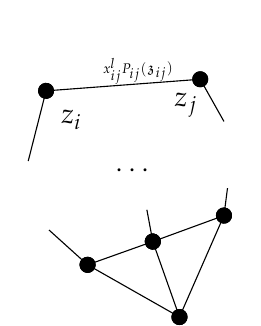
\begin{tikzpicture}[x=0.75pt,y=0.75pt,yscale=-1,xscale=1]
%uncomment if require: \path (0,214); %set diagram left start at 0, and has height of 214

%Straight Lines [id:da5823024143210767]
\draw    (318.95,172.29) -- (306.1,135.94) ;
\draw [shift={(306.1,135.94)}, rotate = 250.52] [color={rgb, 255:red, 0; green, 0; blue, 0 }  ][fill={rgb, 255:red, 0; green, 0; blue, 0 }  ][line width=0.75]      (0, 0) circle [x radius= 3.35, y radius= 3.35]   ;
\draw [shift={(318.95,172.29)}, rotate = 250.52] [color={rgb, 255:red, 0; green, 0; blue, 0 }  ][fill={rgb, 255:red, 0; green, 0; blue, 0 }  ][line width=0.75]      (0, 0) circle [x radius= 3.35, y radius= 3.35]   ;
%Straight Lines [id:da8147858505316599]
\draw    (328.95,57.74) -- (254.67,63.33) ;
\draw [shift={(254.67,63.33)}, rotate = 175.7] [color={rgb, 255:red, 0; green, 0; blue, 0 }  ][fill={rgb, 255:red, 0; green, 0; blue, 0 }  ][line width=0.75]      (0, 0) circle [x radius= 3.35, y radius= 3.35]   ;
\draw [shift={(328.95,57.74)}, rotate = 175.7] [color={rgb, 255:red, 0; green, 0; blue, 0 }  ][fill={rgb, 255:red, 0; green, 0; blue, 0 }  ][line width=0.75]      (0, 0) circle [x radius= 3.35, y radius= 3.35]   ;
%Straight Lines [id:da07628695201790259]
\draw    (274.67,147.14) -- (306.1,135.94) ;
\draw [shift={(306.1,135.94)}, rotate = 340.37] [color={rgb, 255:red, 0; green, 0; blue, 0 }  ][fill={rgb, 255:red, 0; green, 0; blue, 0 }  ][line width=0.75]      (0, 0) circle [x radius= 3.35, y radius= 3.35]   ;
\draw [shift={(274.67,147.14)}, rotate = 340.37] [color={rgb, 255:red, 0; green, 0; blue, 0 }  ][fill={rgb, 255:red, 0; green, 0; blue, 0 }  ][line width=0.75]      (0, 0) circle [x radius= 3.35, y radius= 3.35]   ;
%Straight Lines [id:da19384431212872455]
\draw    (274.67,147.14) -- (318.95,172.29) ;
\draw [shift={(318.95,172.29)}, rotate = 29.59] [color={rgb, 255:red, 0; green, 0; blue, 0 }  ][fill={rgb, 255:red, 0; green, 0; blue, 0 }  ][line width=0.75]      (0, 0) circle [x radius= 3.35, y radius= 3.35]   ;
\draw [shift={(274.67,147.14)}, rotate = 29.59] [color={rgb, 255:red, 0; green, 0; blue, 0 }  ][fill={rgb, 255:red, 0; green, 0; blue, 0 }  ][line width=0.75]      (0, 0) circle [x radius= 3.35, y radius= 3.35]   ;
%Straight Lines [id:da6790651752661128]
\draw    (254.67,63.33) -- (246.08,97.12) ;
\draw [shift={(254.67,63.33)}, rotate = 104.26] [color={rgb, 255:red, 0; green, 0; blue, 0 }  ][fill={rgb, 255:red, 0; green, 0; blue, 0 }  ][line width=0.75]      (0, 0) circle [x radius= 3.35, y radius= 3.35]   ;
%Straight Lines [id:da9419467958720287]
\draw    (328.95,57.74) -- (340.38,78.07) ;
\draw [shift={(328.95,57.74)}, rotate = 60.66] [color={rgb, 255:red, 0; green, 0; blue, 0 }  ][fill={rgb, 255:red, 0; green, 0; blue, 0 }  ][line width=0.75]      (0, 0) circle [x radius= 3.35, y radius= 3.35]   ;
%Straight Lines [id:da5446816494299196]
\draw    (306.1,135.94) -- (340.38,123.4) ;
\draw [shift={(340.38,123.4)}, rotate = 339.91] [color={rgb, 255:red, 0; green, 0; blue, 0 }  ][fill={rgb, 255:red, 0; green, 0; blue, 0 }  ][line width=0.75]      (0, 0) circle [x radius= 3.35, y radius= 3.35]   ;
\draw [shift={(306.1,135.94)}, rotate = 339.91] [color={rgb, 255:red, 0; green, 0; blue, 0 }  ][fill={rgb, 255:red, 0; green, 0; blue, 0 }  ][line width=0.75]      (0, 0) circle [x radius= 3.35, y radius= 3.35]   ;
%Straight Lines [id:da5595647047388295]
\draw    (274.67,147.14) -- (256.1,130.38) ;
\draw [shift={(274.67,147.14)}, rotate = 222.07] [color={rgb, 255:red, 0; green, 0; blue, 0 }  ][fill={rgb, 255:red, 0; green, 0; blue, 0 }  ][line width=0.75]      (0, 0) circle [x radius= 3.35, y radius= 3.35]   ;
%Straight Lines [id:da8588411657017472]
\draw    (306.1,135.94) -- (303.24,120.6) ;
\draw [shift={(306.1,135.94)}, rotate = 259.45] [color={rgb, 255:red, 0; green, 0; blue, 0 }  ][fill={rgb, 255:red, 0; green, 0; blue, 0 }  ][line width=0.75]      (0, 0) circle [x radius= 3.35, y radius= 3.35]   ;
%Straight Lines [id:da103614605215544]
\draw    (340.38,123.4) -- (342.08,110.21) ;
\draw [shift={(340.38,123.4)}, rotate = 277.36] [color={rgb, 255:red, 0; green, 0; blue, 0 }  ][fill={rgb, 255:red, 0; green, 0; blue, 0 }  ][line width=0.75]      (0, 0) circle [x radius= 3.35, y radius= 3.35]   ;
%Straight Lines [id:da4242958639619645]
\draw    (318.95,172.29) -- (340.38,123.4) ;
\draw [shift={(340.38,123.4)}, rotate = 293.67] [color={rgb, 255:red, 0; green, 0; blue, 0 }  ][fill={rgb, 255:red, 0; green, 0; blue, 0 }  ][line width=0.75]      (0, 0) circle [x radius= 3.35, y radius= 3.35]   ;
\draw [shift={(318.95,172.29)}, rotate = 293.67] [color={rgb, 255:red, 0; green, 0; blue, 0 }  ][fill={rgb, 255:red, 0; green, 0; blue, 0 }  ][line width=0.75]      (0, 0) circle [x radius= 3.35, y radius= 3.35]   ;

% Text Node
\draw (315.1,63.11) node [anchor=north west][inner sep=0.75pt]    {$z_{j}{}$};
% Text Node
\draw (260.53,71.49) node [anchor=north west][inner sep=0.75pt]    {$z_{i}$};
% Text Node
\draw (286.48,97.71) node [anchor=north west][inner sep=0.75pt]    {$\cdots $};
% Text Node
\draw (280.78,46.54) node [anchor=north west][inner sep=0.75pt]  [font=\tiny,rotate=-359.06]  {$x_{ij}^{l} P_{ij}(\mathfrak{z}_{ij})$};


\end{tikzpicture}
  \caption{}\label{}
\end{figure}
\begin{proof}
\Gui{Fill in the proof}
Using Lemma \ref{IntegralXP}, we have
$$
x^l_{ij}P_{ij}(\mathfrak{z}_{ij})=-\partial_{\mathfrak{z}_{ij}}\int^1_0P_{ij}(s\mathfrak{z}_{ij})ds.
$$
Then
\begin{align*}
   \mu_{\{1\dots n\}}\left(W_{\Gamma}(\mathfrak{z}_{e})\cdot x^l_{ij}\right)  &=\mu_{\{1\dots n\}}\left(-\partial_{\mathfrak{z}_{ij}}\int^1_0W_{\Gamma}(\dots,s\mathfrak{z}_{ij},\dots)ds\right)  \\
   & =-\partial_{\mathfrak{z}_{ij}}\int^1_0\mu_{\{1\dots n\}}\left(W_{\Gamma}(\dots,s\mathfrak{z}_{ij},\dots)\right)ds\\
   &=-\partial_{\mathfrak{z}^l_{ij}}\int^1_0F(\lambda_1,\dots,\lambda_{n-1};\dots,s\mathfrak{z}_{ij},\dots)ds.
\end{align*}
\end{proof}


\begin{lem}\label{IntegralS}
  Suppose that we have a graph with vertices $\{1,\dots,n\}$ and $i,j\subset \{1,\dots,n\}$ such that $(i,j)\in E_{\Gamma}$. Then
  $$
  \mu_{\{\star\bullet\}}\circ \mu_{\{1\dots n\}}\left(\alpha\cdot x^l_{\star i}P_{\star j }\right)=\int^1_0 F_{\alpha}(\lambda_1,\dots,\lambda_i+(1-s_{\star})\lambda_{\star},\dots,\lambda_j+s_{\star}\lambda_{\star},\lambda_{n-1};\mathfrak{z}_e)\cdot s_{\star}\lambda^l_{\star}ds_{\star}
  $$
    $$
  \mu_{\{\star\bullet\}}\circ \mu_{\{1\dots n\}}\left(\alpha\cdot x^l_{\star j}P_{\star i }\right)=\int^1_0 F_{\alpha}(\lambda_1,\dots,\lambda_i+(1-s_{\star})\lambda_{\star},\dots,\lambda_j+s_{\star}\lambda_{\star},\lambda_{n-1};\mathfrak{z}_e)\cdot(1-s_{\star})\lambda^l_{\star}ds_{\star}
  $$
  Similarly, if $\star$ is joint with $(o,i)\in E_{\Gamma}$, then
  $$
  \mu_{\{\star\bullet\}}\circ \mu_{\{1\dots n\}}\left(\alpha\cdot x^l_{\star i}P_{\star o }\right)=\int^1_0 F_{\alpha}(\lambda_1,\dots,\lambda_i+(1-s_{\star})\lambda_{\star},\dots,\lambda_{n};\mathfrak{z}_e)\cdot s_{\star}\lambda^l_{\star}ds_{\star}
  $$
   $$
  \mu_{\{\star\bullet\}}\circ \mu_{\{1\dots n\}}\left(\alpha\cdot x^l_{\star o}P_{\star i}\right)=\int^1_0 F_{\alpha}(\lambda_1,\dots,\lambda_i+(1-s_{\star})\lambda_{\star},\dots,\lambda_{n};\mathfrak{z}_e)\cdot(1-s_{\star})\lambda^l_{\star}ds_{\star}
  $$
\end{lem}
\begin{proof}
  Write
  $$
   \mu_{\{1\dots n\}}\left(\alpha\right)=F_{\alpha}(\lambda)=\sum G(\lambda_i)H(\lambda_j).
  $$
  Then
  \begin{align*}
   &  \mu_{\{\star\bullet\}}\circ \mu_{\{1\dots n\}}\left(\alpha\cdot x^l_{\star i}P_{\star j }\right)=  \mu_{\{\star\bullet\}}\left(\sum G(\lambda_i-\partial_{z_{\star}})x^l_{\star\bullet}\cdot H(\lambda_j-\partial_{z_{\star}})P_{\star\bullet}\right)\\
     &=\mu_{\{\star\bullet\}}\left(\int^1_0\sum G(\lambda_i-(1-s)\partial_{z_{\star}}) H(\lambda_j-s\partial_{z_{\star}})(-s\partial_{z^l_{\star}})P_{\star\bullet}ds\right)\quad \text{using Lemma \ref{IntegralXP}}\\
     &=\int^1_0\sum G(\lambda_i+(1-s)\lambda_{\star}) H(\lambda_j+s\lambda_{\star})(s\lambda^l_{\star})ds\\
     &=\int^1_0 F_{\alpha}(\lambda_1,\dots,\lambda_i+(1-s_{\star})\lambda_{\star},\dots,\lambda_j+s_{\star}\lambda_{\star},\lambda_{n-1};\mathfrak{z}_e)\cdot(s_{\star}\lambda^l_{\star})ds_{\star}.
  \end{align*}
\end{proof}
\begin{figure}[htp]
  \centering


\tikzset{every picture/.style={line width=0.75pt}} %set default line width to 0.75pt

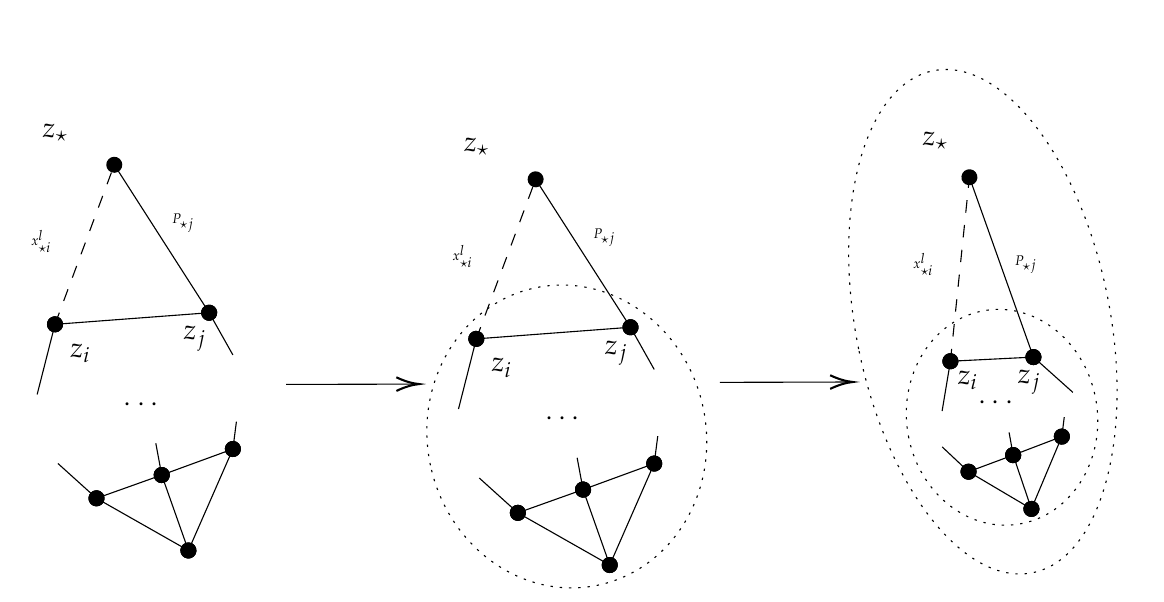
\begin{tikzpicture}[x=0.75pt,y=0.75pt,yscale=-1,xscale=1]
%uncomment if require: \path (0,300); %set diagram left start at 0, and has height of 300

%Straight Lines [id:da8577423121720247]
\draw  [dash pattern={on 4.5pt off 4.5pt}]  (60.67,131.04) -- (89.24,54.17) ;
\draw [shift={(89.24,54.17)}, rotate = 290.39] [color={rgb, 255:red, 0; green, 0; blue, 0 }  ][fill={rgb, 255:red, 0; green, 0; blue, 0 }  ][line width=0.75]      (0, 0) circle [x radius= 3.35, y radius= 3.35]   ;
\draw [shift={(60.67,131.04)}, rotate = 290.39] [color={rgb, 255:red, 0; green, 0; blue, 0 }  ][fill={rgb, 255:red, 0; green, 0; blue, 0 }  ][line width=0.75]      (0, 0) circle [x radius= 3.35, y radius= 3.35]   ;
%Straight Lines [id:da13261678783310793]
\draw    (134.95,125.45) -- (89.24,54.17) ;
\draw [shift={(134.95,125.45)}, rotate = 237.33] [color={rgb, 255:red, 0; green, 0; blue, 0 }  ][fill={rgb, 255:red, 0; green, 0; blue, 0 }  ][line width=0.75]      (0, 0) circle [x radius= 3.35, y radius= 3.35]   ;
%Straight Lines [id:da9919861590399197]
\draw    (124.95,240) -- (112.1,203.65) ;
\draw [shift={(112.1,203.65)}, rotate = 250.52] [color={rgb, 255:red, 0; green, 0; blue, 0 }  ][fill={rgb, 255:red, 0; green, 0; blue, 0 }  ][line width=0.75]      (0, 0) circle [x radius= 3.35, y radius= 3.35]   ;
\draw [shift={(124.95,240)}, rotate = 250.52] [color={rgb, 255:red, 0; green, 0; blue, 0 }  ][fill={rgb, 255:red, 0; green, 0; blue, 0 }  ][line width=0.75]      (0, 0) circle [x radius= 3.35, y radius= 3.35]   ;
%Straight Lines [id:da9722937517393717]
\draw    (134.95,125.45) -- (60.67,131.04) ;
\draw [shift={(60.67,131.04)}, rotate = 175.7] [color={rgb, 255:red, 0; green, 0; blue, 0 }  ][fill={rgb, 255:red, 0; green, 0; blue, 0 }  ][line width=0.75]      (0, 0) circle [x radius= 3.35, y radius= 3.35]   ;
\draw [shift={(134.95,125.45)}, rotate = 175.7] [color={rgb, 255:red, 0; green, 0; blue, 0 }  ][fill={rgb, 255:red, 0; green, 0; blue, 0 }  ][line width=0.75]      (0, 0) circle [x radius= 3.35, y radius= 3.35]   ;
%Straight Lines [id:da5603964973358293]
\draw    (80.67,214.86) -- (112.1,203.65) ;
\draw [shift={(112.1,203.65)}, rotate = 340.37] [color={rgb, 255:red, 0; green, 0; blue, 0 }  ][fill={rgb, 255:red, 0; green, 0; blue, 0 }  ][line width=0.75]      (0, 0) circle [x radius= 3.35, y radius= 3.35]   ;
\draw [shift={(80.67,214.86)}, rotate = 340.37] [color={rgb, 255:red, 0; green, 0; blue, 0 }  ][fill={rgb, 255:red, 0; green, 0; blue, 0 }  ][line width=0.75]      (0, 0) circle [x radius= 3.35, y radius= 3.35]   ;
%Straight Lines [id:da7092464873841009]
\draw    (80.67,214.86) -- (124.95,240) ;
\draw [shift={(124.95,240)}, rotate = 29.59] [color={rgb, 255:red, 0; green, 0; blue, 0 }  ][fill={rgb, 255:red, 0; green, 0; blue, 0 }  ][line width=0.75]      (0, 0) circle [x radius= 3.35, y radius= 3.35]   ;
\draw [shift={(80.67,214.86)}, rotate = 29.59] [color={rgb, 255:red, 0; green, 0; blue, 0 }  ][fill={rgb, 255:red, 0; green, 0; blue, 0 }  ][line width=0.75]      (0, 0) circle [x radius= 3.35, y radius= 3.35]   ;
%Straight Lines [id:da6671996787964425]
\draw    (60.67,131.04) -- (52.08,164.83) ;
\draw [shift={(60.67,131.04)}, rotate = 104.26] [color={rgb, 255:red, 0; green, 0; blue, 0 }  ][fill={rgb, 255:red, 0; green, 0; blue, 0 }  ][line width=0.75]      (0, 0) circle [x radius= 3.35, y radius= 3.35]   ;
%Straight Lines [id:da8921967722630684]
\draw    (134.95,125.45) -- (146.38,145.78) ;
\draw [shift={(134.95,125.45)}, rotate = 60.66] [color={rgb, 255:red, 0; green, 0; blue, 0 }  ][fill={rgb, 255:red, 0; green, 0; blue, 0 }  ][line width=0.75]      (0, 0) circle [x radius= 3.35, y radius= 3.35]   ;
%Straight Lines [id:da8599628892483835]
\draw    (112.1,203.65) -- (146.38,191.11) ;
\draw [shift={(146.38,191.11)}, rotate = 339.91] [color={rgb, 255:red, 0; green, 0; blue, 0 }  ][fill={rgb, 255:red, 0; green, 0; blue, 0 }  ][line width=0.75]      (0, 0) circle [x radius= 3.35, y radius= 3.35]   ;
\draw [shift={(112.1,203.65)}, rotate = 339.91] [color={rgb, 255:red, 0; green, 0; blue, 0 }  ][fill={rgb, 255:red, 0; green, 0; blue, 0 }  ][line width=0.75]      (0, 0) circle [x radius= 3.35, y radius= 3.35]   ;
%Straight Lines [id:da601234034482129]
\draw    (80.67,214.86) -- (62.1,198.09) ;
\draw [shift={(80.67,214.86)}, rotate = 222.07] [color={rgb, 255:red, 0; green, 0; blue, 0 }  ][fill={rgb, 255:red, 0; green, 0; blue, 0 }  ][line width=0.75]      (0, 0) circle [x radius= 3.35, y radius= 3.35]   ;
%Straight Lines [id:da7733669878066225]
\draw    (112.1,203.65) -- (109.24,188.31) ;
\draw [shift={(112.1,203.65)}, rotate = 259.45] [color={rgb, 255:red, 0; green, 0; blue, 0 }  ][fill={rgb, 255:red, 0; green, 0; blue, 0 }  ][line width=0.75]      (0, 0) circle [x radius= 3.35, y radius= 3.35]   ;
%Straight Lines [id:da22739188659656895]
\draw    (146.38,191.11) -- (148.08,177.92) ;
\draw [shift={(146.38,191.11)}, rotate = 277.36] [color={rgb, 255:red, 0; green, 0; blue, 0 }  ][fill={rgb, 255:red, 0; green, 0; blue, 0 }  ][line width=0.75]      (0, 0) circle [x radius= 3.35, y radius= 3.35]   ;
%Straight Lines [id:da28359362079359074]
\draw    (124.95,240) -- (146.38,191.11) ;
\draw [shift={(146.38,191.11)}, rotate = 293.67] [color={rgb, 255:red, 0; green, 0; blue, 0 }  ][fill={rgb, 255:red, 0; green, 0; blue, 0 }  ][line width=0.75]      (0, 0) circle [x radius= 3.35, y radius= 3.35]   ;
\draw [shift={(124.95,240)}, rotate = 293.67] [color={rgb, 255:red, 0; green, 0; blue, 0 }  ][fill={rgb, 255:red, 0; green, 0; blue, 0 }  ][line width=0.75]      (0, 0) circle [x radius= 3.35, y radius= 3.35]   ;
%Straight Lines [id:da44851088359116265]
\draw    (172,160) -- (234.08,159.83) ;
\draw [shift={(236.08,159.82)}, rotate = 179.84] [color={rgb, 255:red, 0; green, 0; blue, 0 }  ][line width=0.75]    (10.93,-3.29) .. controls (6.95,-1.4) and (3.31,-0.3) .. (0,0) .. controls (3.31,0.3) and (6.95,1.4) .. (10.93,3.29)   ;
%Straight Lines [id:da38480407885565926]
\draw  [dash pattern={on 4.5pt off 4.5pt}]  (263.67,138.04) -- (292.24,61.17) ;
\draw [shift={(292.24,61.17)}, rotate = 290.39] [color={rgb, 255:red, 0; green, 0; blue, 0 }  ][fill={rgb, 255:red, 0; green, 0; blue, 0 }  ][line width=0.75]      (0, 0) circle [x radius= 3.35, y radius= 3.35]   ;
\draw [shift={(263.67,138.04)}, rotate = 290.39] [color={rgb, 255:red, 0; green, 0; blue, 0 }  ][fill={rgb, 255:red, 0; green, 0; blue, 0 }  ][line width=0.75]      (0, 0) circle [x radius= 3.35, y radius= 3.35]   ;
%Straight Lines [id:da5307717551850348]
\draw    (337.95,132.45) -- (292.24,61.17) ;
\draw [shift={(337.95,132.45)}, rotate = 237.33] [color={rgb, 255:red, 0; green, 0; blue, 0 }  ][fill={rgb, 255:red, 0; green, 0; blue, 0 }  ][line width=0.75]      (0, 0) circle [x radius= 3.35, y radius= 3.35]   ;
%Straight Lines [id:da9413038592812624]
\draw    (327.95,247) -- (315.1,210.65) ;
\draw [shift={(315.1,210.65)}, rotate = 250.52] [color={rgb, 255:red, 0; green, 0; blue, 0 }  ][fill={rgb, 255:red, 0; green, 0; blue, 0 }  ][line width=0.75]      (0, 0) circle [x radius= 3.35, y radius= 3.35]   ;
\draw [shift={(327.95,247)}, rotate = 250.52] [color={rgb, 255:red, 0; green, 0; blue, 0 }  ][fill={rgb, 255:red, 0; green, 0; blue, 0 }  ][line width=0.75]      (0, 0) circle [x radius= 3.35, y radius= 3.35]   ;
%Straight Lines [id:da5150963015703387]
\draw    (337.95,132.45) -- (263.67,138.04) ;
\draw [shift={(263.67,138.04)}, rotate = 175.7] [color={rgb, 255:red, 0; green, 0; blue, 0 }  ][fill={rgb, 255:red, 0; green, 0; blue, 0 }  ][line width=0.75]      (0, 0) circle [x radius= 3.35, y radius= 3.35]   ;
\draw [shift={(337.95,132.45)}, rotate = 175.7] [color={rgb, 255:red, 0; green, 0; blue, 0 }  ][fill={rgb, 255:red, 0; green, 0; blue, 0 }  ][line width=0.75]      (0, 0) circle [x radius= 3.35, y radius= 3.35]   ;
%Straight Lines [id:da16397146641636162]
\draw    (283.67,221.86) -- (315.1,210.65) ;
\draw [shift={(315.1,210.65)}, rotate = 340.37] [color={rgb, 255:red, 0; green, 0; blue, 0 }  ][fill={rgb, 255:red, 0; green, 0; blue, 0 }  ][line width=0.75]      (0, 0) circle [x radius= 3.35, y radius= 3.35]   ;
\draw [shift={(283.67,221.86)}, rotate = 340.37] [color={rgb, 255:red, 0; green, 0; blue, 0 }  ][fill={rgb, 255:red, 0; green, 0; blue, 0 }  ][line width=0.75]      (0, 0) circle [x radius= 3.35, y radius= 3.35]   ;
%Straight Lines [id:da8143076274162886]
\draw    (283.67,221.86) -- (327.95,247) ;
\draw [shift={(327.95,247)}, rotate = 29.59] [color={rgb, 255:red, 0; green, 0; blue, 0 }  ][fill={rgb, 255:red, 0; green, 0; blue, 0 }  ][line width=0.75]      (0, 0) circle [x radius= 3.35, y radius= 3.35]   ;
\draw [shift={(283.67,221.86)}, rotate = 29.59] [color={rgb, 255:red, 0; green, 0; blue, 0 }  ][fill={rgb, 255:red, 0; green, 0; blue, 0 }  ][line width=0.75]      (0, 0) circle [x radius= 3.35, y radius= 3.35]   ;
%Straight Lines [id:da5832319766099261]
\draw    (263.67,138.04) -- (255.08,171.83) ;
\draw [shift={(263.67,138.04)}, rotate = 104.26] [color={rgb, 255:red, 0; green, 0; blue, 0 }  ][fill={rgb, 255:red, 0; green, 0; blue, 0 }  ][line width=0.75]      (0, 0) circle [x radius= 3.35, y radius= 3.35]   ;
%Straight Lines [id:da9359335501825665]
\draw    (337.95,132.45) -- (349.38,152.78) ;
\draw [shift={(337.95,132.45)}, rotate = 60.66] [color={rgb, 255:red, 0; green, 0; blue, 0 }  ][fill={rgb, 255:red, 0; green, 0; blue, 0 }  ][line width=0.75]      (0, 0) circle [x radius= 3.35, y radius= 3.35]   ;
%Straight Lines [id:da1782726456669681]
\draw    (315.1,210.65) -- (349.38,198.11) ;
\draw [shift={(349.38,198.11)}, rotate = 339.91] [color={rgb, 255:red, 0; green, 0; blue, 0 }  ][fill={rgb, 255:red, 0; green, 0; blue, 0 }  ][line width=0.75]      (0, 0) circle [x radius= 3.35, y radius= 3.35]   ;
\draw [shift={(315.1,210.65)}, rotate = 339.91] [color={rgb, 255:red, 0; green, 0; blue, 0 }  ][fill={rgb, 255:red, 0; green, 0; blue, 0 }  ][line width=0.75]      (0, 0) circle [x radius= 3.35, y radius= 3.35]   ;
%Straight Lines [id:da7217720127600564]
\draw    (283.67,221.86) -- (265.1,205.09) ;
\draw [shift={(283.67,221.86)}, rotate = 222.07] [color={rgb, 255:red, 0; green, 0; blue, 0 }  ][fill={rgb, 255:red, 0; green, 0; blue, 0 }  ][line width=0.75]      (0, 0) circle [x radius= 3.35, y radius= 3.35]   ;
%Straight Lines [id:da9726191077362507]
\draw    (315.1,210.65) -- (312.24,195.31) ;
\draw [shift={(315.1,210.65)}, rotate = 259.45] [color={rgb, 255:red, 0; green, 0; blue, 0 }  ][fill={rgb, 255:red, 0; green, 0; blue, 0 }  ][line width=0.75]      (0, 0) circle [x radius= 3.35, y radius= 3.35]   ;
%Straight Lines [id:da9228840677417147]
\draw    (349.38,198.11) -- (351.08,184.92) ;
\draw [shift={(349.38,198.11)}, rotate = 277.36] [color={rgb, 255:red, 0; green, 0; blue, 0 }  ][fill={rgb, 255:red, 0; green, 0; blue, 0 }  ][line width=0.75]      (0, 0) circle [x radius= 3.35, y radius= 3.35]   ;
%Straight Lines [id:da7187239691883223]
\draw    (327.95,247) -- (349.38,198.11) ;
\draw [shift={(349.38,198.11)}, rotate = 293.67] [color={rgb, 255:red, 0; green, 0; blue, 0 }  ][fill={rgb, 255:red, 0; green, 0; blue, 0 }  ][line width=0.75]      (0, 0) circle [x radius= 3.35, y radius= 3.35]   ;
\draw [shift={(327.95,247)}, rotate = 293.67] [color={rgb, 255:red, 0; green, 0; blue, 0 }  ][fill={rgb, 255:red, 0; green, 0; blue, 0 }  ][line width=0.75]      (0, 0) circle [x radius= 3.35, y radius= 3.35]   ;
%Shape: Ellipse [id:dp4777570083321534]
\draw  [dash pattern={on 0.84pt off 2.51pt}] (241.56,198.94) .. controls (233.21,159.38) and (255.86,121.1) .. (292.14,113.44) .. controls (328.43,105.78) and (364.61,131.64) .. (372.96,171.2) .. controls (381.31,210.76) and (358.67,249.03) .. (322.38,256.69) .. controls (286.1,264.35) and (249.91,238.49) .. (241.56,198.94) -- cycle ;
%Straight Lines [id:da2717921113507169]
\draw    (381,159) -- (443.08,158.83) ;
\draw [shift={(445.08,158.82)}, rotate = 179.84] [color={rgb, 255:red, 0; green, 0; blue, 0 }  ][line width=0.75]    (10.93,-3.29) .. controls (6.95,-1.4) and (3.31,-0.3) .. (0,0) .. controls (3.31,0.3) and (6.95,1.4) .. (10.93,3.29)   ;
%Straight Lines [id:da9369417437849918]
\draw  [dash pattern={on 4.5pt off 4.5pt}]  (492.08,148.82) -- (501.24,60.17) ;
\draw [shift={(501.24,60.17)}, rotate = 275.9] [color={rgb, 255:red, 0; green, 0; blue, 0 }  ][fill={rgb, 255:red, 0; green, 0; blue, 0 }  ][line width=0.75]      (0, 0) circle [x radius= 3.35, y radius= 3.35]   ;
\draw [shift={(492.08,148.82)}, rotate = 275.9] [color={rgb, 255:red, 0; green, 0; blue, 0 }  ][fill={rgb, 255:red, 0; green, 0; blue, 0 }  ][line width=0.75]      (0, 0) circle [x radius= 3.35, y radius= 3.35]   ;
%Straight Lines [id:da9853072568986168]
\draw    (532.08,146.82) -- (501.24,60.17) ;
\draw [shift={(532.08,146.82)}, rotate = 250.41] [color={rgb, 255:red, 0; green, 0; blue, 0 }  ][fill={rgb, 255:red, 0; green, 0; blue, 0 }  ][line width=0.75]      (0, 0) circle [x radius= 3.35, y radius= 3.35]   ;
%Straight Lines [id:da41602927139069523]
\draw    (531.11,219.96) -- (522.32,194.05) ;
\draw [shift={(522.32,194.05)}, rotate = 251.25] [color={rgb, 255:red, 0; green, 0; blue, 0 }  ][fill={rgb, 255:red, 0; green, 0; blue, 0 }  ][line width=0.75]      (0, 0) circle [x radius= 3.35, y radius= 3.35]   ;
\draw [shift={(531.11,219.96)}, rotate = 251.25] [color={rgb, 255:red, 0; green, 0; blue, 0 }  ][fill={rgb, 255:red, 0; green, 0; blue, 0 }  ][line width=0.75]      (0, 0) circle [x radius= 3.35, y radius= 3.35]   ;
%Straight Lines [id:da4586830007929794]
\draw    (532.08,146.82) -- (492.08,148.82) ;
\draw [shift={(492.08,148.82)}, rotate = 177.14] [color={rgb, 255:red, 0; green, 0; blue, 0 }  ][fill={rgb, 255:red, 0; green, 0; blue, 0 }  ][line width=0.75]      (0, 0) circle [x radius= 3.35, y radius= 3.35]   ;
\draw [shift={(532.08,146.82)}, rotate = 177.14] [color={rgb, 255:red, 0; green, 0; blue, 0 }  ][fill={rgb, 255:red, 0; green, 0; blue, 0 }  ][line width=0.75]      (0, 0) circle [x radius= 3.35, y radius= 3.35]   ;
%Straight Lines [id:da8800919049561395]
\draw    (500.82,202.04) -- (522.32,194.05) ;
\draw [shift={(522.32,194.05)}, rotate = 339.62] [color={rgb, 255:red, 0; green, 0; blue, 0 }  ][fill={rgb, 255:red, 0; green, 0; blue, 0 }  ][line width=0.75]      (0, 0) circle [x radius= 3.35, y radius= 3.35]   ;
\draw [shift={(500.82,202.04)}, rotate = 339.62] [color={rgb, 255:red, 0; green, 0; blue, 0 }  ][fill={rgb, 255:red, 0; green, 0; blue, 0 }  ][line width=0.75]      (0, 0) circle [x radius= 3.35, y radius= 3.35]   ;
%Straight Lines [id:da09222954685831342]
\draw    (500.82,202.04) -- (531.11,219.96) ;
\draw [shift={(531.11,219.96)}, rotate = 30.61] [color={rgb, 255:red, 0; green, 0; blue, 0 }  ][fill={rgb, 255:red, 0; green, 0; blue, 0 }  ][line width=0.75]      (0, 0) circle [x radius= 3.35, y radius= 3.35]   ;
\draw [shift={(500.82,202.04)}, rotate = 30.61] [color={rgb, 255:red, 0; green, 0; blue, 0 }  ][fill={rgb, 255:red, 0; green, 0; blue, 0 }  ][line width=0.75]      (0, 0) circle [x radius= 3.35, y radius= 3.35]   ;
%Straight Lines [id:da4563450226607171]
\draw    (492.08,148.82) -- (488.08,172.82) ;
\draw [shift={(492.08,148.82)}, rotate = 99.46] [color={rgb, 255:red, 0; green, 0; blue, 0 }  ][fill={rgb, 255:red, 0; green, 0; blue, 0 }  ][line width=0.75]      (0, 0) circle [x radius= 3.35, y radius= 3.35]   ;
%Straight Lines [id:da20087686932634408]
\draw    (532.08,146.82) -- (551.08,163.82) ;
\draw [shift={(532.08,146.82)}, rotate = 41.82] [color={rgb, 255:red, 0; green, 0; blue, 0 }  ][fill={rgb, 255:red, 0; green, 0; blue, 0 }  ][line width=0.75]      (0, 0) circle [x radius= 3.35, y radius= 3.35]   ;
%Straight Lines [id:da9710477288628783]
\draw    (522.32,194.05) -- (545.77,185.11) ;
\draw [shift={(545.77,185.11)}, rotate = 339.14] [color={rgb, 255:red, 0; green, 0; blue, 0 }  ][fill={rgb, 255:red, 0; green, 0; blue, 0 }  ][line width=0.75]      (0, 0) circle [x radius= 3.35, y radius= 3.35]   ;
\draw [shift={(522.32,194.05)}, rotate = 339.14] [color={rgb, 255:red, 0; green, 0; blue, 0 }  ][fill={rgb, 255:red, 0; green, 0; blue, 0 }  ][line width=0.75]      (0, 0) circle [x radius= 3.35, y radius= 3.35]   ;
%Straight Lines [id:da22424434990223552]
\draw    (500.82,202.04) -- (488.12,190.09) ;
\draw [shift={(500.82,202.04)}, rotate = 223.24] [color={rgb, 255:red, 0; green, 0; blue, 0 }  ][fill={rgb, 255:red, 0; green, 0; blue, 0 }  ][line width=0.75]      (0, 0) circle [x radius= 3.35, y radius= 3.35]   ;
%Straight Lines [id:da9762485288475353]
\draw    (522.32,194.05) -- (520.36,183.12) ;
\draw [shift={(522.32,194.05)}, rotate = 259.86] [color={rgb, 255:red, 0; green, 0; blue, 0 }  ][fill={rgb, 255:red, 0; green, 0; blue, 0 }  ][line width=0.75]      (0, 0) circle [x radius= 3.35, y radius= 3.35]   ;
%Straight Lines [id:da3615614902452422]
\draw    (545.77,185.11) -- (546.93,175.72) ;
\draw [shift={(545.77,185.11)}, rotate = 277.07] [color={rgb, 255:red, 0; green, 0; blue, 0 }  ][fill={rgb, 255:red, 0; green, 0; blue, 0 }  ][line width=0.75]      (0, 0) circle [x radius= 3.35, y radius= 3.35]   ;
%Straight Lines [id:da13050800750452307]
\draw    (531.11,219.96) -- (545.77,185.11) ;
\draw [shift={(545.77,185.11)}, rotate = 292.81] [color={rgb, 255:red, 0; green, 0; blue, 0 }  ][fill={rgb, 255:red, 0; green, 0; blue, 0 }  ][line width=0.75]      (0, 0) circle [x radius= 3.35, y radius= 3.35]   ;
\draw [shift={(531.11,219.96)}, rotate = 292.81] [color={rgb, 255:red, 0; green, 0; blue, 0 }  ][fill={rgb, 255:red, 0; green, 0; blue, 0 }  ][line width=0.75]      (0, 0) circle [x radius= 3.35, y radius= 3.35]   ;
%Shape: Ellipse [id:dp8788676993480489]
\draw  [dash pattern={on 0.84pt off 2.51pt}] (472.01,185.7) .. controls (466.3,157.52) and (481.8,130.24) .. (506.62,124.78) .. controls (531.44,119.33) and (556.19,137.75) .. (561.9,165.94) .. controls (567.61,194.13) and (552.12,221.41) .. (527.3,226.86) .. controls (502.47,232.32) and (477.72,213.89) .. (472.01,185.7) -- cycle ;
%Shape: Ellipse [id:dp25977476782180076]
\draw  [dash pattern={on 0.84pt off 2.51pt}] (447.88,142.94) .. controls (434.37,76.22) and (450.2,16.24) .. (483.25,8.98) .. controls (516.3,1.71) and (554.04,49.91) .. (567.55,116.63) .. controls (581.07,183.35) and (565.23,243.32) .. (532.19,250.59) .. controls (499.14,257.85) and (461.4,209.66) .. (447.88,142.94) -- cycle ;

% Text Node
\draw (53.19,33.11) node [anchor=north west][inner sep=0.75pt]    {$z_{\star }$};
% Text Node
\draw (121.1,130.82) node [anchor=north west][inner sep=0.75pt]    {$z_{j}{}$};
% Text Node
\draw (66.53,139.2) node [anchor=north west][inner sep=0.75pt]    {$z_{i}$};
% Text Node
\draw (92.48,165.42) node [anchor=north west][inner sep=0.75pt]    {$\cdots $};
% Text Node
\draw (47.78,84.62) node [anchor=north west][inner sep=0.75pt]  [font=\tiny,rotate=-359.06]  {$x_{\star i}^{l}$};
% Text Node
\draw (115.78,76.62) node [anchor=north west][inner sep=0.75pt]  [font=\tiny,rotate=-359.06]  {$P_{\star j}$};
% Text Node
\draw (256.19,40.11) node [anchor=north west][inner sep=0.75pt]    {$z_{\star }$};
% Text Node
\draw (324.1,137.82) node [anchor=north west][inner sep=0.75pt]    {$z_{j}{}$};
% Text Node
\draw (269.53,146.2) node [anchor=north west][inner sep=0.75pt]    {$z_{i}$};
% Text Node
\draw (295.48,172.42) node [anchor=north west][inner sep=0.75pt]    {$\cdots $};
% Text Node
\draw (250.78,91.62) node [anchor=north west][inner sep=0.75pt]  [font=\tiny,rotate=-359.06]  {$x_{\star i}^{l}$};
% Text Node
\draw (318.78,83.62) node [anchor=north west][inner sep=0.75pt]  [font=\tiny,rotate=-359.06]  {$P_{\star j}$};
% Text Node
\draw (477.19,37.11) node [anchor=north west][inner sep=0.75pt]    {$z_{\star }$};
% Text Node
\draw (523.1,151.82) node [anchor=north west][inner sep=0.75pt]    {$z_{j}{}$};
% Text Node
\draw (494.08,152.22) node [anchor=north west][inner sep=0.75pt]    {$z_{i}$};
% Text Node
\draw (504.31,164.63) node [anchor=north west][inner sep=0.75pt]    {$\cdots $};
% Text Node
\draw (472.78,95.62) node [anchor=north west][inner sep=0.75pt]  [font=\tiny,rotate=-359.06]  {$x_{\star i}^{l}$};
% Text Node
\draw (521.78,96.62) node [anchor=north west][inner sep=0.75pt]  [font=\tiny,rotate=-359.06]  {$P_{\star j}$};


\end{tikzpicture}
  \caption{}\label{}
\end{figure}

\begin{figure}[htp]
  \centering


\tikzset{every picture/.style={line width=0.75pt}} %set default line width to 0.75pt

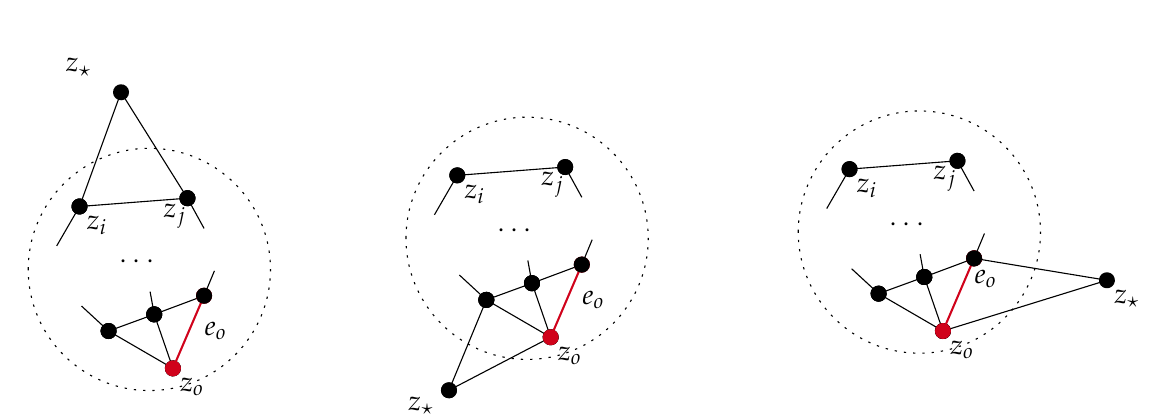
\begin{tikzpicture}[x=0.75pt,y=0.75pt,yscale=-1,xscale=1]
%uncomment if require: \path (0,283); %set diagram left start at 0, and has height of 283

%Shape: Circle [id:dp8083702044501739]
\draw  [dash pattern={on 0.84pt off 2.51pt}] (45.37,133.27) .. controls (45.37,101.05) and (71.5,74.92) .. (103.73,74.92) .. controls (135.95,74.92) and (162.08,101.05) .. (162.08,133.27) .. controls (162.08,165.5) and (135.95,191.63) .. (103.73,191.63) .. controls (71.5,191.63) and (45.37,165.5) .. (45.37,133.27) -- cycle ;
%Straight Lines [id:da41116817354603885]
\draw    (70.08,102.95) -- (90.08,47.92) ;
\draw [shift={(90.08,47.92)}, rotate = 289.98] [color={rgb, 255:red, 0; green, 0; blue, 0 }  ][fill={rgb, 255:red, 0; green, 0; blue, 0 }  ][line width=0.75]      (0, 0) circle [x radius= 3.35, y radius= 3.35]   ;
\draw [shift={(70.08,102.95)}, rotate = 289.98] [color={rgb, 255:red, 0; green, 0; blue, 0 }  ][fill={rgb, 255:red, 0; green, 0; blue, 0 }  ][line width=0.75]      (0, 0) circle [x radius= 3.35, y radius= 3.35]   ;
%Straight Lines [id:da34277569523600615]
\draw    (122.08,98.95) -- (90.08,47.92) ;
\draw [shift={(122.08,98.95)}, rotate = 237.91] [color={rgb, 255:red, 0; green, 0; blue, 0 }  ][fill={rgb, 255:red, 0; green, 0; blue, 0 }  ][line width=0.75]      (0, 0) circle [x radius= 3.35, y radius= 3.35]   ;
%Straight Lines [id:da5089975102649578]
\draw    (115.08,180.95) -- (106.08,154.92) ;
\draw [shift={(106.08,154.92)}, rotate = 250.92] [color={rgb, 255:red, 0; green, 0; blue, 0 }  ][fill={rgb, 255:red, 0; green, 0; blue, 0 }  ][line width=0.75]      (0, 0) circle [x radius= 3.35, y radius= 3.35]   ;
\draw [shift={(115.08,180.95)}, rotate = 250.92] [color={rgb, 255:red, 0; green, 0; blue, 0 }  ][fill={rgb, 255:red, 0; green, 0; blue, 0 }  ][line width=0.75]      (0, 0) circle [x radius= 3.35, y radius= 3.35]   ;
%Straight Lines [id:da5223764515960876]
\draw    (122.08,98.95) -- (70.08,102.95) ;
\draw [shift={(70.08,102.95)}, rotate = 175.6] [color={rgb, 255:red, 0; green, 0; blue, 0 }  ][fill={rgb, 255:red, 0; green, 0; blue, 0 }  ][line width=0.75]      (0, 0) circle [x radius= 3.35, y radius= 3.35]   ;
\draw [shift={(122.08,98.95)}, rotate = 175.6] [color={rgb, 255:red, 0; green, 0; blue, 0 }  ][fill={rgb, 255:red, 0; green, 0; blue, 0 }  ][line width=0.75]      (0, 0) circle [x radius= 3.35, y radius= 3.35]   ;
%Straight Lines [id:da3133816919828669]
\draw    (84.08,162.95) -- (106.08,154.92) ;
\draw [shift={(106.08,154.92)}, rotate = 339.96] [color={rgb, 255:red, 0; green, 0; blue, 0 }  ][fill={rgb, 255:red, 0; green, 0; blue, 0 }  ][line width=0.75]      (0, 0) circle [x radius= 3.35, y radius= 3.35]   ;
\draw [shift={(84.08,162.95)}, rotate = 339.96] [color={rgb, 255:red, 0; green, 0; blue, 0 }  ][fill={rgb, 255:red, 0; green, 0; blue, 0 }  ][line width=0.75]      (0, 0) circle [x radius= 3.35, y radius= 3.35]   ;
%Straight Lines [id:da2989742473880517]
\draw    (84.08,162.95) -- (115.08,180.95) ;
\draw [shift={(115.08,180.95)}, rotate = 30.14] [color={rgb, 255:red, 0; green, 0; blue, 0 }  ][fill={rgb, 255:red, 0; green, 0; blue, 0 }  ][line width=0.75]      (0, 0) circle [x radius= 3.35, y radius= 3.35]   ;
\draw [shift={(84.08,162.95)}, rotate = 30.14] [color={rgb, 255:red, 0; green, 0; blue, 0 }  ][fill={rgb, 255:red, 0; green, 0; blue, 0 }  ][line width=0.75]      (0, 0) circle [x radius= 3.35, y radius= 3.35]   ;
%Straight Lines [id:da13987264129177768]
\draw    (70.08,102.95) -- (59.08,121.95) ;
\draw [shift={(70.08,102.95)}, rotate = 120.07] [color={rgb, 255:red, 0; green, 0; blue, 0 }  ][fill={rgb, 255:red, 0; green, 0; blue, 0 }  ][line width=0.75]      (0, 0) circle [x radius= 3.35, y radius= 3.35]   ;
%Straight Lines [id:da4882856746367197]
\draw    (122.08,98.95) -- (130.08,113.5) ;
\draw [shift={(122.08,98.95)}, rotate = 61.21] [color={rgb, 255:red, 0; green, 0; blue, 0 }  ][fill={rgb, 255:red, 0; green, 0; blue, 0 }  ][line width=0.75]      (0, 0) circle [x radius= 3.35, y radius= 3.35]   ;
%Straight Lines [id:da39399358681544383]
\draw    (106.08,154.92) -- (130.08,145.95) ;
\draw [shift={(130.08,145.95)}, rotate = 339.49] [color={rgb, 255:red, 0; green, 0; blue, 0 }  ][fill={rgb, 255:red, 0; green, 0; blue, 0 }  ][line width=0.75]      (0, 0) circle [x radius= 3.35, y radius= 3.35]   ;
\draw [shift={(106.08,154.92)}, rotate = 339.49] [color={rgb, 255:red, 0; green, 0; blue, 0 }  ][fill={rgb, 255:red, 0; green, 0; blue, 0 }  ][line width=0.75]      (0, 0) circle [x radius= 3.35, y radius= 3.35]   ;
%Straight Lines [id:da021943993347968815]
\draw [color={rgb, 255:red, 208; green, 2; blue, 27 }  ,draw opacity=1 ][line width=0.75]    (115.08,180.95) -- (130.08,145.95) ;
\draw [shift={(130.08,145.95)}, rotate = 293.2] [color={rgb, 255:red, 208; green, 2; blue, 27 }  ,draw opacity=1 ][fill={rgb, 255:red, 208; green, 2; blue, 27 }  ,fill opacity=1 ][line width=0.75]      (0, 0) circle [x radius= 3.35, y radius= 3.35]   ;
\draw [shift={(115.08,180.95)}, rotate = 293.2] [color={rgb, 255:red, 208; green, 2; blue, 27 }  ,draw opacity=1 ][fill={rgb, 255:red, 208; green, 2; blue, 27 }  ,fill opacity=1 ][line width=0.75]      (0, 0) circle [x radius= 3.35, y radius= 3.35]   ;
%Straight Lines [id:da29682217038769654]
\draw    (84.08,162.95) -- (71.08,150.95) ;
\draw [shift={(84.08,162.95)}, rotate = 222.71] [color={rgb, 255:red, 0; green, 0; blue, 0 }  ][fill={rgb, 255:red, 0; green, 0; blue, 0 }  ][line width=0.75]      (0, 0) circle [x radius= 3.35, y radius= 3.35]   ;
%Straight Lines [id:da5496072141611632]
\draw    (106.08,154.92) -- (104.08,143.95) ;
\draw [shift={(106.08,154.92)}, rotate = 259.67] [color={rgb, 255:red, 0; green, 0; blue, 0 }  ][fill={rgb, 255:red, 0; green, 0; blue, 0 }  ][line width=0.75]      (0, 0) circle [x radius= 3.35, y radius= 3.35]   ;
%Straight Lines [id:da5967119205460225]
\draw    (130.08,145.95) -- (135.08,133.95) ;
\draw [shift={(130.08,145.95)}, rotate = 292.62] [color={rgb, 255:red, 0; green, 0; blue, 0 }  ][fill={rgb, 255:red, 0; green, 0; blue, 0 }  ][line width=0.75]      (0, 0) circle [x radius= 3.35, y radius= 3.35]   ;
%Shape: Circle [id:dp50413822479079]
\draw  [dash pattern={on 0.84pt off 2.51pt}] (227.37,118.27) .. controls (227.37,86.05) and (253.5,59.92) .. (285.73,59.92) .. controls (317.95,59.92) and (344.08,86.05) .. (344.08,118.27) .. controls (344.08,150.5) and (317.95,176.63) .. (285.73,176.63) .. controls (253.5,176.63) and (227.37,150.5) .. (227.37,118.27) -- cycle ;
%Straight Lines [id:da1648119557380343]
\draw    (266.08,147.95) -- (248.08,191.5) ;
\draw [shift={(248.08,191.5)}, rotate = 112.45] [color={rgb, 255:red, 0; green, 0; blue, 0 }  ][fill={rgb, 255:red, 0; green, 0; blue, 0 }  ][line width=0.75]      (0, 0) circle [x radius= 3.35, y radius= 3.35]   ;
\draw [shift={(266.08,147.95)}, rotate = 112.45] [color={rgb, 255:red, 0; green, 0; blue, 0 }  ][fill={rgb, 255:red, 0; green, 0; blue, 0 }  ][line width=0.75]      (0, 0) circle [x radius= 3.35, y radius= 3.35]   ;
%Straight Lines [id:da6236095673422983]
\draw    (248.08,191.5) -- (297.08,165.95) ;
\draw [shift={(248.08,191.5)}, rotate = 332.46] [color={rgb, 255:red, 0; green, 0; blue, 0 }  ][fill={rgb, 255:red, 0; green, 0; blue, 0 }  ][line width=0.75]      (0, 0) circle [x radius= 3.35, y radius= 3.35]   ;
%Straight Lines [id:da7220199169895192]
\draw    (297.08,165.95) -- (288.08,139.92) ;
\draw [shift={(288.08,139.92)}, rotate = 250.92] [color={rgb, 255:red, 0; green, 0; blue, 0 }  ][fill={rgb, 255:red, 0; green, 0; blue, 0 }  ][line width=0.75]      (0, 0) circle [x radius= 3.35, y radius= 3.35]   ;
\draw [shift={(297.08,165.95)}, rotate = 250.92] [color={rgb, 255:red, 0; green, 0; blue, 0 }  ][fill={rgb, 255:red, 0; green, 0; blue, 0 }  ][line width=0.75]      (0, 0) circle [x radius= 3.35, y radius= 3.35]   ;
%Straight Lines [id:da7995796109380549]
\draw    (304.08,83.95) -- (252.08,87.95) ;
\draw [shift={(252.08,87.95)}, rotate = 175.6] [color={rgb, 255:red, 0; green, 0; blue, 0 }  ][fill={rgb, 255:red, 0; green, 0; blue, 0 }  ][line width=0.75]      (0, 0) circle [x radius= 3.35, y radius= 3.35]   ;
\draw [shift={(304.08,83.95)}, rotate = 175.6] [color={rgb, 255:red, 0; green, 0; blue, 0 }  ][fill={rgb, 255:red, 0; green, 0; blue, 0 }  ][line width=0.75]      (0, 0) circle [x radius= 3.35, y radius= 3.35]   ;
%Straight Lines [id:da42111529394151104]
\draw    (266.08,147.95) -- (288.08,139.92) ;
\draw [shift={(288.08,139.92)}, rotate = 339.96] [color={rgb, 255:red, 0; green, 0; blue, 0 }  ][fill={rgb, 255:red, 0; green, 0; blue, 0 }  ][line width=0.75]      (0, 0) circle [x radius= 3.35, y radius= 3.35]   ;
\draw [shift={(266.08,147.95)}, rotate = 339.96] [color={rgb, 255:red, 0; green, 0; blue, 0 }  ][fill={rgb, 255:red, 0; green, 0; blue, 0 }  ][line width=0.75]      (0, 0) circle [x radius= 3.35, y radius= 3.35]   ;
%Straight Lines [id:da7027578449791063]
\draw    (266.08,147.95) -- (297.08,165.95) ;
\draw [shift={(297.08,165.95)}, rotate = 30.14] [color={rgb, 255:red, 0; green, 0; blue, 0 }  ][fill={rgb, 255:red, 0; green, 0; blue, 0 }  ][line width=0.75]      (0, 0) circle [x radius= 3.35, y radius= 3.35]   ;
\draw [shift={(266.08,147.95)}, rotate = 30.14] [color={rgb, 255:red, 0; green, 0; blue, 0 }  ][fill={rgb, 255:red, 0; green, 0; blue, 0 }  ][line width=0.75]      (0, 0) circle [x radius= 3.35, y radius= 3.35]   ;
%Straight Lines [id:da809651028097278]
\draw    (252.08,87.95) -- (241.08,106.95) ;
\draw [shift={(252.08,87.95)}, rotate = 120.07] [color={rgb, 255:red, 0; green, 0; blue, 0 }  ][fill={rgb, 255:red, 0; green, 0; blue, 0 }  ][line width=0.75]      (0, 0) circle [x radius= 3.35, y radius= 3.35]   ;
%Straight Lines [id:da44375980516038616]
\draw    (304.08,83.95) -- (312.08,98.5) ;
\draw [shift={(304.08,83.95)}, rotate = 61.21] [color={rgb, 255:red, 0; green, 0; blue, 0 }  ][fill={rgb, 255:red, 0; green, 0; blue, 0 }  ][line width=0.75]      (0, 0) circle [x radius= 3.35, y radius= 3.35]   ;
%Straight Lines [id:da1578506933143189]
\draw    (288.08,139.92) -- (312.08,130.95) ;
\draw [shift={(312.08,130.95)}, rotate = 339.49] [color={rgb, 255:red, 0; green, 0; blue, 0 }  ][fill={rgb, 255:red, 0; green, 0; blue, 0 }  ][line width=0.75]      (0, 0) circle [x radius= 3.35, y radius= 3.35]   ;
\draw [shift={(288.08,139.92)}, rotate = 339.49] [color={rgb, 255:red, 0; green, 0; blue, 0 }  ][fill={rgb, 255:red, 0; green, 0; blue, 0 }  ][line width=0.75]      (0, 0) circle [x radius= 3.35, y radius= 3.35]   ;
%Straight Lines [id:da2978924613859981]
\draw [color={rgb, 255:red, 208; green, 2; blue, 27 }  ,draw opacity=1 ][line width=0.75]    (297.08,165.95) -- (312.08,130.95) ;
\draw [shift={(312.08,130.95)}, rotate = 293.2] [color={rgb, 255:red, 208; green, 2; blue, 27 }  ,draw opacity=1 ][fill={rgb, 255:red, 208; green, 2; blue, 27 }  ,fill opacity=1 ][line width=0.75]      (0, 0) circle [x radius= 3.35, y radius= 3.35]   ;
\draw [shift={(297.08,165.95)}, rotate = 293.2] [color={rgb, 255:red, 208; green, 2; blue, 27 }  ,draw opacity=1 ][fill={rgb, 255:red, 208; green, 2; blue, 27 }  ,fill opacity=1 ][line width=0.75]      (0, 0) circle [x radius= 3.35, y radius= 3.35]   ;
%Straight Lines [id:da751353817269335]
\draw    (266.08,147.95) -- (253.08,135.95) ;
\draw [shift={(266.08,147.95)}, rotate = 222.71] [color={rgb, 255:red, 0; green, 0; blue, 0 }  ][fill={rgb, 255:red, 0; green, 0; blue, 0 }  ][line width=0.75]      (0, 0) circle [x radius= 3.35, y radius= 3.35]   ;
%Straight Lines [id:da7004857357994263]
\draw    (288.08,139.92) -- (286.08,128.95) ;
\draw [shift={(288.08,139.92)}, rotate = 259.67] [color={rgb, 255:red, 0; green, 0; blue, 0 }  ][fill={rgb, 255:red, 0; green, 0; blue, 0 }  ][line width=0.75]      (0, 0) circle [x radius= 3.35, y radius= 3.35]   ;
%Straight Lines [id:da8899129111575641]
\draw    (312.08,130.95) -- (317.08,118.95) ;
\draw [shift={(312.08,130.95)}, rotate = 292.62] [color={rgb, 255:red, 0; green, 0; blue, 0 }  ][fill={rgb, 255:red, 0; green, 0; blue, 0 }  ][line width=0.75]      (0, 0) circle [x radius= 3.35, y radius= 3.35]   ;
%Shape: Circle [id:dp27756615495394454]
\draw  [dash pattern={on 0.84pt off 2.51pt}] (416.37,115.27) .. controls (416.37,83.05) and (442.5,56.92) .. (474.73,56.92) .. controls (506.95,56.92) and (533.08,83.05) .. (533.08,115.27) .. controls (533.08,147.5) and (506.95,173.63) .. (474.73,173.63) .. controls (442.5,173.63) and (416.37,147.5) .. (416.37,115.27) -- cycle ;
%Straight Lines [id:da5356140973885566]
\draw    (486.08,162.95) -- (565.08,138.5) ;
\draw [shift={(565.08,138.5)}, rotate = 342.81] [color={rgb, 255:red, 0; green, 0; blue, 0 }  ][fill={rgb, 255:red, 0; green, 0; blue, 0 }  ][line width=0.75]      (0, 0) circle [x radius= 3.35, y radius= 3.35]   ;
\draw [shift={(486.08,162.95)}, rotate = 342.81] [color={rgb, 255:red, 0; green, 0; blue, 0 }  ][fill={rgb, 255:red, 0; green, 0; blue, 0 }  ][line width=0.75]      (0, 0) circle [x radius= 3.35, y radius= 3.35]   ;
%Straight Lines [id:da10459897892368053]
\draw    (501.08,127.95) -- (565.08,138.5) ;
\draw [shift={(501.08,127.95)}, rotate = 9.37] [color={rgb, 255:red, 0; green, 0; blue, 0 }  ][fill={rgb, 255:red, 0; green, 0; blue, 0 }  ][line width=0.75]      (0, 0) circle [x radius= 3.35, y radius= 3.35]   ;
%Straight Lines [id:da975342800099781]
\draw    (486.08,162.95) -- (477.08,136.92) ;
\draw [shift={(477.08,136.92)}, rotate = 250.92] [color={rgb, 255:red, 0; green, 0; blue, 0 }  ][fill={rgb, 255:red, 0; green, 0; blue, 0 }  ][line width=0.75]      (0, 0) circle [x radius= 3.35, y radius= 3.35]   ;
\draw [shift={(486.08,162.95)}, rotate = 250.92] [color={rgb, 255:red, 0; green, 0; blue, 0 }  ][fill={rgb, 255:red, 0; green, 0; blue, 0 }  ][line width=0.75]      (0, 0) circle [x radius= 3.35, y radius= 3.35]   ;
%Straight Lines [id:da22197817063182357]
\draw    (493.08,80.95) -- (441.08,84.95) ;
\draw [shift={(441.08,84.95)}, rotate = 175.6] [color={rgb, 255:red, 0; green, 0; blue, 0 }  ][fill={rgb, 255:red, 0; green, 0; blue, 0 }  ][line width=0.75]      (0, 0) circle [x radius= 3.35, y radius= 3.35]   ;
\draw [shift={(493.08,80.95)}, rotate = 175.6] [color={rgb, 255:red, 0; green, 0; blue, 0 }  ][fill={rgb, 255:red, 0; green, 0; blue, 0 }  ][line width=0.75]      (0, 0) circle [x radius= 3.35, y radius= 3.35]   ;
%Straight Lines [id:da006672829780088874]
\draw    (455.08,144.95) -- (477.08,136.92) ;
\draw [shift={(477.08,136.92)}, rotate = 339.96] [color={rgb, 255:red, 0; green, 0; blue, 0 }  ][fill={rgb, 255:red, 0; green, 0; blue, 0 }  ][line width=0.75]      (0, 0) circle [x radius= 3.35, y radius= 3.35]   ;
\draw [shift={(455.08,144.95)}, rotate = 339.96] [color={rgb, 255:red, 0; green, 0; blue, 0 }  ][fill={rgb, 255:red, 0; green, 0; blue, 0 }  ][line width=0.75]      (0, 0) circle [x radius= 3.35, y radius= 3.35]   ;
%Straight Lines [id:da7126610945382026]
\draw    (455.08,144.95) -- (486.08,162.95) ;
\draw [shift={(486.08,162.95)}, rotate = 30.14] [color={rgb, 255:red, 0; green, 0; blue, 0 }  ][fill={rgb, 255:red, 0; green, 0; blue, 0 }  ][line width=0.75]      (0, 0) circle [x radius= 3.35, y radius= 3.35]   ;
\draw [shift={(455.08,144.95)}, rotate = 30.14] [color={rgb, 255:red, 0; green, 0; blue, 0 }  ][fill={rgb, 255:red, 0; green, 0; blue, 0 }  ][line width=0.75]      (0, 0) circle [x radius= 3.35, y radius= 3.35]   ;
%Straight Lines [id:da6914016042034301]
\draw    (441.08,84.95) -- (430.08,103.95) ;
\draw [shift={(441.08,84.95)}, rotate = 120.07] [color={rgb, 255:red, 0; green, 0; blue, 0 }  ][fill={rgb, 255:red, 0; green, 0; blue, 0 }  ][line width=0.75]      (0, 0) circle [x radius= 3.35, y radius= 3.35]   ;
%Straight Lines [id:da005959871708586473]
\draw    (493.08,80.95) -- (501.08,95.5) ;
\draw [shift={(493.08,80.95)}, rotate = 61.21] [color={rgb, 255:red, 0; green, 0; blue, 0 }  ][fill={rgb, 255:red, 0; green, 0; blue, 0 }  ][line width=0.75]      (0, 0) circle [x radius= 3.35, y radius= 3.35]   ;
%Straight Lines [id:da5526848118856602]
\draw    (477.08,136.92) -- (501.08,127.95) ;
\draw [shift={(501.08,127.95)}, rotate = 339.49] [color={rgb, 255:red, 0; green, 0; blue, 0 }  ][fill={rgb, 255:red, 0; green, 0; blue, 0 }  ][line width=0.75]      (0, 0) circle [x radius= 3.35, y radius= 3.35]   ;
\draw [shift={(477.08,136.92)}, rotate = 339.49] [color={rgb, 255:red, 0; green, 0; blue, 0 }  ][fill={rgb, 255:red, 0; green, 0; blue, 0 }  ][line width=0.75]      (0, 0) circle [x radius= 3.35, y radius= 3.35]   ;
%Straight Lines [id:da8049457384822507]
\draw [color={rgb, 255:red, 208; green, 2; blue, 27 }  ,draw opacity=1 ][line width=0.75]    (486.08,162.95) -- (501.08,127.95) ;
\draw [shift={(501.08,127.95)}, rotate = 293.2] [color={rgb, 255:red, 208; green, 2; blue, 27 }  ,draw opacity=1 ][fill={rgb, 255:red, 208; green, 2; blue, 27 }  ,fill opacity=1 ][line width=0.75]      (0, 0) circle [x radius= 3.35, y radius= 3.35]   ;
\draw [shift={(486.08,162.95)}, rotate = 293.2] [color={rgb, 255:red, 208; green, 2; blue, 27 }  ,draw opacity=1 ][fill={rgb, 255:red, 208; green, 2; blue, 27 }  ,fill opacity=1 ][line width=0.75]      (0, 0) circle [x radius= 3.35, y radius= 3.35]   ;
%Straight Lines [id:da03142253095441494]
\draw    (455.08,144.95) -- (442.08,132.95) ;
\draw [shift={(455.08,144.95)}, rotate = 222.71] [color={rgb, 255:red, 0; green, 0; blue, 0 }  ][fill={rgb, 255:red, 0; green, 0; blue, 0 }  ][line width=0.75]      (0, 0) circle [x radius= 3.35, y radius= 3.35]   ;
%Straight Lines [id:da6237116277631121]
\draw    (477.08,136.92) -- (475.08,125.95) ;
\draw [shift={(477.08,136.92)}, rotate = 259.67] [color={rgb, 255:red, 0; green, 0; blue, 0 }  ][fill={rgb, 255:red, 0; green, 0; blue, 0 }  ][line width=0.75]      (0, 0) circle [x radius= 3.35, y radius= 3.35]   ;
%Straight Lines [id:da08131414812229432]
\draw    (501.08,127.95) -- (506.08,115.95) ;
\draw [shift={(501.08,127.95)}, rotate = 292.62] [color={rgb, 255:red, 0; green, 0; blue, 0 }  ][fill={rgb, 255:red, 0; green, 0; blue, 0 }  ][line width=0.75]      (0, 0) circle [x radius= 3.35, y radius= 3.35]   ;

% Text Node
\draw (62,30.4) node [anchor=north west][inner sep=0.75pt]    {$z_{\star }$};
% Text Node
\draw (109.08,100.35) node [anchor=north west][inner sep=0.75pt]    {$z_{j}{}$};
% Text Node
\draw (72.08,106.35) node [anchor=north west][inner sep=0.75pt]    {$z_{i}$};
% Text Node
\draw (88,125.4) node [anchor=north west][inner sep=0.75pt]    {$\cdots $};
% Text Node
\draw (117.08,184.35) node [anchor=north west][inner sep=0.75pt]    {$z_{o}$};
% Text Node
\draw (129,157.4) node [anchor=north west][inner sep=0.75pt]    {$e_{o}$};
% Text Node
\draw (227,193.4) node [anchor=north west][inner sep=0.75pt]    {$z_{\star }$};
% Text Node
\draw (291.08,85.35) node [anchor=north west][inner sep=0.75pt]    {$z_{j}{}$};
% Text Node
\draw (254.08,91.35) node [anchor=north west][inner sep=0.75pt]    {$z_{i}$};
% Text Node
\draw (270,110.4) node [anchor=north west][inner sep=0.75pt]    {$\cdots $};
% Text Node
\draw (299.08,169.35) node [anchor=north west][inner sep=0.75pt]    {$z_{o}$};
% Text Node
\draw (311,142.4) node [anchor=north west][inner sep=0.75pt]    {$e_{o}$};
% Text Node
\draw (567.08,141.9) node [anchor=north west][inner sep=0.75pt]    {$z_{\star }$};
% Text Node
\draw (480.08,82.35) node [anchor=north west][inner sep=0.75pt]    {$z_{j}{}$};
% Text Node
\draw (443.08,88.35) node [anchor=north west][inner sep=0.75pt]    {$z_{i}$};
% Text Node
\draw (459,107.4) node [anchor=north west][inner sep=0.75pt]    {$\cdots $};
% Text Node
\draw (488.08,166.35) node [anchor=north west][inner sep=0.75pt]    {$z_{o}$};
% Text Node
\draw (500,132.4) node [anchor=north west][inner sep=0.75pt]    {$e_{o}$};


\end{tikzpicture}
  \caption{Three cases}\label{}
\end{figure}


Now we are ready to prove Theorem \ref{MainTheoremRecursiveRS}.
\begin{proof}
\begin{figure}[htp]
  \centering


\tikzset{every picture/.style={line width=0.75pt}} %set default line width to 0.75pt

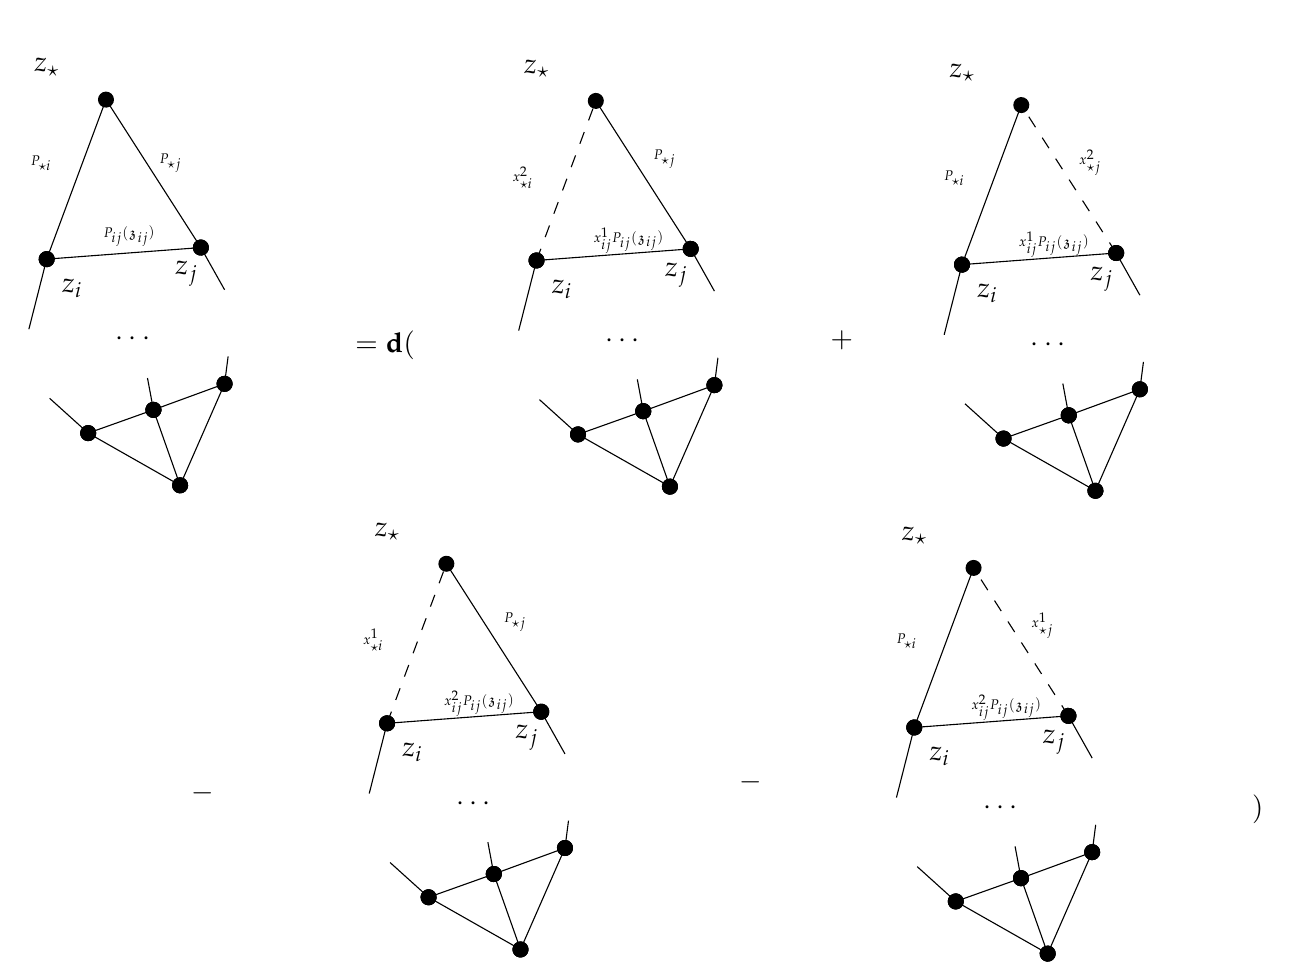
\begin{tikzpicture}[x=0.75pt,y=0.75pt,yscale=-1,xscale=1]
%uncomment if require: \path (0,468); %set diagram left start at 0, and has height of 468

%Straight Lines [id:da05577391005151622]
\draw    (45.67,112.69) -- (74.24,35.83) ;
\draw [shift={(74.24,35.83)}, rotate = 290.39] [color={rgb, 255:red, 0; green, 0; blue, 0 }  ][fill={rgb, 255:red, 0; green, 0; blue, 0 }  ][line width=0.75]      (0, 0) circle [x radius= 3.35, y radius= 3.35]   ;
\draw [shift={(45.67,112.69)}, rotate = 290.39] [color={rgb, 255:red, 0; green, 0; blue, 0 }  ][fill={rgb, 255:red, 0; green, 0; blue, 0 }  ][line width=0.75]      (0, 0) circle [x radius= 3.35, y radius= 3.35]   ;
%Straight Lines [id:da9941994376013314]
\draw    (119.95,107.11) -- (74.24,35.83) ;
\draw [shift={(119.95,107.11)}, rotate = 237.33] [color={rgb, 255:red, 0; green, 0; blue, 0 }  ][fill={rgb, 255:red, 0; green, 0; blue, 0 }  ][line width=0.75]      (0, 0) circle [x radius= 3.35, y radius= 3.35]   ;
%Straight Lines [id:da3900565594052461]
\draw    (109.95,221.66) -- (97.1,185.3) ;
\draw [shift={(97.1,185.3)}, rotate = 250.52] [color={rgb, 255:red, 0; green, 0; blue, 0 }  ][fill={rgb, 255:red, 0; green, 0; blue, 0 }  ][line width=0.75]      (0, 0) circle [x radius= 3.35, y radius= 3.35]   ;
\draw [shift={(109.95,221.66)}, rotate = 250.52] [color={rgb, 255:red, 0; green, 0; blue, 0 }  ][fill={rgb, 255:red, 0; green, 0; blue, 0 }  ][line width=0.75]      (0, 0) circle [x radius= 3.35, y radius= 3.35]   ;
%Straight Lines [id:da39495241281601645]
\draw    (119.95,107.11) -- (45.67,112.69) ;
\draw [shift={(45.67,112.69)}, rotate = 175.7] [color={rgb, 255:red, 0; green, 0; blue, 0 }  ][fill={rgb, 255:red, 0; green, 0; blue, 0 }  ][line width=0.75]      (0, 0) circle [x radius= 3.35, y radius= 3.35]   ;
\draw [shift={(119.95,107.11)}, rotate = 175.7] [color={rgb, 255:red, 0; green, 0; blue, 0 }  ][fill={rgb, 255:red, 0; green, 0; blue, 0 }  ][line width=0.75]      (0, 0) circle [x radius= 3.35, y radius= 3.35]   ;
%Straight Lines [id:da3458843670282836]
\draw    (65.67,196.51) -- (97.1,185.3) ;
\draw [shift={(97.1,185.3)}, rotate = 340.37] [color={rgb, 255:red, 0; green, 0; blue, 0 }  ][fill={rgb, 255:red, 0; green, 0; blue, 0 }  ][line width=0.75]      (0, 0) circle [x radius= 3.35, y radius= 3.35]   ;
\draw [shift={(65.67,196.51)}, rotate = 340.37] [color={rgb, 255:red, 0; green, 0; blue, 0 }  ][fill={rgb, 255:red, 0; green, 0; blue, 0 }  ][line width=0.75]      (0, 0) circle [x radius= 3.35, y radius= 3.35]   ;
%Straight Lines [id:da3629575229618873]
\draw    (65.67,196.51) -- (109.95,221.66) ;
\draw [shift={(109.95,221.66)}, rotate = 29.59] [color={rgb, 255:red, 0; green, 0; blue, 0 }  ][fill={rgb, 255:red, 0; green, 0; blue, 0 }  ][line width=0.75]      (0, 0) circle [x radius= 3.35, y radius= 3.35]   ;
\draw [shift={(65.67,196.51)}, rotate = 29.59] [color={rgb, 255:red, 0; green, 0; blue, 0 }  ][fill={rgb, 255:red, 0; green, 0; blue, 0 }  ][line width=0.75]      (0, 0) circle [x radius= 3.35, y radius= 3.35]   ;
%Straight Lines [id:da7374047900805547]
\draw    (45.67,112.69) -- (37.08,146.48) ;
\draw [shift={(45.67,112.69)}, rotate = 104.26] [color={rgb, 255:red, 0; green, 0; blue, 0 }  ][fill={rgb, 255:red, 0; green, 0; blue, 0 }  ][line width=0.75]      (0, 0) circle [x radius= 3.35, y radius= 3.35]   ;
%Straight Lines [id:da7354249192448576]
\draw    (119.95,107.11) -- (131.38,127.44) ;
\draw [shift={(119.95,107.11)}, rotate = 60.66] [color={rgb, 255:red, 0; green, 0; blue, 0 }  ][fill={rgb, 255:red, 0; green, 0; blue, 0 }  ][line width=0.75]      (0, 0) circle [x radius= 3.35, y radius= 3.35]   ;
%Straight Lines [id:da7512691918844618]
\draw    (97.1,185.3) -- (131.38,172.76) ;
\draw [shift={(131.38,172.76)}, rotate = 339.91] [color={rgb, 255:red, 0; green, 0; blue, 0 }  ][fill={rgb, 255:red, 0; green, 0; blue, 0 }  ][line width=0.75]      (0, 0) circle [x radius= 3.35, y radius= 3.35]   ;
\draw [shift={(97.1,185.3)}, rotate = 339.91] [color={rgb, 255:red, 0; green, 0; blue, 0 }  ][fill={rgb, 255:red, 0; green, 0; blue, 0 }  ][line width=0.75]      (0, 0) circle [x radius= 3.35, y radius= 3.35]   ;
%Straight Lines [id:da4433747900500091]
\draw    (65.67,196.51) -- (47.1,179.75) ;
\draw [shift={(65.67,196.51)}, rotate = 222.07] [color={rgb, 255:red, 0; green, 0; blue, 0 }  ][fill={rgb, 255:red, 0; green, 0; blue, 0 }  ][line width=0.75]      (0, 0) circle [x radius= 3.35, y radius= 3.35]   ;
%Straight Lines [id:da8725889104604558]
\draw    (97.1,185.3) -- (94.24,169.97) ;
\draw [shift={(97.1,185.3)}, rotate = 259.45] [color={rgb, 255:red, 0; green, 0; blue, 0 }  ][fill={rgb, 255:red, 0; green, 0; blue, 0 }  ][line width=0.75]      (0, 0) circle [x radius= 3.35, y radius= 3.35]   ;
%Straight Lines [id:da06318673435754363]
\draw    (131.38,172.76) -- (133.08,159.57) ;
\draw [shift={(131.38,172.76)}, rotate = 277.36] [color={rgb, 255:red, 0; green, 0; blue, 0 }  ][fill={rgb, 255:red, 0; green, 0; blue, 0 }  ][line width=0.75]      (0, 0) circle [x radius= 3.35, y radius= 3.35]   ;
%Straight Lines [id:da8635127857460636]
\draw    (109.95,221.66) -- (131.38,172.76) ;
\draw [shift={(131.38,172.76)}, rotate = 293.67] [color={rgb, 255:red, 0; green, 0; blue, 0 }  ][fill={rgb, 255:red, 0; green, 0; blue, 0 }  ][line width=0.75]      (0, 0) circle [x radius= 3.35, y radius= 3.35]   ;
\draw [shift={(109.95,221.66)}, rotate = 293.67] [color={rgb, 255:red, 0; green, 0; blue, 0 }  ][fill={rgb, 255:red, 0; green, 0; blue, 0 }  ][line width=0.75]      (0, 0) circle [x radius= 3.35, y radius= 3.35]   ;
%Straight Lines [id:da6079017959541106]
\draw  [dash pattern={on 4.5pt off 4.5pt}]  (281.67,113.33) -- (310.24,36.46) ;
\draw [shift={(310.24,36.46)}, rotate = 290.39] [color={rgb, 255:red, 0; green, 0; blue, 0 }  ][fill={rgb, 255:red, 0; green, 0; blue, 0 }  ][line width=0.75]      (0, 0) circle [x radius= 3.35, y radius= 3.35]   ;
\draw [shift={(281.67,113.33)}, rotate = 290.39] [color={rgb, 255:red, 0; green, 0; blue, 0 }  ][fill={rgb, 255:red, 0; green, 0; blue, 0 }  ][line width=0.75]      (0, 0) circle [x radius= 3.35, y radius= 3.35]   ;
%Straight Lines [id:da6262900974020484]
\draw    (355.95,107.74) -- (310.24,36.46) ;
\draw [shift={(355.95,107.74)}, rotate = 237.33] [color={rgb, 255:red, 0; green, 0; blue, 0 }  ][fill={rgb, 255:red, 0; green, 0; blue, 0 }  ][line width=0.75]      (0, 0) circle [x radius= 3.35, y radius= 3.35]   ;
%Straight Lines [id:da4207396882092873]
\draw    (345.95,222.29) -- (333.1,185.94) ;
\draw [shift={(333.1,185.94)}, rotate = 250.52] [color={rgb, 255:red, 0; green, 0; blue, 0 }  ][fill={rgb, 255:red, 0; green, 0; blue, 0 }  ][line width=0.75]      (0, 0) circle [x radius= 3.35, y radius= 3.35]   ;
\draw [shift={(345.95,222.29)}, rotate = 250.52] [color={rgb, 255:red, 0; green, 0; blue, 0 }  ][fill={rgb, 255:red, 0; green, 0; blue, 0 }  ][line width=0.75]      (0, 0) circle [x radius= 3.35, y radius= 3.35]   ;
%Straight Lines [id:da10130927807420287]
\draw    (355.95,107.74) -- (281.67,113.33) ;
\draw [shift={(281.67,113.33)}, rotate = 175.7] [color={rgb, 255:red, 0; green, 0; blue, 0 }  ][fill={rgb, 255:red, 0; green, 0; blue, 0 }  ][line width=0.75]      (0, 0) circle [x radius= 3.35, y radius= 3.35]   ;
\draw [shift={(355.95,107.74)}, rotate = 175.7] [color={rgb, 255:red, 0; green, 0; blue, 0 }  ][fill={rgb, 255:red, 0; green, 0; blue, 0 }  ][line width=0.75]      (0, 0) circle [x radius= 3.35, y radius= 3.35]   ;
%Straight Lines [id:da9973991574066416]
\draw    (301.67,197.14) -- (333.1,185.94) ;
\draw [shift={(333.1,185.94)}, rotate = 340.37] [color={rgb, 255:red, 0; green, 0; blue, 0 }  ][fill={rgb, 255:red, 0; green, 0; blue, 0 }  ][line width=0.75]      (0, 0) circle [x radius= 3.35, y radius= 3.35]   ;
\draw [shift={(301.67,197.14)}, rotate = 340.37] [color={rgb, 255:red, 0; green, 0; blue, 0 }  ][fill={rgb, 255:red, 0; green, 0; blue, 0 }  ][line width=0.75]      (0, 0) circle [x radius= 3.35, y radius= 3.35]   ;
%Straight Lines [id:da7208635053541128]
\draw    (301.67,197.14) -- (345.95,222.29) ;
\draw [shift={(345.95,222.29)}, rotate = 29.59] [color={rgb, 255:red, 0; green, 0; blue, 0 }  ][fill={rgb, 255:red, 0; green, 0; blue, 0 }  ][line width=0.75]      (0, 0) circle [x radius= 3.35, y radius= 3.35]   ;
\draw [shift={(301.67,197.14)}, rotate = 29.59] [color={rgb, 255:red, 0; green, 0; blue, 0 }  ][fill={rgb, 255:red, 0; green, 0; blue, 0 }  ][line width=0.75]      (0, 0) circle [x radius= 3.35, y radius= 3.35]   ;
%Straight Lines [id:da5476792808251072]
\draw    (281.67,113.33) -- (273.08,147.12) ;
\draw [shift={(281.67,113.33)}, rotate = 104.26] [color={rgb, 255:red, 0; green, 0; blue, 0 }  ][fill={rgb, 255:red, 0; green, 0; blue, 0 }  ][line width=0.75]      (0, 0) circle [x radius= 3.35, y radius= 3.35]   ;
%Straight Lines [id:da4842288863296871]
\draw    (355.95,107.74) -- (367.38,128.07) ;
\draw [shift={(355.95,107.74)}, rotate = 60.66] [color={rgb, 255:red, 0; green, 0; blue, 0 }  ][fill={rgb, 255:red, 0; green, 0; blue, 0 }  ][line width=0.75]      (0, 0) circle [x radius= 3.35, y radius= 3.35]   ;
%Straight Lines [id:da5181357205840986]
\draw    (333.1,185.94) -- (367.38,173.4) ;
\draw [shift={(367.38,173.4)}, rotate = 339.91] [color={rgb, 255:red, 0; green, 0; blue, 0 }  ][fill={rgb, 255:red, 0; green, 0; blue, 0 }  ][line width=0.75]      (0, 0) circle [x radius= 3.35, y radius= 3.35]   ;
\draw [shift={(333.1,185.94)}, rotate = 339.91] [color={rgb, 255:red, 0; green, 0; blue, 0 }  ][fill={rgb, 255:red, 0; green, 0; blue, 0 }  ][line width=0.75]      (0, 0) circle [x radius= 3.35, y radius= 3.35]   ;
%Straight Lines [id:da25998482008575174]
\draw    (301.67,197.14) -- (283.1,180.38) ;
\draw [shift={(301.67,197.14)}, rotate = 222.07] [color={rgb, 255:red, 0; green, 0; blue, 0 }  ][fill={rgb, 255:red, 0; green, 0; blue, 0 }  ][line width=0.75]      (0, 0) circle [x radius= 3.35, y radius= 3.35]   ;
%Straight Lines [id:da00593123197541745]
\draw    (333.1,185.94) -- (330.24,170.6) ;
\draw [shift={(333.1,185.94)}, rotate = 259.45] [color={rgb, 255:red, 0; green, 0; blue, 0 }  ][fill={rgb, 255:red, 0; green, 0; blue, 0 }  ][line width=0.75]      (0, 0) circle [x radius= 3.35, y radius= 3.35]   ;
%Straight Lines [id:da31696356189479014]
\draw    (367.38,173.4) -- (369.08,160.21) ;
\draw [shift={(367.38,173.4)}, rotate = 277.36] [color={rgb, 255:red, 0; green, 0; blue, 0 }  ][fill={rgb, 255:red, 0; green, 0; blue, 0 }  ][line width=0.75]      (0, 0) circle [x radius= 3.35, y radius= 3.35]   ;
%Straight Lines [id:da05067436226981181]
\draw    (345.95,222.29) -- (367.38,173.4) ;
\draw [shift={(367.38,173.4)}, rotate = 293.67] [color={rgb, 255:red, 0; green, 0; blue, 0 }  ][fill={rgb, 255:red, 0; green, 0; blue, 0 }  ][line width=0.75]      (0, 0) circle [x radius= 3.35, y radius= 3.35]   ;
\draw [shift={(345.95,222.29)}, rotate = 293.67] [color={rgb, 255:red, 0; green, 0; blue, 0 }  ][fill={rgb, 255:red, 0; green, 0; blue, 0 }  ][line width=0.75]      (0, 0) circle [x radius= 3.35, y radius= 3.35]   ;
%Straight Lines [id:da5379040559240473]
\draw  [dash pattern={on 4.5pt off 4.5pt}]  (209.67,336.33) -- (238.24,259.46) ;
\draw [shift={(238.24,259.46)}, rotate = 290.39] [color={rgb, 255:red, 0; green, 0; blue, 0 }  ][fill={rgb, 255:red, 0; green, 0; blue, 0 }  ][line width=0.75]      (0, 0) circle [x radius= 3.35, y radius= 3.35]   ;
\draw [shift={(209.67,336.33)}, rotate = 290.39] [color={rgb, 255:red, 0; green, 0; blue, 0 }  ][fill={rgb, 255:red, 0; green, 0; blue, 0 }  ][line width=0.75]      (0, 0) circle [x radius= 3.35, y radius= 3.35]   ;
%Straight Lines [id:da07964081672038281]
\draw    (283.95,330.74) -- (238.24,259.46) ;
\draw [shift={(283.95,330.74)}, rotate = 237.33] [color={rgb, 255:red, 0; green, 0; blue, 0 }  ][fill={rgb, 255:red, 0; green, 0; blue, 0 }  ][line width=0.75]      (0, 0) circle [x radius= 3.35, y radius= 3.35]   ;
%Straight Lines [id:da623421312454463]
\draw    (273.95,445.29) -- (261.1,408.94) ;
\draw [shift={(261.1,408.94)}, rotate = 250.52] [color={rgb, 255:red, 0; green, 0; blue, 0 }  ][fill={rgb, 255:red, 0; green, 0; blue, 0 }  ][line width=0.75]      (0, 0) circle [x radius= 3.35, y radius= 3.35]   ;
\draw [shift={(273.95,445.29)}, rotate = 250.52] [color={rgb, 255:red, 0; green, 0; blue, 0 }  ][fill={rgb, 255:red, 0; green, 0; blue, 0 }  ][line width=0.75]      (0, 0) circle [x radius= 3.35, y radius= 3.35]   ;
%Straight Lines [id:da12169856804436452]
\draw    (283.95,330.74) -- (209.67,336.33) ;
\draw [shift={(209.67,336.33)}, rotate = 175.7] [color={rgb, 255:red, 0; green, 0; blue, 0 }  ][fill={rgb, 255:red, 0; green, 0; blue, 0 }  ][line width=0.75]      (0, 0) circle [x radius= 3.35, y radius= 3.35]   ;
\draw [shift={(283.95,330.74)}, rotate = 175.7] [color={rgb, 255:red, 0; green, 0; blue, 0 }  ][fill={rgb, 255:red, 0; green, 0; blue, 0 }  ][line width=0.75]      (0, 0) circle [x radius= 3.35, y radius= 3.35]   ;
%Straight Lines [id:da9101675049165978]
\draw    (229.67,420.14) -- (261.1,408.94) ;
\draw [shift={(261.1,408.94)}, rotate = 340.37] [color={rgb, 255:red, 0; green, 0; blue, 0 }  ][fill={rgb, 255:red, 0; green, 0; blue, 0 }  ][line width=0.75]      (0, 0) circle [x radius= 3.35, y radius= 3.35]   ;
\draw [shift={(229.67,420.14)}, rotate = 340.37] [color={rgb, 255:red, 0; green, 0; blue, 0 }  ][fill={rgb, 255:red, 0; green, 0; blue, 0 }  ][line width=0.75]      (0, 0) circle [x radius= 3.35, y radius= 3.35]   ;
%Straight Lines [id:da043757079672652965]
\draw    (229.67,420.14) -- (273.95,445.29) ;
\draw [shift={(273.95,445.29)}, rotate = 29.59] [color={rgb, 255:red, 0; green, 0; blue, 0 }  ][fill={rgb, 255:red, 0; green, 0; blue, 0 }  ][line width=0.75]      (0, 0) circle [x radius= 3.35, y radius= 3.35]   ;
\draw [shift={(229.67,420.14)}, rotate = 29.59] [color={rgb, 255:red, 0; green, 0; blue, 0 }  ][fill={rgb, 255:red, 0; green, 0; blue, 0 }  ][line width=0.75]      (0, 0) circle [x radius= 3.35, y radius= 3.35]   ;
%Straight Lines [id:da3984530587665718]
\draw    (209.67,336.33) -- (201.08,370.12) ;
\draw [shift={(209.67,336.33)}, rotate = 104.26] [color={rgb, 255:red, 0; green, 0; blue, 0 }  ][fill={rgb, 255:red, 0; green, 0; blue, 0 }  ][line width=0.75]      (0, 0) circle [x radius= 3.35, y radius= 3.35]   ;
%Straight Lines [id:da3646360861208682]
\draw    (283.95,330.74) -- (295.38,351.07) ;
\draw [shift={(283.95,330.74)}, rotate = 60.66] [color={rgb, 255:red, 0; green, 0; blue, 0 }  ][fill={rgb, 255:red, 0; green, 0; blue, 0 }  ][line width=0.75]      (0, 0) circle [x radius= 3.35, y radius= 3.35]   ;
%Straight Lines [id:da004765418535702004]
\draw    (261.1,408.94) -- (295.38,396.4) ;
\draw [shift={(295.38,396.4)}, rotate = 339.91] [color={rgb, 255:red, 0; green, 0; blue, 0 }  ][fill={rgb, 255:red, 0; green, 0; blue, 0 }  ][line width=0.75]      (0, 0) circle [x radius= 3.35, y radius= 3.35]   ;
\draw [shift={(261.1,408.94)}, rotate = 339.91] [color={rgb, 255:red, 0; green, 0; blue, 0 }  ][fill={rgb, 255:red, 0; green, 0; blue, 0 }  ][line width=0.75]      (0, 0) circle [x radius= 3.35, y radius= 3.35]   ;
%Straight Lines [id:da4471076941500518]
\draw    (229.67,420.14) -- (211.1,403.38) ;
\draw [shift={(229.67,420.14)}, rotate = 222.07] [color={rgb, 255:red, 0; green, 0; blue, 0 }  ][fill={rgb, 255:red, 0; green, 0; blue, 0 }  ][line width=0.75]      (0, 0) circle [x radius= 3.35, y radius= 3.35]   ;
%Straight Lines [id:da8892260272577963]
\draw    (261.1,408.94) -- (258.24,393.6) ;
\draw [shift={(261.1,408.94)}, rotate = 259.45] [color={rgb, 255:red, 0; green, 0; blue, 0 }  ][fill={rgb, 255:red, 0; green, 0; blue, 0 }  ][line width=0.75]      (0, 0) circle [x radius= 3.35, y radius= 3.35]   ;
%Straight Lines [id:da5366908426898191]
\draw    (295.38,396.4) -- (297.08,383.21) ;
\draw [shift={(295.38,396.4)}, rotate = 277.36] [color={rgb, 255:red, 0; green, 0; blue, 0 }  ][fill={rgb, 255:red, 0; green, 0; blue, 0 }  ][line width=0.75]      (0, 0) circle [x radius= 3.35, y radius= 3.35]   ;
%Straight Lines [id:da6406878003707261]
\draw    (273.95,445.29) -- (295.38,396.4) ;
\draw [shift={(295.38,396.4)}, rotate = 293.67] [color={rgb, 255:red, 0; green, 0; blue, 0 }  ][fill={rgb, 255:red, 0; green, 0; blue, 0 }  ][line width=0.75]      (0, 0) circle [x radius= 3.35, y radius= 3.35]   ;
\draw [shift={(273.95,445.29)}, rotate = 293.67] [color={rgb, 255:red, 0; green, 0; blue, 0 }  ][fill={rgb, 255:red, 0; green, 0; blue, 0 }  ][line width=0.75]      (0, 0) circle [x radius= 3.35, y radius= 3.35]   ;
%Straight Lines [id:da02022332446143138]
\draw    (486.67,115.33) -- (515.24,38.46) ;
\draw [shift={(515.24,38.46)}, rotate = 290.39] [color={rgb, 255:red, 0; green, 0; blue, 0 }  ][fill={rgb, 255:red, 0; green, 0; blue, 0 }  ][line width=0.75]      (0, 0) circle [x radius= 3.35, y radius= 3.35]   ;
\draw [shift={(486.67,115.33)}, rotate = 290.39] [color={rgb, 255:red, 0; green, 0; blue, 0 }  ][fill={rgb, 255:red, 0; green, 0; blue, 0 }  ][line width=0.75]      (0, 0) circle [x radius= 3.35, y radius= 3.35]   ;
%Straight Lines [id:da5288571741275976]
\draw  [dash pattern={on 4.5pt off 4.5pt}]  (560.95,109.74) -- (515.24,38.46) ;
\draw [shift={(560.95,109.74)}, rotate = 237.33] [color={rgb, 255:red, 0; green, 0; blue, 0 }  ][fill={rgb, 255:red, 0; green, 0; blue, 0 }  ][line width=0.75]      (0, 0) circle [x radius= 3.35, y radius= 3.35]   ;
%Straight Lines [id:da5128746037479821]
\draw    (550.95,224.29) -- (538.1,187.94) ;
\draw [shift={(538.1,187.94)}, rotate = 250.52] [color={rgb, 255:red, 0; green, 0; blue, 0 }  ][fill={rgb, 255:red, 0; green, 0; blue, 0 }  ][line width=0.75]      (0, 0) circle [x radius= 3.35, y radius= 3.35]   ;
\draw [shift={(550.95,224.29)}, rotate = 250.52] [color={rgb, 255:red, 0; green, 0; blue, 0 }  ][fill={rgb, 255:red, 0; green, 0; blue, 0 }  ][line width=0.75]      (0, 0) circle [x radius= 3.35, y radius= 3.35]   ;
%Straight Lines [id:da6140123126224639]
\draw    (560.95,109.74) -- (486.67,115.33) ;
\draw [shift={(486.67,115.33)}, rotate = 175.7] [color={rgb, 255:red, 0; green, 0; blue, 0 }  ][fill={rgb, 255:red, 0; green, 0; blue, 0 }  ][line width=0.75]      (0, 0) circle [x radius= 3.35, y radius= 3.35]   ;
\draw [shift={(560.95,109.74)}, rotate = 175.7] [color={rgb, 255:red, 0; green, 0; blue, 0 }  ][fill={rgb, 255:red, 0; green, 0; blue, 0 }  ][line width=0.75]      (0, 0) circle [x radius= 3.35, y radius= 3.35]   ;
%Straight Lines [id:da7457563432649676]
\draw    (506.67,199.14) -- (538.1,187.94) ;
\draw [shift={(538.1,187.94)}, rotate = 340.37] [color={rgb, 255:red, 0; green, 0; blue, 0 }  ][fill={rgb, 255:red, 0; green, 0; blue, 0 }  ][line width=0.75]      (0, 0) circle [x radius= 3.35, y radius= 3.35]   ;
\draw [shift={(506.67,199.14)}, rotate = 340.37] [color={rgb, 255:red, 0; green, 0; blue, 0 }  ][fill={rgb, 255:red, 0; green, 0; blue, 0 }  ][line width=0.75]      (0, 0) circle [x radius= 3.35, y radius= 3.35]   ;
%Straight Lines [id:da537605841830689]
\draw    (506.67,199.14) -- (550.95,224.29) ;
\draw [shift={(550.95,224.29)}, rotate = 29.59] [color={rgb, 255:red, 0; green, 0; blue, 0 }  ][fill={rgb, 255:red, 0; green, 0; blue, 0 }  ][line width=0.75]      (0, 0) circle [x radius= 3.35, y radius= 3.35]   ;
\draw [shift={(506.67,199.14)}, rotate = 29.59] [color={rgb, 255:red, 0; green, 0; blue, 0 }  ][fill={rgb, 255:red, 0; green, 0; blue, 0 }  ][line width=0.75]      (0, 0) circle [x radius= 3.35, y radius= 3.35]   ;
%Straight Lines [id:da8002140501405561]
\draw    (486.67,115.33) -- (478.08,149.12) ;
\draw [shift={(486.67,115.33)}, rotate = 104.26] [color={rgb, 255:red, 0; green, 0; blue, 0 }  ][fill={rgb, 255:red, 0; green, 0; blue, 0 }  ][line width=0.75]      (0, 0) circle [x radius= 3.35, y radius= 3.35]   ;
%Straight Lines [id:da5909286524354338]
\draw    (560.95,109.74) -- (572.38,130.07) ;
\draw [shift={(560.95,109.74)}, rotate = 60.66] [color={rgb, 255:red, 0; green, 0; blue, 0 }  ][fill={rgb, 255:red, 0; green, 0; blue, 0 }  ][line width=0.75]      (0, 0) circle [x radius= 3.35, y radius= 3.35]   ;
%Straight Lines [id:da8937326368583083]
\draw    (538.1,187.94) -- (572.38,175.4) ;
\draw [shift={(572.38,175.4)}, rotate = 339.91] [color={rgb, 255:red, 0; green, 0; blue, 0 }  ][fill={rgb, 255:red, 0; green, 0; blue, 0 }  ][line width=0.75]      (0, 0) circle [x radius= 3.35, y radius= 3.35]   ;
\draw [shift={(538.1,187.94)}, rotate = 339.91] [color={rgb, 255:red, 0; green, 0; blue, 0 }  ][fill={rgb, 255:red, 0; green, 0; blue, 0 }  ][line width=0.75]      (0, 0) circle [x radius= 3.35, y radius= 3.35]   ;
%Straight Lines [id:da39486850360585657]
\draw    (506.67,199.14) -- (488.1,182.38) ;
\draw [shift={(506.67,199.14)}, rotate = 222.07] [color={rgb, 255:red, 0; green, 0; blue, 0 }  ][fill={rgb, 255:red, 0; green, 0; blue, 0 }  ][line width=0.75]      (0, 0) circle [x radius= 3.35, y radius= 3.35]   ;
%Straight Lines [id:da5723040194124529]
\draw    (538.1,187.94) -- (535.24,172.6) ;
\draw [shift={(538.1,187.94)}, rotate = 259.45] [color={rgb, 255:red, 0; green, 0; blue, 0 }  ][fill={rgb, 255:red, 0; green, 0; blue, 0 }  ][line width=0.75]      (0, 0) circle [x radius= 3.35, y radius= 3.35]   ;
%Straight Lines [id:da6617379630684848]
\draw    (572.38,175.4) -- (574.08,162.21) ;
\draw [shift={(572.38,175.4)}, rotate = 277.36] [color={rgb, 255:red, 0; green, 0; blue, 0 }  ][fill={rgb, 255:red, 0; green, 0; blue, 0 }  ][line width=0.75]      (0, 0) circle [x radius= 3.35, y radius= 3.35]   ;
%Straight Lines [id:da06155672117733357]
\draw    (550.95,224.29) -- (572.38,175.4) ;
\draw [shift={(572.38,175.4)}, rotate = 293.67] [color={rgb, 255:red, 0; green, 0; blue, 0 }  ][fill={rgb, 255:red, 0; green, 0; blue, 0 }  ][line width=0.75]      (0, 0) circle [x radius= 3.35, y radius= 3.35]   ;
\draw [shift={(550.95,224.29)}, rotate = 293.67] [color={rgb, 255:red, 0; green, 0; blue, 0 }  ][fill={rgb, 255:red, 0; green, 0; blue, 0 }  ][line width=0.75]      (0, 0) circle [x radius= 3.35, y radius= 3.35]   ;
%Straight Lines [id:da26570006292245996]
\draw    (463.67,338.33) -- (492.24,261.46) ;
\draw [shift={(492.24,261.46)}, rotate = 290.39] [color={rgb, 255:red, 0; green, 0; blue, 0 }  ][fill={rgb, 255:red, 0; green, 0; blue, 0 }  ][line width=0.75]      (0, 0) circle [x radius= 3.35, y radius= 3.35]   ;
\draw [shift={(463.67,338.33)}, rotate = 290.39] [color={rgb, 255:red, 0; green, 0; blue, 0 }  ][fill={rgb, 255:red, 0; green, 0; blue, 0 }  ][line width=0.75]      (0, 0) circle [x radius= 3.35, y radius= 3.35]   ;
%Straight Lines [id:da40306180015380066]
\draw  [dash pattern={on 4.5pt off 4.5pt}]  (537.95,332.74) -- (492.24,261.46) ;
\draw [shift={(537.95,332.74)}, rotate = 237.33] [color={rgb, 255:red, 0; green, 0; blue, 0 }  ][fill={rgb, 255:red, 0; green, 0; blue, 0 }  ][line width=0.75]      (0, 0) circle [x radius= 3.35, y radius= 3.35]   ;
%Straight Lines [id:da18554926508633796]
\draw    (527.95,447.29) -- (515.1,410.94) ;
\draw [shift={(515.1,410.94)}, rotate = 250.52] [color={rgb, 255:red, 0; green, 0; blue, 0 }  ][fill={rgb, 255:red, 0; green, 0; blue, 0 }  ][line width=0.75]      (0, 0) circle [x radius= 3.35, y radius= 3.35]   ;
\draw [shift={(527.95,447.29)}, rotate = 250.52] [color={rgb, 255:red, 0; green, 0; blue, 0 }  ][fill={rgb, 255:red, 0; green, 0; blue, 0 }  ][line width=0.75]      (0, 0) circle [x radius= 3.35, y radius= 3.35]   ;
%Straight Lines [id:da40858047037677103]
\draw    (537.95,332.74) -- (463.67,338.33) ;
\draw [shift={(463.67,338.33)}, rotate = 175.7] [color={rgb, 255:red, 0; green, 0; blue, 0 }  ][fill={rgb, 255:red, 0; green, 0; blue, 0 }  ][line width=0.75]      (0, 0) circle [x radius= 3.35, y radius= 3.35]   ;
\draw [shift={(537.95,332.74)}, rotate = 175.7] [color={rgb, 255:red, 0; green, 0; blue, 0 }  ][fill={rgb, 255:red, 0; green, 0; blue, 0 }  ][line width=0.75]      (0, 0) circle [x radius= 3.35, y radius= 3.35]   ;
%Straight Lines [id:da7743038002276321]
\draw    (483.67,422.14) -- (515.1,410.94) ;
\draw [shift={(515.1,410.94)}, rotate = 340.37] [color={rgb, 255:red, 0; green, 0; blue, 0 }  ][fill={rgb, 255:red, 0; green, 0; blue, 0 }  ][line width=0.75]      (0, 0) circle [x radius= 3.35, y radius= 3.35]   ;
\draw [shift={(483.67,422.14)}, rotate = 340.37] [color={rgb, 255:red, 0; green, 0; blue, 0 }  ][fill={rgb, 255:red, 0; green, 0; blue, 0 }  ][line width=0.75]      (0, 0) circle [x radius= 3.35, y radius= 3.35]   ;
%Straight Lines [id:da43373975235177076]
\draw    (483.67,422.14) -- (527.95,447.29) ;
\draw [shift={(527.95,447.29)}, rotate = 29.59] [color={rgb, 255:red, 0; green, 0; blue, 0 }  ][fill={rgb, 255:red, 0; green, 0; blue, 0 }  ][line width=0.75]      (0, 0) circle [x radius= 3.35, y radius= 3.35]   ;
\draw [shift={(483.67,422.14)}, rotate = 29.59] [color={rgb, 255:red, 0; green, 0; blue, 0 }  ][fill={rgb, 255:red, 0; green, 0; blue, 0 }  ][line width=0.75]      (0, 0) circle [x radius= 3.35, y radius= 3.35]   ;
%Straight Lines [id:da059421258991678716]
\draw    (463.67,338.33) -- (455.08,372.12) ;
\draw [shift={(463.67,338.33)}, rotate = 104.26] [color={rgb, 255:red, 0; green, 0; blue, 0 }  ][fill={rgb, 255:red, 0; green, 0; blue, 0 }  ][line width=0.75]      (0, 0) circle [x radius= 3.35, y radius= 3.35]   ;
%Straight Lines [id:da9003970058401041]
\draw    (537.95,332.74) -- (549.38,353.07) ;
\draw [shift={(537.95,332.74)}, rotate = 60.66] [color={rgb, 255:red, 0; green, 0; blue, 0 }  ][fill={rgb, 255:red, 0; green, 0; blue, 0 }  ][line width=0.75]      (0, 0) circle [x radius= 3.35, y radius= 3.35]   ;
%Straight Lines [id:da7049527604866348]
\draw    (515.1,410.94) -- (549.38,398.4) ;
\draw [shift={(549.38,398.4)}, rotate = 339.91] [color={rgb, 255:red, 0; green, 0; blue, 0 }  ][fill={rgb, 255:red, 0; green, 0; blue, 0 }  ][line width=0.75]      (0, 0) circle [x radius= 3.35, y radius= 3.35]   ;
\draw [shift={(515.1,410.94)}, rotate = 339.91] [color={rgb, 255:red, 0; green, 0; blue, 0 }  ][fill={rgb, 255:red, 0; green, 0; blue, 0 }  ][line width=0.75]      (0, 0) circle [x radius= 3.35, y radius= 3.35]   ;
%Straight Lines [id:da30853022450967305]
\draw    (483.67,422.14) -- (465.1,405.38) ;
\draw [shift={(483.67,422.14)}, rotate = 222.07] [color={rgb, 255:red, 0; green, 0; blue, 0 }  ][fill={rgb, 255:red, 0; green, 0; blue, 0 }  ][line width=0.75]      (0, 0) circle [x radius= 3.35, y radius= 3.35]   ;
%Straight Lines [id:da8152787882036101]
\draw    (515.1,410.94) -- (512.24,395.6) ;
\draw [shift={(515.1,410.94)}, rotate = 259.45] [color={rgb, 255:red, 0; green, 0; blue, 0 }  ][fill={rgb, 255:red, 0; green, 0; blue, 0 }  ][line width=0.75]      (0, 0) circle [x radius= 3.35, y radius= 3.35]   ;
%Straight Lines [id:da5978237424415016]
\draw    (549.38,398.4) -- (551.08,385.21) ;
\draw [shift={(549.38,398.4)}, rotate = 277.36] [color={rgb, 255:red, 0; green, 0; blue, 0 }  ][fill={rgb, 255:red, 0; green, 0; blue, 0 }  ][line width=0.75]      (0, 0) circle [x radius= 3.35, y radius= 3.35]   ;
%Straight Lines [id:da6023515255937397]
\draw    (527.95,447.29) -- (549.38,398.4) ;
\draw [shift={(549.38,398.4)}, rotate = 293.67] [color={rgb, 255:red, 0; green, 0; blue, 0 }  ][fill={rgb, 255:red, 0; green, 0; blue, 0 }  ][line width=0.75]      (0, 0) circle [x radius= 3.35, y radius= 3.35]   ;
\draw [shift={(527.95,447.29)}, rotate = 293.67] [color={rgb, 255:red, 0; green, 0; blue, 0 }  ][fill={rgb, 255:red, 0; green, 0; blue, 0 }  ][line width=0.75]      (0, 0) circle [x radius= 3.35, y radius= 3.35]   ;

% Text Node
\draw (38.19,14.77) node [anchor=north west][inner sep=0.75pt]    {$z_{\star }$};
% Text Node
\draw (106.1,112.48) node [anchor=north west][inner sep=0.75pt]    {$z_{j}{}$};
% Text Node
\draw (51.53,120.86) node [anchor=north west][inner sep=0.75pt]    {$z_{i}$};
% Text Node
\draw (77.48,147.08) node [anchor=north west][inner sep=0.75pt]    {$\cdots $};
% Text Node
\draw (71.78,95.9) node [anchor=north west][inner sep=0.75pt]  [font=\tiny,rotate=-359.06]  {$P_{ij}(\mathfrak{z}_{ij})$};
% Text Node
\draw (192.98,145.94) node [anchor=north west][inner sep=0.75pt]    {$=\mathbf{d}($};
% Text Node
\draw (274.19,15.4) node [anchor=north west][inner sep=0.75pt]    {$z_{\star }$};
% Text Node
\draw (342.1,113.11) node [anchor=north west][inner sep=0.75pt]    {$z_{j}{}$};
% Text Node
\draw (287.53,121.49) node [anchor=north west][inner sep=0.75pt]    {$z_{i}$};
% Text Node
\draw (313.48,147.71) node [anchor=north west][inner sep=0.75pt]    {$\cdots $};
% Text Node
\draw (307.78,96.54) node [anchor=north west][inner sep=0.75pt]  [font=\tiny,rotate=-359.06]  {$x_{ij}^{1} P_{ij}(\mathfrak{z}_{ij})$};
% Text Node
\draw (36.78,61.9) node [anchor=north west][inner sep=0.75pt]  [font=\tiny,rotate=-359.06]  {$P_{\star i}$};
% Text Node
\draw (98.78,60.9) node [anchor=north west][inner sep=0.75pt]  [font=\tiny,rotate=-359.06]  {$P_{\star j}$};
% Text Node
\draw (268.78,66.9) node [anchor=north west][inner sep=0.75pt]  [font=\tiny,rotate=-359.06]  {$x_{\star i}^{2}$};
% Text Node
\draw (336.78,58.9) node [anchor=north west][inner sep=0.75pt]  [font=\tiny,rotate=-359.06]  {$P_{\star j}$};
% Text Node
\draw (421.98,145.94) node [anchor=north west][inner sep=0.75pt]    {$+$};
% Text Node
\draw (202.19,238.4) node [anchor=north west][inner sep=0.75pt]    {$z_{\star }$};
% Text Node
\draw (270.1,336.11) node [anchor=north west][inner sep=0.75pt]    {$z_{j}{}$};
% Text Node
\draw (215.53,344.49) node [anchor=north west][inner sep=0.75pt]    {$z_{i}$};
% Text Node
\draw (241.48,370.71) node [anchor=north west][inner sep=0.75pt]    {$\cdots $};
% Text Node
\draw (235.78,319.54) node [anchor=north west][inner sep=0.75pt]  [font=\tiny,rotate=-359.06]  {$x_{ij}^{2} P_{ij}(\mathfrak{z}_{ij})$};
% Text Node
\draw (196.78,289.9) node [anchor=north west][inner sep=0.75pt]  [font=\tiny,rotate=-359.06]  {$x_{\star i}^{1}$};
% Text Node
\draw (264.78,281.9) node [anchor=north west][inner sep=0.75pt]  [font=\tiny,rotate=-359.06]  {$P_{\star j}$};
% Text Node
\draw (113.98,363.94) node [anchor=north west][inner sep=0.75pt]    {$-$};
% Text Node
\draw (479.19,17.4) node [anchor=north west][inner sep=0.75pt]    {$z_{\star }$};
% Text Node
\draw (547.1,115.11) node [anchor=north west][inner sep=0.75pt]    {$z_{j}{}$};
% Text Node
\draw (492.53,123.49) node [anchor=north west][inner sep=0.75pt]    {$z_{i}$};
% Text Node
\draw (518.48,149.71) node [anchor=north west][inner sep=0.75pt]    {$\cdots $};
% Text Node
\draw (512.78,98.54) node [anchor=north west][inner sep=0.75pt]  [font=\tiny,rotate=-359.06]  {$x_{ij}^{1} P_{ij}(\mathfrak{z}_{ij})$};
% Text Node
\draw (541.78,58.9) node [anchor=north west][inner sep=0.75pt]  [font=\tiny,rotate=-359.06]  {$x_{\star j}^{2}$};
% Text Node
\draw (476.78,68.9) node [anchor=north west][inner sep=0.75pt]  [font=\tiny,rotate=-359.06]  {$P_{\star i}$};
% Text Node
\draw (377.98,358.94) node [anchor=north west][inner sep=0.75pt]    {$-$};
% Text Node
\draw (456.19,240.4) node [anchor=north west][inner sep=0.75pt]    {$z_{\star }$};
% Text Node
\draw (524.1,338.11) node [anchor=north west][inner sep=0.75pt]    {$z_{j}{}$};
% Text Node
\draw (469.53,346.49) node [anchor=north west][inner sep=0.75pt]    {$z_{i}$};
% Text Node
\draw (495.48,372.71) node [anchor=north west][inner sep=0.75pt]    {$\cdots $};
% Text Node
\draw (489.78,321.54) node [anchor=north west][inner sep=0.75pt]  [font=\tiny,rotate=-359.06]  {$x_{ij}^{2} P_{ij}(\mathfrak{z}_{ij})$};
% Text Node
\draw (518.78,281.9) node [anchor=north west][inner sep=0.75pt]  [font=\tiny,rotate=-359.06]  {$x_{\star j}^{1}$};
% Text Node
\draw (453.78,291.9) node [anchor=north west][inner sep=0.75pt]  [font=\tiny,rotate=-359.06]  {$P_{\star i}$};
% Text Node
\draw (625,369.4) node [anchor=north west][inner sep=0.75pt]    {$)$};


\end{tikzpicture}
  \caption{}\label{}
\end{figure}
\begin{figure}[htp]
  \centering


\tikzset{every picture/.style={line width=0.75pt}} %set default line width to 0.75pt

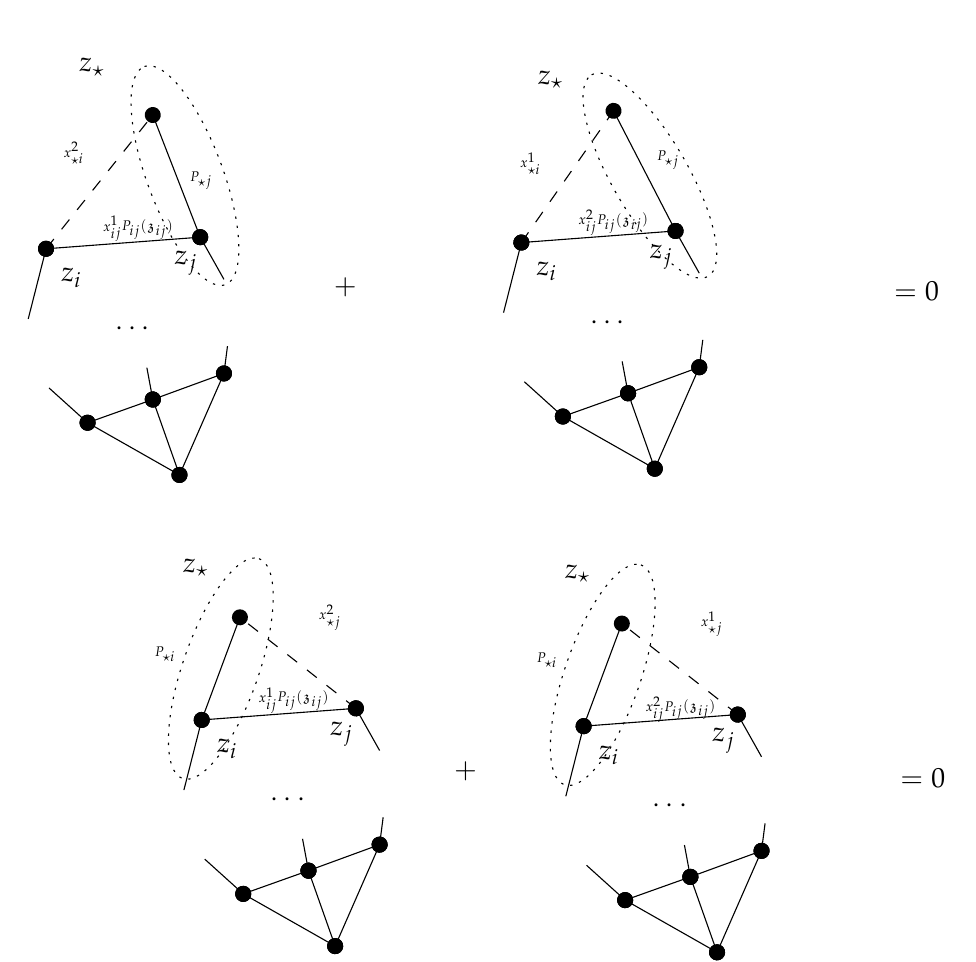
\begin{tikzpicture}[x=0.75pt,y=0.75pt,yscale=-1,xscale=1]
%uncomment if require: \path (0,499); %set diagram left start at 0, and has height of 499

%Straight Lines [id:da016701861550822983]
\draw  [dash pattern={on 4.5pt off 4.5pt}]  (49.67,112.33) -- (101.08,47.88) ;
\draw [shift={(101.08,47.88)}, rotate = 308.58] [color={rgb, 255:red, 0; green, 0; blue, 0 }  ][fill={rgb, 255:red, 0; green, 0; blue, 0 }  ][line width=0.75]      (0, 0) circle [x radius= 3.35, y radius= 3.35]   ;
\draw [shift={(49.67,112.33)}, rotate = 308.58] [color={rgb, 255:red, 0; green, 0; blue, 0 }  ][fill={rgb, 255:red, 0; green, 0; blue, 0 }  ][line width=0.75]      (0, 0) circle [x radius= 3.35, y radius= 3.35]   ;
%Straight Lines [id:da6673420184100265]
\draw    (123.95,106.74) -- (101.08,47.88) ;
\draw [shift={(123.95,106.74)}, rotate = 248.77] [color={rgb, 255:red, 0; green, 0; blue, 0 }  ][fill={rgb, 255:red, 0; green, 0; blue, 0 }  ][line width=0.75]      (0, 0) circle [x radius= 3.35, y radius= 3.35]   ;
%Straight Lines [id:da291545258927024]
\draw    (113.95,221.29) -- (101.1,184.94) ;
\draw [shift={(101.1,184.94)}, rotate = 250.52] [color={rgb, 255:red, 0; green, 0; blue, 0 }  ][fill={rgb, 255:red, 0; green, 0; blue, 0 }  ][line width=0.75]      (0, 0) circle [x radius= 3.35, y radius= 3.35]   ;
\draw [shift={(113.95,221.29)}, rotate = 250.52] [color={rgb, 255:red, 0; green, 0; blue, 0 }  ][fill={rgb, 255:red, 0; green, 0; blue, 0 }  ][line width=0.75]      (0, 0) circle [x radius= 3.35, y radius= 3.35]   ;
%Straight Lines [id:da30577453142010946]
\draw    (123.95,106.74) -- (49.67,112.33) ;
\draw [shift={(49.67,112.33)}, rotate = 175.7] [color={rgb, 255:red, 0; green, 0; blue, 0 }  ][fill={rgb, 255:red, 0; green, 0; blue, 0 }  ][line width=0.75]      (0, 0) circle [x radius= 3.35, y radius= 3.35]   ;
\draw [shift={(123.95,106.74)}, rotate = 175.7] [color={rgb, 255:red, 0; green, 0; blue, 0 }  ][fill={rgb, 255:red, 0; green, 0; blue, 0 }  ][line width=0.75]      (0, 0) circle [x radius= 3.35, y radius= 3.35]   ;
%Straight Lines [id:da3313498870535505]
\draw    (69.67,196.14) -- (101.1,184.94) ;
\draw [shift={(101.1,184.94)}, rotate = 340.37] [color={rgb, 255:red, 0; green, 0; blue, 0 }  ][fill={rgb, 255:red, 0; green, 0; blue, 0 }  ][line width=0.75]      (0, 0) circle [x radius= 3.35, y radius= 3.35]   ;
\draw [shift={(69.67,196.14)}, rotate = 340.37] [color={rgb, 255:red, 0; green, 0; blue, 0 }  ][fill={rgb, 255:red, 0; green, 0; blue, 0 }  ][line width=0.75]      (0, 0) circle [x radius= 3.35, y radius= 3.35]   ;
%Straight Lines [id:da299261848456837]
\draw    (69.67,196.14) -- (113.95,221.29) ;
\draw [shift={(113.95,221.29)}, rotate = 29.59] [color={rgb, 255:red, 0; green, 0; blue, 0 }  ][fill={rgb, 255:red, 0; green, 0; blue, 0 }  ][line width=0.75]      (0, 0) circle [x radius= 3.35, y radius= 3.35]   ;
\draw [shift={(69.67,196.14)}, rotate = 29.59] [color={rgb, 255:red, 0; green, 0; blue, 0 }  ][fill={rgb, 255:red, 0; green, 0; blue, 0 }  ][line width=0.75]      (0, 0) circle [x radius= 3.35, y radius= 3.35]   ;
%Straight Lines [id:da9810894594549351]
\draw    (49.67,112.33) -- (41.08,146.12) ;
\draw [shift={(49.67,112.33)}, rotate = 104.26] [color={rgb, 255:red, 0; green, 0; blue, 0 }  ][fill={rgb, 255:red, 0; green, 0; blue, 0 }  ][line width=0.75]      (0, 0) circle [x radius= 3.35, y radius= 3.35]   ;
%Straight Lines [id:da12287886848281349]
\draw    (123.95,106.74) -- (135.38,127.07) ;
\draw [shift={(123.95,106.74)}, rotate = 60.66] [color={rgb, 255:red, 0; green, 0; blue, 0 }  ][fill={rgb, 255:red, 0; green, 0; blue, 0 }  ][line width=0.75]      (0, 0) circle [x radius= 3.35, y radius= 3.35]   ;
%Straight Lines [id:da682096516134622]
\draw    (101.1,184.94) -- (135.38,172.4) ;
\draw [shift={(135.38,172.4)}, rotate = 339.91] [color={rgb, 255:red, 0; green, 0; blue, 0 }  ][fill={rgb, 255:red, 0; green, 0; blue, 0 }  ][line width=0.75]      (0, 0) circle [x radius= 3.35, y radius= 3.35]   ;
\draw [shift={(101.1,184.94)}, rotate = 339.91] [color={rgb, 255:red, 0; green, 0; blue, 0 }  ][fill={rgb, 255:red, 0; green, 0; blue, 0 }  ][line width=0.75]      (0, 0) circle [x radius= 3.35, y radius= 3.35]   ;
%Straight Lines [id:da6856933973629049]
\draw    (69.67,196.14) -- (51.1,179.38) ;
\draw [shift={(69.67,196.14)}, rotate = 222.07] [color={rgb, 255:red, 0; green, 0; blue, 0 }  ][fill={rgb, 255:red, 0; green, 0; blue, 0 }  ][line width=0.75]      (0, 0) circle [x radius= 3.35, y radius= 3.35]   ;
%Straight Lines [id:da2006582255893108]
\draw    (101.1,184.94) -- (98.24,169.6) ;
\draw [shift={(101.1,184.94)}, rotate = 259.45] [color={rgb, 255:red, 0; green, 0; blue, 0 }  ][fill={rgb, 255:red, 0; green, 0; blue, 0 }  ][line width=0.75]      (0, 0) circle [x radius= 3.35, y radius= 3.35]   ;
%Straight Lines [id:da6590264087471263]
\draw    (135.38,172.4) -- (137.08,159.21) ;
\draw [shift={(135.38,172.4)}, rotate = 277.36] [color={rgb, 255:red, 0; green, 0; blue, 0 }  ][fill={rgb, 255:red, 0; green, 0; blue, 0 }  ][line width=0.75]      (0, 0) circle [x radius= 3.35, y radius= 3.35]   ;
%Straight Lines [id:da34426877079033824]
\draw    (113.95,221.29) -- (135.38,172.4) ;
\draw [shift={(135.38,172.4)}, rotate = 293.67] [color={rgb, 255:red, 0; green, 0; blue, 0 }  ][fill={rgb, 255:red, 0; green, 0; blue, 0 }  ][line width=0.75]      (0, 0) circle [x radius= 3.35, y radius= 3.35]   ;
\draw [shift={(113.95,221.29)}, rotate = 293.67] [color={rgb, 255:red, 0; green, 0; blue, 0 }  ][fill={rgb, 255:red, 0; green, 0; blue, 0 }  ][line width=0.75]      (0, 0) circle [x radius= 3.35, y radius= 3.35]   ;
%Straight Lines [id:da7372440454354685]
\draw  [dash pattern={on 4.5pt off 4.5pt}]  (278.67,109.33) -- (323.08,45.88) ;
\draw [shift={(323.08,45.88)}, rotate = 304.99] [color={rgb, 255:red, 0; green, 0; blue, 0 }  ][fill={rgb, 255:red, 0; green, 0; blue, 0 }  ][line width=0.75]      (0, 0) circle [x radius= 3.35, y radius= 3.35]   ;
\draw [shift={(278.67,109.33)}, rotate = 304.99] [color={rgb, 255:red, 0; green, 0; blue, 0 }  ][fill={rgb, 255:red, 0; green, 0; blue, 0 }  ][line width=0.75]      (0, 0) circle [x radius= 3.35, y radius= 3.35]   ;
%Straight Lines [id:da2825766414379851]
\draw    (352.95,103.74) -- (323.08,45.88) ;
\draw [shift={(352.95,103.74)}, rotate = 242.69] [color={rgb, 255:red, 0; green, 0; blue, 0 }  ][fill={rgb, 255:red, 0; green, 0; blue, 0 }  ][line width=0.75]      (0, 0) circle [x radius= 3.35, y radius= 3.35]   ;
%Straight Lines [id:da40167171611659924]
\draw    (342.95,218.29) -- (330.1,181.94) ;
\draw [shift={(330.1,181.94)}, rotate = 250.52] [color={rgb, 255:red, 0; green, 0; blue, 0 }  ][fill={rgb, 255:red, 0; green, 0; blue, 0 }  ][line width=0.75]      (0, 0) circle [x radius= 3.35, y radius= 3.35]   ;
\draw [shift={(342.95,218.29)}, rotate = 250.52] [color={rgb, 255:red, 0; green, 0; blue, 0 }  ][fill={rgb, 255:red, 0; green, 0; blue, 0 }  ][line width=0.75]      (0, 0) circle [x radius= 3.35, y radius= 3.35]   ;
%Straight Lines [id:da3991150002283752]
\draw    (352.95,103.74) -- (278.67,109.33) ;
\draw [shift={(278.67,109.33)}, rotate = 175.7] [color={rgb, 255:red, 0; green, 0; blue, 0 }  ][fill={rgb, 255:red, 0; green, 0; blue, 0 }  ][line width=0.75]      (0, 0) circle [x radius= 3.35, y radius= 3.35]   ;
\draw [shift={(352.95,103.74)}, rotate = 175.7] [color={rgb, 255:red, 0; green, 0; blue, 0 }  ][fill={rgb, 255:red, 0; green, 0; blue, 0 }  ][line width=0.75]      (0, 0) circle [x radius= 3.35, y radius= 3.35]   ;
%Straight Lines [id:da4636329963381429]
\draw    (298.67,193.14) -- (330.1,181.94) ;
\draw [shift={(330.1,181.94)}, rotate = 340.37] [color={rgb, 255:red, 0; green, 0; blue, 0 }  ][fill={rgb, 255:red, 0; green, 0; blue, 0 }  ][line width=0.75]      (0, 0) circle [x radius= 3.35, y radius= 3.35]   ;
\draw [shift={(298.67,193.14)}, rotate = 340.37] [color={rgb, 255:red, 0; green, 0; blue, 0 }  ][fill={rgb, 255:red, 0; green, 0; blue, 0 }  ][line width=0.75]      (0, 0) circle [x radius= 3.35, y radius= 3.35]   ;
%Straight Lines [id:da9296126353581244]
\draw    (298.67,193.14) -- (342.95,218.29) ;
\draw [shift={(342.95,218.29)}, rotate = 29.59] [color={rgb, 255:red, 0; green, 0; blue, 0 }  ][fill={rgb, 255:red, 0; green, 0; blue, 0 }  ][line width=0.75]      (0, 0) circle [x radius= 3.35, y radius= 3.35]   ;
\draw [shift={(298.67,193.14)}, rotate = 29.59] [color={rgb, 255:red, 0; green, 0; blue, 0 }  ][fill={rgb, 255:red, 0; green, 0; blue, 0 }  ][line width=0.75]      (0, 0) circle [x radius= 3.35, y radius= 3.35]   ;
%Straight Lines [id:da8095525896445261]
\draw    (278.67,109.33) -- (270.08,143.12) ;
\draw [shift={(278.67,109.33)}, rotate = 104.26] [color={rgb, 255:red, 0; green, 0; blue, 0 }  ][fill={rgb, 255:red, 0; green, 0; blue, 0 }  ][line width=0.75]      (0, 0) circle [x radius= 3.35, y radius= 3.35]   ;
%Straight Lines [id:da8280296256933743]
\draw    (352.95,103.74) -- (364.38,124.07) ;
\draw [shift={(352.95,103.74)}, rotate = 60.66] [color={rgb, 255:red, 0; green, 0; blue, 0 }  ][fill={rgb, 255:red, 0; green, 0; blue, 0 }  ][line width=0.75]      (0, 0) circle [x radius= 3.35, y radius= 3.35]   ;
%Straight Lines [id:da21586336732017686]
\draw    (330.1,181.94) -- (364.38,169.4) ;
\draw [shift={(364.38,169.4)}, rotate = 339.91] [color={rgb, 255:red, 0; green, 0; blue, 0 }  ][fill={rgb, 255:red, 0; green, 0; blue, 0 }  ][line width=0.75]      (0, 0) circle [x radius= 3.35, y radius= 3.35]   ;
\draw [shift={(330.1,181.94)}, rotate = 339.91] [color={rgb, 255:red, 0; green, 0; blue, 0 }  ][fill={rgb, 255:red, 0; green, 0; blue, 0 }  ][line width=0.75]      (0, 0) circle [x radius= 3.35, y radius= 3.35]   ;
%Straight Lines [id:da7620376533304356]
\draw    (298.67,193.14) -- (280.1,176.38) ;
\draw [shift={(298.67,193.14)}, rotate = 222.07] [color={rgb, 255:red, 0; green, 0; blue, 0 }  ][fill={rgb, 255:red, 0; green, 0; blue, 0 }  ][line width=0.75]      (0, 0) circle [x radius= 3.35, y radius= 3.35]   ;
%Straight Lines [id:da593740390455542]
\draw    (330.1,181.94) -- (327.24,166.6) ;
\draw [shift={(330.1,181.94)}, rotate = 259.45] [color={rgb, 255:red, 0; green, 0; blue, 0 }  ][fill={rgb, 255:red, 0; green, 0; blue, 0 }  ][line width=0.75]      (0, 0) circle [x radius= 3.35, y radius= 3.35]   ;
%Straight Lines [id:da39315643175806314]
\draw    (364.38,169.4) -- (366.08,156.21) ;
\draw [shift={(364.38,169.4)}, rotate = 277.36] [color={rgb, 255:red, 0; green, 0; blue, 0 }  ][fill={rgb, 255:red, 0; green, 0; blue, 0 }  ][line width=0.75]      (0, 0) circle [x radius= 3.35, y radius= 3.35]   ;
%Straight Lines [id:da32162649978428925]
\draw    (342.95,218.29) -- (364.38,169.4) ;
\draw [shift={(364.38,169.4)}, rotate = 293.67] [color={rgb, 255:red, 0; green, 0; blue, 0 }  ][fill={rgb, 255:red, 0; green, 0; blue, 0 }  ][line width=0.75]      (0, 0) circle [x radius= 3.35, y radius= 3.35]   ;
\draw [shift={(342.95,218.29)}, rotate = 293.67] [color={rgb, 255:red, 0; green, 0; blue, 0 }  ][fill={rgb, 255:red, 0; green, 0; blue, 0 }  ][line width=0.75]      (0, 0) circle [x radius= 3.35, y radius= 3.35]   ;
%Straight Lines [id:da3032317735841781]
\draw    (124.67,339.33) -- (143.08,289.88) ;
\draw [shift={(143.08,289.88)}, rotate = 290.42] [color={rgb, 255:red, 0; green, 0; blue, 0 }  ][fill={rgb, 255:red, 0; green, 0; blue, 0 }  ][line width=0.75]      (0, 0) circle [x radius= 3.35, y radius= 3.35]   ;
\draw [shift={(124.67,339.33)}, rotate = 290.42] [color={rgb, 255:red, 0; green, 0; blue, 0 }  ][fill={rgb, 255:red, 0; green, 0; blue, 0 }  ][line width=0.75]      (0, 0) circle [x radius= 3.35, y radius= 3.35]   ;
%Straight Lines [id:da3474375340285918]
\draw  [dash pattern={on 4.5pt off 4.5pt}]  (198.95,333.74) -- (143.08,289.88) ;
\draw [shift={(198.95,333.74)}, rotate = 218.13] [color={rgb, 255:red, 0; green, 0; blue, 0 }  ][fill={rgb, 255:red, 0; green, 0; blue, 0 }  ][line width=0.75]      (0, 0) circle [x radius= 3.35, y radius= 3.35]   ;
%Straight Lines [id:da165277748890025]
\draw    (188.95,448.29) -- (176.1,411.94) ;
\draw [shift={(176.1,411.94)}, rotate = 250.52] [color={rgb, 255:red, 0; green, 0; blue, 0 }  ][fill={rgb, 255:red, 0; green, 0; blue, 0 }  ][line width=0.75]      (0, 0) circle [x radius= 3.35, y radius= 3.35]   ;
\draw [shift={(188.95,448.29)}, rotate = 250.52] [color={rgb, 255:red, 0; green, 0; blue, 0 }  ][fill={rgb, 255:red, 0; green, 0; blue, 0 }  ][line width=0.75]      (0, 0) circle [x radius= 3.35, y radius= 3.35]   ;
%Straight Lines [id:da397412668453182]
\draw    (198.95,333.74) -- (124.67,339.33) ;
\draw [shift={(124.67,339.33)}, rotate = 175.7] [color={rgb, 255:red, 0; green, 0; blue, 0 }  ][fill={rgb, 255:red, 0; green, 0; blue, 0 }  ][line width=0.75]      (0, 0) circle [x radius= 3.35, y radius= 3.35]   ;
\draw [shift={(198.95,333.74)}, rotate = 175.7] [color={rgb, 255:red, 0; green, 0; blue, 0 }  ][fill={rgb, 255:red, 0; green, 0; blue, 0 }  ][line width=0.75]      (0, 0) circle [x radius= 3.35, y radius= 3.35]   ;
%Straight Lines [id:da44938459851536394]
\draw    (144.67,423.14) -- (176.1,411.94) ;
\draw [shift={(176.1,411.94)}, rotate = 340.37] [color={rgb, 255:red, 0; green, 0; blue, 0 }  ][fill={rgb, 255:red, 0; green, 0; blue, 0 }  ][line width=0.75]      (0, 0) circle [x radius= 3.35, y radius= 3.35]   ;
\draw [shift={(144.67,423.14)}, rotate = 340.37] [color={rgb, 255:red, 0; green, 0; blue, 0 }  ][fill={rgb, 255:red, 0; green, 0; blue, 0 }  ][line width=0.75]      (0, 0) circle [x radius= 3.35, y radius= 3.35]   ;
%Straight Lines [id:da3704675773059698]
\draw    (144.67,423.14) -- (188.95,448.29) ;
\draw [shift={(188.95,448.29)}, rotate = 29.59] [color={rgb, 255:red, 0; green, 0; blue, 0 }  ][fill={rgb, 255:red, 0; green, 0; blue, 0 }  ][line width=0.75]      (0, 0) circle [x radius= 3.35, y radius= 3.35]   ;
\draw [shift={(144.67,423.14)}, rotate = 29.59] [color={rgb, 255:red, 0; green, 0; blue, 0 }  ][fill={rgb, 255:red, 0; green, 0; blue, 0 }  ][line width=0.75]      (0, 0) circle [x radius= 3.35, y radius= 3.35]   ;
%Straight Lines [id:da48205725415781386]
\draw    (124.67,339.33) -- (116.08,373.12) ;
\draw [shift={(124.67,339.33)}, rotate = 104.26] [color={rgb, 255:red, 0; green, 0; blue, 0 }  ][fill={rgb, 255:red, 0; green, 0; blue, 0 }  ][line width=0.75]      (0, 0) circle [x radius= 3.35, y radius= 3.35]   ;
%Straight Lines [id:da9315082783753994]
\draw    (198.95,333.74) -- (210.38,354.07) ;
\draw [shift={(198.95,333.74)}, rotate = 60.66] [color={rgb, 255:red, 0; green, 0; blue, 0 }  ][fill={rgb, 255:red, 0; green, 0; blue, 0 }  ][line width=0.75]      (0, 0) circle [x radius= 3.35, y radius= 3.35]   ;
%Straight Lines [id:da362339232985051]
\draw    (176.1,411.94) -- (210.38,399.4) ;
\draw [shift={(210.38,399.4)}, rotate = 339.91] [color={rgb, 255:red, 0; green, 0; blue, 0 }  ][fill={rgb, 255:red, 0; green, 0; blue, 0 }  ][line width=0.75]      (0, 0) circle [x radius= 3.35, y radius= 3.35]   ;
\draw [shift={(176.1,411.94)}, rotate = 339.91] [color={rgb, 255:red, 0; green, 0; blue, 0 }  ][fill={rgb, 255:red, 0; green, 0; blue, 0 }  ][line width=0.75]      (0, 0) circle [x radius= 3.35, y radius= 3.35]   ;
%Straight Lines [id:da6388701280697504]
\draw    (144.67,423.14) -- (126.1,406.38) ;
\draw [shift={(144.67,423.14)}, rotate = 222.07] [color={rgb, 255:red, 0; green, 0; blue, 0 }  ][fill={rgb, 255:red, 0; green, 0; blue, 0 }  ][line width=0.75]      (0, 0) circle [x radius= 3.35, y radius= 3.35]   ;
%Straight Lines [id:da4393981169899286]
\draw    (176.1,411.94) -- (173.24,396.6) ;
\draw [shift={(176.1,411.94)}, rotate = 259.45] [color={rgb, 255:red, 0; green, 0; blue, 0 }  ][fill={rgb, 255:red, 0; green, 0; blue, 0 }  ][line width=0.75]      (0, 0) circle [x radius= 3.35, y radius= 3.35]   ;
%Straight Lines [id:da7727675541044259]
\draw    (210.38,399.4) -- (212.08,386.21) ;
\draw [shift={(210.38,399.4)}, rotate = 277.36] [color={rgb, 255:red, 0; green, 0; blue, 0 }  ][fill={rgb, 255:red, 0; green, 0; blue, 0 }  ][line width=0.75]      (0, 0) circle [x radius= 3.35, y radius= 3.35]   ;
%Straight Lines [id:da8732431429179641]
\draw    (188.95,448.29) -- (210.38,399.4) ;
\draw [shift={(210.38,399.4)}, rotate = 293.67] [color={rgb, 255:red, 0; green, 0; blue, 0 }  ][fill={rgb, 255:red, 0; green, 0; blue, 0 }  ][line width=0.75]      (0, 0) circle [x radius= 3.35, y radius= 3.35]   ;
\draw [shift={(188.95,448.29)}, rotate = 293.67] [color={rgb, 255:red, 0; green, 0; blue, 0 }  ][fill={rgb, 255:red, 0; green, 0; blue, 0 }  ][line width=0.75]      (0, 0) circle [x radius= 3.35, y radius= 3.35]   ;
%Shape: Ellipse [id:dp054723026974621725]
\draw  [dash pattern={on 0.84pt off 2.51pt}] (312.54,28.49) .. controls (321.28,23.44) and (340.93,41.1) .. (356.41,67.93) .. controls (371.9,94.76) and (377.37,120.6) .. (368.63,125.65) .. controls (359.89,130.69) and (340.24,113.04) .. (324.75,86.21) .. controls (309.26,59.38) and (303.8,33.54) .. (312.54,28.49) -- cycle ;
%Shape: Ellipse [id:dp5426866590205677]
\draw  [dash pattern={on 0.84pt off 2.51pt}] (97.07,24.48) .. controls (106.53,20.97) and (122.94,41.67) .. (133.72,70.71) .. controls (144.5,99.75) and (145.56,126.15) .. (136.1,129.66) .. controls (126.64,133.17) and (110.23,112.47) .. (99.45,83.43) .. controls (88.67,54.39) and (87.6,27.99) .. (97.07,24.48) -- cycle ;
%Shape: Ellipse [id:dp8432340335804664]
\draw  [dash pattern={on 0.84pt off 2.51pt}] (152.29,261.62) .. controls (161.82,264.93) and (161.31,291.34) .. (151.14,320.61) .. controls (140.98,349.87) and (125,370.9) .. (115.47,367.59) .. controls (105.93,364.28) and (106.44,337.87) .. (116.61,308.61) .. controls (126.78,279.34) and (142.75,258.31) .. (152.29,261.62) -- cycle ;
%Straight Lines [id:da1625791202902105]
\draw    (308.67,342.33) -- (327.08,292.88) ;
\draw [shift={(327.08,292.88)}, rotate = 290.42] [color={rgb, 255:red, 0; green, 0; blue, 0 }  ][fill={rgb, 255:red, 0; green, 0; blue, 0 }  ][line width=0.75]      (0, 0) circle [x radius= 3.35, y radius= 3.35]   ;
\draw [shift={(308.67,342.33)}, rotate = 290.42] [color={rgb, 255:red, 0; green, 0; blue, 0 }  ][fill={rgb, 255:red, 0; green, 0; blue, 0 }  ][line width=0.75]      (0, 0) circle [x radius= 3.35, y radius= 3.35]   ;
%Straight Lines [id:da746432742696095]
\draw  [dash pattern={on 4.5pt off 4.5pt}]  (382.95,336.74) -- (327.08,292.88) ;
\draw [shift={(382.95,336.74)}, rotate = 218.13] [color={rgb, 255:red, 0; green, 0; blue, 0 }  ][fill={rgb, 255:red, 0; green, 0; blue, 0 }  ][line width=0.75]      (0, 0) circle [x radius= 3.35, y radius= 3.35]   ;
%Straight Lines [id:da17219373332834387]
\draw    (372.95,451.29) -- (360.1,414.94) ;
\draw [shift={(360.1,414.94)}, rotate = 250.52] [color={rgb, 255:red, 0; green, 0; blue, 0 }  ][fill={rgb, 255:red, 0; green, 0; blue, 0 }  ][line width=0.75]      (0, 0) circle [x radius= 3.35, y radius= 3.35]   ;
\draw [shift={(372.95,451.29)}, rotate = 250.52] [color={rgb, 255:red, 0; green, 0; blue, 0 }  ][fill={rgb, 255:red, 0; green, 0; blue, 0 }  ][line width=0.75]      (0, 0) circle [x radius= 3.35, y radius= 3.35]   ;
%Straight Lines [id:da4621347064619983]
\draw    (382.95,336.74) -- (308.67,342.33) ;
\draw [shift={(308.67,342.33)}, rotate = 175.7] [color={rgb, 255:red, 0; green, 0; blue, 0 }  ][fill={rgb, 255:red, 0; green, 0; blue, 0 }  ][line width=0.75]      (0, 0) circle [x radius= 3.35, y radius= 3.35]   ;
\draw [shift={(382.95,336.74)}, rotate = 175.7] [color={rgb, 255:red, 0; green, 0; blue, 0 }  ][fill={rgb, 255:red, 0; green, 0; blue, 0 }  ][line width=0.75]      (0, 0) circle [x radius= 3.35, y radius= 3.35]   ;
%Straight Lines [id:da23173002946728105]
\draw    (328.67,426.14) -- (360.1,414.94) ;
\draw [shift={(360.1,414.94)}, rotate = 340.37] [color={rgb, 255:red, 0; green, 0; blue, 0 }  ][fill={rgb, 255:red, 0; green, 0; blue, 0 }  ][line width=0.75]      (0, 0) circle [x radius= 3.35, y radius= 3.35]   ;
\draw [shift={(328.67,426.14)}, rotate = 340.37] [color={rgb, 255:red, 0; green, 0; blue, 0 }  ][fill={rgb, 255:red, 0; green, 0; blue, 0 }  ][line width=0.75]      (0, 0) circle [x radius= 3.35, y radius= 3.35]   ;
%Straight Lines [id:da5632624463997629]
\draw    (328.67,426.14) -- (372.95,451.29) ;
\draw [shift={(372.95,451.29)}, rotate = 29.59] [color={rgb, 255:red, 0; green, 0; blue, 0 }  ][fill={rgb, 255:red, 0; green, 0; blue, 0 }  ][line width=0.75]      (0, 0) circle [x radius= 3.35, y radius= 3.35]   ;
\draw [shift={(328.67,426.14)}, rotate = 29.59] [color={rgb, 255:red, 0; green, 0; blue, 0 }  ][fill={rgb, 255:red, 0; green, 0; blue, 0 }  ][line width=0.75]      (0, 0) circle [x radius= 3.35, y radius= 3.35]   ;
%Straight Lines [id:da6318864871870671]
\draw    (308.67,342.33) -- (300.08,376.12) ;
\draw [shift={(308.67,342.33)}, rotate = 104.26] [color={rgb, 255:red, 0; green, 0; blue, 0 }  ][fill={rgb, 255:red, 0; green, 0; blue, 0 }  ][line width=0.75]      (0, 0) circle [x radius= 3.35, y radius= 3.35]   ;
%Straight Lines [id:da17370773737391154]
\draw    (382.95,336.74) -- (394.38,357.07) ;
\draw [shift={(382.95,336.74)}, rotate = 60.66] [color={rgb, 255:red, 0; green, 0; blue, 0 }  ][fill={rgb, 255:red, 0; green, 0; blue, 0 }  ][line width=0.75]      (0, 0) circle [x radius= 3.35, y radius= 3.35]   ;
%Straight Lines [id:da9219816290172171]
\draw    (360.1,414.94) -- (394.38,402.4) ;
\draw [shift={(394.38,402.4)}, rotate = 339.91] [color={rgb, 255:red, 0; green, 0; blue, 0 }  ][fill={rgb, 255:red, 0; green, 0; blue, 0 }  ][line width=0.75]      (0, 0) circle [x radius= 3.35, y radius= 3.35]   ;
\draw [shift={(360.1,414.94)}, rotate = 339.91] [color={rgb, 255:red, 0; green, 0; blue, 0 }  ][fill={rgb, 255:red, 0; green, 0; blue, 0 }  ][line width=0.75]      (0, 0) circle [x radius= 3.35, y radius= 3.35]   ;
%Straight Lines [id:da4744650663960672]
\draw    (328.67,426.14) -- (310.1,409.38) ;
\draw [shift={(328.67,426.14)}, rotate = 222.07] [color={rgb, 255:red, 0; green, 0; blue, 0 }  ][fill={rgb, 255:red, 0; green, 0; blue, 0 }  ][line width=0.75]      (0, 0) circle [x radius= 3.35, y radius= 3.35]   ;
%Straight Lines [id:da023175902953707084]
\draw    (360.1,414.94) -- (357.24,399.6) ;
\draw [shift={(360.1,414.94)}, rotate = 259.45] [color={rgb, 255:red, 0; green, 0; blue, 0 }  ][fill={rgb, 255:red, 0; green, 0; blue, 0 }  ][line width=0.75]      (0, 0) circle [x radius= 3.35, y radius= 3.35]   ;
%Straight Lines [id:da6229829657306729]
\draw    (394.38,402.4) -- (396.08,389.21) ;
\draw [shift={(394.38,402.4)}, rotate = 277.36] [color={rgb, 255:red, 0; green, 0; blue, 0 }  ][fill={rgb, 255:red, 0; green, 0; blue, 0 }  ][line width=0.75]      (0, 0) circle [x radius= 3.35, y radius= 3.35]   ;
%Straight Lines [id:da23553498408248252]
\draw    (372.95,451.29) -- (394.38,402.4) ;
\draw [shift={(394.38,402.4)}, rotate = 293.67] [color={rgb, 255:red, 0; green, 0; blue, 0 }  ][fill={rgb, 255:red, 0; green, 0; blue, 0 }  ][line width=0.75]      (0, 0) circle [x radius= 3.35, y radius= 3.35]   ;
\draw [shift={(372.95,451.29)}, rotate = 293.67] [color={rgb, 255:red, 0; green, 0; blue, 0 }  ][fill={rgb, 255:red, 0; green, 0; blue, 0 }  ][line width=0.75]      (0, 0) circle [x radius= 3.35, y radius= 3.35]   ;
%Shape: Ellipse [id:dp9089413040928458]
\draw  [dash pattern={on 0.84pt off 2.51pt}] (336.29,264.62) .. controls (345.82,267.93) and (345.31,294.34) .. (335.14,323.61) .. controls (324.98,352.87) and (309,373.9) .. (299.47,370.59) .. controls (289.93,367.28) and (290.44,340.87) .. (300.61,311.61) .. controls (310.78,282.34) and (326.75,261.31) .. (336.29,264.62) -- cycle ;

% Text Node
\draw (456.98,126.94) node [anchor=north west][inner sep=0.75pt]    {$=0$};
% Text Node
\draw (64.19,19.4) node [anchor=north west][inner sep=0.75pt]    {$z_{\star }$};
% Text Node
\draw (110.1,112.11) node [anchor=north west][inner sep=0.75pt]    {$z_{j}{}$};
% Text Node
\draw (55.53,120.49) node [anchor=north west][inner sep=0.75pt]    {$z_{i}$};
% Text Node
\draw (81.48,146.71) node [anchor=north west][inner sep=0.75pt]    {$\cdots $};
% Text Node
\draw (75.78,95.54) node [anchor=north west][inner sep=0.75pt]  [font=\tiny,rotate=-359.06]  {$x_{ij}^{1} P_{ij}(\mathfrak{z}_{ij})$};
% Text Node
\draw (56.78,59.9) node [anchor=north west][inner sep=0.75pt]  [font=\tiny,rotate=-359.06]  {$x_{\star i}^{2}$};
% Text Node
\draw (117.78,73.9) node [anchor=north west][inner sep=0.75pt]  [font=\tiny,rotate=-359.06]  {$P_{\star j}$};
% Text Node
\draw (186.98,124.94) node [anchor=north west][inner sep=0.75pt]    {$+$};
% Text Node
\draw (285.19,25.4) node [anchor=north west][inner sep=0.75pt]    {$z_{\star }$};
% Text Node
\draw (339.1,109.11) node [anchor=north west][inner sep=0.75pt]    {$z_{j}{}$};
% Text Node
\draw (284.53,117.49) node [anchor=north west][inner sep=0.75pt]    {$z_{i}$};
% Text Node
\draw (310.48,143.71) node [anchor=north west][inner sep=0.75pt]    {$\cdots $};
% Text Node
\draw (304.78,92.54) node [anchor=north west][inner sep=0.75pt]  [font=\tiny,rotate=-359.06]  {$x_{ij}^{2} P_{ij}(\mathfrak{z}_{ij})$};
% Text Node
\draw (276.78,64.9) node [anchor=north west][inner sep=0.75pt]  [font=\tiny,rotate=-359.06]  {$x_{\star i}^{1}$};
% Text Node
\draw (342.78,63.9) node [anchor=north west][inner sep=0.75pt]  [font=\tiny,rotate=-359.06]  {$P_{\star j}$};
% Text Node
\draw (114.19,260.4) node [anchor=north west][inner sep=0.75pt]    {$z_{\star }$};
% Text Node
\draw (185.1,339.11) node [anchor=north west][inner sep=0.75pt]    {$z_{j}{}$};
% Text Node
\draw (130.53,347.49) node [anchor=north west][inner sep=0.75pt]    {$z_{i}$};
% Text Node
\draw (156.48,373.71) node [anchor=north west][inner sep=0.75pt]    {$\cdots $};
% Text Node
\draw (150.78,322.54) node [anchor=north west][inner sep=0.75pt]  [font=\tiny,rotate=-359.06]  {$x_{ij}^{1} P_{ij}(\mathfrak{z}_{ij})$};
% Text Node
\draw (179.78,282.9) node [anchor=north west][inner sep=0.75pt]  [font=\tiny,rotate=-359.06]  {$x_{\star j}^{2}$};
% Text Node
\draw (100.78,302.9) node [anchor=north west][inner sep=0.75pt]  [font=\tiny,rotate=-359.06]  {$P_{\star i}$};
% Text Node
\draw (244.98,357.94) node [anchor=north west][inner sep=0.75pt]    {$+$};
% Text Node
\draw (460,361.4) node [anchor=north west][inner sep=0.75pt]    {$=0$};
% Text Node
\draw (298.19,263.4) node [anchor=north west][inner sep=0.75pt]    {$z_{\star }$};
% Text Node
\draw (369.1,342.11) node [anchor=north west][inner sep=0.75pt]    {$z_{j}{}$};
% Text Node
\draw (314.53,350.49) node [anchor=north west][inner sep=0.75pt]    {$z_{i}$};
% Text Node
\draw (340.48,376.71) node [anchor=north west][inner sep=0.75pt]    {$\cdots $};
% Text Node
\draw (337.2,326.97) node [anchor=north west][inner sep=0.75pt]  [font=\tiny,rotate=-359.06]  {$x_{ij}^{2} P_{ij}(\mathfrak{z}_{ij})$};
% Text Node
\draw (363.78,285.9) node [anchor=north west][inner sep=0.75pt]  [font=\tiny,rotate=-359.06]  {$x_{\star j}^{1}$};
% Text Node
\draw (284.78,305.9) node [anchor=north west][inner sep=0.75pt]  [font=\tiny,rotate=-359.06]  {$P_{\star i}$};


\end{tikzpicture}
  \caption{}\label{}
\end{figure}
We first notice that

\begin{align*}
\mu_{\{1\dots n\star\}}\left(W_{\Gamma^{\star}}(\mathfrak{z}_{e})\right)   &=\mu_{\{1\dots n\star\}}\left(W_{\Gamma}(\mathfrak{z}_{e})\cdot P_{\star i}(\mathfrak{z}_{\star i})P_{\star j}(\mathfrak{z}_{\star j})\right)     \\
   & =\mu_{\{1\dots n\star\}}\left(W_{\Gamma}(\tilde{\mathfrak{z}}_{e})\cdot P_{\star i}P_{\star j}\right)\cdot e^{(\lambda_i|\mathfrak{z}_{i\star})+(\lambda_j|\mathfrak{z}_{j\star})}
\end{align*}
here
$$
\begin{cases}
\tilde{\mathfrak{z}}_e=\mathfrak{z}_e+\mathfrak{z}_{\star i}  , & \mbox{if } i\in V(e),e\neq ij, \\
\tilde{\mathfrak{z}}_e=\mathfrak{z}_e+\mathfrak{z}_{\star j}  , & \mbox{if } j\in V(e),e\neq ij,\\
\tilde{\mathfrak{z}}_e=\mathfrak{z}_e-\mathfrak{z}_{\star i}-\mathfrak{z}_{\star j}   , &  \mbox{if} e=ij,\\
\tilde{\mathfrak{z}}_e=\mathfrak{z}_e  , & \mbox{otherwise}.
\end{cases}
$$
Using Lemma \ref{RecursiveLemma}, we have
$$
  P_{\star i}P_{\star j}P_{ij}(\tilde{\mathfrak{z}}_{ij})=\mathbf{d}\left(P_{ij}(\tilde{\mathfrak{z}}_{ij})P_{\star j}\cdot x_{\star i}\wedge x_{ij}+P_{ij}(\tilde{\mathfrak{z}}_{ij})P_{\star i}\cdot x_{\star j}\wedge x_{ij}\right)
$$
Then
\begin{align*}
  \mu_{\{1\dots n\star\}}\left(W_{\Gamma}(\tilde{\mathfrak{z}}_{e})\cdot P_{\star i}P_{\star j}\right) &=\mu_{\{1\dots n\star\}}\left(\mathbf{d}\left(W_{\Gamma}(\tilde{\mathfrak{z}}_{e})P_{\star j}\cdot x_{\star i}\wedge x_{ij}+W_{\Gamma}(\tilde{\mathfrak{z}}_{e})P_{\star i}\cdot x_{\star j}\wedge x_{ij}\right)\right)  \\
   &= \mu_{\{\star\bullet\}}\circ \mu_{\{1\dots n\}}\left(W_{\Gamma}(\tilde{\mathfrak{z}}_{e})\cdot (x_{ij}\wedge x_{\star j})P_{\star i }\right)+\mu_{\{\star\bullet\}}\circ \mu_{\{1\dots n\}}\left(W_{\Gamma}(\tilde{\mathfrak{z}}_{e})\cdot (x_{ij}\wedge x_{\star i})P_{\star j}\right)\\
   &+ \underbrace{ \mu_{\{1\dots n\}}\circ\mu_{\{\star i\}}\left(W_{\Gamma}(\tilde{\mathfrak{z}}_{e})\cdot (x_{ij}\wedge x_{\star j})P_{\star i }\right)}_{=0}+\underbrace{\mu_{\{1\dots n\}}\circ\mu_{\{\star j\}}\left(W_{\Gamma}(\tilde{\mathfrak{z}}_{e})\cdot (x_{ij}\wedge x_{\star i})P_{\star j}\right)}_{0}.
\end{align*}
We will prove a stronger statement by induction. In fact, we will prove that
$$
 \sum_{\vec{e},v\in \vec{e}} \partial_{\mathfrak{z}_{\vec{e}}}  \mathbf{W}^{r,s}_{\Gamma,\mathbf{H}(o,e)}=-\lambda_v.
$$
\begin{align*}
   &  \mathbf{W}^{r,s}_{\Gamma,\mathbf{H}(o,e)}(\lambda;\dots,r_{\star}\tilde{\mathfrak{z}}_{ij},\dots)\\
   & =\mathbf{W}^{r,s}_{\Gamma,\mathbf{H}(o,e)}(\lambda;\tilde{\mathfrak{z}}_{\vec{e}})-(1-r_{\star})\left(\partial_{\mathfrak{z}_{ij}}\mathbf{W}^{r,s}_{\Gamma,\mathbf{H}(o,e)}(\lambda;{\mathfrak{z}}_{\vec{e}})|\tilde{\mathfrak{z}}_{ij}\right)\\
   &=\mathbf{W}^{r,s}_{\Gamma,\mathbf{H}(o,e)}+\left(\sum_{\vec{e},i\in \vec{e}} \partial_{\mathfrak{z}_{\vec{e}}}  \mathbf{W}^{r,s}_{\Gamma,\mathbf{H}(o,e)}|\mathfrak{z}_{\star i}\right)+\left(\sum_{\vec{e},j\in \vec{e}} \partial_{\mathfrak{z}_{\vec{e}}}  \mathbf{W}^{r,s}_{\Gamma,\mathbf{H}(o,e)}|\mathfrak{z}_{\star j}\right)+(1-r_{\star})\left(\partial_{\mathfrak{z}_{ij}}\mathbf{W}^{r,s}_{\Gamma,\mathbf{H}(o,e)}|\mathfrak{z}_{\star j}-\mathfrak{z}_{\star i}-\mathfrak{z}_{ij}\right)\\
   &=\mathbf{W}^{r,s}_{\Gamma,\mathbf{H}(o,e)}-\left(\lambda_i|\mathfrak{z}_{\star i}\right)-\left(\lambda_j|\mathfrak{z}_{\star j}\right)+(1-r_{\star})\left(\partial_{\mathfrak{z}_{ij}}\mathbf{W}^{r,s}_{\Gamma,\mathbf{H}(o,e)}|\mathfrak{z}_{\star j}-\mathfrak{z}_{\star i}-\mathfrak{z}_{ij}\right)
\end{align*}
    \begin{align*}
     &   \mu_{\{\star\bullet\}}\circ \mu_{\{1\dots n\}}\left(W_{\Gamma}(\mathfrak{z}_{e})\cdot (x_{ij}\wedge x_{\star i})P_{\star j }\right) \\
     & =\mu_{\{\star\bullet\}}\left(\int^1_0G(\lambda_1,\dots,\lambda_{n};s,r)\cdot e^{   \mathbf{W}^{r,s}_{\Gamma,\mathbf{H}(o,e)}(\lambda;\dots,r_{\star}\tilde{\mathfrak{z}}_{ij},\dots)}dr_{\star}\cdot (\overleftarrow{\partial_{ \tilde{\mathfrak{z}}_{ij}}}\wedge x_{\star i})P_{\star j }\right)\quad (\text{by Lemma \ref{IntegralR}})\\
     & =\mu_{\{\star\bullet\}}\left(\int^1_0G(\lambda_1,\dots,\lambda_{n};s,r)\cdot e^{   \mathbf{W}^{r,s}_{\Gamma,\mathbf{H}(o,e)}(\lambda;\dots,r_{\star}\tilde{\mathfrak{z}}_{ij},\dots)}\cdot \left(\partial_{\mathfrak{z}_{ij}}\mathbf{W}^{r,s}_{\Gamma,\mathbf{H}_{\Gamma}(o,e)}\wedge x_{\star i}\right)P_{\star j}\cdot r_{\star}dr_{\star}\right)\\
          & =\mu_{\{\star\bullet\}}\left(\int^1_0G(\lambda_1,\dots,\lambda_{n};s,r)\cdot e^{\mathbf{W}^{r,s}_{\Gamma,\mathbf{H}(o,e)}-\left(\lambda_i|\mathfrak{z}_{\star i}\right)-\left(\lambda_j|\mathfrak{z}_{\star j}\right)+(1-r_{\star})\left(\partial_{\mathfrak{z}_{ij}}\mathbf{W}^{r,s}_{\Gamma,\mathbf{H}(o,e)}|\mathfrak{z}_{\star j}-\mathfrak{z}_{\star i}-\mathfrak{z}_{ij}\right)}\right.\\
      &    \left.\cdot \left(\partial_{\mathfrak{z}_{ij}}\mathbf{W}^{r,s}_{\Gamma,\mathbf{H}_{\Gamma}(o,e)}\wedge x_{\star i}\right) P_{\star j}\cdot r_{\star}dr_{\star}\right)\quad (\text{then use Lemma \ref{IntegralS}})\\
                     &= \int_{([0,1]\times[0,1])^{|\mathbf{H}_{\Gamma}(o,e)|+1}} e^{\mathbf{W}^{r,s}_{\Gamma,\mathbf{H}_{\Gamma}(o,e)}+(1-r_{\star})\left(\partial_{\mathfrak{z}_{ij}}\mathbf{W}^{r,s}_{\Gamma,\mathbf{H}_{\Gamma}(o,e)}|\mathfrak{z}_{\star j}-\mathfrak{z}_{\star i}-\mathfrak{z}_{ij}\right)-\left(\lambda_i|\mathfrak{z}_{\star i}\right)-\left(\lambda_j|\mathfrak{z}_{\star j}\right)-\left((1-s_{\star})\mathfrak{z}_{\star i}+s_{\star}\mathfrak{z}_{\star j}|\lambda_{\star}\right)} \\
   & \cdot e^{\left(((1-s_{\star})\partial_{\lambda_i}+s_{\star}\partial_{\lambda_j})(\mathbf{W}^{r,s}_{\Gamma,\mathbf{H}_{\Gamma}(o,e)}+(1-r_{\star})(\partial_{\mathfrak{z}_{ij}}\mathbf{W}^{r,s}_{\Gamma,\mathbf{H}_{\Gamma}(o,e)}|\mathfrak{z}_{\star j}-\mathfrak{z}_{\star i}-\mathfrak{z}_{ij}))|\lambda_{\star}\right)}\cdot \left(\partial_{\mathfrak{z}_{ij}}\mathbf{W}^{r,s}_{\Gamma,\mathbf{H}_{\Gamma}(o,e)}\wedge\lambda_{\star}\right)\cdot r_{\star}\cdot s_{\star}\\
   &\cdot  \mathbf{G}^{r,s}_{\Gamma,\mathbf{H}_{\Gamma}(o,e)}(\lambda_1,\dots,\lambda_i+(1-s_{\star})\lambda_{\star},\dots,\lambda_j+s_{\star}\lambda_{\star},\dots,\lambda_{n})\cdot (dr_{\star}\wedge ds_{\star})\cdot \bigwedge_{k=1,\dots,|\mathbf{H}_{\Gamma}(o,e)|} (dr_k\wedge ds_k)
\end{align*}


%Recall $\tilde{\mathfrak{z}}_{ij}=\mathfrak{z}_{[\star ij]},\tilde{\mathfrak{z}}_{in}=\mathfrak{z}_{in}-\mathfrak{z}_{i\star}, \tilde{\mathfrak{z}}_{jn}=\mathfrak{z}_{jn}-\mathfrak{z}_{j\star}$.

Multiplying $e^{(\lambda_i|\mathfrak{z}_{i\star})+(\lambda_j|\mathfrak{z}_{j\star})}$, we get
\begin{align*}
& = \int_{([0,1]\times[0,1])^{|\mathbf{H}_{\Gamma}(o,e)|+1}} e^{\mathbf{W}^{r,s}_{\Gamma,\mathbf{H}_{\Gamma}(o,e)}+(1-r_{\star})\left(\partial_{\mathfrak{z}_{ij}}\mathbf{W}^{r,s}_{\Gamma,\mathbf{H}_{\Gamma}(o,e)}|\mathfrak{z}_{\star j}-\mathfrak{z}_{\star i}-\mathfrak{z}_{ij}\right)-\left((1-s_{\star})\mathfrak{z}_{\star i}+s_{\star}\mathfrak{z}_{\star j}|\lambda_{\star}\right)} \\
   & \cdot e^{\left(((1-s_{\star})\partial_{\lambda_i}+s_{\star}\partial_{\lambda_j})(\mathbf{W}^{r,s}_{\Gamma,\mathbf{H}_{\Gamma}(o,e)}+(1-r_{\star})(\partial_{\mathfrak{z}_{ij}}\mathbf{W}^{r,s}_{\Gamma,\mathbf{H}_{\Gamma}(o,e)}|\mathfrak{z}_{\star j}-\mathfrak{z}_{\star i}-\mathfrak{z}_{ij}))|\lambda_{\star}\right)}\cdot \left(\partial_{\mathfrak{z}_{ij}}\mathbf{W}^{r,s}_{\Gamma,\mathbf{H}_{\Gamma}(o,e)}\wedge\lambda_{\star}\right)\cdot r_{\star}\cdot s_{\star}\\
   &\cdot  \mathbf{G}^{r,s}_{\Gamma,\mathbf{H}_{\Gamma}(o,e)}(\lambda_1,\dots,\lambda_i+(1-s_{\star})\lambda_{\star},\dots,\lambda_j+s_{\star}\lambda_{\star},\dots,\lambda_{n})\cdot (dr_{\star}\wedge ds_{\star})\cdot \bigwedge_{k=1,\dots,|\mathbf{H}_{\Gamma}(o,e)|} (dr_k\wedge ds_k)
\end{align*}
  Similarly, we have
  \begin{align*}
     & \mu_{\{\star\bullet\}}\circ \mu_{\{1\dots n\}}\left(W_{\Gamma}(\mathfrak{z}_{e})\cdot (x_{ij}\wedge x_{\star j})P_{\star i }\right)  \\
& = \int_{([0,1]\times[0,1])^{|\mathbf{H}_{\Gamma}(o,e)|+1}} e^{\mathbf{W}^{r,s}_{\Gamma,\mathbf{H}_{\Gamma}(o,e)}+(1-r_{\star})\left(\partial_{\mathfrak{z}_{ij}}\mathbf{W}^{r,s}_{\Gamma,\mathbf{H}_{\Gamma}(o,e)}|\mathfrak{z}_{\star j}-\mathfrak{z}_{\star i}-\mathfrak{z}_{ij}\right)-\left((1-s_{\star})\mathfrak{z}_{\star i}+s_{\star}\mathfrak{z}_{\star j}|\lambda_{\star}\right)} \\
   & \cdot e^{\left(((1-s_{\star})\partial_{\lambda_i}+s_{\star}\partial_{\lambda_j})(\mathbf{W}^{r,s}_{\Gamma,\mathbf{H}_{\Gamma}(o,e)}+(1-r_{\star})(\partial_{\mathfrak{z}_{ij}}\mathbf{W}^{r,s}_{\Gamma,\mathbf{H}_{\Gamma}(o,e)}|\mathfrak{z}_{\star j}-\mathfrak{z}_{\star i}-\mathfrak{z}_{ij}))|\lambda_{\star}\right)}\cdot \left(\partial_{\mathfrak{z}_{ij}}\mathbf{W}^{r,s}_{\Gamma,\mathbf{H}_{\Gamma}(o,e)}\wedge\lambda_{\star}\right)\cdot r_{\star}\cdot (1-s_{\star})\\
   &\cdot  \mathbf{G}^{r,s}_{\Gamma,\mathbf{H}_{\Gamma}(o,e)}(\lambda_1,\dots,\lambda_i+(1-s_{\star})\lambda_{\star},\dots,\lambda_j+s_{\star}\lambda_{\star},\dots,\lambda_{n})\cdot (dr_{\star}\wedge ds_{\star})\cdot \bigwedge_{k=1,\dots,|\mathbf{H}_{\Gamma}(o,e)|} (dr_k\wedge ds_k)\end{align*}
  We get the final expression
  \begin{align*}
     & \mu_{\{\star\bullet\}}\circ \mu_{\{1\dots n\}}\left(W_{\Gamma}(\mathfrak{z}_{e})\cdot (x_{ij}\wedge x_{\star j})P_{\star i }\right)+\mu_{\{\star\bullet\}}\circ \mu_{\{1\dots n\}}\left(W_{\Gamma}(\mathfrak{z}_{e})\cdot (x_{ij}\wedge x_{\star i})P_{\star j}\right)   \\
& = \int_{([0,1]\times[0,1])^{|\mathbf{H}_{\Gamma}(o,e)|+1}} e^{\mathbf{W}^{r,s}_{\Gamma,\mathbf{H}_{\Gamma}(o,e)}+(1-r_{\star})\left(\partial_{\mathfrak{z}_{ij}}\mathbf{W}^{r,s}_{\Gamma,\mathbf{H}_{\Gamma}(o,e)}|\mathfrak{z}_{\star j}-\mathfrak{z}_{\star i}-\mathfrak{z}_{ij}\right)-\left((1-s_{\star})\mathfrak{z}_{\star i}+s_{\star}\mathfrak{z}_{\star j}|\lambda_{\star}\right)} \\
   & \cdot e^{\left(((1-s_{\star})\partial_{\lambda_i}+s_{\star}\partial_{\lambda_j})(\mathbf{W}^{r,s}_{\Gamma,\mathbf{H}_{\Gamma}(o,e)}+(1-r_{\star})(\partial_{\mathfrak{z}_{ij}}\mathbf{W}^{r,s}_{\Gamma,\mathbf{H}_{\Gamma}(o,e)}|\mathfrak{z}_{\star j}-\mathfrak{z}_{\star i}-\mathfrak{z}_{ij}))|\lambda_{\star}\right)}\cdot \left(\partial_{\mathfrak{z}_{ij}}\mathbf{W}^{r,s}_{\Gamma,\mathbf{H}_{\Gamma}(o,e)}\wedge\lambda_{\star}\right)\cdot r_{\star}\\
   &\cdot  \mathbf{G}^{r,s}_{\Gamma,\mathbf{H}_{\Gamma}(o,e)}(\lambda_1,\dots,\lambda_i+(1-s_{\star})\lambda_{\star},\dots,\lambda_j+s_{\star}\lambda_{\star},\dots,\lambda_{n})\cdot (dr_{\star}\wedge ds_{\star})\cdot \bigwedge_{k=1,\dots,|\mathbf{H}_{\Gamma}(o,e)|} (dr_k\wedge ds_k)
  \end{align*}
  We finish the induction step by showing that
 $$
 \sum_{\vec{e}\in E(\Gamma^{\star}),i\in \vec{e}} \partial_{\mathfrak{z}_{\vec{e}}}  \mathbf{W}^{r,s}_{\Gamma^{\star}}=-\lambda_i,\quad  \sum_{\vec{e}\in E(\Gamma^{\star}),j\in \vec{e}} \partial_{\mathfrak{z}_{\vec{e}}}  \mathbf{W}^{r,s}_{\Gamma^{\star}}=-\lambda_j,\quad  \sum_{\vec{e}\in E(\Gamma^{\star}),\star\in \vec{e}} \partial_{\mathfrak{z}_{\vec{e}}}  \mathbf{W}^{r,s}_{\Gamma^{\star}}=-\lambda_{\star}
$$
here
  \begin{align*}
 \mathbf{W}^{r,s}_{\Gamma^{\star}}&=     \mathbf{W}^{r,s}_{\Gamma,\mathbf{H}_{\Gamma}(o,e)}+(1-r_{\star})\left(\partial_{\mathfrak{z}_{ij}}\mathbf{W}^{r,s}_{\Gamma,\mathbf{H}_{\Gamma}(o,e)}|\mathfrak{z}_{\star j}-\mathfrak{z}_{\star i}-\mathfrak{z}_{ij}\right)-\left((1-s_{\star})\mathfrak{z}_{\star i}+s_{\star}\mathfrak{z}_{\star j}|\lambda_{\star}\right) \\
   &\left(((1-s_{\star})\partial_{\lambda_i}+s_{\star}\partial_{\lambda_j})(\mathbf{W}^{r,s}_{\Gamma,\mathbf{H}_{\Gamma}(o,e)}+(1-r_{\star})(\partial_{\mathfrak{z}_{ij}}\mathbf{W}^{r,s}_{\Gamma,\mathbf{H}_{\Gamma}(o,e)}|\mathfrak{z}_{\star j}-\mathfrak{z}_{\star i}-\mathfrak{z}_{ij}))|\lambda_{\star}\right)\\
  \end{align*}
  \begin{align*}
     \sum_{\vec{e}\in E(\Gamma^{\star}),i\in \vec{e}} \partial_{\mathfrak{z}_{\vec{e}}}  \mathbf{W}^{r,s}_{\Gamma^{\star}} &= \sum_{\vec{e}\in E(\Gamma),i\in \vec{e}} \partial_{\mathfrak{z}_{\vec{e}}}    \mathbf{W}^{r,s}_{\Gamma,\mathbf{H}_{\Gamma}(o,e)} +(1-s_{\star})\lambda_{\star}+\left(((1-s_{\star})\partial_{\lambda_i}+s_{\star}\partial_{\lambda_j})(\sum_{\vec{e}\in E(\Gamma),i\in \vec{e}} \partial_{\mathfrak{z}_{\vec{e}}}    \mathbf{W}^{r,s}_{\Gamma,\mathbf{H}_{\Gamma}(o,e)})|\lambda_{\star}\right)  \\
     &=-\lambda_i +(1-s_{\star})\lambda_{\star}+\left(((1-s_{\star})\partial_{\lambda_i}+s_{\star}\partial_{\lambda_j})(-\lambda_i)|\lambda_{\star}\right)\\
     &=-\lambda_i.
  \end{align*}
Case 2. $\star$ is joint with $i,o$.
$$
 \sum_{\vec{e},v\in \vec{e}} \partial_{\mathfrak{z}_{\vec{e}}}  \mathbf{W}^{r,s}_{\Gamma,\mathbf{H}(o,e)}=-\lambda_v.
$$
\begin{align*}
   &  \mathbf{W}^{r,s}_{\Gamma,\mathbf{H}(o,e)}(\lambda;\dots,r_{\star}\tilde{\mathfrak{z}}_{io},\dots)\\
   & =\mathbf{W}^{r,s}_{\Gamma,\mathbf{H}(o,e)}(\lambda;\tilde{\mathfrak{z}}_{\vec{e}})-(1-r_{\star})\left(\partial_{\mathfrak{z}_{io}}\mathbf{W}^{r,s}_{\Gamma,\mathbf{H}(o,e)}(\lambda;{\mathfrak{z}}_{\vec{e}})|\tilde{\mathfrak{z}}_{io}\right)\\
   &=\mathbf{W}^{r,s}_{\Gamma,\mathbf{H}(o,e)}+\left(\sum_{\vec{e},i\in \vec{e}} \partial_{\mathfrak{z}_{\vec{e}}}  \mathbf{W}^{r,s}_{\Gamma,\mathbf{H}(o,e)}|\mathfrak{z}_{\star i}-\mathfrak{z}_{\star o}\right)+(1-r_{\star})\left(\partial_{\mathfrak{z}_{io}}\mathbf{W}^{r,s}_{\Gamma,\mathbf{H}(o,e)}|\mathfrak{z}_{\star o}-\mathfrak{z}_{\star i}-\mathfrak{z}_{io}\right)\\
   &=\mathbf{W}^{r,s}_{\Gamma,\mathbf{H}(o,e)}-\left(\lambda_i|\mathfrak{z}_{\star i}-\mathfrak{z}_{\star o}\right)+(1-r_{\star})\left(\partial_{\mathfrak{z}_{io}}\mathbf{W}^{r,s}_{\Gamma,\mathbf{H}(o,e)}|\mathfrak{z}_{\star o}-\mathfrak{z}_{\star i}-\mathfrak{z}_{io}\right)
\end{align*}

 \begin{align*}
     &   \mu_{\{\star\bullet\}}\circ \mu_{\{1\dots n\}}\left(W_{\Gamma}(\mathfrak{z}_{e})\cdot (x_{io}\wedge x_{\star i})P_{\star o }\right) \\
     & =\mu_{\{\star\bullet\}}\left(\int^1_0G(\lambda_1,\dots,\lambda_{n};\tilde{\mathfrak{z}}_e)\cdot e^{ \mathbf{W}^{r,s}_{\Gamma,\mathbf{H}(o,e)}(\lambda;\dots,r_{\star}\tilde{\mathfrak{z}}_{io},\dots)}dr_{\star}\cdot (\overleftarrow{\partial_{ \tilde{\mathfrak{z}}_{io}}}\wedge x_{\star i})P_{\star o }\right)\\
     & =\mu_{\{\star\bullet\}}\left(\int^1_0G(\lambda_1,\dots,\lambda_{n};\tilde{\mathfrak{z}}_e)\cdot e^{ \mathbf{W}^{r,s}_{\Gamma,\mathbf{H}(o,e)}(\lambda;\dots,r_{\star}\tilde{\mathfrak{z}}_{io},\dots)}\cdot \left(\partial_{\mathfrak{z}_{io}}\mathbf{W}^{r,s}_{\Gamma,\mathbf{H}(o,e)}    \wedge x_{\star i}\right)\cdot P_{\star o}\cdot r_{\star}dr_{\star}\right)\\
            & =\mu_{\{\star\bullet\}}\left(\int^1_0G(\lambda_1,\dots,\lambda_{n};s,r)\cdot e^{\mathbf{W}^{r,s}_{\Gamma,\mathbf{H}(o,e)}-\left(\lambda_i|\mathfrak{z}_{\star i}-\mathfrak{z}_{\star o}\right)+(1-r_{\star})\left(\partial_{\mathfrak{z}_{io}}\mathbf{W}^{r,s}_{\Gamma,\mathbf{H}(o,e)}|\mathfrak{z}_{\star o}-\mathfrak{z}_{\star i}-\mathfrak{z}_{io}\right)}\right.\\
      &    \left.\cdot \left(\partial_{\mathfrak{z}_{io}}\mathbf{W}^{r,s}_{\Gamma,\mathbf{H}_{\Gamma}(o,e)}\wedge x_{\star i}\right) P_{\star j}\cdot r_{\star}dr_{\star}\right)\\
                     &= \int_{([0,1]\times[0,1])^{|\mathbf{H}_{\Gamma}(o,e)|+1}} e^{\mathbf{W}^{r,s}_{\Gamma,\mathbf{H}_{\Gamma}(o,e)}+(1-r_{\star})\left(\partial_{\mathfrak{z}_{ij}}\mathbf{W}^{r,s}_{\Gamma,\mathbf{H}_{\Gamma}(o,e)}|\mathfrak{z}_{\star o}-\mathfrak{z}_{\star i}-\mathfrak{z}_{io}\right)-\left(\lambda_i|\mathfrak{z}_{\star i}-\mathfrak{z}_{\star o}\right)-(1-s_{\star})\left(\mathfrak{z}_{\star i}-\mathfrak{z}_{\star o}|\lambda_{\star}\right)} \\
   & \cdot e^{\left((1-s_{\star})\partial_{\lambda_i}(\mathbf{W}^{r,s}_{\Gamma,\mathbf{H}_{\Gamma}(o,e)}+(1-r_{\star})(\partial_{\mathfrak{z}_{ij}}\mathbf{W}^{r,s}_{\Gamma,\mathbf{H}_{\Gamma}(o,e)}|\mathfrak{z}_{\star o}-\mathfrak{z}_{\star i}-\mathfrak{z}_{io}))|\lambda_{\star}\right)}\cdot \left(\partial_{\mathfrak{z}_{io}}\mathbf{W}^{r,s}_{\Gamma,\mathbf{H}_{\Gamma}(o,e)}\wedge\lambda_{\star}\right)\cdot r_{\star}\cdot s_{\star}\\
   &\cdot  \mathbf{G}^{r,s}_{\Gamma,\mathbf{H}_{\Gamma}(o,e)}(\lambda_1,\dots,\lambda_i+(1-s_{\star})\lambda_{\star},\dots,\lambda_j+s_{\star}\lambda_{\star},\dots,\lambda_{n})\cdot (dr_{\star}\wedge ds_{\star})\cdot \bigwedge_{k=1,\dots,|\mathbf{H}_{\Gamma}(o,e)|} (dr_k\wedge ds_k)
                          \end{align*}

Multiplying $e^{-(\lambda_{\star}|\mathfrak{z}_{\star o})+(\lambda_i|\mathfrak{z}_{\star i}-\mathfrak{z}_{\star o})}$, we get
\begin{align*}
&  = \int_{([0,1]\times[0,1])^{|\mathbf{H}_{\Gamma}(o,e)|+1}} e^{\mathbf{W}^{r,s}_{\Gamma,\mathbf{H}_{\Gamma}(o,e)}+(1-r_{\star})\left(\partial_{\mathfrak{z}_{io}}\mathbf{W}^{r,s}_{\Gamma,\mathbf{H}_{\Gamma}(o,e)}|\mathfrak{z}_{\star o}-\mathfrak{z}_{\star i}-\mathfrak{z}_{io}\right)-\left((1-s_{\star})\mathfrak{z}_{\star i}+s_{\star}\mathfrak{z}_{\star o}|\lambda_{\star}\right)} \\
   & \cdot e^{\left((1-s_{\star})\partial_{\lambda_i}(\mathbf{W}^{r,s}_{\Gamma,\mathbf{H}_{\Gamma}(o,e)}+(1-r_{\star})(\partial_{\mathfrak{z}_{io}}\mathbf{W}^{r,s}_{\Gamma,\mathbf{H}_{\Gamma}(o,e)}|\mathfrak{z}_{\star o}-\mathfrak{z}_{\star i}-\mathfrak{z}_{io}))|\lambda_{\star}\right)}\cdot \left(\partial_{\mathfrak{z}_{io}}\mathbf{W}^{r,s}_{\Gamma,\mathbf{H}_{\Gamma}(o,e)}\wedge\lambda_{\star}\right)\cdot r_{\star}\cdot s_{\star}\\
   &\cdot  \mathbf{G}^{r,s}_{\Gamma,\mathbf{H}_{\Gamma}(o,e)}(\lambda_1,\dots,\lambda_i+(1-s_{\star})\lambda_{\star},\dots,\lambda_{n})\cdot (dr_{\star}\wedge ds_{\star})\cdot \bigwedge_{k=1,\dots,|\mathbf{H}_{\Gamma}(o,e)|} (dr_k\wedge ds_k)
\end{align*}

As before, we get
\begin{align*}
   &   \mu_{\{\star\bullet\}}\circ \mu_{\{1\dots n\}}\left(W_{\Gamma}(\mathfrak{z}_{e})\cdot (x_{io}\wedge x_{\star i})P_{\star o }\right) +  \mu_{\{\star\bullet\}}\circ \mu_{\{1\dots n\}}\left(W_{\Gamma}(\mathfrak{z}_{e})\cdot (x_{io}\wedge x_{\star o})P_{\star i }\right) \\
 &  = \int_{([0,1]\times[0,1])^{|\mathbf{H}_{\Gamma}(o,e)|+1}} e^{\mathbf{W}^{r,s}_{\Gamma,\mathbf{H}_{\Gamma}(o,e)}+(1-r_{\star})\left(\partial_{\mathfrak{z}_{io}}\mathbf{W}^{r,s}_{\Gamma,\mathbf{H}_{\Gamma}(o,e)}|\mathfrak{z}_{\star o}-\mathfrak{z}_{\star i}-\mathfrak{z}_{io}\right)-\left((1-s_{\star})\mathfrak{z}_{\star i}+s_{\star}\mathfrak{z}_{\star o}|\lambda_{\star}\right)} \\
   & \cdot e^{\left((1-s_{\star})\partial_{\lambda_i}(\mathbf{W}^{r,s}_{\Gamma,\mathbf{H}_{\Gamma}(o,e)}+(1-r_{\star})(\partial_{\mathfrak{z}_{io}}\mathbf{W}^{r,s}_{\Gamma,\mathbf{H}_{\Gamma}(o,e)}|\mathfrak{z}_{\star o}-\mathfrak{z}_{\star i}-\mathfrak{z}_{io}))|\lambda_{\star}\right)}\cdot \left(\partial_{\mathfrak{z}_{io}}\mathbf{W}^{r,s}_{\Gamma,\mathbf{H}_{\Gamma}(o,e)}\wedge\lambda_{\star}\right)\cdot r_{\star}\\
   &\cdot  \mathbf{G}^{r,s}_{\Gamma,\mathbf{H}_{\Gamma}(o,e)}(\lambda_1,\dots,\lambda_i+(1-s_{\star})\lambda_{\star},\dots,\lambda_{n})\cdot (dr_{\star}\wedge ds_{\star})\cdot \bigwedge_{k=1,\dots,|\mathbf{H}_{\Gamma}(o,e)|} (dr_k\wedge ds_k)
\end{align*}

  \end{proof}
  \iffalse
\begin{table}
  \centering
\begin{tabular}{|c|c|c|c|c|c|}
\hline
  & $\displaystyle \lambda _{1}$   &  & $\displaystyle \lambda _{i}$ &   $\displaystyle \lambda _{j}$ &  $\displaystyle \lambda _{\star }$ \\
\hline
 $\displaystyle \mathfrak{z}_{e}$ & $\displaystyle f_{1,e}$   &  & $\displaystyle f_{i,e}$ &  $\displaystyle f_{j,e}$ &   $\displaystyle (1-s_{\star})f_{i,e} +s_{\star}f_{j,e}$ \\
\hline
 $\displaystyle \mathfrak{z}_{ij}$ & $\displaystyle r_{\star}f_{1,[ ij]}$   &  & $\displaystyle r_{\star}f_{i,[ ij]}$   & $\displaystyle r_{\star}f_{j,[ ij]}$   & $\displaystyle (1-s_{\star})r_{\star}f_{i,[ ij]} +s_{\star} r_{\star}f_{j,[ ij]}$ \\
\hline
  &  &  &  &  &   \\
\hline
  &  &  &  &  &   \\
\hline
 $\displaystyle \mathfrak{z}_{\star i}$ & $\displaystyle -( 1-r_{\star}) f_{1,[ ij]}$   & &  $\displaystyle -( 1-r_{\star}) f_{i,[ ij]}$  & $\displaystyle -( 1-r_{\star}) f_{j,[ ij]}$ &   $\displaystyle (1-s_{\star})( -1-( 1-r_{\star}) f_{i,[ ij]}) -s_{\star}( 1-r_{\star}) f_{j,[ ij]}$ \\
\hline
 $\displaystyle \mathfrak{z}_{\star j}$ & $\displaystyle ( 1-r_{\star}) f_{1,[ ij]}$ &  &   $\displaystyle ( 1-r_{\star}) f_{i,[ ij]}$  & $\displaystyle ( 1-r_{\star}) f_{j,[ ij]}$ &  $\displaystyle (1-s_{\star})( 1-r_{\star}) f_{i,[ ij]} +s_{\star}( -1+( 1-r_{\star}) f_{j,[ ij]}$) \\
 \hline
\end{tabular}

  \caption{}\label{}
\end{table}
\begin{table}
  \centering
\begin{tabular}{|c|c|c|c|c|c|c|c|c|}
\hline
  & $\displaystyle \lambda _{1}$ &  &  & $\displaystyle \lambda _{i}$ &  & $\displaystyle \lambda _{k}$ &  & $\displaystyle \lambda _{\star }$ \\
\hline
 $\displaystyle \mathfrak{z}_{e}$ & $\displaystyle f_{1,e}$ &  &  & $\displaystyle f_{i,e}$ &  & $\displaystyle f_{k,e}$ &  & $\displaystyle (1-s_{\star})f_{i,e}$ \\
\hline
 $\displaystyle \mathfrak{z}_{io}$ & $\displaystyle r_{\star}f_{1,[ io]}$ &  &  & $\displaystyle r_{\star}f_{i,[ io]}$ &  & $\displaystyle r_{\star}f_{k,[ io]}$ &  & $\displaystyle (1-s_{\star})r_{\star}f_{i,[ io]}$ \\
\hline
  &  &  &  &  &  &  &  &  \\
\hline
  &  &  &  &  &  &  &  &  \\
\hline
 $\displaystyle \mathfrak{z}_{\star i}$ & $\displaystyle -( 1-r_{\star}) f_{1,[ io]}$ &  &  & $\displaystyle -( 1-r_{\star}) f_{i,[ io]}$ &  & $\displaystyle -( 1-r_{\star}) f_{k,[ io]}$ &  & $\displaystyle (1-s_{\star})( -1-( 1-r_{\star}) f_{i,[ io]})$ \\
\hline
 $\displaystyle \mathfrak{z}_{\star o}$ & $\displaystyle ( 1-r_{\star}) f_{1,[ io]}$ &  &  & $\displaystyle ( 1-r_{\star}) f_{i,[ io]}$ &  & $\displaystyle ( 1-r_{\star}) f_{k,[ io]}$ &  & $\displaystyle -1-(1-s_{\star})( -1-( 1-r_{\star}) f_{i,[ io]})$ \\
 \hline
\end{tabular}

  \caption{}\label{}
\end{table}
\fi

\subsubsection{Closed formulas in terms of length variables}
The above lemma leads to the following definition.


\begin{defn}
  Given a Laman graph $\Gamma$ of type 1 with a vertex $o\in v(\Gamma)$ and an edge $e\in e(\Gamma)$. Suppose that $\Gamma$ can be constructed by Henneberg moves $\mathbf{H}=\{v_1,v_2,\dots,v_n\}$. We recursively define \Gui{Define $\mathbf{F}[l]$}
  $$
    \mathbf{W}_{\Gamma,\mathbf{H}(o,e)}(\lambda):=\sum_{v\in v(\Gamma)-o}(\lambda_v|\sum_{e\in e(\Gamma)}f^{\Gamma}_{v,e}\mathfrak{z}_e)\in k[\lambda_v]_{v\in v(\Gamma)-o}\otimes \mathbf{F}[l^{\Gamma}_e]_{e\in e(\Gamma)}
  $$
  as follows.

  1) $\mathbf{W}_{\Gamma_0,\mathbf{H}^{\Gamma_0}(o,e)}(\lambda)=-(\mathfrak{z}_{1o}|\lambda_1)$.

  2) Suppose that $\mathbf{W}_{\Gamma,\mathbf{H}_{\Gamma}(o,e)}(\lambda)$ is defined, we define \Gui{Two cases, rules for variable change}
when $\star$ is joint with $i,o$
\begin{align*}
& \mathbf{W}_{\Gamma^{\star},\mathbf{H}_{\Gamma^{\star}}(o,e)}(\lambda)  :=\mathbf{W}^{\Gamma\rightarrow \Gamma^{\star}}_{\Gamma,\mathbf{H}_{\Gamma}(o,e)}(\lambda)+(1-r_{\star})\left(\partial_{\mathfrak{z}_{ij}}\mathbf{W}^{\Gamma\rightarrow \Gamma^{\star}}_{\Gamma,\mathbf{H}_{\Gamma}(o,e)}(\lambda)|\mathfrak{z}_{\star j}-\mathfrak{z}_{\star i}-\mathfrak{z}_{ij}\right)-\left((1-s_{\star})\mathfrak{z}_{\star i}+s_{\star}\mathfrak{z}_{\star j}|\lambda_{\star}\right)\\
&+\left(((1-s_{\star})\partial_{\lambda_i}+s_{\star}\partial_{\lambda_j})(\mathbf{W}^{\Gamma\rightarrow \Gamma^{\star}}_{\Gamma,\mathbf{H}_{\Gamma}(o,e)}(\lambda)+(1-r_{\star})(\partial_{\mathfrak{z}_{ij}}\mathbf{W}^{\Gamma\rightarrow \Gamma^{\star}}_{\Gamma,\mathbf{H}_{\Gamma}(o,e)}(\lambda)|\mathfrak{z}_{\star j}-\mathfrak{z}_{\star i}-\mathfrak{z}_{ij}))|\lambda_{\star}\right)
\end{align*}
where
$$
l^{\Gamma^\star}_{[ j\star]}+l^{\Gamma^\star}_{[ \star i]}+l^{\Gamma^\star}_{[ ij]}-1=l^{\Gamma}_{[ ij]},\quad r_{\star}=\frac{l^{\Gamma^\star}_{[ ij]}-1}{l^{\Gamma^\star}_{[ j\star]}+l^{\Gamma^\star}_{[ \star i]}+l^{\Gamma^\star}_{[ ij]}-2},\quad s_{\star}=\frac{l^{\Gamma^\star}_{[ \star i]}}{l^{\Gamma^\star}_{[ \star i]}+l^{\Gamma^\star}_{[ j\star ]}}
$$
$$
0\leq 1-l^{\Gamma^\star}_{[ ij]}\leq 2-(l^{\Gamma^\star}_{[ j\star]}+l^{\Gamma^\star}_{[ \star i]}+l^{\Gamma^\star}_{[ ij]}).
$$
When $\star$ is joint with $i,o$
 \begin{align*}
& \mathbf{W}_{\Gamma^{\star},\mathbf{H}_{\Gamma^{\star}}(o,e)}(\lambda)  =\mathbf{W}_{\Gamma,\mathbf{H}_{\Gamma}(o,e)}(\lambda)+(1-r_{\star})\left(\partial_{\mathfrak{z}_{io}}\mathbf{W}_{\Gamma,\mathbf{H}_{\Gamma}(o,e)}(\lambda)|\mathfrak{z}_{\star o}-\mathfrak{z}_{\star i}-\mathfrak{z}_{io}\right)-\left((1-s_{\star})\mathfrak{z}_{\star i}|\lambda_{\star}\right)\\
&-\left(s_{\star}\mathfrak{z}_{\star o}|\lambda_{\star}\right)+\left(((1-s_{\star})\partial_{\lambda_i})(\mathbf{W}_{\Gamma,\mathbf{H}_{\Gamma}(o,e)}(\lambda)+(1-r_{\star})(\partial_{\mathfrak{z}_{io}}\mathbf{W}_{\Gamma,\mathbf{H}_{\Gamma}(o,e)}(\lambda)|\mathfrak{z}_{\star o}-\mathfrak{z}_{\star i}-\mathfrak{z}_{io}))|\lambda_{\star}\right)\\
\end{align*}
where
$$
l^{\Gamma^\star}_{[ o\star]}+l^{\Gamma^\star}_{[ \star i]}+l^{\Gamma^\star}_{[ io]}-1=l^{\Gamma}_{[ io]},\quad r_{\star}=\frac{l^{\Gamma^\star}_{[ io]}-1}{l^{\Gamma^\star}_{[ o\star]}+l^{\Gamma^\star}_{[ \star i]}+l^{\Gamma^\star}_{[ io]}-2},\quad s_{\star}=\frac{l^{\Gamma^\star}_{[ \star i]}}{l^{\Gamma^\star}_{[ \star i]}+l^{\Gamma^\star}_{[ o\star ]}}
$$
$$
0\leq 1-l^{\Gamma^\star}_{[ io]}\leq 2-(l^{\Gamma^\star}_{[ o\star]}+l^{\Gamma^\star}_{[ \star i]}+l^{\Gamma^\star}_{[ io]}).
$$
\end{defn}
\Gui{Define $\mathbf{H}_k$}

Denote $C_{e<}:=C_{v_1<}\cap C_{v_2<}$. Let $v\in C_{e<}$, define
$$
L^{\mathbf{H}_{\Gamma}(o,e_o)}_{e,v}=\sum_{e'\in E(U_{v})}l^{\Gamma}_{e'}
$$
where $U_v=\{u|v\leq u\}$ is the upper set of $v$ and $E(U_{v})$ is the set of edges that contain a vertex in $U_v$.
\begin{defn}
%For $e\in E(\Gamma)$, the graph can be represented as a disjoint Hennerberg moves
%$$
%\Gamma=\sqcup_{k\in I_e}\mathbf{H}_k=\sqcup_{k\in I_e}\{k,k_1,k_2,\dots,\}
%$$
We define the following domain
$$
\square_{\Gamma}:=\{l^{\Gamma}_e\in [0,1]|\sum_{e\in E}l^{\Gamma}_e=|V(\Gamma)|-2\ \text{and}\ \forall e\in E(\Gamma),v\in C^{\mathbf{H}_{\Gamma}(o,e_o)}_{e<},L^{\mathbf{H}_{\Gamma}(o,e_o)}_{e,v}\leq |U^{\mathbf{H}_{\Gamma}(o,e_o)}_{v}|\}\subset [0,1]^{E(\Gamma)}
$$

\end{defn}
\begin{prop}\Gui{rewrite and rewrite the proof}
  The domain of the variables $l^{\Gamma}_e$ is $\square_{\Gamma}$.
\end{prop}
\begin{proof}
every time we introduce new variables, we have
$$
0\leq l^{\Gamma^{\star}}_e\leq 1,\quad 0\leq r_{\star} =\frac{1-l^{\Gamma^{\star}}_e}{2-l^{\Gamma^{\star}}_e-l^{\Gamma^{\star}}_{e'}-l^{\Gamma^{\star}}_{e''}}\leq 1,\quad 0\leq l^{\Gamma}_e=l^{\Gamma^{\star}}_e+l^{\Gamma^{\star}}_{e'}+l^{\Gamma^{\star}}_{e''}-1\leq 1.
$$
The new constraints are
$$
0\leq l^{\Gamma^{\star}}_e,l^{\Gamma^{\star}}_{e'},l^{\Gamma^{\star}}_{e''}\leq 1,\quad l^{\Gamma^{\star}}_{e'}+l^{\Gamma^{\star}}_{e''}\leq 1
$$
the constraint
$$
1\leq l^{\Gamma^{\star}}_e+l^{\Gamma^{\star}}_{e'}+l^{\Gamma^{\star}}_{e''}
$$
can be deduced from
$$
l^{\Gamma^{\star}}_e+l^{\Gamma^{\star}}_{e'}+l^{\Gamma^{\star}}_{e''}=|V(\Gamma)|-1-\sum_{k\in I^{\Gamma}_e}\sum_{e'\in E(\mathbf{H}_k)}l^{\Gamma}_{e'}\geq |V(\Gamma)|-1-\sum_{k\in I^{\Gamma}_e}|\mathbf{H}_k|= 1.
$$

\end{proof}
\begin{prop}{\label{IdepenW}}
   The element
  $$
  \mathbf{W}_{\Gamma,\mathbf{H}(o,e)}(\lambda):=\sum_{v\in v(\Gamma)-o}(\lambda_v|\sum_{e\in e(\Gamma)}f^{\Gamma}_{v,e}\mathfrak{z}_e)\in k[\lambda_v]_{v\in v(\Gamma)-o}\otimes \mathbf{F}[l^{\Gamma}_e]_{e\in e(\Gamma)}=\frac{k[\lambda_v]_{v\in v(\Gamma)}}{\sum\limits_{v\in v(\Gamma)}\lambda_v=0}\otimes \mathbf{F}[l^{\Gamma}_e]_{e\in e(\Gamma)}
  $$
  is independent of the data $(\Gamma,\mathbf{H}(o,e))$.

\end{prop}
\begin{proof}
  See Appendix \ref{ProofIdepenW}.
\end{proof}


\begin{exa}
\Gui{add details. change base point}
$$
\triangleW=-l_{1o}(\lambda_1|\mathfrak{z}_{12}+\mathfrak{z}_{2o}-\mathfrak{z}_{1o})+l_{2o}(\lambda_2|\mathfrak{z}_{12}+\mathfrak{z}_{2o}-\mathfrak{z}_{1o})-(\lambda_2|\mathfrak{z}_{2o})-(\lambda_1|\mathfrak{z}_{1o})
$$
$$
=(\mathfrak{z}_{1o}|(l_{1o}-1)\lambda_1-l_{2o}\lambda_2)+(\mathfrak{z}_{2o}|-l_{1o}\lambda_1+(l_{2o}-1)\lambda_2)+(\mathfrak{z}_{12}|-l_{1o}\lambda_1+l_{2o}\lambda_2).
$$
We can verify that
$$
(\mathfrak{z}_{1o}|(l_{1o}-1)\lambda_1-l_{2o}\lambda_2)+(\mathfrak{z}_{2o}|-l_{1o}\lambda_1+(l_{2o}-1)\lambda_2)+(\mathfrak{z}_{12}|-l_{1o}\lambda_1+l_{2o}\lambda_2)
$$
$$
=(\mathfrak{z}_{1o}|(l_{1o}+l_{2o}-1)\lambda_1+l_{2o}\lambda_o)+(\mathfrak{z}_{2o}|(-l_{1o}-l_{2o}+1)\lambda_1-(l_{2o}-1)\lambda_o)+(\mathfrak{z}_{12}|(-l_{1o}-l_{2o})\lambda_1-l_{2o}\lambda_o)
$$
$$
=(\mathfrak{z}_{1o}|-l_{12}\lambda_1+l_{2o}\lambda_o)+(\mathfrak{z}_{o2}|-l_{12}\lambda_1+(l_{2o}-1)\lambda_o)+(\mathfrak{z}_{12}|(l_{12}-1)\lambda_1-l_{2o}\lambda_o)
$$
$$
\mathbf{L}=\frac{1-l_{[1o]}}{(l_{[2o]}+l_{[12]})(1-l_{[2o]}-l_{[12]})}
$$
\end{exa}

\begin{exa}
\Gui{add 4-point}

\begin{align*}
\agraphW=   & \left(\mathfrak{z}_{1o}|(l_{[1o]}-1)\lambda_1+(1-l_{[12]}-l_{[1o]})\lambda_2+\frac{l_{[3o]}(1-l_{[12]}-l_{[1o]})}{l_{[3o]}+l_{[23]}}\lambda_3\right) \\
   & +\left(\mathfrak{z}_{2o}|\frac{l_{[1o]}(l_{[2o]}-1)}{l_{[12]}+l_{[1o]}}\lambda_1+(l_{2o}-1)\lambda_2+\frac{l_{[3o]}(l_{[2o]}-1)}{l_{[3o]+l_{[23]}}}\lambda_3\right)\\
   &+\left(\mathfrak{z}_{12}|l_{[1o]}\lambda_1+(1-l_{[12]}-l_{[1o]})\lambda_2+\frac{l_{[3o]}(1-l_{[12]}-l_{[1o]})}{l_{[3o]}+l_{[32]}}\lambda_3\right)\\
      & +\left(\mathfrak{z}_{32}|\frac{l_{[1o]}(1-l_{[3o]}-l_{[32]})}{l_{[12]}+l_{[1o]}}\lambda_1+(1-l_{[3o]}-l_{[32]})\lambda_2+l_{[3o]}\lambda_3\right)\\
       & +\left(\mathfrak{z}_{3o}|-\frac{l_{[1o]}(1-l_{[3o]}-l_{[32]})}{l_{[12]}+l_{[1o]}}\lambda_1-(1-l_{[3o]}-l_{[32]})\lambda_2+(l_{[3o]}-1)\lambda_3\right)
\end{align*}
\end{exa}

\begin{defn}\Gui{Explain two notations $\mathbf{H}$ , $U$}
  We define $\mathbf{L}_{\Gamma,\mathbf{H}(o,e)}$ as follows
$$
\mathbf{L}_{\Gamma,\mathbf{H}(o,e)}:=\frac{1-l_e^{\Gamma}}{\prod\limits_{k\in I_e}(L_{e,k}-|\mathbf{H}_{e,k}|+1)(|\mathbf{H}_{e,k}|-L_{e,k})}\cdot \frac{1}{\prod\limits_{e'\in E(\Gamma)-e}\left(\prod\limits_{k\in I_{e'}:e\notin \mathbf{H}_{e',k}}(L_{e',k}-|\mathbf{H}_{e',k}|+1)(|\mathbf{H}_{e',k}|-L_{e',k})\right)}
$$
$$
=\frac{1-l_e^{\Gamma}}{\prod\limits_{v\in C^{\mathbf{H}_{\Gamma}(o,e_o)}_{e'<}}\prod\limits_{e'\in E(\Gamma)}(L_{e',v}-|U^{\mathbf{H}_{\Gamma}(o,e_o)}_{v}|+1)(|U^{\mathbf{H}_{\Gamma}(o,e_o)}_{v}|-L_{e',v})}
$$
\iffalse
   1) If $\star$ is joint with $i,j$, then
  $$
\mathbf{L}_{\Gamma^{\star},\mathbf{H}(o,e)}:=\mathbf{L}_{\Gamma,\mathbf{H}(o,e)}(,l_{\star i}-l_{\star j}-l_{ij}+1,)\cdot   \frac{1}{(l_{\star i}-l_{\star j})(l_{\star i}-l_{\star j}+1)}
  $$

  \fi
\end{defn}

\begin{lem}\label{lVariableInv}
\Gui{Delete?}
  We have
  $$
  L^{\Gamma}_{e,k}-|\mathbf{H}^{\Gamma}_{e,k}|+1=L^{\Gamma^{\star}}_{e,k}-|\mathbf{H}^{\Gamma^{\star}}_{e,k}|+1
  $$
\end{lem}
\begin{proof}
  Suppose that $e'=[ij]\in \mathbf{H}^{\Gamma}_{e,k}$, then
  $$
  l^{\Gamma}_{e'}=l^{\Gamma^{\star}}_{[\star i]}+l^{\Gamma^{\star}}_{[\star j]}+l^{\Gamma^{\star}}_{[ij]}-1.
  $$
\end{proof}
\begin{lem}
\Gui{Rewrite, change the fraction}

  $$
  \frac{\mathbf{L}_{\Gamma,\mathbf{H}(o,2o)}}{\mathbf{L}_{\Gamma,\mathbf{H}(o,1o)}}=\frac{\frac{1-l^{\Gamma}_{2o}}{(L^{\Gamma}_{2o,1}-|\mathbf{H}_{2o,1}|+1)\cdot(L^{\Gamma}_{2o,1}-|\mathbf{H}_{2o,1}|) } }{\frac{1-l^{\Gamma}_{1o}}{(L^{\Gamma}_{1o,2}-|\mathbf{H}_{1o,2}|+1)\cdot(L^{\Gamma}_{1o,2}-|\mathbf{H}_{1o,2}|)} }
  $$

\end{lem}
\begin{proof}
  If $1o\notin H_{e,k}$, then $2o\notin H_{2,k}$. We have
  $$
  \frac{\mathbf{L}_{\Gamma,\mathbf{H}(o,2o)}}{\mathbf{L}_{\Gamma,\mathbf{H}(o,1o)}}=\frac{\frac{1-l_{2o}^{\Gamma}}{\prod\limits_{k\in I_{2o}}(L_{2o,k}-|\mathbf{H}_{2o,k}|+1)(|\mathbf{H}_{2o,k}|-L_{2o,k})\left(\prod\limits_{k\in I_{1o}:k\neq 2}(L_{1o,k}-|\mathbf{H}_{1o,k}|+1)(|\mathbf{H}_{1o,k}|-L_{1o,k})\right)}}{\frac{1-l_{1o}^{\Gamma}}{\prod\limits_{k\in I_{1o}}(L_{1o,k}-|\mathbf{H}_{1o,k}|+1)(|\mathbf{H}_{1o,k}|-L_{1o,k})\left(\prod\limits_{k\in I_{2o}:k\neq 1}(L_{2o,k}-|\mathbf{H}_{2o,k}|+1)(|\mathbf{H}_{2o,k}|-L_{2o,k})\right)}}
  $$
  $$
  =\frac{\frac{1-l^{\Gamma}_{2o}}{(L^{\Gamma}_{2o,1}-|\mathbf{H}_{2o,1}|+1)\cdot(L^{\Gamma}_{2o,1}-|\mathbf{H}_{2o,1}|) } }{\frac{1-l^{\Gamma}_{1o}}{(L^{\Gamma}_{1o,2}-|\mathbf{H}_{1o,2}|+1)\cdot(L^{\Gamma}_{1o,2}-|\mathbf{H}_{1o,2}|)} }.
  $$

\end{proof}
\begin{prop}

  The element
  $$
  \mathbf{G}_{\Gamma,\mathbf{H}(o,e)}(\lambda):=\mathbf{L}_{\Gamma,\mathbf{H}(o,e)}\cdot\prod^n_{i=1}(\sum_{v\in v(\Gamma)-v(e_o)}f^{\Gamma}_{v,e'_i}\lambda_v)\wedge(\sum_{v\in v(\Gamma)-v(e_o)}f^{\Gamma}_{v,e''_i}\lambda_v)
  $$
  $$
  =\mathbf{L}_{\Gamma,\mathbf{H}(o,e)}\cdot\prod^n_{i=1}\partial_{\mathfrak{z}_{e_i'}}\mathbf{W}\wedge\partial_{\mathfrak{z}_{e_i''}}\mathbf{W}
  $$
  $$
  \in k[\lambda_v]_{v\in v(\Gamma)-o}\otimes \mathbf{F}[l^{\Gamma}_e]_{e\in e(\Gamma)}=\frac{k[\lambda_v]_{v\in v(\Gamma)}}{\sum\limits_{v\in v(\Gamma)}\lambda_v=0}\otimes \mathbf{F}[l^{\Gamma}_e]_{e\in e(\Gamma)}
  $$
  is independent of the data $(\Gamma,\mathbf{H}(o,e))$.
\end{prop}

\begin{proof}

%%First it is easy to see that $\mathbf{W}_{\Gamma,\mathbf{H}(o,e)}(\lambda)$ does not depend on the choice of the base point $o\in e$. We now prove that for a fixed edge $e$, $\mathbf{W}_{\Gamma,\mathbf{H}(o,e)}(\lambda)$ is independent of the Hennerberg move $\mathbf{H}_{\Gamma^{\star},(o,e_o)}$ starting from $e_o$.


  By induction, we have \Gui{Add details}
$$
  \partial_{\mathfrak{z}_{1o}}\mathbf{W}_{\Gamma}=\frac{1-l^{\Gamma}_{1o}}{L^{\Gamma}_{1o,2}-|\mathbf{H}^{\Gamma}_{1o,2}|+1}\left((L^{\Gamma}_{1o,2}-|\mathbf{H}^{\Gamma}_{1o,2}|+1)\rho^{\Gamma}(\lambda)+(L^{\Gamma}_{2o,1}-|\mathbf{H}^{\Gamma}_{2o,1}|)\phi^{\Gamma}(\lambda)\right)
  $$
$$
  \partial_{\mathfrak{z}_{2o}}\mathbf{W}_{\Gamma}=\frac{1-l^{\Gamma}_{2o}}{L^{\Gamma}_{2o,1}-|\mathbf{H}^{\Gamma}_{2o,1}|+1}\left((L^{\Gamma}_{1o,2}-|\mathbf{H}^{\Gamma}_{1o,2}|)\rho^{\Gamma}(\lambda)+(L^{\Gamma}_{2o,1}-|\mathbf{H}^{\Gamma}_{2o,1}|+1)\phi^{\Gamma}(\lambda)\right)
  $$
$$
\partial_{\mathfrak{z}_{12}}\mathbf{W}_{\Gamma}=c^{\Gamma}(l_e^{\Gamma})\cdot \left((L^{\Gamma}_{1o,2}-|\mathbf{H}^{\Gamma}_{1o,2}|)\rho^{\Gamma}(\lambda)+(L^{\Gamma}_{2o,1}-|\mathbf{H}^{\Gamma}_{2o,1}|)\phi^{\Gamma}(\lambda)\right)
$$
By Lemma \ref{lVariableInv}, we only need to prove when $\star$ is joint with $1o$ or $2o$. We have
\begin{align*}
   &   \partial_{\mathfrak{z}_{1o}}\mathbf{W}_{\Gamma^{\star}}=\frac{r_{\star}(1-l^{\Gamma}_{1o})}{L^{\Gamma^{\star}}_{1o,2}-|\mathbf{H}^{\Gamma^{\star}}_{1o,2}|+1}\left((L^{\Gamma^{\star}}_{1o,2}-|\mathbf{H}^{\Gamma^{\star}}_{1o,2}|+1)\rho^{\Gamma}(\lambda_1+s_{\star}\lambda_{\star})+(L^{\Gamma^{\star}}_{2o,1}-|\mathbf{H}^{\Gamma^{\star}}_{2o,1}|)\phi^{\Gamma}(\lambda_1+s_{\star}\lambda_{\star})\right) \\
   & =\frac{1-l^{\Gamma^{\star}}_{1o}}{L^{\Gamma^{\star}}_{1o,2}-|\mathbf{H}^{\Gamma^{\star}}_{1o,2}|+1}\left((L^{\Gamma^{\star}}_{1o,2}-|\mathbf{H}^{\Gamma^{\star}}_{1o,2}|+1)\rho^{\Gamma}(\lambda_1+s_{\star}\lambda_{\star})+(L^{\Gamma^{\star}}_{2o,1}-|\mathbf{H}^{\Gamma^{\star}}_{2o,1}|)\phi^{\Gamma}(\lambda_1+s_{\star}\lambda_{\star})\right)
\end{align*}
Recall that
$$
r_{\star}=\frac{l^{\Gamma^\star}_{[ 1o]}-1}{l^{\Gamma^\star}_{[ \star o]}+l^{\Gamma^\star}_{[ \star 1]}+l^{\Gamma^\star}_{[ 1o]}-2}=\frac{1-l^{\Gamma^\star}_{[ 1o]}}{1-l^{\Gamma}_{[ 1o]}}
$$
  $$
  \frac{ \partial_{\mathfrak{z}_{2o}}\mathbf{W}_{\Gamma}\wedge  \partial_{\mathfrak{z}_{12}}\mathbf{W}_{\Gamma}}{ \partial_{\mathfrak{z}_{1o}}\mathbf{W}_{\Gamma}\wedge  \partial_{\mathfrak{z}_{12}}\mathbf{W}_{\Gamma}}=\frac{\frac{1-l^{\Gamma}_{2o}}{L^{\Gamma}_{2o,1}-|\mathbf{H}_{2o,1}|+1}\cdot(L^{\Gamma}_{1o,2}-|\mathbf{H}_{1o,2}|) }{\frac{1-l^{\Gamma}_{1o}}{L^{\Gamma}_{1o,2}-|\mathbf{H}_{1o,2}|+1}\cdot(L^{\Gamma}_{2o,1}-|\mathbf{H}_{2o,1}|) }=\frac{\mathbf{L}_{\Gamma,\mathbf{H}(o,2o)}}{\mathbf{L}_{\Gamma,\mathbf{H}(o,1o)}}
  $$
  \iffalse
  Now we prove the claim by induction. Suppose that we have the same base vertex $o$ with different colored edges $e_o,\tilde{e}_o$. We first assume that $e_o,\tilde{e}_o$ belong to a triangle.
  \begin{align*}
      \mathbf{G}_{\Gamma^{\star},\mathbf{H}_{\Gamma^{\star}}(o,e_o)}&=\mathbf{G}_{\Gamma,\mathbf{H}_{\Gamma}(o,e_o)}(\dots,\lambda_i+(1-s_{\star})\lambda_{\star},\lambda_j+s_{\star}\lambda_{\star},\dots)\cdot (\sum\limits_{k=1}^{n}f_{k,[ij]}\lambda_k)\wedge \lambda_{\star }\cdot\frac{\bigwedge_{e\neq e_{o}}dl^{\Gamma}_{e} \cdot r_{\star}dr_{\star}ds_{\star}}{\bigwedge_{e\neq e_{o}}dl^{\Gamma^\star}_{e} }\\
     & =\mathbf{G}_{\Gamma,\mathbf{H}_{\Gamma}(o,\tilde{e}_o)}(\dots,\lambda_i+(1-s_{\star})\lambda_{\star},\lambda_j+s_{\star}\lambda_{\star},\dots)\cdot (\sum\limits_{k=1}^{n}f_{k,[ij]}\lambda_k)\wedge \lambda_{\star }\cdot\frac{\bigwedge_{e\neq \tilde{e}_{o}}dl^{\Gamma}_{e} \cdot r_{\star}dr_{\star}ds_{\star}}{\bigwedge_{e\neq \tilde{e}_{o}}dl^{\Gamma^\star}_{e} }\\
     &=\mathbf{G}_{\Gamma^{\star},\mathbf{H}_{\Gamma^{\star}}(o,\tilde{e}_o)}
  \end{align*}
\fi


\end{proof}

\begin{thm}
  $$
  \mu(W_{\Gamma})=\int_{\square_{\Gamma}}e^{\mathbf{W}_{\Gamma}(\lambda)}\cdot \mathbf{G}_{\Gamma}(\lambda)\cdot\bigwedge_{e\neq e_{o}}dl^{\Gamma}_{e}
  $$
\end{thm}
\begin{proof}

Case 1. We express $\mathbf{W}_{\Gamma}$ in terms of $\mathbf{W}_{\Gamma^{\star}}$ as follows
$$
\mathbf{W}_{\Gamma}=\mathbf{W}_{\Gamma^{\star}}|_{\substack{\lambda_{\star}=0\\ \mathfrak{z}_{\star i}=0\\\mathfrak{z}_{\star j}=0}}-(1-r_{\star})\left(\partial_{\mathfrak{z}_{ij}}(\mathbf{W}_{\Gamma^{\star}}|_{\substack{\lambda_{\star}=0\\ \mathfrak{z}_{\star i}=0\\\mathfrak{z}_{\star j}=0}})|\mathfrak{z}_{ij}\right)
$$
$$
\mathbf{W}_{\Gamma}(\dots,\lambda_i+(1-s_{\star})\lambda_{\star},\lambda_j+s_{\star}\lambda_{\star},\dots)=\mathbf{W}_{\Gamma^{\star}}|_{\substack{ \mathfrak{z}_{\star i}=0\\\mathfrak{z}_{\star j}=0}}-(1-\frac{1}{r_{\star}})\left(\partial_{\mathfrak{z}_{ij}}(\mathbf{W}_{\Gamma^{\star}}|_{\substack{ \mathfrak{z}_{\star i}=0\\\mathfrak{z}_{\star j}=0}})|\mathfrak{z}_{ij}\right)
$$
 We have the new integrand factor
\begin{align*}
   & =\mathbf{G}_{\Gamma,\mathbf{H}(o,e_o)}(\dots,\lambda_i+(1-s_{\star})\lambda_{\star},\lambda_j+s_{\star}\lambda_{\star},\dots)\cdot(\sum\limits_{k=1}^{n}f^{\Gamma}_{k,ij}\lambda_k)\wedge \lambda_{\star }\cdot\bigwedge_{e\neq e_{o}}dl^{\Gamma}_{e} \cdot r_{\star}dr_{\star}ds_{\star}\\
   &=\mathbf{L}_{\Gamma}\cdot\prod^n_{i=1}\left((1-(1-\frac{1}{r_{\star}})\delta_{e_i',[ij]})\cdot\partial_{\mathfrak{z}_{e_i'}}\mathbf{W}_{\Gamma^{\star}}\right)\wedge\left((1-(1-\frac{1}{r_{\star}})\delta_{e_i'',[ij]})\cdot\partial_{\mathfrak{z}_{e_i''}}\mathbf{W}_{\Gamma^{\star}}\right)\\
   &\cdot  \partial_{\mathfrak{z}_{\star i}}\mathbf{W}_{\Gamma^{\star}}\wedge \partial_{\mathfrak{z}_{\star j}}\mathbf{W}_{\Gamma^{\star}}\cdot \bigwedge_{e\neq e_{o}}dl^{\Gamma}_{e}\cdot  \frac{ r_{\star}}{1- r_{\star}} dr_{\star}ds_{\star}
   \end{align*}

Recall that
$$
 r_{\star}=\frac{l^{\Gamma^\star}_{[ ij]}-1}{l^{\Gamma^\star}_{[ j\star]}+l^{\Gamma^\star}_{[ \star i]}+l^{\Gamma^\star}_{[ ij]}-2},\quad s_{\star}=\frac{l^{\Gamma^\star}_{[ \star i]}}{l^{\Gamma^\star}_{[ \star i]}+l^{\Gamma^\star}_{[ j\star ]}}.
$$


Since in Case 1, $[ij]$ is in one of the Hennerberg moves
\begin{align*}
   &=\mathbf{L}_{\Gamma}\cdot\left(\prod^n_{i=1}\partial_{\mathfrak{z}_{e_i'}}\mathbf{W}_{\Gamma^{\star}}\wedge\partial_{\mathfrak{z}_{e_i''}}\mathbf{W}_{\Gamma^{\star}}\right)\cdot  \left( \partial_{\mathfrak{z}_{\star i}}\mathbf{W}_{\Gamma^{\star}}\wedge \partial_{\mathfrak{z}_{\star j}}\mathbf{W}_{\Gamma^{\star}}\right)\cdot \bigwedge_{e\neq e_{o}}dl^{\Gamma}_{e}\cdot  \frac{1}{1- r_{\star}} dr_{\star}ds_{\star} \\
\end{align*}


Then we compute
\begin{align*}
   & \bigwedge_{e\neq e_{o},[ij]}dl^{\Gamma}_{e} \cdot \frac{dl^{\Gamma}_{[ij]}}{1-r_{\star}}dr_{\star}ds_{\star} \\
   & =\bigwedge_{e\neq e_{o},[ij]}dl^{\Gamma^{\star}}_{e} \cdot\frac{l^{\Gamma^\star}_{[ j\star]}+l^{\Gamma^\star}_{[ \star i]}+l^{\Gamma^\star}_{[ ij]}-2}{l^{\Gamma^\star}_{[ j\star]}+l^{\Gamma^\star}_{[ \star i]}-1}d(l^{\Gamma^\star}_{[ j\star]}+l^{\Gamma^\star}_{[ \star i]}+l^{\Gamma^\star}_{[ ij]}-1)d\left(\frac{l^{\Gamma^\star}_{[ ij]}-1}{l^{\Gamma^\star}_{[ j\star]}+l^{\Gamma^\star}_{[ \star i]}+l^{\Gamma^\star}_{[ ij]}-2}\right)d\left(\frac{l^{\Gamma^\star}_{[ \star i]}}{l^{\Gamma^\star}_{[ \star i]}+l^{\Gamma^\star}_{[ j\star ]}}\right)\\
   & =\bigwedge_{e\neq e_{o},[ij]}dl^{\Gamma^{\star}}_{e} \cdot\frac{d(l^{\Gamma^\star}_{[ j\star]}+l^{\Gamma^\star}_{[ \star i]}+l^{\Gamma^\star}_{[ ij]}-1)dl^{\Gamma^\star}_{[ ij]}d\left(\frac{l^{\Gamma^\star}_{[ \star i]}}{l^{\Gamma^\star}_{[ \star i]}+l^{\Gamma^\star}_{[ j\star ]}}\right)}{l^{\Gamma^\star}_{[ j\star]}+l^{\Gamma^\star}_{[ \star i]}-1}\\
   &=\bigwedge_{e\neq e_{o},[ij]}dl^{\Gamma^{\star}}_{e} \cdot\frac{d(l^{\Gamma^\star}_{[ j\star]}+l^{\Gamma^\star}_{[ \star i]})dl^{\Gamma^\star}_{[ ij]}d\left(\frac{l^{\Gamma^\star}_{[ \star i]}}{l^{\Gamma^\star}_{[ \star i]}+l^{\Gamma^\star}_{[ j\star ]}}\right)}{l^{\Gamma^\star}_{[ j\star]}+l^{\Gamma^\star}_{[ \star i]}-1}\\
      &= \frac{1}{(l^{\Gamma^\star}_{[ \star i]}+l^{\Gamma^\star}_{[ j\star ]})(l^{\Gamma^\star}_{[ j\star]}+l^{\Gamma^\star}_{[ \star i]}-1)}\cdot \bigwedge_{e\neq e_{o},e\in E(\Gamma^{\star})}dl^{\Gamma^{\star}}_{e}
\end{align*}
Finally we get
\begin{align*}
   &=\mathbf{L}_{\Gamma}\cdot\left(\prod^n_{i=1}\partial_{\mathfrak{z}_{e_i'}}\mathbf{W}_{\Gamma^{\star}}\wedge\partial_{\mathfrak{z}_{e_i''}}\mathbf{W}_{\Gamma^{\star}}\right)\cdot  \left( \partial_{\mathfrak{z}_{\star i}}\mathbf{W}_{\Gamma^{\star}}\wedge \partial_{\mathfrak{z}_{\star j}}\mathbf{W}_{\Gamma^{\star}}\right)\cdot \frac{1}{(l^{\Gamma^\star}_{[ \star i]}+l^{\Gamma^\star}_{[ j\star ]})(l^{\Gamma^\star}_{[ j\star]}+l^{\Gamma^\star}_{[ \star i]}-1)}\cdot \bigwedge_{e\neq e_{o},e\in E(\Gamma^{\star})}dl^{\Gamma^{\star}}_{e} \\
   &=\mathbf{L}_{\Gamma^{\star}}\cdot\left(\prod^n_{i=1}\partial_{\mathfrak{z}_{e_i'}}\mathbf{W}_{\Gamma^{\star}}\wedge\partial_{\mathfrak{z}_{e_i''}}\mathbf{W}_{\Gamma^{\star}}\right)\cdot  \left( \partial_{\mathfrak{z}_{\star i}}\mathbf{W}_{\Gamma^{\star}}\wedge \partial_{\mathfrak{z}_{\star j}}\mathbf{W}_{\Gamma^{\star}}\right) \bigwedge_{e\neq e_{o},e\in E(\Gamma^{\star})}dl^{\Gamma^{\star}}_{e}\\
   &=\mathbf{G}_{\Gamma^{\star}}\cdot \bigwedge_{e\neq e_{o},e\in E(\Gamma^{\star})}dl^{\Gamma^{\star}}_{e}.
\end{align*}

Case 2, $\star$ is joint with $i,o$ and $e_o\neq [io]$. The proof is almost the same.
Recall that
$$
 r_{\star}=\frac{l^{\Gamma^\star}_{[ io]}-1}{l^{\Gamma^\star}_{[ \star o]}+l^{\Gamma^\star}_{[ \star i]}+l^{\Gamma^\star}_{[ io]}-2},\quad s_{\star}=\frac{l^{\Gamma^\star}_{[ \star i]}}{l^{\Gamma^\star}_{[ \star i]}+l^{\Gamma^\star}_{[ \star o]}}.
$$


\begin{align*}
   & =\mathbf{G}_{\Gamma,\mathbf{H}(o,e_o)}(\dots,\lambda_i+(1-s_{\star})\lambda_{\star},\dots)\cdot(\sum\limits_{k=1}^{n}f_{k,[io]}\lambda_k)\wedge \lambda_{\star }\cdot\bigwedge_{e\neq e_{o}}dl^{\Gamma}_{e} \cdot r_{\star}dr_{\star}ds_{\star}\\
&=\mathbf{L}_{\Gamma}\cdot\prod^n_{i=1}\left((1-(1-\frac{1}{r_{\star}})\delta_{e_i',[ij]})\cdot\partial_{\mathfrak{z}_{e_i'}}\mathbf{W}_{\Gamma^{\star}}\right)\wedge\left((1-(1-\frac{1}{r_{\star}})\delta_{e_i'',[ij]})\cdot\partial_{\mathfrak{z}_{e_i''}}\mathbf{W}_{\Gamma^{\star}}\right)\\
   &\cdot  \partial_{\mathfrak{z}_{\star i}}\mathbf{W}_{\Gamma^{\star}}\wedge \partial_{\mathfrak{z}_{\star j}}\mathbf{W}_{\Gamma^{\star}}\cdot \bigwedge_{e\neq e_{o}}dl^{\Gamma}_{e}\cdot  \frac{ r_{\star}}{1- r_{\star}} dr_{\star}ds_{\star}\\
     &=\mathbf{L}_{\Gamma}\cdot\left(\prod^n_{i=1}\partial_{\mathfrak{z}_{e_i'}}\mathbf{W}_{\Gamma^{\star}}\wedge\partial_{\mathfrak{z}_{e_i''}}\mathbf{W}_{\Gamma^{\star}}\right)\cdot  \left( \partial_{\mathfrak{z}_{\star i}}\mathbf{W}_{\Gamma^{\star}}\wedge \partial_{\mathfrak{z}_{\star o}}\mathbf{W}_{\Gamma^{\star}}\right)\cdot \bigwedge_{e\neq e_{o}}dl^{\Gamma}_{e}\cdot  \frac{1}{1- r_{\star}} dr_{\star}ds_{\star}\\
     &=\mathbf{L}_{\Gamma}\cdot\left(\prod^n_{i=1}\partial_{\mathfrak{z}_{e_i'}}\mathbf{W}_{\Gamma^{\star}}\wedge\partial_{\mathfrak{z}_{e_i''}}\mathbf{W}_{\Gamma^{\star}}\right)\cdot  \left( \partial_{\mathfrak{z}_{\star i}}\mathbf{W}_{\Gamma^{\star}}\wedge \partial_{\mathfrak{z}_{\star o}}\mathbf{W}_{\Gamma^{\star}}\right)\cdot \bigwedge_{e\neq e_{o},[io]}dl^{\Gamma}_{e} \cdot \frac{dl^{\Gamma}_{[io]}}{1-r_{\star}}dr_{\star}ds_{\star}\\
     &=\mathbf{L}_{\Gamma}\cdot\left(\prod^n_{i=1}\partial_{\mathfrak{z}_{e_i'}}\mathbf{W}_{\Gamma^{\star}}\wedge\partial_{\mathfrak{z}_{e_i''}}\mathbf{W}_{\Gamma^{\star}}\right)\cdot  \left( \partial_{\mathfrak{z}_{\star i}}\mathbf{W}_{\Gamma^{\star}}\wedge \partial_{\mathfrak{z}_{\star o}}\mathbf{W}_{\Gamma^{\star}}\right)\cdot\frac{1}{(l^{\Gamma^\star}_{[ \star i]}+l^{\Gamma^\star}_{[ o\star ]})(l^{\Gamma^\star}_{[ o\star]}+l^{\Gamma^\star}_{[ \star i]}-1)}\cdot \bigwedge_{e\neq e_{o},e\in E(\Gamma^{\star})}dl^{\Gamma^{\star}}_{e}\\
      &=\mathbf{G}_{\Gamma^{\star}}\cdot \bigwedge_{e\neq e_{o},e\in E(\Gamma^{\star})}dl^{\Gamma^{\star}}_{e}.
\end{align*}


Case 3.  $\star$ is joint with $e_o=[1o]$
\begin{align*}
   & =\mathbf{G}_{\Gamma,\mathbf{H}(o,e_o)}(\dots,\lambda_i+(1-s_{\star})\lambda_{\star},\dots)\cdot(\sum\limits_{k=1}^{n}f_{k,[io]}\lambda_k)\wedge \lambda_{\star }\cdot\bigwedge_{e\neq e_{o}}dl^{\Gamma}_{e} \cdot r_{\star}dr_{\star}ds_{\star}\\
&=\mathbf{L}_{\Gamma}\cdot\prod^n_{i=1}\left((1-(1-\frac{1}{r_{\star}})\delta_{e_i',[ij]})\cdot\partial_{\mathfrak{z}_{e_i'}}\mathbf{W}_{\Gamma^{\star}}\right)\wedge\left((1-(1-\frac{1}{r_{\star}})\delta_{e_i'',[ij]})\cdot\partial_{\mathfrak{z}_{e_i''}}\mathbf{W}_{\Gamma^{\star}}\right)\\
   &\cdot  \partial_{\mathfrak{z}_{\star i}}\mathbf{W}_{\Gamma^{\star}}\wedge \partial_{\mathfrak{z}_{\star j}}\mathbf{W}_{\Gamma^{\star}}\cdot \bigwedge_{e\neq e_{o}}dl^{\Gamma}_{e}\cdot  \frac{ r_{\star}}{1- r_{\star}} dr_{\star}ds_{\star}\\
     &=\mathbf{L}_{\Gamma}\cdot\left(\prod^n_{i=1}\partial_{\mathfrak{z}_{e_i'}}\mathbf{W}_{\Gamma^{\star}}\wedge\partial_{\mathfrak{z}_{e_i''}}\mathbf{W}_{\Gamma^{\star}}\right)\cdot  \left( \partial_{\mathfrak{z}_{\star i}}\mathbf{W}_{\Gamma^{\star}}\wedge \partial_{\mathfrak{z}_{\star o}}\mathbf{W}_{\Gamma^{\star}}\right)\cdot \bigwedge_{e\neq e_{o}}dl^{\Gamma}_{e}\cdot  \frac{r_{\star}}{1- r_{\star}} dr_{\star}ds_{\star}\\
    \end{align*}

\begin{align*}
   & \bigwedge_{e\neq e_{o}}dl^{\Gamma}_{e}\cdot \frac{r_{\star}}{1-r_{\star}}dr_{\star}ds_{\star} \\
   & =\frac{l_{io}^{\Gamma^{\star}}-1}{l^{\Gamma^{\star}}_{o\star }+l^{\Gamma^{\star}}_{\star i}-1}\bigwedge_{e\neq e_{o}}dl^{\Gamma}_{e}\cdot d\left(\frac{l_{io}^{\Gamma^{\star}}-1}{l^{\Gamma^{\star}}_{o\star }+l^{\Gamma^{\star}}_{\star i}+l_{io}^{\Gamma^{\star}}-2}\right)d\left(\frac{l^{\Gamma^{\star}}_{\star i}}{l^{\Gamma^{\star}}_{o\star }+l^{\Gamma^{\star}}_{\star i}}\right)\\
   &=\frac{l_{1o}^{\Gamma^{\star}}-1}{(l^{\Gamma^{\star}}_{o\star }+l^{\Gamma^{\star}}_{\star 1}+l_{1o}^{\Gamma^{\star}}-2)(l^{\Gamma^\star}_{[ \star 1]}+l^{\Gamma^\star}_{[ o\star ]})(l^{\Gamma^\star}_{[ o\star]}+l^{\Gamma^\star}_{[ \star 1]}-1)}\cdot \bigwedge_{e\neq e_{o},e\in E(\Gamma^{\star})}dl^{\Gamma^{\star}}_{e}
\end{align*}
Since
$$
2-(l^{\Gamma^{\star}}_{o\star }+l^{\Gamma^{\star}}_{\star 1}+l_{1o}^{\Gamma^{\star}})=1-l^{\Gamma}_{[1o]}
$$
$$
\mathbf{L}_{\Gamma}\cdot \frac{l_{1o}^{\Gamma^{\star}}-1}{(l^{\Gamma^{\star}}_{o\star }+l^{\Gamma^{\star}}_{\star 1}+l_{1o}^{\Gamma^{\star}}-2)(l^{\Gamma^\star}_{[ \star 1]}+l^{\Gamma^\star}_{[ o\star ]})(l^{\Gamma^\star}_{[ o\star]}+l^{\Gamma^\star}_{[ \star 1]}-1)}=\mathbf{L}_{\Gamma^{\star}}.
$$
we have
\begin{align*}
   &=\mathbf{L}_{\Gamma}\cdot\left(\prod^n_{i=1}\partial_{\mathfrak{z}_{e_i'}}\mathbf{W}_{\Gamma^{\star}}\wedge\partial_{\mathfrak{z}_{e_i''}}\mathbf{W}_{\Gamma^{\star}}\right)\cdot  \left( \partial_{\mathfrak{z}_{\star i}}\mathbf{W}_{\Gamma^{\star}}\wedge \partial_{\mathfrak{z}_{\star o}}\mathbf{W}_{\Gamma^{\star}}\right)\cdot \bigwedge_{e\neq e_{o}}dl^{\Gamma}_{e}\cdot  \frac{r_{\star}}{1- r_{\star}} dr_{\star}ds_{\star} \\
   & =\mathbf{L}_{\Gamma^{\star}}\cdot\left(\prod^n_{i=1}\partial_{\mathfrak{z}_{e_i'}}\mathbf{W}_{\Gamma^{\star}}\wedge\partial_{\mathfrak{z}_{e_i''}}\mathbf{W}_{\Gamma^{\star}}\right)\cdot  \left( \partial_{\mathfrak{z}_{\star i}}\mathbf{W}_{\Gamma^{\star}}\wedge \partial_{\mathfrak{z}_{\star o}}\mathbf{W}_{\Gamma^{\star}}\right)\cdot \bigwedge_{e\neq e_{o}}dl^{\Gamma}_{e}\\
   &=\mathbf{G}_{\Gamma^{\star}}\cdot \bigwedge_{e\neq e_{o},e\in E(\Gamma^{\star})}dl^{\Gamma^{\star}}_{e}.
\end{align*}
\end{proof}
\iffalse
\begin{proof}
The constant term is given by
  \begin{align*}
     & \int^1_0dt_4\int^1_0ds_4\int^1_0ds_2\int^1_0ds_1\int_{t_1+t_2\leq 1}dt_1dt_2\left(\lambda_1\wedge (s_4\lambda_4+s_4s_2\lambda_2+\lambda_3) \right)\left( (\lambda_4+s_2\lambda_2)\wedge (s_1\lambda_1+\lambda_3)\right)  \\
   & \cdot \left(\lambda_2\wedge (-s_1t_2\lambda_1-t_2\lambda_3+(s_4(1-t_2)-1)\lambda_4)\right)\cdot(1-t_2-t_1) (1-t_4)\\
   &= \frac{1}{864}\left(\lambda_1 \wedge \lambda_2\right)^3+\frac{1}{288}\left(\lambda_1 \wedge \lambda_3\right)\left(\lambda_1 \wedge \lambda_2\right)^2+\frac{1}{288}\left(\lambda_1 \wedge \lambda_4\right)\left(\lambda_1 \wedge \lambda_2\right)^2 \\
& -\frac{1}{96}\left(\lambda_1 \wedge \lambda_3\right)\left(\lambda_2 \wedge \lambda_3\right)\left(\lambda_1 \wedge \lambda_2\right)\underbrace{-\frac{1}{96}\left(\lambda_1 \wedge \lambda_4\right)\left(\lambda_2 \wedge \lambda_3\right)\left(\lambda_1 \wedge \lambda_2\right)}_{\boxed{1}} \\
& -\frac{1}{96}\left(\lambda_1 \wedge \lambda_4\right)\left(\lambda_2 \wedge \lambda_4\right)\left(\lambda_1 \wedge \lambda_2\right)+\frac{1}{144}\left(\lambda_2 \wedge \lambda_3\right)\left(\lambda_2 \wedge \lambda_4\right)\left(\lambda_1 \wedge \lambda_2\right) \\
& -\frac{1}{288}\left(\lambda_2 \wedge \lambda_3\right)\left(\lambda_1 \wedge \lambda_2\right)^2-\frac{1}{288}\left(\lambda_2 \wedge \lambda_4\right)\left(\lambda_1 \wedge \lambda_2\right)^2+\frac{1}{288}\left(\lambda_1 \wedge \lambda_4\right)^2\left(\lambda_1 \wedge \lambda_2\right) \\
& +\frac{1}{288}\left(\lambda_2 \wedge \lambda_3\right)^2\left(\lambda_1 \wedge \lambda_2\right)+\underbrace{\frac{7}{96}\left(\lambda_3 \wedge \lambda_4\right)^2\left(\lambda_1 \wedge \lambda_2\right)}_{\boxed{2}}+\frac{1}{144}\left(\lambda_1 \wedge \lambda_3\right)\left(\lambda_1 \wedge \lambda_4\right)\left(\lambda_1 \wedge \lambda_2\right) \\
& \underbrace{-\frac{1}{48}\left(\lambda_1 \wedge \lambda_3\right)\left(\lambda_1 \wedge \lambda_4\right)\left(\lambda_2 \wedge \lambda_3\right)}_{\boxed{3}}+\underbrace{\frac{1}{96}\left(\lambda_1 \wedge \lambda_3\right)^2\left(\lambda_2 \wedge \lambda_4\right)}_{\boxed{3'}}-\frac{1}{96}\left(\lambda_1 \wedge \lambda_4\right)^2\left(\lambda_2 \wedge \lambda_4\right) \\
& +\underbrace{\frac{1}{96}\left(\lambda_1 \wedge \lambda_4\right)\left(\lambda_2 \wedge \lambda_3\right)^2}_{\boxed{5}}\underbrace{-\frac{1}{96}\left(\lambda_1 \wedge \lambda_3\right)\left(\lambda_2 \wedge \lambda_4\right)^2}_{\boxed{4}}\underbrace{-\frac{1}{96}\left(\lambda_1 \wedge \lambda_4\right)^2\left(\lambda_2 \wedge \lambda_3\right)}_{\boxed{6}} \\
& \underbrace{-\frac{1}{48}\left(\lambda_1 \wedge \lambda_3\right)\left(\lambda_1 \wedge \lambda_4\right)\left(\lambda_2 \wedge \lambda_4\right)}_{\boxed{6'}}+\underbrace{\frac{1}{48}\left(\lambda_1 \wedge \lambda_3\right)\left(\lambda_2 \wedge \lambda_3\right)\left(\lambda_2 \wedge \lambda_4\right) }_{\boxed{5'}}\\
& -\frac{1}{48}\left(\lambda_1 \wedge \lambda_3\right)\left(\lambda_2 \wedge \lambda_3\right)\left(\lambda_3 \wedge \lambda_4\right)+\underbrace{\frac{1}{16}\left(\lambda_1 \wedge \lambda_4\right)\left(\lambda_2 \wedge \lambda_3\right)\left(\lambda_3 \wedge \lambda_4\right) }_{\boxed{2'}}\\
& -\frac{1}{48}\left(\lambda_1 \wedge \lambda_4\right)\left(\lambda_2 \wedge \lambda_4\right)\left(\lambda_3 \wedge \lambda_4\right)\underbrace{-\frac{1}{96}\left(\lambda_1 \wedge \lambda_3\right)\left(\lambda_2 \wedge \lambda_4\right)\left(\lambda_1 \wedge \lambda_2\right) }_{\boxed{1'}}\\
& +\frac{1}{96}\left(\lambda_1 \wedge \lambda_3\right)\left(\lambda_2 \wedge \lambda_3\right)^2+\underbrace{\frac{1}{48}\left(\lambda_1 \wedge \lambda_4\right)\left(\lambda_2 \wedge \lambda_3\right)\left(\lambda_2 \wedge \lambda_4\right) }_{\boxed{4'}}\\
& \underbrace{-\frac{1}{8}\left(\lambda_1 \wedge \lambda_3\right)\left(\lambda_2 \wedge \lambda_4\right)\left(\lambda_3 \wedge \lambda_4\right)}_{\boxed{2''}}
\end{align*}

\begin{align*}
&\boxed{2}+\boxed{2'}+\boxed{2''}\\
   & =\frac{7}{96}\left(\lambda_3 \wedge \lambda_4\right)^2\left(\lambda_1 \wedge \lambda_2\right) +\frac{1}{16}\left(\lambda_1 \wedge \lambda_4\right)\left(\lambda_2 \wedge \lambda_3\right)\left(\lambda_3 \wedge \lambda_4\right) -\frac{1}{8}\left(\lambda_1 \wedge \lambda_3\right)\left(\lambda_2 \wedge \lambda_4\right)\left(\lambda_3 \wedge \lambda_4\right)\\
   & = \frac{7}{96}\left(\lambda_3 \wedge \lambda_4\right)\left(\lambda_3 \wedge \lambda_1\right)\left(\lambda_4 \wedge \lambda_2\right)- \frac{7}{96}\left(\lambda_3 \wedge \lambda_4\right)\left(\lambda_3 \wedge \lambda_2\right)\left(\lambda_4 \wedge \lambda_1\right)\\
    &+\frac{6}{96}\left(\lambda_1 \wedge \lambda_4\right)\left(\lambda_2 \wedge \lambda_3\right)\left(\lambda_3 \wedge \lambda_4\right) -\frac{12}{96}\left(\lambda_1 \wedge \lambda_3\right)\left(\lambda_2 \wedge \lambda_4\right)\left(\lambda_3 \wedge \lambda_4\right)\\
    &=\underbrace{-\frac{1}{96}\left(\lambda_1 \wedge \lambda_4\right)\left(\lambda_2 \wedge \lambda_3\right)\left(\lambda_3 \wedge \lambda_4\right) -\frac{5}{96}\left(\lambda_1 \wedge \lambda_3\right)\left(\lambda_2 \wedge \lambda_4\right)\left(\lambda_3 \wedge \lambda_4\right)}_{\boxed{\tilde{2}}}
\end{align*}

\begin{align*}
&\boxed{3}+\boxed{3'}\\
   &= -{\frac{1}{48}\left(\lambda_1 \wedge \lambda_3\right)\left(\lambda_1 \wedge \lambda_4\right)\left(\lambda_2 \wedge \lambda_3\right)}+{\frac{1}{96}\left(\lambda_1 \wedge \lambda_3\right)^2\left(\lambda_2 \wedge \lambda_4\right)} \\
   &=-\frac{1}{48}\left(\lambda_1 \wedge \lambda_3\right)\left(\lambda_1 \wedge \lambda_4\right)\left(\lambda_2 \wedge \lambda_3\right)+\frac{1}{96}\left(\lambda_1 \wedge \lambda_3\right)\left(\lambda_1 \wedge \lambda_2\right)\left(\lambda_3 \wedge \lambda_4\right)-\frac{1}{96}\left(\lambda_1 \wedge \lambda_3\right)\left(\lambda_1 \wedge \lambda_4\right)\left(\lambda_3 \wedge \lambda_2\right)\\
   &=\underbrace{-\frac{1}{96}\left(\lambda_1 \wedge \lambda_3\right)\left(\lambda_1 \wedge \lambda_4\right)\left(\lambda_2 \wedge \lambda_3\right)+\frac{1}{96}\left(\lambda_1 \wedge \lambda_3\right)\left(\lambda_1 \wedge \lambda_2\right)\left(\lambda_3 \wedge \lambda_4\right)}_{\boxed{\tilde{3}}}
\end{align*}
\begin{align*}
&\boxed{4}+\boxed{4'}\\
   &= -{\frac{1}{96}\left(\lambda_1 \wedge \lambda_3\right)\left(\lambda_2 \wedge \lambda_4\right)^2}+{\frac{1}{48}\left(\lambda_1 \wedge \lambda_4\right)\left(\lambda_2 \wedge \lambda_3\right)\left(\lambda_2 \wedge \lambda_4\right) } \\
   & =-\frac{1}{96}\left(\lambda_1 \wedge \lambda_2\right)\left(\lambda_3 \wedge \lambda_4\right)\left(\lambda_2 \wedge \lambda_4\right)+\frac{1}{96}\left(\lambda_1 \wedge \lambda_4\right)\left(\lambda_3 \wedge \lambda_2\right)\left(\lambda_2 \wedge \lambda_4\right)+\frac{1}{48}\left(\lambda_1 \wedge \lambda_4\right)\left(\lambda_2 \wedge \lambda_3\right)\left(\lambda_2 \wedge \lambda_4\right)\\
    &=\underbrace{-\frac{1}{96}\left(\lambda_1 \wedge \lambda_2\right)\left(\lambda_3 \wedge \lambda_4\right)\left(\lambda_2 \wedge \lambda_4\right)+\frac{1}{96}\left(\lambda_1 \wedge \lambda_4\right)\left(\lambda_2 \wedge \lambda_3\right)\left(\lambda_2 \wedge \lambda_4\right)}_{\boxed{\tilde{4}}}
\end{align*}

Then
 \begin{align*}
= & \frac{1}{864}\left(\lambda_1 \wedge \lambda_2\right)^3+\frac{1}{288}\left(\lambda_1 \wedge \lambda_3\right)\left(\lambda_1 \wedge \lambda_2\right)^2+\frac{1}{288}\left(\lambda_1 \wedge \lambda_4\right)\left(\lambda_1 \wedge \lambda_2\right)^2 \\
& -\frac{1}{96}\left(\lambda_1 \wedge \lambda_3\right)\left(\lambda_2 \wedge \lambda_3\right)\left(\lambda_1 \wedge \lambda_2\right)\underbrace{-\frac{1}{96}\left(\lambda_1 \wedge \lambda_4\right)\left(\lambda_2 \wedge \lambda_3\right)\left(\lambda_1 \wedge \lambda_2\right)}_{\boxed{1}} \\
& -\frac{1}{96}\left(\lambda_1 \wedge \lambda_4\right)\left(\lambda_2 \wedge \lambda_4\right)\left(\lambda_1 \wedge \lambda_2\right)+\frac{1}{144}\left(\lambda_2 \wedge \lambda_3\right)\left(\lambda_2 \wedge \lambda_4\right)\left(\lambda_1 \wedge \lambda_2\right) \\
& -\frac{1}{288}\left(\lambda_2 \wedge \lambda_3\right)\left(\lambda_1 \wedge \lambda_2\right)^2-\frac{1}{288}\left(\lambda_2 \wedge \lambda_4\right)\left(\lambda_1 \wedge \lambda_2\right)^2+\frac{1}{288}\left(\lambda_1 \wedge \lambda_4\right)^2\left(\lambda_1 \wedge \lambda_2\right) \\
& +\frac{1}{288}\left(\lambda_2 \wedge \lambda_3\right)^2\left(\lambda_1 \wedge \lambda_2\right)+\frac{1}{144}\left(\lambda_1 \wedge \lambda_3\right)\left(\lambda_1 \wedge \lambda_4\right)\left(\lambda_1 \wedge \lambda_2\right) \\
& \underbrace{-\frac{1}{96}\left(\lambda_1 \wedge \lambda_3\right)\left(\lambda_1 \wedge \lambda_4\right)\left(\lambda_2 \wedge \lambda_3\right)+\frac{1}{96}\left(\lambda_1 \wedge \lambda_3\right)\left(\lambda_1 \wedge \lambda_2\right)\left(\lambda_3 \wedge \lambda_4\right)}_{\boxed{\tilde{3}}}-\frac{1}{96}\left(\lambda_1 \wedge \lambda_4\right)^2\left(\lambda_2 \wedge \lambda_4\right) \\
& +\underbrace{\frac{1}{96}\left(\lambda_1 \wedge \lambda_4\right)\left(\lambda_2 \wedge \lambda_3\right)^2}_{\boxed{5}}\underbrace{-\frac{1}{96}\left(\lambda_1 \wedge \lambda_4\right)^2\left(\lambda_2 \wedge \lambda_3\right)}_{\boxed{6}} \\
& \underbrace{-\frac{1}{48}\left(\lambda_1 \wedge \lambda_3\right)\left(\lambda_1 \wedge \lambda_4\right)\left(\lambda_2 \wedge \lambda_4\right)}_{\boxed{6'}}+\underbrace{\frac{1}{48}\left(\lambda_1 \wedge \lambda_3\right)\left(\lambda_2 \wedge \lambda_3\right)\left(\lambda_2 \wedge \lambda_4\right) }_{\boxed{5'}}\\
& -\frac{1}{48}\left(\lambda_1 \wedge \lambda_3\right)\left(\lambda_2 \wedge \lambda_3\right)\left(\lambda_3 \wedge \lambda_4\right)\\
& -\frac{1}{48}\left(\lambda_1 \wedge \lambda_4\right)\left(\lambda_2 \wedge \lambda_4\right)\left(\lambda_3 \wedge \lambda_4\right)\underbrace{-\frac{1}{96}\left(\lambda_1 \wedge \lambda_3\right)\left(\lambda_2 \wedge \lambda_4\right)\left(\lambda_1 \wedge \lambda_2\right) }_{\boxed{1'}}\\
& +\frac{1}{96}\left(\lambda_1 \wedge \lambda_3\right)\left(\lambda_2 \wedge \lambda_3\right)^2\\
&\underbrace{-\frac{1}{96}\left(\lambda_1 \wedge \lambda_4\right)\left(\lambda_2 \wedge \lambda_3\right)\left(\lambda_3 \wedge \lambda_4\right) -\frac{5}{96}\left(\lambda_1 \wedge \lambda_3\right)\left(\lambda_2 \wedge \lambda_4\right)\left(\lambda_3 \wedge \lambda_4\right)}_{\boxed{\tilde{2}}}\\
&\underbrace{-\frac{1}{96}\left(\lambda_1 \wedge \lambda_2\right)\left(\lambda_3 \wedge \lambda_4\right)\left(\lambda_2 \wedge \lambda_4\right)+\frac{1}{96}\left(\lambda_1 \wedge \lambda_4\right)\left(\lambda_2 \wedge \lambda_3\right)\left(\lambda_2 \wedge \lambda_4\right)}_{\boxed{\tilde{4}}}
\end{align*}
On the other hand, we have
$$
\int^1_0dt_4\int^1_0ds_4\int^1_0ds_2\int^1_0ds_1\int_{t_1+t_2\leq 1}dt_1dt_2\left(\lambda_1\wedge (s_4\lambda_4+s_4s_2\lambda_2+\lambda_3) \right)\left( (\lambda_4+s_2\lambda_2)\wedge (s_1\lambda_1+\lambda_3)\right)
$$
$$
\cdot \left(\lambda_2\wedge (-s_1t_2\lambda_1-t_2\lambda_3+(s_4(1-t_2)-1)\lambda_4)\right)\cdot(1-t_2-t_1) (1-t_4)
$$
we list
$$
\left(\lambda_1 \wedge \lambda_2\right)^3:  s_4s_2(-s_2s_1)s_1t_2(1-t_2-t_1)(1-t_4)=-\frac{1}{2}\frac{1}{3}\frac{1}{3}\frac{1}{24}\frac{1}{2}=-\frac{1}{864}
$$
$$
\left(\lambda_1 \wedge \lambda_3\right)\left(\lambda_1 \wedge \lambda_2\right)^2:-s_2s_1s_1t_2(1-t_2-t_1)(1-t_4)=-\frac{1}{2}\frac{1}{3}\frac{1}{24}\frac{1}{2}=-\frac{1}{288}
$$
$$
\left(\lambda_1 \wedge \lambda_4\right)\left(\lambda_1 \wedge \lambda_2\right)^2:s_4(-s_2s_1)s_1t_2(1-t_2-t_1)(1-t_4)+s_4s_2(-s_1)s_1t_2(1-t_2-t_1)(1-t_4)
$$
$$
-2s_4(-s_2s_1)s_1t_2(1-t_2-t_1)(1-t_4)=2\frac{1}{2}\frac{1}{2}\frac{1}{3}\frac{1}{24}\frac{1}{2}=-\frac{1}{288}
$$

$$
\left(\lambda_1 \wedge \lambda_3\right)\left(\lambda_2 \wedge \lambda_3\right)\left(\lambda_1 \wedge \lambda_2\right):(s_2(s_1t_2)+(s_2s_1)t_2)(1-t_2-t_1)(1-t_4)=2\frac{1}{2}\frac{1}{2}\frac{1}{24}\frac{1}{2}=\frac{1}{96}
$$




$$
\left(\lambda_1 \wedge \lambda_4\right)\left(\lambda_2 \wedge \lambda_4\right)\left(\lambda_1 \wedge \lambda_2\right):\underline{(s_4(-s_2s_1)s_4(1-t_2)+s_4s_2(-s_1)s_4(1-t_2))(1-t_2-t_1)(1-t_4)}
$$
$$
-(s_4(-s_2s_1)+s_4s_2(-s_1))(1-t_2-t_1)(1-t_4)=-\frac{1}{2}\frac{1}{3}\frac{1}{8}\frac{1}{2}+\frac{1}{2}\frac{1}{2}\frac{1}{6}\frac{1}{2}=\frac{1}{96}
$$

$$
\left(\lambda_2 \wedge \lambda_3\right)\left(\lambda_2 \wedge \lambda_4\right)\left(\lambda_1 \wedge \lambda_2\right):\underline{(s_4s_2)s_2s_4(1-t_2)(1-t_2-t_1)(1-t_4)}
$$
$$
-(s_4s_2)s_2(1-t_2-t_1)(1-t_4)=\frac{1}{3}\frac{1}{3}\frac{1}{8}\frac{1}{2}-\frac{1}{2}\frac{1}{3}\frac{1}{6}\frac{1}{2}=-\frac{1}{144}
$$
$$
\left(\lambda_2 \wedge \lambda_3\right)\left(\lambda_1 \wedge \lambda_2\right)^2:((s_4s_2)(-s_2s_1)(-t_2)+(s_4s_2)s_2s_1t_2)(1-t_2-t_1)(1-t_4)=\frac{1}{2}\frac{1}{3}\frac{1}{24}\frac{1}{2}=\frac{1}{288}
$$
$$
\left(\lambda_2 \wedge \lambda_4\right)\left(\lambda_1 \wedge \lambda_2\right)^2:(s_4s_2)(-s_1s_2)s_4(1-t_2)(1-t_2-t_1)(1-t_4)
$$
$$
-(s_4s_2)(-s_1s_2)(1-t_2-t_1)(1-t_4)=-\frac{1}{3}\frac{1}{3}\frac{1}{2}\frac{1}{8}\frac{1}{2}+\frac{1}{2}\frac{1}{2}\frac{1}{3}\frac{1}{6}\frac{1}{2}=\frac{1}{288}
$$
$$
\left(\lambda_1 \wedge \lambda_4\right)^2\left(\lambda_1 \wedge \lambda_2\right):s_4(-s_1)(t_2s_1)(1-t_2-t_1)(1-t_4)=-\frac{1}{2}\frac{1}{3}\frac{1}{24}\frac{1}{2}=-\frac{1}{288}
$$
$$
\left(\lambda_2 \wedge \lambda_3\right)^2\left(\lambda_1 \wedge \lambda_2\right):s_4s_2s_2(-t_2)(1-t_2-t_1)(1-t_4)=-\frac{1}{3}\frac{1}{2}\frac{1}{24}\frac{1}{2}=-\frac{1}{288}
$$

$$
\left(\lambda_1 \wedge \lambda_3\right)\left(\lambda_1 \wedge \lambda_4\right)\left(\lambda_1 \wedge \lambda_2\right):s_1(-s_1)t_2(1-t_2-t_1)(1-t_4)=-\frac{1}{3}\frac{1}{24}\frac{1}{2}=-\frac{1}{144}
$$
$$
\boxed{\tilde{3}}:\left(\lambda_1 \wedge \lambda_3\right)\left(\lambda_1 \wedge \lambda_4\right)\left(\lambda_2 \wedge \lambda_3\right): (-s_1)(-t_2)(1-t_2-t_1)(1-t_4)=\frac{1}{2}\frac{1}{24}\frac{1}{2}=\frac{1}{96}
$$
$$
\boxed{\tilde{3}}:\left(\lambda_1 \wedge \lambda_3\right)\left(\lambda_1 \wedge \lambda_2\right)\left(\lambda_3 \wedge \lambda_4\right):s_1(-1)t_2(1-t_2-t_1)(1-t_4)=-\frac{1}{2}\frac{1}{24}\frac{1}{2}=-\frac{1}{96}
$$
$$
\left(\lambda_1 \wedge \lambda_4\right)^2\left(\lambda_2 \wedge \lambda_4\right):s_4(-s_1)(s_4(1-t_2)-1)(1-t_2-t_1)(1-t_4)=-\frac{1}{3}\frac{1}{2}\frac{1}{8}\frac{1}{2}+\frac{1}{2}\frac{1}{2}\frac{1}{6}\frac{1}{2}=\frac{1}{96}
$$
$$
\boxed{\left(\lambda_1 \wedge \lambda_4\right)\left(\lambda_2 \wedge \lambda_3\right)^2}:s_4s_2(-t_2)(1-t_2-t_1)(1-t_4)=-\frac{1}{2}\frac{1}{2}\frac{1}{24}\frac{1}{2}=-\frac{1}{96\times 2}
$$
$$
\boxed{\tilde{4}}:\left(\lambda_1 \wedge \lambda_2\right)\left(\lambda_3 \wedge \lambda_4\right)\left(\lambda_2 \wedge \lambda_4\right):(s_4s_2)(-1)(s_4(1-t_2)-1)(1-t_2-t_1)(1-t_4)=-\frac{1}{3}\frac{1}{2}\frac{1}{8}\frac{1}{2}+\frac{1}{2}\frac{1}{2}\frac{1}{6}\frac{1}{2}=\frac{1}{96}
$$
$$
\boxed{\tilde{4}}:\left(\lambda_1 \wedge \lambda_4\right)\left(\lambda_2 \wedge \lambda_3\right)\left(\lambda_2 \wedge \lambda_4\right):s_4s_2(s_4(1-t_2)-1)(1-t_2-t_1)(1-t_4)=-\frac{1}{96}
$$
$$
\boxed{\left(\lambda_1 \wedge \lambda_4\right)^2\left(\lambda_2 \wedge \lambda_4\right)}:s_4s_2(-t_2)(1-t_2-t_1)(1-t_4)=-\frac{1}{2}\frac{1}{2}\frac{1}{24}\frac{1}{2}=-\frac{1}{96\times 2}
$$
$$
\left(\lambda_1 \wedge \lambda_3\right)\left(\lambda_1 \wedge \lambda_4\right)\left(\lambda_2 \wedge \lambda_4\right):
$$
$$
\left(\lambda_1 \wedge \lambda_3\right)\left(\lambda_2 \wedge \lambda_3\right)\left(\lambda_2 \wedge \lambda_4\right):
$$
$$
\left(\lambda_1 \wedge \lambda_3\right)\left(\lambda_2 \wedge \lambda_3\right)\left(\lambda_3 \wedge \lambda_4\right):(-1)(-t_2)(1-t_2-t_1)(1-t_4)=\frac{1}{24}\frac{1}{2}=\frac{1}{48}
$$
$$
\boxed{\tilde{2}}:\left(\lambda_1 \wedge \lambda_4\right)\left(\lambda_2 \wedge \lambda_3\right)\left(\lambda_3 \wedge \lambda_4\right):s_4(-1)(-t_2)(1-t_2-t_1)(1-t_4)=\frac{1}{2}\frac{1}{24}\frac{1}{2}=\frac{1}{96}
$$

$$
\boxed{\tilde{2}}:\left(\lambda_1 \wedge \lambda_3\right)\left(\lambda_2 \wedge \lambda_4\right)\left(\lambda_3 \wedge \lambda_4\right):(-1)(s_4(1-t_2)-1)(1-t_2-t_1)(1-t_4)=-\frac{1}{2}\frac{1}{8}\frac{1}{2}+\frac{1}{6}\frac{1}{2}
$$
$$
=-\frac{3}{32\times 3}+\frac{8}{2\times 6\times 8}=\frac{5}{96}
$$
$$
\left(\lambda_1 \wedge \lambda_4\right)\left(\lambda_2 \wedge \lambda_4\right)\left(\lambda_3 \wedge \lambda_4\right): s_4(-1)(s_4(1-t_2)-1)(1-t_2-t_1)(1-t_4)=-\frac{1}{3}\frac{1}{8}\frac{1}{2}+\frac{1}{2}\frac{1}{6}\frac{1}{2}=\frac{1}{48}
$$

Now we turn to $\boxed{1}+\boxed{1'}$
$$
\underbrace{\left(\lambda_1 \wedge \lambda_2\right)^2\left(\lambda_3 \wedge \lambda_4\right)}_{=Y-X}=\underbrace{\left(\lambda_1 \wedge \lambda_3\right)\left(\lambda_2 \wedge \lambda_4\right)\left(\lambda_1 \wedge \lambda_2\right)}_{=Y}-\underbrace{\left(\lambda_1 \wedge \lambda_4\right)\left(\lambda_2 \wedge \lambda_3\right)\left(\lambda_1 \wedge \lambda_2\right)}_{=X}
$$
$$
X=\left(\lambda_1 \wedge \lambda_4\right)\left(\lambda_2 \wedge \lambda_3\right)\left(\lambda_1 \wedge \lambda_2\right): (s_4s_2s_1t_2+s_4(-s_2s_1)(-t_2)+s_4s_2s_1t_2)(1-t_2-t_1)(1-t_4)
$$
$$
=3\times \frac{1}{2^4}\frac{1}{24}.
$$
$$
Y=\left(\lambda_1 \wedge \lambda_3\right)\left(\lambda_2 \wedge \lambda_4\right)\left(\lambda_1 \wedge \lambda_2\right):(-s_2s_1)(s_4(1-t_2)-1)(1-t_2-t_1)(1-t_4)=-\frac{1}{2^4}\frac{1}{8}+\frac{1}{8}\frac{1}{6}
$$
$$
=-\frac{3}{2^4\times 8\times 3}+\frac{2^3}{8\times 2^4\times 3}=+\frac{5}{2^4\times 8\times 3}
$$
$$
Y-X=\left(\lambda_1 \wedge \lambda_2\right)^2\left(\lambda_3 \wedge \lambda_4\right):s_4s_2(-1)s_1t_2(1-t_2-t_1)(1-t_4)=-\frac{1}{2^4\times 24}
$$
$$
\frac{3}{2^4\times 24}X+\frac{5}{2^4\times 24}Y-\frac{1}{2^4\times 24}(Y-X)=\frac{1}{4\times 24}X+\frac{1}{4\times 24}Y
$$

We turn to $\boxed{5}+\boxed{5'}=\frac{1}{96}(Y-X)+\frac{1}{48}Y=-\frac{1}{96}X+\frac{1}{32}Y$
$$
\underbrace{\left(\lambda_2 \wedge \lambda_3\right)^2\left(\lambda_1 \wedge \lambda_4\right)}_{=Y-X}=\underbrace{\left(\lambda_2 \wedge \lambda_3\right)\left(\lambda_2 \wedge \lambda_1\right)\left(\lambda_3 \wedge \lambda_4\right)}_{=-X}-\underbrace{\left(\lambda_2 \wedge \lambda_3\right)\left(\lambda_3 \wedge \lambda_1\right)\left(\lambda_2 \wedge \lambda_4\right)}_{=-Y}
$$
$$
X=\left(\lambda_2 \wedge \lambda_3\right)\left(\lambda_1 \wedge \lambda_2\right)\left(\lambda_3 \wedge \lambda_4\right):(s_4s_2)(-1)(-t_2)(1-t_2-t_1)(1-t_4)=\frac{1}{2^3\times 24}
$$
$$
Y=\left(\lambda_2 \wedge \lambda_3\right)\left(\lambda_1 \wedge \lambda_3\right)\left(\lambda_2 \wedge \lambda_4\right):s_2(s_4(1-t_2)-1)(1-t_2-t_1)(1-t_4)
$$
$$
=\frac{1}{8\times 8}-\frac{1}{8\times 3}=-\frac{5}{8\times 8\times 3}
$$
$$
Y-X=\left(\lambda_2 \wedge \lambda_3\right)^2\left(\lambda_1 \wedge \lambda_4\right):s_4s_2(-t_2)(1-t_2-t_1)(1-t_2)=-\frac{1}{8\times 24}
$$
$$
-\frac{1}{8\times 24}(Y-X)+\frac{1}{8\times 24}X-\frac{5}{8\times 24}Y=\frac{1}{96}X-\frac{1}{32}Y
$$


We turn to $\boxed{6}+\boxed{6'}=-\frac{1}{96}(Y-X)-\frac{1}{48}Y=\frac{1}{96}X-\frac{1}{32}Y$
$$
\underbrace{\left(\lambda_1 \wedge \lambda_4\right)^2\left(\lambda_2 \wedge \lambda_3\right)}_{=Y-X}=\underbrace{\left(\lambda_1 \wedge \lambda_4\right)\left(\lambda_1 \wedge \lambda_2\right)\left(\lambda_4 \wedge \lambda_3\right)}_{=-X}-\underbrace{\left(\lambda_1 \wedge \lambda_4\right)\left(\lambda_1 \wedge \lambda_3\right)\left(\lambda_4 \wedge \lambda_2\right)}_{=-Y}
$$
$$
X=\left(\lambda_1 \wedge \lambda_4\right)\left(\lambda_1 \wedge \lambda_2\right)\left(\lambda_3 \wedge \lambda_4\right):(s_4)(-1)(s_1t_2)(1-t_2-t_1)(1-t_4)=-\frac{1}{2^3\times 24}
$$
$$
Y=\left(\lambda_1 \wedge \lambda_4\right)\left(\lambda_1 \wedge \lambda_3\right)\left(\lambda_2 \wedge \lambda_4\right):-s_1(s_4(1-t_2)-1)(1-t_2-t_1)(1-t_4)
$$
$$
=-\frac{1}{8\times 8}+\frac{1}{8\times 3}=\frac{5}{8\times 8\times 3}
$$
$$
Y-X=\left(\lambda_1 \wedge \lambda_4\right)^2\left(\lambda_2 \wedge \lambda_3\right):s_4(-s_1)(-t_2)(1-t_2-t_1)(1-t_2)=\frac{1}{8\times 24}
$$
$$
\frac{1}{8\times 24}(Y-X)-\frac{1}{8\times 24}X+\frac{5}{8\times 24}Y=-\frac{1}{96}X+\frac{1}{32}Y
$$

\end{proof}
\fi
\section{Appendix}
\subsection{Graph theory background}\label{graph theory}

In this appendix, we introduce some concepts and facts from graph theory.
These facts will be used in the study of Feynman graph integrals.


\begin{defn}
    A directed graph $\vec{\Gamma}$ consists of the following data:
    \begin{enumerate}
        \item An ordered set $\vec{\Gamma}_{0}$ of vertices. We use $|\Gamma_{0}|$ to denote the number of vertices.
        \item An ordered set $\vec{\Gamma}_{0}$ of directed edges. We use $|\Gamma_{1}|$ to denote the number of directed edges.
        \item Two maps
        $$
        t,h:\Gamma_{1}\rightarrow\Gamma_{0},
        $$
        which are assignments of tail and head to each directed edge. We require that 
        $$
        t(e)\neq h(e)
        $$
        for any $e\in\vec{\Gamma}_{1}$, i.e., the graph $\vec{\Gamma}$ has no self-loops.
    \end{enumerate}
    Furthermore, we say $\vec{\Gamma}$ is decorated (Feynman) if we have a special edge $e_{l}\in \vec{\Gamma}_{1}$ and a map 
    $$
    m:\Gamma_{1}\rightarrow\{1,2,\dots,d\}.
    $$
\end{defn}

\begin{defn}
    Let $\vec{\Gamma}$ be a directed graph. The incidence matrix $\rho=(\rho_{ei})_{e\in\vec{\Gamma}_{1},i\in\vec{\Gamma}_{0}}$ is given by
    $$
    \rho_{ei}=
    \begin{cases}
        1, &\text{if }t(e)=i,\\
        -1, &\text{if }s(e)=i,\\
        0, &\text{otherwise.}
    \end{cases}
    $$
\end{defn}

\begin{defn}
  Given a connected directed graph $\vec{\Gamma}$, a tree $T \subset \vec{\Gamma}$ is
  said to be a spanning tree if every vertex of $\vec{\Gamma}$ lies in $T$. We
  denote the set of all spanning tree by $\mathrm{Tree} (\vec{\Gamma})$.
\end{defn}

\begin{defn}
  Given a connected directed graph $\vec{\Gamma}$ and two
  disjoint subsets of vertices $V_1, \text{ } V_2 \subset \vec{\Gamma}_0$, we
  define $\mathrm{Cut} (\vec{\Gamma} ; V_1, V_2)$ to be the set of subsets $C
  \subset \vec{\Gamma}_1$ satisfying the following properties:
  \begin{enumerate}
    \item The removing of edges in $C$ from $\vec{\Gamma}$ divides $\vec{\Gamma}$ into
    exactly two connected trees, which we denoted by $\vec{\Gamma}' (C), \text{ }
    \vec{\Gamma}'' (C) $, such that $V_1 \subset \vec{\Gamma}_0' (C), \text{ } V_2
    \subset \vec{\Gamma}_0'' (C)$.
    
    \item $C$ doesn't contain any proper subset satisfying property 1.
  \end{enumerate}
\end{defn}

\begin{defn}
  Given a connected directed graph $\vec{\Gamma}$, and a function
  maps each $e \in \vec{\Gamma}_1$ to $t_e \in (0, + \infty)$, we define the
  {{weighted laplacian}} of $\vec{\Gamma}$ by the following formula:
  \[ M_{\vec{\Gamma}} (t)_{ij} = \sum_{e \in \vec{\Gamma}_1} \rho^e_i \frac{1}{t_e}
     \rho_j^e, \text{\quad} 1 \leqslant i, j \leqslant | \Gamma_0 | - 1. \]
\end{defn}

The following facts will be used to show the finitenes of Feynman graph
integrals.

\begin{thm}[Kirchhoff]
  Given a connected graph $\vec{\Gamma}$, the determinant of
  weighted laplacian is given by the following formula:
  \[ \det M_{\vec{\Gamma}} (t) = \frac{\underset{T \in \mathrm{Tree} (\vec{\Gamma})}{\sum}
     \underset{e \notin T}{\prod} t_e}{\underset{e \in \vec{\Gamma}_1}{\prod} t_e} \]
\end{thm}

\begin{cor}\label{det of laplacian}
  The inverse of $M_{\vec{\Gamma}} (t)$ is given by the following
  formula:\label{Minverse}
  \[ M_{\vec{\Gamma}} (t)^{- 1}_{i j} = \frac{1}{\underset{T \in \mathrm{Tree}
     (\vec{\Gamma})}{\sum} \underset{e \notin T}{\prod} t_e} \cdot \left( \sum_{C \in
     \mathrm{Cut} (\vec{\Gamma} ; \{ i, j \}, \{ | \Gamma_0 | \})} \prod_{e \in C} t_e
     \right) \]
\end{cor}
\begin{defn}
    Let $\vec{\Gamma}$ be a connected directed graph. For any $e\in\vec{\Gamma}_{1}$, $t_e\in(0,+\infty)$. The graphic Green's function $d^{-1}_{\vec{\Gamma}}(t)=(d^{-1}_{\vec{\Gamma}}(t)_{ei})_{e\in\vec{\Gamma}_{1},i\in\vec{\Gamma}_{0}-\{| \Gamma_0 |\}}$ is given by
    $$
    d^{-1}_{\vec{\Gamma}}(t)_{ei}=\sum_{j=1}^{| \Gamma_0 |-1}\frac{1}{t_{e}}\rho_{ej}M^{-1}_{\vec{\Gamma}}(t)_{ji}.
    $$
\end{defn}

\begin{cor}
  \label{boundness}We have the following equality:
  \begin{eqnarray*}
    &  & d^{-1}_{\vec{\Gamma}}(t)_{ei}\\
    & = & \frac{1}{\underset{T \in \mathrm{Tree} (\vec{\Gamma})}{\sum} \underset{e
    \notin T}{\prod} t_e} \left( \sum_{C \in \mathrm{Cut} (\vec{\Gamma} ; \{ i, t (e)
    \}, \{ | \Gamma_0 |, h (e) \})} \frac{\prod_{e' \in C} t_{e'}}{t_e}
    \right.\\
    & - & \left. \sum_{C \in \mathrm{Cut} (\vec{\Gamma} ; \{ i, h (e) \}, \{ |
    \Gamma_0 |, t (e) \})} \frac{\prod_{e' \in C} t_{e'}}{t_e} \right)
  \end{eqnarray*}
  In particular, every term of the numerator also appears in the denominator,
  so we have
  \[ \left| d^{-1}_{\vec{\Gamma}}(t)_{ei} \right| \leqslant 2. \]
\end{cor}

\begin{proof}
  See {\cite[Appendix B]{Li:2011mi}}.
\end{proof}

\begin{rem}
  If we view graphs as discrete spaces, the incidence matrix can be viewed as
  de Rham differential. Then $d^{-1}_{\vec{\Gamma}}(t)_{ei}$ can be viewed as
  the Green's function of de Rham differential on a graph. This might explains
  the importance of $d^{-1}_{\vec{\Gamma}}(t)_{ei}$.
\end{rem}

Finally, we introduce the concept of Laman graphs.

\begin{defn}
  \label{Laman graph1}Given a connected directed graph $\vec{\Gamma}$, and a nonnegative integer 
  $d$, we call $\vec{\Gamma}$ a $d$ dimensional Laman graph, if the following conditions hold:
  \begin{enumerate}
    \item For any subgraph $\vec{\Gamma}'$ such that $| \Gamma'_0 | \geqslant 2$, we
    have the following inequality:
    \begin{equation}
      d | \Gamma'_0 | \geqslant (d - 1) | \Gamma_1' | + d +
      1. \label{Laman condition1}
    \end{equation}
    \item The following equality holds:
    \begin{equation}
      d | \Gamma_0 | = (d - 1) | \Gamma_1 | + d + 1.
      \label{Laman condition2}
    \end{equation}
  \end{enumerate}
  We use the notation $\mathrm{Laman} (\vec{\Gamma})$ to denote all the Laman
  subgraphs of $\vec{\Gamma}$.
\end{defn}

\begin{rem}
  When $d = 2$, the concept of Laman graph originate from Laman's
  characterization of generic rigidity of graphs embeded in two dimensional
  real linear space (see {\cite{Laman1970OnGA}}). Our definition appears in
  {\cite{budzik2023feynman}}.
\end{rem}

\subsection{Compactification of Schwinger spaces}\label{Schwinger spaces}

In this appendix, we review the construction of a compactification of
Schwinger space in {\cite{wang2024feynman,Wang:2024tjf}}.

\begin{defn}
  Given a directed graph $\vec{\Gamma}$, and $L > 0$, the {{Schwinger
  space}} is defined by $(0, L]^{\vec{\Gamma}_1 }$. The orientation is given by
  the following formula:
  \[ \int_{(0, L]^{\vec{\Gamma}_1}} \prod_{e \in \vec{\Gamma}_1} d t_e = L^{| \Gamma_1
     |} . \]
\end{defn}

Assume $\vec{\Gamma}$ is a connected directed graph, $L > 0$ is a positive real
number. Let $S \subset \vec{\Gamma}_1$ be a subset of $\vec{\Gamma}_1$, we define the
following submanifold with corners of Schwinger space:
\[ \Delta_S = \left\{ (t_1, t_2, \ldots, t_{| \Gamma_1 |}) \in [0, L]^{\vec{\Gamma}_1} |  t_e = 0 \quad \text{if } e \in S \right\} . \]
The compactification of Schwinger space is obtained by iterated real blow ups
of $[0, L]^{\vec{\Gamma}_1}$ along $\Delta_S$ for all $S \subset \vec{\Gamma}_1$ in
a certain order (see {\cite{epub47792,Ammann2019ACO}}). To avoid getting into
technical details of real blow ups of manifolds with corners, we will use
another simpler definition. Instead, we present a typical example of real blow
up, which will be helpful to understand our construction:
\begin{exa}
  Let $S = \{ 1, 2, \ldots, k \} \subset \vec{\Gamma}_1$, the real blow up of $[0,
  + \infty)^{\vec{\Gamma}_1}$ along $\Delta_S$ is the following manifold(with
  corners):
  \[ [[0, + \infty)^{\vec{\Gamma}_1 } : \Delta_S] := \left\{ (\rho, \xi_1,
     \ldots, \xi_k, t_{k + 1}, \ldots t_{| \Gamma_1 |}) \in [0, + \infty)^{|
     \Gamma_1 | + 1} \left| \sum_{i = 1}^k \xi_i^2 = 1 \right. \right\} . \]
  We have a natural map from $[[0, + \infty)^{\vec{\Gamma}_1 } : \Delta_S]$ to
  $[0, + \infty)^{\vec{\Gamma}_1 }$:
  \[ (\rho, \xi_1, \ldots, \xi_k, t_{k + 1}, \ldots t_{| \Gamma_1 |})
     \rightarrow (t_1 = \rho \xi_1, \ldots, t_k = \rho \xi_k, t_{k + 1},
     \ldots, t_{| \Gamma_1 |}) . \]
  We also have a natural inclusion map from $(0, + \infty)^{\vec{\Gamma}_1 }$ to
  $[[0, + \infty)^{\vec{\Gamma}_1 } : \Delta_S]$:
  \begin{eqnarray*}
    &  & (t_1, \ldots, t_{| \Gamma_1 |})\\
    & \rightarrow & \left( \rho = \sqrt{\sum_{i = 1}^k t_i^2}, \xi_1 =
    \frac{t_1}{\sqrt{\sum_{i = 1}^k t_i^2}}, \ldots, \xi_k =
    \frac{t_k}{\sqrt{\sum_{i = 1}^k t_i^2}}, t_{k + 1}, \ldots, t_{| \Gamma_1
    |} \right) .
  \end{eqnarray*}
  For us, the most important property is that $\frac{t_i}{\sqrt{\sum_{i = 1}^k
  t_i^2}}$ can be extended to a smooth function $\xi_i$ on $[[0, + \infty)^{\vec{\Gamma}_1 } : \Delta_S]$.
\end{exa}

Let's consider the following natural inclusion map:
\[ i : (0, + \infty)^{\vec{\Gamma}_1 } \rightarrow \prod_{S \subset \vec{\Gamma}_1}
   [[0, + \infty)^{\vec{\Gamma}_1 } : \Delta_S] \]
\begin{defn}
  We call the closure of the image of $(0, L]^{\vec{\Gamma}_1 }$ under $i$ the
  {{compactified Schwinger space}} of $\vec{\Gamma}$. We denote it by
  $\widetilde{[0, L]}^{\vec{\Gamma}_1 }$.
\end{defn}

\begin{rem}
  Sometimes, by abusing of concept, we will also call the closure of the image
  of $(0, + \infty)^{\vec{\Gamma}_1 }$ under $i$ the compactified Schwinger
  space, although it is not compact. We will use $\widetilde{[0, + \infty)}^{\vec{\Gamma}_1}$ to denote it.
\end{rem}

\begin{prop}
  $\widetilde{[0, L]}^{\vec{\Gamma}_1}$ is a compact manifold with corners.
\end{prop}

\begin{proof}
  See {\cite{Ammann2019ACO}}.
\end{proof}

The matrice $M_{\vec{\Gamma}} (t)^{- 1}_{i j}$ and $d^{-1}_{\vec{\Gamma}}(t)_{ei}$
defined in Appendix \ref{graph theory} can be extended to smooth functions on
$\widetilde{[0, + \infty)^{| \Gamma_1 |}}$:

\begin{lem}
  \label{extended functions}Given a connected graph $\vec{\Gamma}$, The following functions can be extended to smooth functions on
  $\widetilde{[0, + \infty)}^{ \vec{\Gamma}_1 }$:
  \begin{enumerate}
    \item $M_{\vec{\Gamma}} (t)^{- 1}_{i j}$ \text{for} $1 \leqslant i, j \leqslant |
    \Gamma_0 | - 1$.
    
    \item $d^{-1}_{\vec{\Gamma}}(t)_{ei}$ \text{for} $e \in \Gamma_1, \text{ } 1
    \leqslant j \leqslant | \Gamma_0 | - 1$.
  \end{enumerate}
\end{lem}

\begin{proof}
  See {\cite{wang2024feynman}}.
\end{proof}


Let $\bar{S}^{+}((0,+\infty)^{\vec{\Gamma}_{1}})$ be the closure of 
$$
    S^{+}((0,+\infty)^{\vec{\Gamma}_{1}})=\{(t_{e_{1}},\dots,t_{e_{|\Gamma_{1}|}})\in(0,+\infty)^{\vec{\Gamma}_{1}}|\sum_{i=1}^{|\Gamma_{1}|}t_{i}^{2}=1\}
$$in $\widetilde{[0,+\infty)}^{\vec{\Gamma}_{1}}$, the following proposition give a description of the boundary of $\bar{S}^{+}((0,+\infty)^{\vec{\Gamma}_{1}})$:

\begin{prop}
  \label{boundary description}Given a connected graph $\vec{\Gamma}$, the boundary of
  $\bar{S}^{+}((0,+\infty)^{\vec{\Gamma}_{1}})$ has the following decomposition:
  \[ \partial \bar{S}^{+}((0,+\infty)^{\vec{\Gamma}_{1}}) = \bigcup_{\vec{\Gamma}'
       \subset \vec{\Gamma}} \mathrm{sgn}(\sigma_{\vec{\Gamma}'_{1}\subset \vec{\Gamma}_{1}})
       \bar{S}^{+}((0,+\infty)^{\vec{\Gamma}'_{1}}) \times
       \bar{S}^{+}((0,+\infty)^{\vec{\Gamma}_{1}- \vec{\Gamma}'_{1}}). \]
\end{prop}

\begin{proof}
  This follows from the construction of $\widetilde{[0,+\infty)}^{\vec{\Gamma}_{1}}$.
\end{proof}
\subsection{Proof of Proposition \ref{IdepenW}}\label{ProofIdepenW}
\Gui{Rewrite!}

\begin{proof}
  Step 1.  $  \mathbf{W}_{\Gamma,\mathbf{H}(o,e)}$ is independent of disconnected Hennerberg  moves.
  \begin{align*}
& \mathbf{W}_{\Gamma^{\star},\mathbf{H}_{\Gamma^{\star}}(o,e)}(\lambda)  =\mathbf{W}_{\Gamma,\mathbf{H}_{\Gamma}(o,e)}(\lambda)+(1-r_{\star})\left(\partial_{\mathfrak{z}_{ij}}\mathbf{W}_{\Gamma,\mathbf{H}_{\Gamma}(o,e)}(\lambda)|\mathfrak{z}_{\star j}-\mathfrak{z}_{\star i}-\mathfrak{z}_{ij}\right)-\left((1-s_{\star})\mathfrak{z}_{\star i}+s_{\star}\mathfrak{z}_{\star j}|\lambda_{\star}\right)\\
&+\left(((1-s_{\star})\partial_{\lambda_i}+s_{\star}\partial_{\lambda_j})(\mathbf{W}_{\Gamma,\mathbf{H}_{\Gamma}(o,e)}(\lambda)+(1-r_{\star})(\partial_{\mathfrak{z}_{ij}}\mathbf{W}_{\Gamma,\mathbf{H}_{\Gamma}(o,e)}(\lambda)|\mathfrak{z}_{\star j}-\mathfrak{z}_{\star i}-\mathfrak{z}_{ij}))|\lambda_{\star}\right)
\end{align*}
We compute
$$
\partial_{\mathfrak{z}_{ij}}\mathbf{W}_{\Gamma^*,\mathbf{H}_{\Gamma}(o,e)}(\lambda)=r_{\star}\partial_{\mathfrak{z}_{ij}}\mathbf{W}_{\Gamma,\mathbf{H}_{\Gamma}(o,e)}(\lambda)+r_{\star}\left(((1-s_{\star})\partial_{\lambda_i}+s_{\star}\partial_{\lambda_j})(\partial_{\mathfrak{z}_{ij}}\mathbf{W}_{\Gamma,\mathbf{H}_{\Gamma}(o,e)}(\lambda))|\lambda_{\star}\right)
$$
\begin{align*}
   & \left(((1-s_{\star'})\partial_{\lambda_i}+s_{\star'}\partial_{\lambda_j})(\mathbf{W}_{\Gamma^{\star},\mathbf{H}_{\Gamma}(o,e)}(\lambda))|\lambda_{\star'}\right) \\
   & =   \left(((1-s_{\star'})\partial_{\lambda_i}+s_{\star'}\partial_{\lambda_j})(\mathbf{W}_{\Gamma,\mathbf{H}_{\Gamma}(o,e)}(\lambda))|\lambda_{\star'}\right)\\
   &+(1-r_{\star})\left(((1-s_{\star'})\partial_{\lambda_i}+s_{\star'}\partial_{\lambda_j})(\partial_{\mathfrak{z}_{ij}}\mathbf{W}_{\Gamma,\mathbf{H}_{\Gamma}(o,e)}(\lambda)|\mathfrak{z}_{\star j}-\mathfrak{z}_{\star i}-\mathfrak{z}_{ij})|\lambda_{\star'}\right)
\end{align*}
\begin{align*}
   & (1-r_{\star'})   \left(((1-s_{\star'})\partial_{\lambda_i}+s_{\star'}\partial_{\lambda_j})(\partial_{\mathfrak{z}_{ij}}\mathbf{W}_{\Gamma^{\star},\mathbf{H}_{\Gamma}(o,e)}(\lambda)|\mathfrak{z}_{\star' j}-\mathfrak{z}_{\star' i}-\mathfrak{z}_{ij})|\lambda_{\star'}\right) \\
   &=  (1-r_{\star'})   r_{\star} \left(((1-s_{\star'})\partial_{\lambda_i}+s_{\star'}\partial_{\lambda_j})(\partial_{\mathfrak{z}_{ij}}\mathbf{W}_{\Gamma,\mathbf{H}_{\Gamma}(o,e)}(\lambda)|\mathfrak{z}_{\star' j}-\mathfrak{z}_{\star' i}-\mathfrak{z}_{ij})|\lambda_{\star'}\right)
\end{align*}



  Then
  \begin{align*}
& \mathbf{W}_{\Gamma^{\star\star'},\mathbf{H}_{\Gamma^{\star\star'}}(o,e)}(\lambda)  =\mathbf{W}_{\Gamma,\mathbf{H}_{\Gamma}(o,e)}(\lambda)+(1-r_{\star})\left(\partial_{\mathfrak{z}_{ij}}\mathbf{W}_{\Gamma,\mathbf{H}_{\Gamma}(o,e)}(\lambda)|\mathfrak{z}_{\star j}-\mathfrak{z}_{\star i}-\mathfrak{z}_{ij}\right)-\left((1-s_{\star})\mathfrak{z}_{\star i}+s_{\star}\mathfrak{z}_{\star j}|\lambda_{\star}\right)\\
&+\left(((1-s_{\star})\partial_{\lambda_i}+s_{\star}\partial_{\lambda_j})(\mathbf{W}_{\Gamma,\mathbf{H}_{\Gamma}(o,e)}(\lambda)+(1-r_{\star})(\partial_{\mathfrak{z}_{ij}}\mathbf{W}_{\Gamma,\mathbf{H}_{\Gamma}(o,e)}(\lambda)|\mathfrak{z}_{\star j}-\mathfrak{z}_{\star i}-\mathfrak{z}_{ij}))|\lambda_{\star}\right)\\
&+(1-r_{\star'})r_{\star}\left(\partial_{\mathfrak{z}_{ij}}\mathbf{W}_{\Gamma,\mathbf{H}_{\Gamma}(o,e)}(\lambda)|\mathfrak{z}_{\star' j}-\mathfrak{z}_{\star' i}-\mathfrak{z}_{ij}\right)-\left((1-s_{\star'})\mathfrak{z}_{\star' i}+s_{\star'}\mathfrak{z}_{\star' j}|\lambda_{\star'}\right)\\
&+(1-r_{\star'})r_{\star}\left((((1-s_{\star})\partial_{\lambda_i}+s_{\star}\partial_{\lambda_j})(\partial_{\mathfrak{z}_{ij}}\mathbf{W}_{\Gamma,\mathbf{H}_{\Gamma}(o,e)}(\lambda))|\mathfrak{z}_{\star' j}-\mathfrak{z}_{\star' i}-\mathfrak{z}_{ij})|\lambda_{\star}\right)\\
 &  +\left(((1-s_{\star'})\partial_{\lambda_i}+s_{\star'}\partial_{\lambda_j})(\mathbf{W}_{\Gamma,\mathbf{H}_{\Gamma}(o,e)}(\lambda)+(1-r_{\star'})r_{\star}(\partial_{\mathfrak{z}_{ij}}\mathbf{W}_{\Gamma,\mathbf{H}_{\Gamma}(o,e)}(\lambda)|\mathfrak{z}_{\star j}-\mathfrak{z}_{\star i}-\mathfrak{z}_{ij}))|\lambda_{\star'}\right)\\
   &+(1-r_{\star})\left(((1-s_{\star'})\partial_{\lambda_i}+s_{\star'}\partial_{\lambda_j})(\partial_{\mathfrak{z}_{ij}}\mathbf{W}_{\Gamma,\mathbf{H}_{\Gamma}(o,e)}(\lambda)|\mathfrak{z}_{\star j}-\mathfrak{z}_{\star i}-\mathfrak{z}_{ij})|\lambda_{\star'}\right)
\end{align*}

Recall that
$$
r_{\star}=\frac{1-l^{\Gamma^\star}_{[ ij]}}{2-(l^{\Gamma^\star}_{[ j\star]}+l^{\Gamma^\star}_{[ \star i]}+l^{\Gamma^\star}_{[ ij]})}=\frac{2-(l^{\Gamma^{\star\star'}}_{[ j\star']}+l^{\Gamma^{\star\star'}}_{[ \star 'i]}+l^{\Gamma^{\star\star'}}_{[ ij]})}{3-(l^{\Gamma^{\star\star'}}_{[ j\star']}+l^{\Gamma^{\star\star'}}_{[ \star 'i]}+l^{\Gamma^{\star\star'}}_{[ j\star]}+l^{\Gamma^{\star\star'}}_{[ \star i]}+l^{\Gamma^{\star\star'}}_{[ ij]})},
$$
$$
\quad 1-r_{\star}=\frac{1-(l^{\Gamma^{\star\star'}}_{[ j\star]}+l^{\Gamma^{\star\star'}}_{[ \star i]})}{3-(l^{\Gamma^{\star\star'}}_{[ j\star']}+l^{\Gamma^{\star\star'}}_{[ \star 'i]}+l^{\Gamma^{\star\star'}}_{[ j\star]}+l^{\Gamma^{\star\star'}}_{[ \star i]}+l^{\Gamma^{\star\star'}}_{[ ij]})}
$$
$$
r_{\star'}=\frac{1-l^{\Gamma^{\star\star'}}_{[ ij]}}{2-(l^{\Gamma^{\star\star'}}_{[ j\star']}+l^{\Gamma^{\star\star'}}_{[ \star' i]}+l^{\Gamma^{\star\star'}}_{[ ij]})},\quad 1-r_{\star'}=\frac{1-(l^{\Gamma^{\star\star'}}_{[ j\star']}+l^{\Gamma^{\star\star'}}_{[ \star' i]})}{2-(l^{\Gamma^{\star\star'}}_{[ j\star']}+l^{\Gamma^{\star\star'}}_{[ \star' i]}+l^{\Gamma^{\star\star'}}_{[ ij]})}
$$
$$
r_{\star}(1-r_{\star'})=\frac{2-(l^{\Gamma^{\star\star'}}_{[ j\star']}+l^{\Gamma^{\star\star'}}_{[ \star 'i]}+l^{\Gamma^{\star\star'}}_{[ ij]})}{3-(l^{\Gamma^{\star\star'}}_{[ j\star']}+l^{\Gamma^{\star\star'}}_{[ \star 'i]}+l^{\Gamma^{\star\star'}}_{[ j\star]}+l^{\Gamma^{\star\star'}}_{[ \star i]}+l^{\Gamma^{\star\star'}}_{[ ij]})}\cdot\frac{1-(l^{\Gamma^{\star\star'}}_{[ j\star']}+l^{\Gamma^{\star\star'}}_{[ \star' i]})}{2-(l^{\Gamma^{\star\star'}}_{[ j\star']}+l^{\Gamma^{\star\star'}}_{[ \star' i]}+l^{\Gamma^{\star\star'}}_{[ ij]})}
$$
$$=\frac{1-(l^{\Gamma^{\star\star'}}_{[ j\star']}+l^{\Gamma^{\star\star'}}_{[ \star 'i]})}{3-(l^{\Gamma^{\star\star'}}_{[ j\star']}+l^{\Gamma^{\star\star'}}_{[ \star 'i]}+l^{\Gamma^{\star\star'}}_{[ j\star]}+l^{\Gamma^{\star\star'}}_{[ \star i]}+l^{\Gamma^{\star\star'}}_{[ ij]})}
$$
  Then
  \begin{align*}
& \mathbf{W}_{\Gamma^{\star\star'},\mathbf{H}_{\Gamma^{\star\star'}}(o,e)}(\lambda)  =\mathbf{W}_{\Gamma,\mathbf{H}_{\Gamma}(o,e)}(\lambda)+\frac{1-(l^{\Gamma^{\star\star'}}_{[ j\star]}+l^{\Gamma^{\star\star'}}_{[ \star i]})}{3-(l^{\Gamma^{\star\star'}}_{[ j\star']}+l^{\Gamma^{\star\star'}}_{[ \star 'i]}+l^{\Gamma^{\star\star'}}_{[ j\star]}+l^{\Gamma^{\star\star'}}_{[ \star i]}+l^{\Gamma^{\star\star'}}_{[ ij]})}\cdot\left(\partial_{\mathfrak{z}_{ij}}\mathbf{W}_{\Gamma,\mathbf{H}_{\Gamma}(o,e)}(\lambda)|\mathfrak{z}_{\star j}-\mathfrak{z}_{\star i}-\mathfrak{z}_{ij}\right)\\
&+\left(((1-s_{\star})\partial_{\lambda_i}+s_{\star}\partial_{\lambda_j})(\mathbf{W}_{\Gamma,\mathbf{H}_{\Gamma}(o,e)}(\lambda)+(1-r_{\star})(\partial_{\mathfrak{z}_{ij}}\mathbf{W}_{\Gamma,\mathbf{H}_{\Gamma}(o,e)}(\lambda)|\mathfrak{z}_{\star j}-\mathfrak{z}_{\star i}-\mathfrak{z}_{ij}))|\lambda_{\star}\right)\\
&+\frac{1-(l^{\Gamma^{\star\star'}}_{[ j\star']}+l^{\Gamma^{\star\star'}}_{[ \star 'i]})}{3-(l^{\Gamma^{\star\star'}}_{[ j\star']}+l^{\Gamma^{\star\star'}}_{[ \star 'i]}+l^{\Gamma^{\star\star'}}_{[ j\star]}+l^{\Gamma^{\star\star'}}_{[ \star i]}+l^{\Gamma^{\star\star'}}_{[ ij]})}\cdot\left(\partial_{\mathfrak{z}_{ij}}\mathbf{W}_{\Gamma,\mathbf{H}_{\Gamma}(o,e)}(\lambda)|\mathfrak{z}_{\star' j}-\mathfrak{z}_{\star' i}-\mathfrak{z}_{ij}\right)\\
&+\frac{1-(l^{\Gamma^{\star\star'}}_{[ j\star']}+l^{\Gamma^{\star\star'}}_{[ \star 'i]})}{3-(l^{\Gamma^{\star\star'}}_{[ j\star']}+l^{\Gamma^{\star\star'}}_{[ \star 'i]}+l^{\Gamma^{\star\star'}}_{[ j\star]}+l^{\Gamma^{\star\star'}}_{[ \star i]}+l^{\Gamma^{\star\star'}}_{[ ij]})}\cdot \left((((1-s_{\star})\partial_{\lambda_i}+s_{\star}\partial_{\lambda_j})(\partial_{\mathfrak{z}_{ij}}\mathbf{W}_{\Gamma,\mathbf{H}_{\Gamma}(o,e)}(\lambda))|\mathfrak{z}_{\star' j}-\mathfrak{z}_{\star' i}-\mathfrak{z}_{ij})|\lambda_{\star}\right)\\
 &  +\left(((1-s_{\star'})\partial_{\lambda_i}+s_{\star'}\partial_{\lambda_j})(\mathbf{W}_{\Gamma,\mathbf{H}_{\Gamma}(o,e)}(\lambda)+(1-r_{\star'})r_{\star}(\partial_{\mathfrak{z}_{ij}}\mathbf{W}_{\Gamma,\mathbf{H}_{\Gamma}(o,e)}(\lambda)|\mathfrak{z}_{\star j}-\mathfrak{z}_{\star i}-\mathfrak{z}_{ij}))|\lambda_{\star'}\right)\\
   &+(1-r_{\star})\left(((1-s_{\star'})\partial_{\lambda_i}+s_{\star'}\partial_{\lambda_j})(\partial_{\mathfrak{z}_{ij}}\mathbf{W}_{\Gamma,\mathbf{H}_{\Gamma}(o,e)}(\lambda)|\mathfrak{z}_{\star j}-\mathfrak{z}_{\star i}-\mathfrak{z}_{ij})|\lambda_{\star'}\right)\\
   &-\left((1-s_{\star})\mathfrak{z}_{\star i}+s_{\star}\mathfrak{z}_{\star j}|\lambda_{\star}\right)-\left((1-s_{\star'})\mathfrak{z}_{\star' i}+s_{\star'}\mathfrak{z}_{\star' j}|\lambda_{\star'}\right).
\end{align*}


Step 2. $  \mathbf{W}_{\Gamma,\mathbf{H}(o,e)}$ is independent of the choice of the base point $o$. We only need to prove the case when $\star$ is joint with $io=e$
  \begin{align*}
& \mathbf{W}_{\Gamma^{\star},\mathbf{H}_{\Gamma^{\star}}(o,e)}(\lambda)  =\underbrace{\mathbf{W}_{\Gamma,\mathbf{H}_{\Gamma}(o,e)}(\lambda)+(1-r_{\star})\left(\partial_{\mathfrak{z}_{io}}\mathbf{W}_{\Gamma,\mathbf{H}_{\Gamma}(o,e)}(\lambda)|\mathfrak{z}_{\star o}-\mathfrak{z}_{\star i}-\mathfrak{z}_{io}\right)}_{\mathbf{W}^{\blacktriangle}_{\Gamma,\mathbf{H}_{\Gamma}(o,e)}(\lambda)}-\left((1-s_{\star})\mathfrak{z}_{\star i}|\lambda_{\star}\right)\\
&-\left((1-(1-s_{\star}))\mathfrak{z}_{\star o}|\lambda_{\star}\right)+\left(((1-s_{\star})\partial_{\lambda_i})(\mathbf{W}_{\Gamma,\mathbf{H}_{\Gamma}(o,e)}(\lambda)+(1-r_{\star})(\partial_{\mathfrak{z}_{io}}\mathbf{W}_{\Gamma,\mathbf{H}_{\Gamma}(o,e)}(\lambda)|\mathfrak{z}_{\star o}-\mathfrak{z}_{\star i}-\mathfrak{z}_{io}))|\lambda_{\star}\right)\\
&=\mathbf{W}^{\blacktriangle}_{\Gamma,\mathbf{H}_{\Gamma}(o,e)}(\lambda)-\left((1-s_{\star})\mathfrak{z}_{\star i}|\lambda_{\star}\right)-\left(s_{\star}\mathfrak{z}_{\star o}|\lambda_{\star}\right)+\left(((1-s_{\star})\partial_{\lambda_i})\mathbf{W}^{\blacktriangle}_{\Gamma,\mathbf{H}_{\Gamma}(o,e)}(\lambda)|\lambda_{\star}\right)
\end{align*}
$$
\mathbf{W}_{\Gamma,\mathbf{H}_{\Gamma}(i,e)}(\lambda)=\mathbf{W}_{\Gamma,\mathbf{H}_{\Gamma}(o,e)}(\lambda)-\left(\partial_{\lambda_i}\mathbf{W}_{\Gamma,\mathbf{H}_{\Gamma}(o,e)}(\lambda)|\lambda_o+\lambda_1+\cdots+\lambda_n\right)
$$
this implies that
$$
\mathbf{W}^{\blacktriangle}_{\Gamma,\mathbf{H}_{\Gamma}(i,e)}(\lambda)=\mathbf{W}^{\blacktriangle}_{\Gamma,\mathbf{H}_{\Gamma}(o,e)}(\lambda)-\left(\partial_{\lambda_i}\mathbf{W}^{\blacktriangle}_{\Gamma,\mathbf{H}_{\Gamma}(o,e)}(\lambda)|\lambda_o+\lambda_1+\cdots+\lambda_n\right)
$$
We want to prove that

\begin{align*}
   &\mathbf{W}_{\Gamma^{\star},\mathbf{H}_{\Gamma^{\star}}(i,e)}(\lambda)=\mathbf{W}_{\Gamma^{\star},\mathbf{H}_{\Gamma^{\star}}(o,e)}(\lambda)-\left(\partial_{\lambda_i}\mathbf{W}_{\Gamma^{\star},\mathbf{H}_{\Gamma^{\star}}(o,e)}(\lambda)|\lambda_o+\lambda_1+\cdots+\lambda_n+\lambda_{\star}\right)  \\
   & =\mathbf{W}^{\blacktriangle}_{\Gamma,\mathbf{H}_{\Gamma}(o,e)}(\lambda)-\left((1-s_{\star})\mathfrak{z}_{\star i}|\lambda_{\star}\right)-\left(s_{\star}\mathfrak{z}_{\star o}|\lambda_{\star}\right)+\left(((1-s_{\star})\partial_{\lambda_i})\mathbf{W}^{\blacktriangle}_{\Gamma,\mathbf{H}_{\Gamma}(o,e)}(\lambda)|\lambda_{\star}\right)\\
   &-\left(\partial_{\lambda_i}\mathbf{W}^{\blacktriangle}_{\Gamma,\mathbf{H}_{\Gamma^{\star}}(o,e)}(\lambda)|\lambda_o+\lambda_1+\cdots+\lambda_n+\lambda_{\star}\right)  \\
    &  =\mathbf{W}^{\blacktriangle}_{\Gamma,\mathbf{H}_{\Gamma}(o,e)}(\lambda)-\left((1-s_{\star})\mathfrak{z}_{\star i}|\lambda_{\star}\right)-\left(s_{\star}\mathfrak{z}_{\star o}|\lambda_{\star}\right)-\left((s_{\star}\partial_{\lambda_i})\mathbf{W}^{\blacktriangle}_{\Gamma,\mathbf{H}_{\Gamma}(o,e)}(\lambda)|\lambda_{\star}\right)\\
   &-\left(\partial_{\lambda_i}\mathbf{W}^{\blacktriangle}_{\Gamma,\mathbf{H}_{\Gamma^{\star}}(o,e)}(\lambda)|\lambda_o+\lambda_1+\cdots+\lambda_n\right)
\end{align*}

  \begin{align*}
& \mathbf{W}_{\Gamma^{\star},\mathbf{H}_{\Gamma^{\star}}(i,e)}(\lambda)  =\mathbf{W}_{\Gamma,\mathbf{H}_{\Gamma}(i,e)}(\lambda)+(1-r_{\star})\left(\partial_{\mathfrak{z}_{io}}\mathbf{W}_{\Gamma,\mathbf{H}_{\Gamma}(i,e)}(\lambda)|\mathfrak{z}_{\star o}-\mathfrak{z}_{\star i}-\mathfrak{z}_{io}\right)-\left((1-s_{\star})\mathfrak{z}_{\star i}|\lambda_{\star}\right)\\
&-\left(s_{\star}\mathfrak{z}_{\star o}|\lambda_{\star}\right)+\left((s_{\star}\partial_{\lambda_o})(\mathbf{W}_{\Gamma,\mathbf{H}_{\Gamma}(i,e)}(\lambda)+(1-r_{\star})(\partial_{\mathfrak{z}_{io}}\mathbf{W}_{\Gamma,\mathbf{H}_{\Gamma}(i,e)}(\lambda)|\mathfrak{z}_{\star o}-\mathfrak{z}_{\star i}-\mathfrak{z}_{io}))|\lambda_{\star}\right)\\
&=\mathbf{W}^{\blacktriangle}_{\Gamma,\mathbf{H}_{\Gamma}(i,e)}(\lambda)-\left((1-s_{\star})\mathfrak{z}_{\star i}|\lambda_{\star}\right)-\left(s_{\star}\mathfrak{z}_{\star o}|\lambda_{\star}\right)+\left((s_{\star}\partial_{\lambda_o})\mathbf{W}^{\blacktriangle}_{\Gamma,\mathbf{H}_{\Gamma}(i,e)}(\lambda)|\lambda_{\star}\right)
\end{align*}
Note that $\partial_{\lambda_o}\mathbf{W}_{\Gamma,\mathbf{H}_{\Gamma}(o,e)}(\lambda)=0$,
\begin{align*}
   & (s_{\star}\partial_{\lambda_o})\mathbf{W}_{\Gamma,\mathbf{H}_{\Gamma}(i,e)}(\lambda)=   (s_{\star}\partial_{\lambda_o})\left(\mathbf{W}_{\Gamma,\mathbf{H}_{\Gamma}(o,e)}(\lambda)-(\partial_{\lambda_i}\mathbf{W}_{\Gamma,\mathbf{H}_{\Gamma}(o,e)}(\lambda)|\lambda_o+\lambda_1+\cdots+\lambda_n)\right) \\
   & =  -(s_{\star}\partial_{\lambda_i})\mathbf{W}_{\Gamma,\mathbf{H}_{\Gamma}(o,e)}(\lambda)
\end{align*}

Step 3. $\mathbf{W}$ is independent of the choice of $e$.
$$
\lineW=\mathbf{W}_{\Gamma_0,\mathbf{H}^{\Gamma_0}(o,e)}(\lambda)=-(\mathfrak{z}_{1o}|\lambda_1)
$$
 \begin{align*}
&\triangleW(\lambda)  =\lineW(\lambda)+(1-r_{2})\left(\partial_{\mathfrak{z}_{1o}}\lineW(\lambda)|\mathfrak{z}_{2 o}-\mathfrak{z}_{21}-\mathfrak{z}_{1o}\right)-(1-s_{2})\left(\mathfrak{z}_{21 }|\lambda_{2}\right)\\
&-s_2\left(\mathfrak{z}_{2 o}|\lambda_{2}\right)+\left(((1-s_2)\partial_{\lambda_1})(\lineW(\lambda)+(1-r_{2})(\partial_{\mathfrak{z}_{1o}}\lineW(\lambda)|\mathfrak{z}_{2 o}-\mathfrak{z}_{21 }-\mathfrak{z}_{1o}))|\lambda_{2}\right)\\
&=-(\mathfrak{z}_{1o}|\lambda_1)-(1-r_{2})\left(\lambda_1|\mathfrak{z}_{2 o}-\mathfrak{z}_{21}-\mathfrak{z}_{1o}\right)-(1-s_{2})\left(\mathfrak{z}_{21 }|\lambda_{2}\right)\\
&-s_2\left(\mathfrak{z}_{2 o}|\lambda_{2}\right)-(1-s_2)\left(\mathfrak{z}_{1o}|\lambda_{2}\right)-(1-s_2)(1-r_2)\left(\lambda_2|\mathfrak{z}_{2 o}-\mathfrak{z}_{21}-\mathfrak{z}_{1o}\right)\\
&=-(\mathfrak{z}_{1o}|\lambda_1)-(1-r_{2})\left(\lambda_1|\mathfrak{z}_{2 o}-\mathfrak{z}_{21}-\mathfrak{z}_{1o}\right)-(1-s_{2})\left(\mathfrak{z}_{21 }|\lambda_{2}\right)\\
&-(\mathfrak{z}_{2o}|\lambda_2)+(1-s_2)\left(\mathfrak{z}_{2 o}|\lambda_{2}\right)-(1-s_2)\left(\mathfrak{z}_{1o}|\lambda_{2}\right)-(1-s_2)(1-r_2)\left(\lambda_2|\mathfrak{z}_{2 o}-\mathfrak{z}_{21}-\mathfrak{z}_{1o}\right)\\
&=-(\mathfrak{z}_{1o}|\lambda_1)-(\mathfrak{z}_{2o}|\lambda_2)-(1-r_{2})\left(\lambda_1|\mathfrak{z}_{2 o}-\mathfrak{z}_{21}-\mathfrak{z}_{1o}\right)+r_2(1-s_2)\left(\lambda_2|\mathfrak{z}_{2 o}-\mathfrak{z}_{21}-\mathfrak{z}_{1o}\right)
\end{align*}
$$
r_2=\frac{1-\trianglel_{[1o]}}{2-\trianglel_{[1o]}-\trianglel_{[21]}-\trianglel_{[2o]}}=1-\trianglel_{[1o]},\quad s_2=\frac{\trianglel_{[21]}}{\trianglel_{[21]}+\trianglel_{[2o]}}
$$
$$
r_2(1-s_2)=(1-\trianglel_{[1o]})\cdot \frac{\trianglel_{[2o]}}{\trianglel_{[21]}+\trianglel_{[2o]}}=\trianglel_{[2o]}.
$$
$$
\triangleW(\lambda)=-(\mathfrak{z}_{1o}|\lambda_1)-(\mathfrak{z}_{2o}|\lambda_2)-\trianglel_{[1o]}\left(\lambda_1|\mathfrak{z}_{2 o}-\mathfrak{z}_{21}-\mathfrak{z}_{1o}\right)+\trianglel_{[2o]}\left(\lambda_1|\mathfrak{z}_{2 o}-\mathfrak{z}_{21}-\mathfrak{z}_{1o}\right)
$$
\end{proof}

\subsection{Maple code for the chiral 5-operation}

\Gui{Add}
\iffalse
\begin{lstlisting}
`&lambda;_1` := [x_1, y_1];
`&lambda;_2` := [x_2, y_2];
`&lambda;_3` := [x_3, y_3];
`&lambda;_4` := [x_4, y_4];
wedge := (a, b) -> a[1]*b[2] - a[2]*b[1];
result := wedge(`&lambda;_1`, `&lambda;_2`);

int((s__4*wedge(`&lambda;_1`, `&lambda;_4`) + s__4*s__2*wedge(`&lambda;_1`, `&lambda;_2`)

 + wedge(`&lambda;_1`, `&lambda;_3`))*(wedge(`&lambda;_4`, `&lambda;_3`)

 +  s__1*wedge(`&lambda;_4`, `&lambda;_1`) + s__2*wedge(`&lambda;_2`, `&lambda;_3`)

+s__1*s__2*wedge(`&lambda;_2`, `&lambda;_1`))*(-s__1*t__2*wedge(`&lambda;_2`, `&lambda;_1`)

 - t__2*wedge(`&lambda;_2`, `&lambda;_3`) + (s__4*(1 - t__2) - 1)

 *wedge(`&lambda;_2`, `&lambda;_4`))*(1 - t__1 - t__2)*(1 - t__4),

  [t__1 = 0 .. 1 - t__2, t__2 = 0 .. 1, s__1 = 0 .. 1, s__2 = 0 .. 1, s__4 = 0 .. 1, t__4 = 0 .. 1])

  + 1/864*wedge(`&lambda;_1`, `&lambda;_2`)^3 + 1/96*wedge(`&lambda;_1`, `&lambda;_3`)*wedge(`&lambda;_2`, `&lambda;_3`)^2 - 1/96*wedge(`&lambda;_1`, `&lambda;_4`)^2*wedge(`&lambda;_2`, `&lambda;_3`) + 1/96*wedge(`&lambda;_1`, `&lambda;_4`)*wedge(`&lambda;_2`, `&lambda;_3`)^2 - 1/96*wedge(`&lambda;_1`, `&lambda;_3`)*wedge(`&lambda;_2`, `&lambda;_4`)^2 - 1/96*wedge(`&lambda;_1`, `&lambda;_4`)^2*wedge(`&lambda;_2`, `&lambda;_4`) + 1/96*wedge(`&lambda;_1`, `&lambda;_3`)^2*wedge(`&lambda;_2`, `&lambda;_4`) - 1/8*wedge(`&lambda;_1`, `&lambda;_3`)*wedge(`&lambda;_2`, `&lambda;_4`)*wedge(`&lambda;_3`, `&lambda;_4`) + 1/48*wedge(`&lambda;_1`, `&lambda;_4`)*wedge(`&lambda;_2`, `&lambda;_3`)*wedge(`&lambda;_2`, `&lambda;_4`) - 1/48*wedge(`&lambda;_1`, `&lambda;_4`)*wedge(`&lambda;_2`, `&lambda;_4`)*wedge(`&lambda;_3`, `&lambda;_4`) - 1/96*wedge(`&lambda;_1`, `&lambda;_3`)*wedge(`&lambda;_2`, `&lambda;_4`)*wedge(`&lambda;_1`, `&lambda;_2`) - 1/48*wedge(`&lambda;_1`, `&lambda;_3`)*wedge(`&lambda;_2`, `&lambda;_3`)*wedge(`&lambda;_3`, `&lambda;_4`) + 1/16*wedge(`&lambda;_1`, `&lambda;_4`)*wedge(`&lambda;_2`, `&lambda;_3`)*wedge(`&lambda;_3`, `&lambda;_4`) - 1/48*wedge(`&lambda;_1`, `&lambda;_3`)*wedge(`&lambda;_1`, `&lambda;_4`)*wedge(`&lambda;_2`, `&lambda;_4`) + 1/48*wedge(`&lambda;_1`, `&lambda;_3`)*wedge(`&lambda;_2`, `&lambda;_3`)*wedge(`&lambda;_2`, `&lambda;_4`) + 1/144*wedge(`&lambda;_1`, `&lambda;_3`)*wedge(`&lambda;_1`, `&lambda;_4`)*wedge(`&lambda;_1`, `&lambda;_2`) - 1/48*wedge(`&lambda;_1`, `&lambda;_3`)*wedge(`&lambda;_1`, `&lambda;_4`)*wedge(`&lambda;_2`, `&lambda;_3`) - 1/96*wedge(`&lambda;_1`, `&lambda;_3`)*wedge(`&lambda;_2`, `&lambda;_3`)*wedge(`&lambda;_1`, `&lambda;_2`) - 1/96*wedge(`&lambda;_1`, `&lambda;_4`)*wedge(`&lambda;_2`, `&lambda;_3`)*wedge(`&lambda;_1`, `&lambda;_2`) - 1/96*wedge(`&lambda;_1`, `&lambda;_4`)*wedge(`&lambda;_2`, `&lambda;_4`)*wedge(`&lambda;_1`, `&lambda;_2`) + 1/144*wedge(`&lambda;_2`, `&lambda;_3`)*wedge(`&lambda;_2`, `&lambda;_4`)*wedge(`&lambda;_1`, `&lambda;_2`) - 1/288*wedge(`&lambda;_2`, `&lambda;_4`)*wedge(`&lambda;_1`, `&lambda;_2`)^2 + 7/96*wedge(`&lambda;_3`, `&lambda;_4`)^2*wedge(`&lambda;_1`, `&lambda;_2`) - 1/288*wedge(`&lambda;_2`, `&lambda;_3`)*wedge(`&lambda;_1`, `&lambda;_2`)^2 + 1/288*wedge(`&lambda;_1`, `&lambda;_4`)^2*wedge(`&lambda;_1`, `&lambda;_2`) + 1/288*wedge(`&lambda;_1`, `&lambda;_2`)^2*wedge(`&lambda;_1`, `&lambda;_4`) + 1/288*wedge(`&lambda;_1`, `&lambda;_2`)^2*wedge(`&lambda;_1`, `&lambda;_3`) + 1/288*wedge(`&lambda;_2`, `&lambda;_3`)^2*wedge(`&lambda;_1`, `&lambda;_2`);
\end{lstlisting}
\fi
% ----------------------------------------------------------------
\bibliographystyle{amsplain}
\bibliography{HigherChiral}
\end{document}
% ---------------------------------------------------------------- 
